\documentclass[12pt,twoside,a4paper]{book}
\usepackage[T1]{fontenc}
\usepackage[latin1]{inputenc}
\usepackage{fancyhdr}
\usepackage{fancyvrb}
%\usepackage[normal,footnotesize,bf]{caption3}
\usepackage{caption3}
\usepackage{float}
\usepackage[pdftex]{graphicx}
\usepackage[shortcuts]{extdash}
\usepackage{geometry}
%\usepackage{pdfsync} % does not provide forward search 
\usepackage{srcltx}   % does     provide forward search 
\usepackage{adjustbox}
\usepackage{verbatimbox}
\usepackage[numbib, numindex]{tocbibind}%[nottoc,
\usepackage{longtable}
\usepackage{booktabs}
\usepackage[pdftex,bookmarks=true,bookmarksnumbered=true,hypertexnames=false,breaklinks=true,linkbordercolor={0 0 1}]{hyperref}
\hypersetup{pdfauthor={Ward van Wanrooij},
  pdftitle={The C Book},
  pdfsubject={The C Book}}

\pdfadjustspacing=1
\raggedbottom
\setcounter{secnumdepth}{3}
\setcounter{tocdepth}{3}
\fvset{fontsize=\footnotesize}
\pagestyle{fancy}
\fancyhf{}
\fancyhead[EL,OR]{\bfseries\thepage}
\fancyhead[LO]{\bfseries\rightmark}
\fancyhead[RE]{\bfseries\leftmark}
\fancypagestyle{plain}{}
\setlength{\headheight}{28pt}
\setlength{\parindent}{0in}


\newfloat{program}{tbhp}{prg}[chapter]
\floatname{program}{Program}

% keywords 
\newcommand{\auto} {\texttt{auto}}
\newcommand{\kbreak}{\texttt{break}} % command 
\newcommand{\case} {\texttt{case}}   % command 
\newcommand{\kchar} {\texttt{char}}
\newcommand{\const}{\texttt{const}}
\newcommand{\continue}{\texttt{continue}} % command 
\newcommand{\default}{\texttt{default}}
\newcommand{\kdo}    {\texttt{do}}        % command **** mysterious:\do does not

\newcommand{\double}{\texttt{double}}
\newcommand{\kelse}{\texttt{else}} % command 
\newcommand{\enum}{\texttt{enum}}
\newcommand{\extern}{\texttt{extern}}
\newcommand{\float}{\texttt{float}}
\newcommand{\for}{\texttt{for}} % command 
\newcommand{\goto}{\texttt{goto}} % command 
\newcommand{\kif}{\texttt{if}} % command 

\newcommand{\kint}{\texttt{int}}
\newcommand{\klong}{\texttt{long}}
\newcommand{\register}{\texttt{register}}
\newcommand{\return}{\texttt{return}} % command 
\newcommand{\short}{\texttt{short}}
\newcommand{\signed}{\texttt{signed}}
\newcommand{\sizeof}{\texttt{sizeof}} % function
\newcommand{\static}{\texttt{static}}
    
\newcommand{\struct}{\texttt{struct}}
\newcommand{\switch}{\texttt{switch}}
\newcommand{\typedef}{\texttt{typedef}}
\newcommand{\union}{\texttt{union}}
\newcommand{\unsigned}{\texttt{unsigned}}
\newcommand{\void}{\texttt{void}}
\newcommand{\volatile}{\texttt{volatile}}
\newcommand{\while}{\texttt{while}}

\newcommand{\pp}{\texttt{++}}
\newcommand{\mm}{\texttt{-{}-}}





\begin{document}
\frontmatter
\title{The C Book\thanks{Conversion to LaTeX by Ward van Wanrooij. Any layout issues are caused by my conversion script and do not reflect on the authors. Also available on-line at \url{http://publications.gbdirect.co.uk/c_book/}}}
\author{Mike Banahan \and Declan Brady \and Mark Doran}
\date{January 1991}
\maketitle
\pdfbookmark[1]{Preamble}{prea}
\newpage
\pdfbookmark[1]{Contents}{toc}
\setcounter{page}{1}
\tableofcontents
\listoftables
\mainmatter
\chapter*{Preface}\addcontentsline{toc}{chapter}{Preface}


        \section*{About This Book}\addcontentsline{toc}{section}{About This Book}
        

  

  This book was written with two groups of readers in mind. Whether you are
   new to C and want to learn it, or already know the older version of the
   language but want to find out more about the new standard, we hope that you
   will find what follows both instructive and at times entertaining too.


  This is not a tutorial introduction to programming. The book is designed
   for programmers who already have some experience of using a modern
   high-level procedural programming language. As we explain later,
   C isn't really appropriate for complete beginners--though many
   have managed to use it--so the book will assume that its readers have
   already done battle with the notions of statements, variables, conditional
   execution, arrays, procedures (or subroutines) and so on. Instead of
   wasting your time by ploughing through tedious descriptions of how to add
   two numbers together and explaining that the symbol for multiplication
   is \texttt{*}, the book concentrates on the things that are
   special to C. In particular, it's the \textit{way} that C is used
   which is emphasized.


  Those who already know C will be interested in the new Standard and how
   it affects existing C programs. The effect on existing programs might not
   at first seem to be important to newcomers, but in fact the `old' and
   new versions of the language \textit{are} an issue for the beginner too.
   For some years after the approval of the Standard, programmers will have to
   live in a world where they can easily encounter a mixture of both the new
   and the old language, depending on the age of the programs that they are
   working with. For that reason, the book highlights where the old and new
   features differ significantly. Some of the old features are no ornament to
   the language and are well worth avoiding; the Standard goes so far as to
   consider them obsolescent and recommends that they should not be used. For
   that reason they are not described in detail, but only far enough to allow
   a reader to understand what they mean. Anybody who intends to
   \textit{write} programs using these old-style features should be reading a
   different book.


  This is the second edition of the book, which has been revised to refer
   to the final, approved version of the Standard. The first edition of the
   book was based on a draft of the Standard which did contain some
   differences from the draft that was eventually approved. During the
   revision we have taken the opportunity to include more summary material and
   an extra chapter illustrating the use of C and the Standard Library to
   solve a number of small problems.


 
        \section*{The Success of C}\addcontentsline{toc}{section}{The Success of C}
        

  

  C is a remarkable language. Designed originally by one man, Dennis
   Ritchie, working at AT\&T Bell Laboratories in New Jersey, it has
   increased in use until now it may well be one of the most widely-written
   computer languages in the world. The success of C is due to a number of
   factors, none of them key, but all of them important. Perhaps the most
   significant of all is that C was developed by real practioners of
   programming and was designed for practical day-to-day use, not for show or
   for demonstration. Like any well-designed tool, it falls easily to the hand
   and feels good to use. Instead of providing constraints, checks and
   rigorous boundaries, it concentrates on providing you with power and on not
   getting in your way.


  Because of this, it's better for professionals than beginners. In the
   early stages of learning to program you need a protective environment that
   gives feedback on mistakes and helps you to get results
   quickly--programs that run, even if they don't do what you meant.
   C is not like that! A professional forester would use a chain-saw to
   cut down trees quickly, aware of the dangers of touching the blade when the
   machine is running; C programmers work in a similar way. Although
   modern C compilers do provide a limited amount of feedback when they notice
   something that is out of the ordinary, you almost always have the option of
   forcing the compiler to do what you said you wanted and to stop it from
   complaining. Provided that what you said you wanted was what you really did
   want, then you'll get the result you expected. Programming in C is like
   eating red meat and drinking strong rum except your arteries and liver are
   more likely to survive it.


  Not only is C popular and a powerful asset in the armoury of the serious
   day-to-day programmer, there are other reasons for the success of this
   language. It has always been associated with the UNIX operating system and
   has benefited from the increasing popularity of that system. Although it is
   not the obvious first choice for writing large commercial data processing
   applications, C has the great advantage of always being available on
   commercial UNIX implementations. UNIX is written in C, so whenever
   UNIX is implemented on a new type of hardware, getting a C compiler to work
   for that system is the first task. As a result it is almost impossible to
   find a UNIX system without support for C, so the software vendors who
   want to target the UNIX marketplace find that C is the best bet if they
   want to get wide coverage of the systems available. Realistically,
   C is the first choice for portability of software in the UNIX
   environment.


  C has also gained substantially in use and availability from the
   explosive expansion of the Personal Computer market. C could almost
   have been designed specifically for the development of software for the
   PC--developers get not only the readability and productivity of a
   high-level language, but also the power to get the most out of the PC
   architecture \textit{without} having to resort to the use of assembly code.
   C is practically unique in its ability to span two levels of
   programming; as well as providing high-level control of flow, data
   structures and procedures--all of the stuff expected in a modern
   high-level language--it also allows systems programmers to address
   machine words, manipulate bits and get close to the underlying hardware if
   they want to. That combination of features is very desirable in the
   competitive PC software markeplace and an increasing number of software
   developers have made C their primary language as a result.


  Finally, the extensibility of C has contributed in no small way to its
   popularity. Many other languages have failed to provide the file access and
   general input-output features that are needed for industrial-strength
   applications. Traditionally, in these languages I/O is built-in and is
   actually understood by the compiler. A master-stroke in the design
   of C (and interestingly, one of the strengths of the UNIX system too)
   has been to take the view that if you don't know how to provide a complete
   solution to a generic requirement, instead of providing half a solution
   (which invariably pleases nobody), you should allow the users to build
   their own. Software designers the world over have something to learn from
   this! It's the approach that has been taken by C, and not only for I/O.
   Through the use of \textbf{library functions} you can extend the language
   in many ways to provide features that the designers didn't think of.
   There's proof of this in the so-called Standard I/O Library (stdio), which
   matured more slowly than the language, but had become a sort of standard
   all of its own before the Standard Committee give it official blessing. It
   proved that it is possible to develop a model of file I/O and associated
   features that is portable to many more systems than UNIX, which is where it
   was first wrought. Despite the ability of C to provide access to low-level
   hardware features, judicious style and the use of the stdio package results
   in highly portable programs; many of which are to be found running on top
   of operating systems that look very different from one another. The nice
   thing about this library is that if you don't like what it does, but you
   have the appropriate technical skills, you can usually extend it to do what
   you do want, or bypass it altogether.


 
        \section*{Standards}\addcontentsline{toc}{section}{Standards}
        

  

  Remarkably, C achieved its success in the absence of a formal
   standard. Even more remarkable is that during this period of increasingly
   widespread use, there has never been any serious divergence of C into the
   number of dialects that has been the bane of, for example, BASIC. In fact,
   this is not so surprising. There has always been a ``language reference
   manual'', the widely-known book written by Brian Kernighan and Dennis
   Ritchie, usually referred to as simply ``K\&R''.


  

   The C Programming Language,

   B.W. Kernighan and D. M. Ritchie,

   Prentice-Hall

   Englewood Cliffs,

   New Jersey,

   1978

  


  Further acting as a rigorous check on the expansion into numerous
   dialects, on UNIX systems there was only ever really one compiler for C;
   the so-called ``Portable C Compiler'', originally written by
   Steve Johnson. This acted as a reference implementation for C--if
   the K\&R reference was a bit obscure then the behaviour of the UNIX
   compiler was taken as the definition of the language.


  Despite this almost ideal situation (a reference manual and a reference
   implementation are extremely good ways of achieving stability at a very low
   cost), the increasing number of alternative implementations of C to be
   found in the PC world did begin to threaten the stability of the
   language.


  The X3J11 committee of the American National Standards Institute started
   work in the early 1980's to produce a formal standard for C. The committee
   took as its reference the K\&R definition and began its lengthy and
   painstaking work. The job was to try to eliminate ambiguities, to define
   the undefined, to fix the most annoying deficiencies of the language and to
   preserve the spirit of C--all this as well as providing as much
   compatibility with existing practice as was possible. Fortunately, nearly
   all of the developers of the competing versions of C were represented on
   the committee, which in itself acted as a strong force for convergence
   right from the beginning.


  Development of the Standard took a long time, as standards often do. Much
   of the work is not just technical, although that is a very time-consuming
   part of the job, but also procedural. It's easy to underrate the procedural
   aspects of standards work, as if it somehow dilutes the purity of the
   technical work, but in fact it is equally important. A standard that has no
   agreement or consensus in the industry is unlikely to be widely adopted and
   could be useless or even damaging. The painstaking work of obtaining
   consensus among committee members is critical to the success of a practical
   standard, even if at times it means compromising on technical
   ``perfection'', whatever that might be. It is a democratic
   process, open to all, which occasionally results in aberrations just as
   much as can excessive indulgence by technical purists, and unfortunately
   the delivery date of the Standard was affected at the last moment by
   procedural, rather than technical issues. The technical work was completed
   by December 1988, but it took a further year to resolve procedural
   objections. Finally, approval to release the document as a formal American
   National Standard was given on December 7th, 1989.


 
        \section*{Hosted and Free-Standing Environments}\addcontentsline{toc}{section}{Hosted and Free-Standing Environments}
        

  

  The dependency on the use of libraries to extend the language has an
   important effect on the practical use of C. Not only are the Standard
   I/O Library functions important to applications programmers, but there are
   a number of other functions that are widely taken almost for granted as
   being part of the language. String handling, sorting and comparison,
   character manipulation and similar services are invariably expected in all
   but the most specialized of applications areas.


  Because of this unusually heavy dependency on libraries to do real work,
   it was most important that the Standard provided comprehensive definitions
   for the supporting functions too. The situation with the library functions
   was much more complicated than the relatively simple job of providing a
   tight definition for the language itself, because the library can be
   extended or modified by a knowledgeable user and was only partially defined
   in K\&R. In practice, this led to numerous similar but different
   implementations of supporting libraries in common use. By far the hardest
   part of the work of the Committee was to reach a good definition of the
   library support that should be provided. In terms of benefit to the final
   user of C, it is this work that will prove to be by far and away the
   most valuable part of the Standard.


  However, not all C programs are used for the same type of applications.
   The Standard Library is useful for `data processing' types of
   applications, where file I/O and numeric and string oriented data are
   widely used. There is an equally important application area for C--the
   `embedded system' area--which includes such things as process
   control, real-time and similar applications.


  The Standard knows this and provides for it. A large part of the Standard
   is the definition of the library functions that must be supplied for
   \textbf{hosted environments}. A hosted environment is one that provides
   the standard libraries. The standard permits both hosted and
   \textbf{freestanding environments} and goes to some length to
   differentiate between them. Who would want to go without libraries? Well,
   anybody writing `stand alone' programs. Operating systems, embedded
   systems like machine controllers and firmware for instrumentation are all
   examples of the case where a hosted environment might be inappropriate.
   Programs written for a hosted environment have to be aware of the fact that
   the names of all the library functions are reserved for use by the
   implementation. There is no such restriction on the programmer working in a
   freestanding environment, although it isn't a good idea to go using names
   that are used in the standard library, simply because it will mislead
   readers of the program.
   Chapter~\ref{chap:libs} describes the names and uses
   of the library functions.


 
        \section*{Typographical conventions}\addcontentsline{toc}{section}{Typographical conventions}
        

  

  The book tries to keep a consistent style in its use of special or
   technical terms. Words with a special meaning to C, such as
   \textbf{reserved words} or the names of \textbf{library functions}, are
   printed in a different typeface. Examples are \kint{} and
   \texttt{printf}. Terms used by the book that have a meaning not to C
   but in the Standard or the text of the book, are \textbf{bold} if they
   have not been introduced recently. They are \textit{not} bold everywhere,
   because that rapidly annoys the reader. As you have noticed, italics are
   also used for emphasis from time to time, and to introduce loosely defined
   terms. Whether or not the name of a function, keyword or so on starts with
   a capital letter, it is nonetheless capitalized when it appears at the
   start of a sentence; this is one problem where either solution (capitalize
   or not) is unsatisfactory. Occasionally quote marks are used around
   `special terms' if there is a danger of them being understood in
   their normal English meaning because of surrounding context. Anything else
   is at the whim of the authors, or simply by accident.


 
        \section*{Order of topics}\addcontentsline{toc}{section}{Order of topics}
        

  

  The order of presentation of topics in this book loosely follows the
   order that is taught in The Instruction Set's introductory course. It
   starts with an overview of the essential parts of the language that will
   let you start to write useful programs quite quickly. The introduction is
   followed by a detailed coverage of the material that was ignored before,
   then it goes on to discuss the standard libraries in depth. This means that
   in principle, if you felt so inclined, you could read the book as far as
   you like and stop, yet still have learnt a reasonably coherent subset of
   the language. Previous experience of C will render Chapter~\ref{chap:intro}
   a bit slow, but it is still worth persevering with it, if only once.


 
        \section*{Example programs}\addcontentsline{toc}{section}{Example programs}
        

  

  All but the smallest of the examples shown in the text have been tested
   using a compiler that claims to conform to the Standard. As a result, most
   of them stand a good chance of being correct, unless our interpretation of
   the Standard was wrong and the compiler developer made the same mistake.
   None the less, experience warns that despite careful checking,
   \textit{some} errors are bound to creep in. Please be understanding with
   any errors that you may find.


 
        \section*{Deference to Higher Authority}\addcontentsline{toc}{section}{Deference to Higher Authority}
        

  

  This book is an attempt to produce a readable and enlightening
   description of the language defined by the Standard. It sets out to to make
   interpretations of what the Standard actually means but to express them in
   `simpler' English. We've done our best to get it right, but you must
   never forget that the only place that the language is fully defined is in
   the Standard itself. It is entirely possible that what we interpret the
   Standard to mean is at times not what the Standard Committee sought to
   specify, or that the way we explain it is looser and less precise than it
   is in the Standard. If you are in any doubt: READ THE STANDARD! It's not
   meant to be read for pleasure, but it is meant to be accurate and
   unambiguous; look nowhere else for the authoritative last word.


 
        \section*{Address for the Standard}\addcontentsline{toc}{section}{Address for the Standard}
        

  

  Copies of the Standard can be obtained from:


  

   X3 Secretariat,

   CBEMA,

   311 First Street, NW,

   Suite 500,

   Washington DC 20001-2178,

   USA.

   Phone (+1) (202) 737 8888
  


  
   \begin{center}\textit{Mike Banahan}\end{center}



   \begin{center}\textit{Declan Brady}\end{center}



   \begin{center}\textit{Mark Doran}\end{center}



   

   January 1991
  

 \chapter{An Introduction to C}\label{chap:intro}


        \section{The form of a C program}
        

  

  If you're used to the block-structured form of, say, Pascal, then at the
   outer level the layout of a C program may surprise you. If your experience
   lies in the FORTRAN camp you will find it closer to what you already know,
   but the inner level will look quite different. C has borrowed shamelessly
   from both kinds of language, and from a lot of other places too. The input
   from so many varied sources has spawned a language a bit like a cross-bred
   terrier: inelegant in places, but a tenacious brute that the family is fond
   of.  Biologists refer to this phenomenon as `hybrid vigour'. They
   might also draw your attention to the `chimera', an artificial
   crossbreed of creatures such as a sheep and a goat. If it gives wool and
   milk, fine, but it might equally well just bleat and stink!


  At the coarsest level, an obvious feature is the multi-file structure of a
   program. The language permits \textbf{separate compilation}, where the
   parts of a complete program can be kept in one or more \textbf{source
   files} and compiled independently of each other. The idea is that the
   compilation process will produce files which can then be \textbf{linked}
   together using whatever link editor or loader that your system provides. The
   block structure of the Algol-like languages makes this harder by insisting
   that the whole program comes in one chunk, although there are usually ways
   of getting around it.


  The reason for C's approach is historical and rather interesting. It is
   supposed to speed things up: the idea is that compiling a program into
   relocatable \textbf{object code} is slow and expensive in terms of
   resources; compiling is hard work. Using the loader to bind together a
   number of object code modules should simply be a matter of sorting out the
   absolute addresses of each item in the modules when combined into a complete
   program. This should be relatively inexpensive. The expansion of the idea to
   arrange for the loader to scan \textbf{libraries} of object modules, and
   select the ones that are needed, is an obvious one. The benefit is that if
   you change one small part of a program then the expense of recompiling all
   of it may be avoided; only the module that was affected has to be
   recompiled.


  All, the same, it's true that the more work put on to the loader, the
   slower it becomes, in fact sometimes it can be the slowest and most resource
   consuming part of the whole procedure. It is possible that, for some
   systems, it would be quicker to recompile everything in one go than to have
   to use the loader: Ada has sometimes been quoted as an example of this
   effect occurring. For C, the work that has to be done by the loader is not
   large and the approach is a sensible one.
   Figure~\ref{fig:sepComp} shows the way that this works.


   \begin{figure*}[htb]
     \centering
     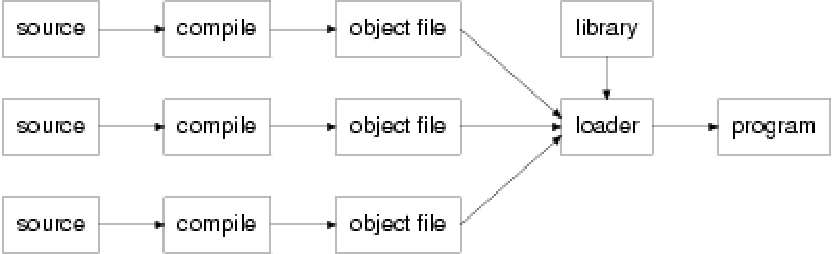
\includegraphics[type=pdf,read=.pdf,ext=.pdf,scale=0.9]
     {figure/1.1_sepComp}
     \caption*{Diagram showing multiple files going from source,
       through compilation, to object files,
       and being combined with libraries by the loader 
       to produce a program.}
     \caption{\label{fig:sepComp}Separate compilation}
   \end{figure*}


  This technique is important in C, where it is common to find all but the
   smallest of programs constructed from a number of separate source files.
   Furthermore, the extensive use that C makes of libraries means that even
   trivial programs pass through the loader, although that might not be obvious
   at the first glance or to the newcomer.


 
        \section{Functions}
        

  

  A C program is built up from a collection of items such as
   \textbf{functions} and what we could loosely call \textbf{global
   variables}. All of these things are given names at the point where they
   are defined in the program; the way that the names are used to access those
   items from a given place in the program is governed by rules. The rules are
   described in the Standard using the term \textbf{linkage}. For the moment
   we only need to concern ourselves with \textbf{external linkage} and
   \textbf{no linkage}. Items with external linkage are those that are
   accessible throughout the program (library functions are a good example);
   items with no linkage are also widely used but their accessibility is much
   more restricted. Variables used inside functions are usually `local'
   to the function; they have no linkage. Although this book avoids the use of
   complicated terms like those where it can, sometimes there isn't a plainer
   way of saying things. Linkage is a term that you are going to become
   familiar with later. The only external linkage that we will see for a while
   will be when we are using functions.


  Functions are C's equivalents of the functions and subroutines in FORTRAN,
   functions and procedures in Pascal and ALGOL. Neither BASIC in most of its
   simple mutations, nor COBOL has much like C's functions.


  The idea of a function is, of course, to allow you to encapsulate one idea
   or operation, give it a name, then to call that operation from various parts
   of the rest of your program simply by using the name. The detail of what is
   going on is not immediately visible at the point of use, nor should it
   be. In well designed, properly structured programs, it should be possible to
   change the way that a function does its job (as long as the job itself
   doesn't change) with no effect on the rest of the program.


  In a \textbf{hosted environment} there is one function whose name is
   special; it's the one called \texttt{main}. This function is the first
   one entered when your program starts running. In a \textbf{freestanding
   environment} the way that a program starts up is \textbf{implementation
   defined}; a term which means that although the Standard doesn't specify
   what must happen, the actual behaviour must be consistent and
   documented. When the program leaves the main function, the whole program
   comes to an end.
   % Here's a simple program containing two functions:
   Program \ref{prg:main} on page \pageref{prg:main}
   shows a simple program containing two functions. 


   \begin{program}[phtb]
     \verbfilenobox[\scriptsize]{example/example1-1.c}
     \caption{\label{prg:main}program with main function}
     % \begin{center}\textit{Example 1.1}\end{center}
   \end{program}


 
   \section{A description of Example 1.1}


   \subsection{What was in it}
   

   Even such a small example has introduced a lot of C. Among other
    things, it contained two functions, a \texttt{\#include}
    `statement', and some \textbf{comment}. Since comment is the
    easiest bit to handle, let's look at that first.


  

  \subsection{Layout and comment}
   

   The layout of a C program is not very important to the compiler, although
    for readability it is important to use this freedom to carry extra
    information for the human reader. C allows you to put space, tab or newline
    characters practically anywhere in the program without any special effect
    on the meaning of the program. All of those three characters are the same
    as far as the compiler is concerned and are called collectively \textbf{white
    space}, because they just move the printing position without causing
    any `visible' printing on an output device. White space can occur
    practically anywhere in a program except in the middle of
    \textbf{identifiers}, \textbf{strings}, or \textbf{character
    constants}. An identifier is simply the name of a function or some
    other object; strings and character constants will be discussed
    later--don't worry about them for the moment.


   Apart from the special cases, the only place that white space must be
    used is to separate things that would otherwise run together and become
    confused. In the example above, the fragment \texttt{void show\_message}
    needs space to separate the two words, whereas \texttt{show\_message(}
    could have space in front of the \texttt{(} or not, it would be purely
    a matter of taste.


   Comment is introduced to a C program by the pair of characters
    \texttt{/*}, which must not have a space between them. From then on,
    everything found up to and including the pair of characters \texttt{*/}
    is gobbled up and the whole lot is replaced by a single space. In Old C,
    this was not the case. The rule used to be that comment could occur
    anywhere that space could occur: the rule is now that comment is space. The
    significance of the change is minor and eventually becomes apparent in
    Chapter~\ref{chap:preproc} where we discuss the \textbf{preprocessor}. A
    consequence of the rule for the end of comment is that you can't put a
    piece of comment inside another piece, because the \textit{first}
    \texttt{*/} pair will finish all of it. This is a minor nuisance, but
    you learn to live with it.


   It is common practice to make a comment stand out by making each line of
    multi-line comment always start with a \texttt{*}, as the example
    illustrates.


  

  \subsection{Preprocessor statements}
   

   The first statement in the example is a \textbf{preprocessor
    directive}. In days gone by, the C compiler used to have two phases:
    the \textbf{preprocessor}, followed by the real compiler. The
    preprocessor was a \textbf{macro processor}, whose job was to perform
    simple textual manipulation of the program before passing the modified text
    on to be compiled.  The preprocessor rapidly became seen as an essential
    aspect of the compiler and so has now been defined as part of the language
    and cannot be bypassed.


   The preprocessor only knows about \textit{lines} of text; unlike the rest
    of the language it is sensitive to the end of a line and though it is
    possible to write multi-line preprocessor directives, they are uncommon and
    a source of some wonder when they are found. Any line whose first visible
    character is a \texttt{\#} is a preprocessor directive.


   In Example 1.1 the preprocessor directive
    \texttt{\#include} causes the line containing it to be replaced
    completely by the contents of another file. In this case the filename is
    found between the \texttt{<} and \texttt{>} brackets. This is
    a widely used technique to incorporate the text of standard \textbf{header
    files} into your program without having to go through the effort of
    typing it all yourself. The \texttt{<stdio.h>} file is an
    important one, containing the necessary information that allows you to use
    the standard library for input and output.  If you want to use the I/O
    library you \textit{must} include \texttt{<stdio.h>}. Old C was
    more relaxed on this point.


   \subsubsection{Define statements}
    

    Another of the preprocessor's talents which is widely exploited is the
     \texttt{\#define} statement. It is used like this:


    \begin{Verbatim}
#define IDENTIFIER      replacement
\end{Verbatim}

    which says that the name represented by \texttt{IDENTIFIER} will be
     replaced by the text of replacement whenever \texttt{IDENTIFIER}
     occurs in the program text. Invariably, the identifier is a name in
     upper-case; this is a stylistic convention that helps the reader to
     understand what is going on.  The replacement part can be any text at
     all--remember the preprocessor doesn't know C, it just works on
     text. The most common use of the statement is to declare names for
     constant numbers:


    \begin{Verbatim}
#define PI             3.141592
#define SECS_PER_MIN   60
#define MINS_PER_HOUR  60
#define HOURS_PER_DAY  24
\end{Verbatim}

    and to use them like this


    \begin{Verbatim}
circumf = 2*PI*radius;
if(timer >= SECS_PER_MIN){
mins = mins+1;
        timer = timer - SECS_PER_MIN;
}
\end{Verbatim}

    the output from the preprocessor will be as if you had written this:


    \begin{Verbatim}
circumf = 2*3.141592*radius;
if(timer >= 60){
        mins = mins+1;
       timer = timer - 60;
}
\end{Verbatim}

   

   \subsubsection{Summary}
    Preprocessor statements work on a line-by-line basis, the rest of C does
     not.

    \texttt{\#include} statements are used to read the contents of a
     specified file, typically to facilitate the use of library functions.

    \texttt{\#define} statements are typically used to give names for
     constants. By convention, the names are in upper case (capitalized).

   
     % interesting: macro expansion also within strings,
     % interesting would be the effect of whitespace
     % gcc -E, among other things, expands macros without compiling 
  

  \subsection{Function declaration and definition}
   

   \subsubsection{Declaration}
    

    After the \texttt{<stdio.h>} file is included comes a
     \textbf{function declaration}; it tells the compiler that
     \texttt{show\_message} is a function which takes no arguments and
     returns no values. This demonstrates one of the changes made by the
     Standard: it is an example of a \textbf{function prototype}, a subject
     which Chapter~\ref{chap:funcs} discusses in detail. It isn't always
     necessary to declare functions in advance--C will use some (old)
     default rules in such cases--but it is now strongly recommended that
     you \textit{do} declare them in advance. The distinction between a
     \textbf{declaration} and a \textbf{definition} is that the former
     simply describes the type of the function and any arguments that it might
     take, the latter is where the body of a function is provided. These terms
     become more important later.


    By declaring \texttt{show\_message} before it is used, the compiler
     is able to check that it is used correctly. The declaration describes
     three important things about the function: its name, its type, and the
     number and type of its arguments. The \texttt{void show\_message(} part
     indicates that it is a function and that it returns a value of type
     \void, which is discussed in a moment. The second use of
     \void{} is in the declaration of the function's argument list,
     \texttt{(void)}, which indicates that there are \textit{no} arguments
     to this function.


   

   \subsubsection{Definition}
    

    Right at the end of the program is the function definition itself;
     although it is only three lines long, it usefully illustrates a complete
     function.


    In C, functions perform the tasks that some other languages split into
     two parts. Most languages use a function to return a value of some sort,
     typical examples being perhaps trigonometric functions like sin, cos, or
     maybe a square root function; C is the same in this respect. Other similar
     jobs are done by what look very much like functions but which don't return
     a value: FORTRAN uses \textbf{subroutines}, Pascal and Algol call them
     \textbf{procedures}. C simply uses functions for all of those jobs, with
     the \textit{type} of the function's return value specified when the
     function is defined. In the example, the function
     \texttt{show\_message} doesn't return a value so we specify that its
     type is \void.


    The use of \void{} in that way is either crashingly obvious or
     enormously subtle, depending on your viewpoint. We could easily get
     involved here in an entertaining (though fruitless) philosophical
     side-track on whether \void{} really is a value or not, but we
     won't. Whichever side of the question you favour, it's clear that you
     can't do anything with a \void{} and that's what it means
     here--``I don't want to do anything with any value this function
     might or might not return''.


    The type of the function is \void, its name is
     \texttt{show\_message}. The parentheses \texttt{()} following
     the function name are needed to let the compiler know that at this point
     we are talking about a function and not something else. If the function
     did take any arguments, then their names would be put between the
     parentheses. This one doesn't take any, which is made explicit by putting
     \void{} between the parentheses.


    For something whose essence is emptiness, abnegation and rejection,
     \void{} turns out to be pretty useful.


    The body of the function is a \textbf{compound statement}, which is a
     sequence of other statements surrounded by curly
     brackets \texttt{\{\}}. There is only one statement in there, but
     the brackets are still needed. In general, C allows you to put a compound
     statement anywhere that the language allows the use of a single simple
     statement; the job of the brackets being to turn several statements in a
     row into what is effectively a single statement.


    It is reasonable to ask whether or not the brackets are strictly needed,
     if their only job is to bind multiple statements into one, yet all that we
     have in the example is a single statement. Oddly, the answer is
     yes--they \textit{are} strictly needed. The only place in C where you
     can't put a single statement but \textit{must} have a compound statement
     is when you are defining a function. The simplest function of all is
     therefore the empty function, which does nothing at all:


    \begin{Verbatim}
void do_nothing(void){}
\end{Verbatim}

    The statement inside show\_message is a call of the library function
     \texttt{printf}. \texttt{printf} is used to format and print
     things, this example being one of the simplest of its
     uses. \texttt{printf} takes one or more arguments, whose values are
     passed forward from the point of the call into the function itself. In
     this case the argument is a \textbf{string}. The contents of the string
     are interpreted by \texttt{printf} and used to control the way the
     values of the other arguments are printed. It bears a little resemblance
     to the FORMAT statement in FORTRAN; but not enough to predict how to use
     it.


   

   \subsubsection{Summary}
    \textbf{Declarations} are used to introduce the name of a function,
     its return type and the type (if any) of its arguments.

    A function \textbf{definition} is a declaration with the body of the
     function given too.

    A function returning no value should have its type declared as
     \void. For example,
     \texttt{void func(/* list of arguments */);}
    

    A function taking no arguments should be declared with \void{}
     as its argument list. For example, \texttt{void func(void);}

   

  

  \subsection{Strings}
   

   In C, strings are a sequence of characters surrounded by quote marks:


   \begin{Verbatim}
"like this"
\end{Verbatim}

   Because a string is a single element, a bit like an identifier, it is not
    allowed to continue across a line--although space or tab characters
    are permitted inside a string.


   \begin{Verbatim}
"This is a valid string"
"This has a newline in it
and is NOT a valid string"
\end{Verbatim}

   To get a very long string there are two things that you can do. You could
    take advantage of the fact that absolutely everywhere in a C program, the
    sequence `backslash end-of-line' disappears totally.


   \begin{Verbatim}
"This would not be valid but doesn't have \
a newline in it as far as the compiler is concerned"
\end{Verbatim}

   The other thing you could do is to to use the string joining feature,
    which says that two adjacent strings are considered to be just one.


   \begin{Verbatim}
"All this " "comes out as "
"just one string"
\end{Verbatim}

   Back to the example. The sequence `\texttt{\textbackslash n}' in the
    string is an example of an \textbf{escape} sequence which in this case
    represents `newline'. \texttt{Printf} simply prints the
    contents of the string on the program's output file, so the output will
    read `hello', followed by a new line.


   To support people working in environments that use character sets which
    are `wider' than U.S. ASCII, such as the shift-JIS representation
    used in Japan, the Standard now allows \textbf{multibyte characters} to
    be present in strings and comments. The Standard defines the
    96 characters that are the alphabet of C (see Chapter~\ref{chap:varArith}).
    If your system supports an extended character set, the only
    place that you may use these extended characters is in strings, character
    constants, comment and the names of \textbf{header files}. Support for
    extended character sets is an implementation defined feature, so you will
    have to look it up in your system's documentation.


  

  \subsection{The main function}
   

   In Example 1.1 there are actually two functions,
    \texttt{show\_message} and \texttt{main}. Although main is a bit
    longer than \texttt{show\_message} it is obviously built in the same
    shape: it has a name, the parentheses () are there, followed by the opening
    bracket \texttt{\{} of the compound statement that must follow in a
    function definition. True, there's a lot more stuff too, but right at the
    end of the example you'll find the matching closing bracket \texttt{\}}
    that goes with the first one to balance the numbers.


   This is a much more realistic function now, because there are several
    statements inside the function body, not just one. You might also have
    noticed that the function is \textit{not} declared to be
    \void. There is a good reason for this: it returns a proper
    value. Don't worry about its arguments yet; they are discussed in
    Chapter~\ref{chap:completeCprg}.


   The most important thing about \texttt{main} is that it is the first
    function to be called. In a hosted environment your C language system
    arranges, magically, for a call on the \texttt{main} function (hence
    its name) when the program is first started. When the function is over, so
    is the program. It's obviously an important function. Equally important is
    the stuff \textit{inside} \texttt{main}'s compound statement. As
    mentioned before, there can be several statements inside a compound
    statement, so let's look at them in turn.


  

  \subsection{Declarations}
   

   The first statement is this:


   \begin{Verbatim}
int count;
\end{Verbatim}

   which is not an instruction to do anything, but simply introduces a
    variable to the program. It declares something whose name is
    \texttt{count}, and whose type is `integer'; in C the
    keyword that declares integers is unaccountably shortened to
    \kint. C has an idiosyncratic approach to these keywords with
    some having their names spelled in full and some being shortened like
    \kint. At least \kint{} has a meaning that is more or
    less intuitive; just wait until we get on to \static.


   As a result of that declaration the compiler now knows that there is
    something that will be used to store integral quantities, and that its name
    is \texttt{count}. In C, all variables must be declared before they are
    used; there is none of FORTRAN's implicit declarations. In a compound
    statement, all the declarations must come first; they must precede any
    `ordinary' statements and are therefore somewhat special.


   (Note for pedants: unless you specifically ask, the declaration of a
    variable like \texttt{count} is also a \textbf{definition}. The
    distinction will later be seen to matter.)


  

  \subsection{Assignment statement}
   

   Moving down the example we find a familiar thing, an \textbf{assignment
     statement}. This is where the first value is assigned to the variable
     \texttt{count}, in this case the value assigned is a constant whose
     value is zero. Prior to the assignment, the value of \texttt{count}
     was undefined and unsafe to use. You might be a little surprised to find
     that the assignment symbol (strictly speaking an \textbf{assignment
     operator}) is a single \texttt{=} sign. This is not fashionable
     in modern languages, but hardly a major blemish.


   So far then, we have declared a variable and assigned the value of zero
    to it. What next?


  

  \subsection{The while statement}
   

   Next is one of C's loop control statements, the while statement. Look
    carefully at its form. The formal description of the \while{}
    statement is this:


   \begin{Verbatim}
while(expression)
        statement
\end{Verbatim}

   Is that what we have got? Yes it is. The bit that reads


   \begin{Verbatim}
count < 10
\end{Verbatim}

   is a \textbf{relational expression}, which is an example of a valid
    expression, and the expression is followed by a compound statement, which
    is a form of valid statement. As a result, it fits the rules for a properly
    constructed \while{} statement.


   What it does must be obvious to anyone who has written programs
    before. For as long as the relationship \texttt{count < 10} holds
    true, the body of the loop is executed and the comparison repeated. If the
    program is ever to end, then the body of the loop must do something that
    will eventually cause the comparison to be false: of course it does.


   There are just two statements in the body of the loop. The first one is a
    function call, where the function \texttt{show\_message} is invoked. A
    function call is indicated by the name of the function followed by the
    parentheses \texttt{()} which contain its argument list--if it
    takes no arguments, then you provide none. If there were any arguments,
    they would be put between the parentheses like this:


   \begin{Verbatim}
/* call a function with several arguments */
function_name(first_arg, second_arg, third_arg);
\end{Verbatim}

and so on. The call of \texttt{printf} is another example.
More is explained in Chapter~\ref{chap:funcs}.


   The last statement in the loop is another assignment statement. It adds
    one to the variable \texttt{count}, so that the requirement for program
    to stop will eventually be met.


  

  \subsection{The return statement}
   

   The last statement that is left to discuss is the \return{}
    statement. As it is written, it looks like another function call, but in
    fact the rule is that the statement is written


   \begin{Verbatim}
     return expression;
   \end{Verbatim}

   where the \textit{expression} is optional. The example uses a common
    stylistic convention and puts the \textit{expression} into parentheses,
    which has no effect whatsoever.


   The return causes a value to be returned from the current function to its
    caller. If the expression is missing, then an unknown value is passed back
    to the caller--this is almost certainly a mistake unless the function
    returns \void. \texttt{Main} wasn't declared with any type
    at all, unlike \texttt{show\_message}, so what type of value does it
    return? The answer is \kint. There are a number of places where
    the language allows you to declare things by default: the default type of
    functions is \kint, so it is common to see them used in this
    way. An equivalent declaration for \texttt{main} would have been


   \begin{Verbatim}
     int main() {
     \end{Verbatim}

   and exactly the same results would have occurred.


   You can't use the same feature to get a default type for variables
    because their types must be provided explicitly.


   What does the value returned from \texttt{main} mean, and where does
    it go? In Old C, the value was passed back to the operating system or
    whatever else was used to start the program running. In a UNIX-like
    environment, the value of \texttt{0} meant `success' in some way,
    any other value (often \texttt{-1}) meant `failure'. The Standard
    has enshrined this, stating that \texttt{0} stands for correct
    termination of the program. This \textit{does not} mean that 0 is to be
    passed back to the host environment, but whatever is the appropriate
    `success' value for that system. Because there is sometimes confusion
    around this, you may prefer to use the defined values
    \texttt{EXIT\_SUCCESS} and \texttt{EXIT\_FAILURE} instead, which are
    defined in the header file \texttt{<stdlib.h>}. Returning from
    the \texttt{main} function is the same as calling the library function
    \texttt{exit} with the return value as an argument. The difference is
    that exit may be called from \textit{anywhere} in the program, and
    terminates it at that point, after doing some tidying up activities. If you
    intend to use \texttt{exit}, you \textit{must} include the header file
    \texttt{<stdlib.h>}. From now on, we shall use \texttt{exit}
    rather than returning from \texttt{main}.


   \subsubsection{Summary}
    The \texttt{main} function returns an \kint{} value.

    Returning from \texttt{main} is the same as calling the
     \texttt{exit} function, but \texttt{exit} can be called from
     anywhere in a program.

    Returning \texttt{0} or \texttt{EXIT\_SUCCESS} is the way of
     indicating success, anything else indicates failure.

   

  

  \subsection{Progress so far}
   

   This example program, although short, has allowed us to introduce several
    important language features, amongst them:


   \begin{itemize}
    \item Program structure
    \item Comment
    \item File inclusion
    \item Function definition
    \item Compound statements
    \item Function calling
    \item Variable declaration
    \item Arithmetic
    \item Looping
   \end{itemize}

   although of course none of this has been covered rigorously.


  

 
        \section{Some more programs}
        

  

  While we're still in the informal phase, let's look at two more examples.
   You will have to work out for yourself what some of the code does, but as
   new or interesting features appear, they will be explained.


  \subsection{A program to find prime numbers}
   

   \begin{program}[phtb]
     \verbfilenobox[\scriptsize]{example/example1-2.c}
     \caption{\label{prg:prime}program to find prime numbers}
     %\begin{center}\textit{Example 1.2}\end{center}
 \end{program}
 
   What was interesting in there? A few new points, perhaps. The program
    works in a really stupid way: to see if a number is prime, it divides that
    number by all the numbers between half its value and two--if any
    divide without remainder, then the number isn't prime. The two operators
    that you haven't seen before are the remainder operator \texttt{\%},
    and the equality operator, which is a double equal sign \texttt{==}.
    That last one is without doubt the cause of more bugs in C programs than
    any other single factor.


   The problem with the equality test is that wherever it can appear it is
    also legal to put the single \texttt{=} sign. The first,
    \texttt{==}, compares two things to see if they are equal, and is
    generally what you need in fragments like these:


   \begin{Verbatim}
if(a == b)
while (c == d)
\end{Verbatim}

   The assignment operator \texttt{=} is, perhaps surprisingly, also
    legal in places like those, but of course it assigns the value of the
    right-hand expression to whatever is on the left. The problem is
    particularly bad if you are used to the languages where comparison for
    equality is done with what C uses for assignment. There's nothing that you
    can do to help, so start getting used to it now. (Modern compilers do tend
    to produce warnings when they think they have detected
    `questionable' uses of assignment operators, but that is a mixed
    blessing when your choice was deliberate.)


   There is also the introduction for the first time of the \kif{}
    statement. Like the \while{} statement, it tests an expression
    to see if the expression is true. You might have noticed that also like
    the \while{} statement, the expression that controls the
    \kif{} statement is in parentheses. That is always the case: all
    of the conditional control of flow statements require a parenthesized
    expression after the keyword that introduces them. The formal description
    of the \kif{} statement goes like this:


   \begin{Verbatim}
if(expression)
        statement

if(expression)
        statement
else
        statement
\end{Verbatim}

   showing that it comes in two forms. Of course, the effect is that if the
    expression part is evaluated to be true, then the following statement is
    executed. If the evaluation is false, then the following statement is not
    executed. When there is an \kelse{} part, the statement associated
    with it is executed only if the evaluation gives a false result.


   \kif{} statements have a famous problem. In the following piece
    of code, is the \textit{statement-2} executed or not?


   \begin{Verbatim}
if(1 > 0)
        if(1 < 0)
                statement-1
else
        statement-2
\end{Verbatim}

The answer is that it \textit{is}. Ignore the indentation (which is
misleading). The \kelse{} could belong to either the first or
second \kif, according to the description of the \kif{}
statement that has just been given, so an extra rule is needed to make it
unambiguous. The rule is simply that an \kelse{} is associated
with the nearest \kelse-less \kif{} above it. To make
the example work the way that the indentation implied, we have to invoke a
compound statement:


   \begin{Verbatim}
if(1 > 0){
        if(1 < 0)
                statement-1
}
else
        statement-2
\end{Verbatim}

   Here, at least, C adheres to the practice used by most other languages.
    In fact a lot of programmers who are used to languages where the problem
    exists have never even realized that it is there--they just thought
    that the disambiguating rule was `obvious'. Let's hope that
    everyone feels that way.


  

  \subsection{The division operators}
   

   
   The division operators are the division operator \texttt{/}, and the
    remainder operator \texttt{\%}. Division does what you would expect,
    except that when it is applied to integer operands it gives a result that
    is truncated towards zero. For example, \texttt{5/2} gives
    \texttt{2}, \texttt{5/3} gives \texttt{1}. The remainder
    operator is the way to get the truncated remainder. \texttt{5\%2} gives
    \texttt{1}, \texttt{5\%3} gives \texttt{2}. The signs of the
    remainder and quotient depend on the divisor and dividend in a way that is
    defined in the Standard and shown in Chapter~\ref{chap:varArith}.


  

  \subsection{An example performing input}
   

   It's useful to be able to perform input as well as to write programs
    that print out more or less interesting lists and tables. The simplest of
    the library routines (and the only one that we'll look at just now) is
    called \texttt{getchar}. It reads single characters from the program's
    input and returns an integer value. The value returned is a coded
    representation for that character and can be used to print the same
    character on the program output. It can also be compared against character
    constants or other characters that have been read, although the only test
    that makes sense is to see if both characters are the same. Comparing for
    greater or less than each other is not portable in general; there is no
    guarantee that \texttt{'a'} is less than \texttt{'b'}, although on
    most common systems that would be the case. The only guarantee that the
    Standard makes is that the codes for \texttt{'0'} through to
    \texttt{'9'} will always be consecutive.
    % Here is one example.
    Program \ref{prg:read} is an example. 
    % 
    \begin{program}[phtb]
      \verbfilenobox[\scriptsize]{example/example1-3.c}
      \caption{\label{prg:read}program reading in characters}
      % \begin{center}\textit{Example 1.3}\end{center}
    \end{program}
    
   There are two interesting points in there. The first is to notice that
   at the end of each line of input read, the character represented by
   %
   \begin{Verbatim}
     '\n'
   \end{Verbatim}

   (a character constant) will be seen. This just like the way that the
    same symbol results in a new line when \texttt{printf} prints it. The
    model of I/O used by C is not based on a line by line view of the world,
    but character by character instead; if you choose to think in a
    line-oriented way, then \texttt{'\textbackslash n'} allows you to mark the end of
    each `line'. Second is the way that \texttt{\%c} is used to
    output a character by \texttt{printf}, when it appears on the output
    as a character. Printing it with \texttt{\%d} prints the same variable,
    but displays the integer value used by your program to represent the
    character.


   If you try that program out, you may find that some systems do not pass
    characters one by one to a program, but make you type a whole line of
    input first. Then the whole line is made available as input, one character
    at a time. Beginners have been known to be confused: the program is
    started, they type some input, and nothing comes back. This behaviour is
    nothing to do with C; it depends on the computer and operating system in
    use.


  

  \subsection{Simple arrays}
   

   The use of \textbf{arrays} in C is often a problem for the beginner.
    The declaration of arrays isn't too difficult, especially the
    one-dimensional ones, but a constant source of confusion is the fact
    that their indices always count from 0. To declare an array of
    5 \kint{}s, the declaration would look like this:


   \begin{Verbatim}
     int something[5];
   \end{Verbatim}

   In array declarations C uses square brackets, as you can see. There is
    no support for arrays with indices whose ranges do not start at 0 and go
    up; in the example, the valid array elements are \texttt{something[0]}
    to \texttt{something[4]}. Notice very carefully that
    \texttt{something[5]} is \textit{not} a valid array element.


    This program reads some characters from its input, sorts them into the
    order suggested by their representation, then writes them back out. Work
    out what it does for yourself; the algorithm won't be given much attention
    in the explanation which follows.


    \begin{program}[phtb]
      \verbfilenobox[\scriptsize]{example/example1-4.c}
      \caption{\label{prg:readSort}program for sorting}
      %\begin{center}\textit{Example 1.4}\end{center}
    \end{program}
  
   You might note that the defined constant \texttt{ARSIZE} is used
    everywhere instead of the actual array size. Because of that, to change
    the maximum number of characters that can be sorted by this program simply
    involves a change to one line and then re-compiling. Not so obvious but
    critical to the safety of the program is the detection of the array
    becoming full. Look carefully; you'll find that the program stops when
    element \texttt{ARSIZE-1} has been filled. That is because in an
    \texttt{N} element array, only elements \texttt{0} through to
    \texttt{N-1} are available (giving \texttt{N} in total).


   Unlike some other languages it is unlikely that you will be told if you
    `run off' the end of an array in C. It results in what is known as
    \textbf{undefined behaviour} on the part of your program, this generally
    being to produce obscure errors in the future. Most skilled programmers
    avoid this happening by rigorous testing to make sure either that it can't
    happen given the particular algorithm in use, or by putting in an explicit
    test before accessing a particular member of an array. This is a common
    source of run-time errors in C; you have been warned.


  

  \subsection{Summary}
   Arrays always number from \texttt{0}; you have no choice.

   A \texttt{n}-element array has members which number from
    \texttt{0} to \texttt{n-1} only.  Element \texttt{n} does not
    exist and to access it is a big mistake.

  

 
        \section{Terminology}
        

  

  In C programs there are two distinct types of things: things used to hold
   values and things that are functions. Instead of having to refer to them
   jointly with a clumsy phrase that maintains the distinction, we think that
   it's useful to call them both loosely `objects'. We do quite a lot of
   that later, because it's often the case that they follow more or less the
   same rules. Beware though, that this isn't quite what the Standard uses the
   term to mean. In the Standard, an `object' is explicitly a region of
   allocated storage that is used to represent a value and a function is
   something different; this leads to the Standard often having to say
   `\ldots  functions and objects \ldots '. Because we don't think
   that it leads to too much confusion and does improve the readability of the
   text in most cases, we will continue to use our looser interpretation of
   object to include functions and we will explicitly use the terms `data
   objects' and `functions' when the distinction is appropriate.


  Be prepared to find this slight difference in meaning if you do read the
   Standard.


 
        \section{Summary}
        


  This chapter has introduced many of the basics of the language although
   informally. Functions, in particular, form the basic building block for C.
   Chapter~\ref{chap:funcs} provides a full description of these fundamental
   objects, but you should by now understand enough about them to follow their
   informal use in the intervening material.


  Although the idea of library functions has been introduced, it has not
   been possible to illustrate the extent of their importance to the C
   application programmer.
   The Standard Library, described in Chapter~\ref{chap:libs},
   is \textit{extremely} important, both in the way that it helps to
   improve the portability of programs intended for general use and also in
   the aid to productivity that these useful functions can provide.


  The use of variables, expressions and arithmetic are soon to be described
   in great detail. As this chapter has shown, at a simple level, C differs
   little from most other modern programming languages.


  Only the use of structured data types still remains to be introduced,
   although arrays have had a very brief airing.


 
        \section{Exercises}
        


  \textbf{Exercise 1.1.} Type in and test Example 1.1 on your
   system.


  \textbf{Exercise 1.2.} Using Example 1.2 as a pattern, write a
   program that prints prime pairs -- a pair of prime numbers that differ
   by 2, for example 11 and 13, 29 and 31. (If you can detect a pattern
   between such pairs, congratulations! You are either a genius or just
   wrong.)


  \textbf{Exercise 1.3.} Write a function that returns an integer: the decimal
   value of a string of digits that it reads using \texttt{getchar}. For
   example, if it reads 1 followed by 4 followed by 6, it will
   return the number 146.  You may make the assumption that the
   digits 0-9 are consecutive in the computer's representation (the
   Standard says so) and that the function will only have to deal with valid
   digits and newline, so error checking is not needed.


  \textbf{Exercise 1.4.} Use the function that you just wrote to read a sequence
   of numbers.  Put them into an array declared in main, by repeatedly calling
   the function. Sort them into ascending numerical order, then print the
   sorted list.


  \textbf{Exercise 1.5.} Again using the function from Exercise 1.3, write a
   program that will read numbers from its input, then print them out in
   binary, decimal and hexadecimal form. You should not use any features of
   \texttt{printf} apart from those mentioned in this chapter (especially
   the hexadecimal output format!). You are expected to work out what digits
   to print by calculating each one in turn and making sure that they are
   printed in the right order. This is not particularly difficult, but it is
   not trivial either.


 \chapter{Variables and Arithmetic}\label{chap:varArith}


        \section{Some fundamentals}
        

  

  Here is where we start to look in detail at the bits that the last
   chapter chose to sweep under the carpet while it did its
   `Instant C' introduction. The problem is, of course, the usual
   one of trying to introduce enough of the language to let you get a feel for
   what it's all about, without drowning beginners in a froth of detail that
   isn't essential at the time.


  Because this is a lengthy chapter, and because it deliberately chooses to
   cover some subtle problems that are often missed out in introductory texts,
   you should make sure that you are in the right mood and proper frame of
   mind to read it.


  The weary brain may find that the breaks for exercises are useful. We
   strongly recommend that you do actually attempt the exercises on the way
   through. They help to balance the weight of information, which otherwise
   turns into an indigestible lump.


  It's time to introduce some of the fundamentals.


 
        \section{The alphabet of C}
        

  

  This is an interesting area; alphabets are important. All the same, this
   is the one part of this chapter that you can read superficially first time
   round without missing too much. Read it to make sure that you've seen the
   contents once, and make a mental note to come back to it later on.


  \subsection{Basic Alphabet}\label{subsec:alpha}
   

   Few computer languages bother to define their alphabet rigorously.
    There's usually an assumption that the English alphabet augmented by a
    sprinkling of more or less arbitrary punctuation symbols will be available
    in every environment that is trying to support the language. The
    assumption is not always borne out by experience. Older languages suffer
    less from this sort of problem, but try sending C programs by Telex
    or restrictive e-mail links and you'll understand the difficulty.


   The Standard talks about two different character sets: the one that
    programs are written in and the one that programs execute with. This is
    basically to allow for different systems for compiling and execution,
    which might use different ways of encoding their characters. It doesn't
    actually matter a lot except when you are using character constants in the
    preprocessor, where they may not have the same value as they do at
    execution time. This behaviour is implementation-defined, so it must be
    documented. Don't worry about it yet.


    The Standard requires that an alphabet of 96 symbols 
    is available for C as follows in Table~\ref{tab:alphabetC}. 

    \begin{table}[htb]
     \centering
      \begin{tabular}{p{0.9\textwidth}}
        \toprule
        \texttt{a b c d e f g h i j k l m n o p q r s t u v w x y z}    \\
        \texttt{A B C D E F G H I J K L M N O P Q R S T U V W X Y Z}    \\
        \texttt{0 1 2 3 4 5 6 7 8 9}    \\
        \texttt{! " \# \% \& ' ( ) * + , - . /}    \\
        \texttt{: ; < = > ? [ \textbackslash ] \^ \_ \{ | \} \~}    \\
        space, horizontal and vertical tab    \\
        form feed, newline    \\
        \bottomrule
      \end{tabular}
      \caption{\label{tab:alphabetC}The Alphabet of C}
    \end{table}



   It turns out that most of the commonly used computer alphabets contain
    all the symbols that are needed for C with a few notorious exceptions. The
    C alphabetic characters shown below are missing from the International
    Standards Organization ISO 646 standard 7-bit character set, which is
    as a subset of all the widely used computer alphabets.


   \begin{Verbatim}
     # [ \ ] ^ { | } ~
   \end{Verbatim}

   To cater for systems that can't provide the full 96 characters
    needed by C, the Standard specifies a method of using the
    ISO 646 characters to represent the missing few; the technique is the
    use of \textbf{trigraphs}.


  

  \subsection{Trigraphs}
   

   Trigraphs are a sequence of three ISO 646 characters that get
    treated as if they were one character in the C alphabet; all of the
    trigraphs start with two question marks \texttt{??} which helps
    to indicate that `something funny' is going on.
    Table~\ref{tab:trigraphs} below shows the trigraphs defined in the Standard.


    \begin{table}[htb]
      \centering
      \begin{tabular}{ll}
        \toprule
        C character & Trigraph    \\
        \midrule
        \texttt{\#} & \texttt{??=}    \\
        \texttt{[}  & \texttt{??(}    \\
        \texttt{]}  & \texttt{??)}    \\
        \texttt{\{} & \texttt{??<}    \\
        \texttt{\}} & \texttt{??>}    \\
        \texttt{\textbackslash} & \texttt{??/}    \\
        \texttt{|}  & \texttt{??!}    \\
        \texttt{\~} & \texttt{??-}    \\
        \texttt{\^} & \texttt{??'}    \\
        \bottomrule
      \end{tabular}
      \caption{\label{tab:trigraphs}Trigraphs}
    \end{table}


   As an example, let's assume that your terminal doesn't have the
    \texttt{\#} symbol. To write the preprocessor line


   \begin{Verbatim}
     #define MAX     32767
   \end{Verbatim}

   isn't possible; you must use trigraph notation instead:


   \begin{Verbatim}
??=define MAX   32767
\end{Verbatim}

   Of course trigraphs will work even if you do have a
    \texttt{\#} symbol; they are there to help in difficult
    circumstances more than to be used for routine programming.


   The \texttt{?} `binds to the right', so in any sequence of
    repeated \texttt{?}s, only the two at the right could possibly be part
    of a trigraph, depending on what comes next--this disposes of any
    ambiguity.


   It would be a mistake to assume that programs written to be highly
    portable would use trigraphs `in case they had to be moved to systems
    that only support ISO 646'. If your system can handle all 96
    characters in the C alphabet, then that is what you should be using.
    Trigraphs will only be seen in restricted environments, and it is
    extremely simple to write a character-by-character translator between the
    two representations. However, all compilers that conform to the Standard
    will recognize trigraphs when they are seen.


   Trigraph substitution is the very first operation that a compiler
    performs on its input text.


  

  \subsection{Multibyte Characters}
   

   Support for multibyte characters is new in the Standard. Why?


   A very large proportion of day-to-day computing involves data that
    represents text of one form or another. Until recently, the rather
    chauvinist computing idustry has assumed that it is adequate to provide
    support for about a hundred or so printable characters (hence the
    96 character alphabet of C), based on the requirements of the
    English language--not suprising, since the bulk of the development
    of commercial computing has been in the US market. This alphabet
    (technically called the \textbf{repertoire}) fits conveniently into 7 or
    8 bits of storage, which is why the US-ASCII character set standard
    and the architecture of mini and microcomputers both give very heavy
    emphasis to the use of 8-bit bytes as the basic unit of storage.


   C also has a byte-oriented approach to data storage. The smallest
    individual item of storage that can be directly used in C is the byte,
    which is defined to be at least 8 bits in size. Older systems or
    architectures that are not designed explicitly to support this may incur a
    performance penalty when running C as a result, although there are not
    many that find this a big problem.


   Perhaps there was a time when the English alphabet was acceptable for
    data processing applications worldwide--when computers were used in
    environments where the users could be expected to adapt--but those
    days are gone. Nowadays it is absolutely essential to provide for the
    storage and processing of textual material in the native alphabet of
    whoever wants to use the system. Most of the US and Western European
    language requirements can be squeezed together into a character set that
    still fits in 8 bits per character, but Asian and other languages
    simply cannot.


   There are two general ways of extending character sets. One is to use a
    fixed number of bytes (often two) for every character. This is what the
    wide character support in C is designed to do. The other method is to use
    a shift-in shift-out coding scheme; this is popular over 8-bit
    communication links. Imagine a stream of characters that looks like:


   \begin{Verbatim}
a b c <SI> a b g <SO> x y
\end{Verbatim}

   where \texttt{<SI>} and \texttt{<SO>} mean
    `switch to Greek' and `switch back to English'
    respectively. A display device that agreed to use that method might well
    then display a, b, c, alpha, beta, gamma, x and y. This is roughly the
    scheme used by the shift-JIS Japanese standard, except that once the
    shift-in has been seen, \textit{pairs} of characters together are used as
    the code for a single Japanese character. Alternative schemes exist which
    use more than one shift-in character, but they are less common.


   The Standard now allows explicitly for the use of extended character
    sets. Only the 96 characters defined earlier are used for the C part
    of a program, but in comments, strings, character constants and header
    names (these are really data, not part of the program as such) extended
    characters are permitted if your environment supports them. The Standard
    lays down a number of pretty obvious rules about how you are allowed to
    use them which we will not repeat here. The most significant one is that a
    byte whose value is zero is interpreted as a \textbf{null character}
    irrespective of any shift state. That is important, because C uses a null
    character to indicate the end of strings and many library functions rely
    on it. An additional requirement is that multibyte sequences must start
    and end in the initial shift state.


   The \kchar{} type is specified by the Standard as suitable to
    hold the value of all of the characters in the `execution character
    set', which will be defined in your system's documentation. This means
    that (in the example above) it could hold the value of
    `\texttt{a}' or `\texttt{b}' or even the "switch to
    Greek" character itself. Because of the shift-in shift-out mechanism,
    there would be no difference between the value stored in a char that was
    intended to represent `\texttt{a}' or the Greek `alpha'
    character. To do that would mean using a different representation -
    probably needing more than 8 bits, which on many systems would be too big
    for a \kchar. That is why the Standard introduces the
    \texttt{wchar\_t}type. To use this, you must include the
    <stddef.h> header, because \texttt{wchar\_t} is simply defined as
    an alternative name for one of C's other types. We discuss it further in
    Section~\ref{sec:exprArith}.


  

  \subsection{Summary}

   \begin{itemize}
    \item C requires at least 96 characters in the source program character
     set.
    \item Not all character sets in common use can stretch to 96 characters,
     trigraphs allow the basic ISO 646 character set to be used (at a
     pinch).
    \item Multibyte character support has been added by the Standard, with
     support for
     \begin{itemize}
      \item Shift-encoded multibyte characters, which can be squeezed into
       `ordinary' character arrays, so still have \kchar
       type.
      \item Wide characters, each of which may use more storage than a regular
       character. These usually have a different type from
       \kchar.
     \end{itemize}
    
   \end{itemize}

  

 
        \section{The Textual Structure of Programs}
        

  

  \subsection{Program Layout}
   

   The examples so far have used the sort of indentation and line layout
    that is common in languages belonging to the same family as C. They
    are `free format' languages and you are expected to use that freedom
    to lay the program out in a way that enhances its readability and
    highlights its logical structure. Space (including horizontal tab)
    characters can be used for indentation anywhere except in identifiers or
    keywords without any effect on the meaning of the program. New lines work
    in the same way as space and tab \textit{except} on preprocessor command
    lines, which have a line-by-line structure.


   If a line is getting too long for comfort there are two things you can
    do. Generally it will be possible to replace one of the spaces by a
    newline and use simply two lines instead, as this example shows.


   \begin{Verbatim}
/* a long line */
a = fred + bill * ((this / that) * sqrt(3.14159));
/* the same line */
a = fred + bill *
        ((this / that) *
        sqrt(3.14159));
\end{Verbatim}

   If you're unlucky it may not be possible to break the lines like that.
    The preprocessor suffers most from the problem, because of its reliance
    on single-line `statements'. To help, it's useful to know that the
    sequence `backslash newline' becomes invisible to the C translation
    system. As a result, the sequence is valid even in unusual places such as
    the middle of identifiers, keywords, strings and so on. Only trigraphs
    are processed before this step.


   \begin{Verbatim}
/*
 * Example of the use of line joining
 */
#define IMPORTANT_BUT_LONG_PREPROCESSOR_TEXT \
printf("this is effectively all ");\
printf("on a single line ");\
printf("because of line-joining\n");
\end{Verbatim}

   The only time that you might want to use this way of breaking lines
    (outside of preprocessor control lines) is to prevent long strings from
    disappearing off the right-hand side of a program listing. New lines are
    \textit{not} permitted inside strings and character constants, so you
    might think that the following is a good idea.


   \begin{Verbatim}
/* not a good way of folding a string */
printf("This is a very very very\
long string\n");
\end{Verbatim}

   That will certainly work, but for strings it is preferable to make use
    of the string-joining feature introduced by the Standard:


   \begin{Verbatim}
/* This string joining will not work in Old C */
printf("This is a very very very"
       "long string\n");
\end{Verbatim}

   The second example allows you to indent the continuation portion of the
    string without changing its meaning; adding indentation in the first
    example would have put the indentation into the string.


   Incidentally, both examples contain what is probably a mistake. There
    is no space in front of the `long' in the continuation string,
    which will contain the sequence `verylong' as a result. Did you
    notice?


  

  \subsection{Comment}
   

   Comment, as has been said already, is introduced by the character
    pair \texttt{/*} and terminated by \texttt{*/}. It is
    translated into a single space wherever it occurs and so it follows
    exactly the same rules that spaces do. It's important to realize that it
    doesn't simply disappear, which it used to do in Old C, and that it
    is not possible to put comment into strings or character constants.
    Comment in such a place becomes part of the string or constant:


   \begin{Verbatim}
/*"This is comment"*/
"/*The quotes mean that this is a string*/"
\end{Verbatim}

   Old C was a bit hazy about what the deletion of comment implied.
    You could argue that


   \begin{Verbatim}
int/**/egral();
\end{Verbatim}

   should have the comment deleted and so be taken by the compiler to be a
    call of a function named \texttt{integral}. The Standard C rule is
    that comment is to be read as if were a space, so the example must be
    equivalent to


   \begin{Verbatim}
int egral();
\end{Verbatim}

   which declares a function \texttt{egral} that returns type
    \kint.


  

  \subsection{Translation phases}
   

   The various character translation, line joining, comment recognition
    and other early phases of translation must be specified to occur in a
    certain order. The Standard says that the translation is to proceed as if
    the phases occurred in this order (there are more phases, but these are
    the important ones):


   \begin{enumerate}
    \item Trigraph translation.
    \item Line joining.
    \item Translate comment to space (but not in strings or character
     constants). At this stage, multiple white spaces may optionally be
     condensed into one.
    \item Translate the program.
   \end{enumerate}

   Each stage is completed before the next is started.


  

 
        \section{Keywords and identifiers}
        

  

  After covering the underlying alphabet, we can look at more interesting
   elements of C. The most obvious of the language elements are
   \textbf{keywords} and \textbf{identifiers}; their forms are identical
   (although their meanings are different).


  \subsection{Keywords}
   

   C keeps a small set of \textbf{keywords} for its own use. These
    keywords cannot be used as identifiers in the program -- a common
    restriction with modern languages. Where users of Old C may be surprised
    is in the introduction of some new keywords; if those names were used as
    identifiers in previous programs, then the programs will have to be
    changed. It will be easy to spot, because it will provoke your compiler
    into telling you about invalid names for things. Here is the list of
    keywords used in Standard C; you will notice that none of them use
    upper-case letters.

    \begin{table}[htb]
      \centering
      \begin{tabular}{llll}
        \toprule
        \auto     & \double & \kint     & \struct   \\
        \kbreak   & \kelse  & \klong    & \switch   \\
        \case     & \enum   & \register & \typedef  \\
        \kchar    & \extern & \return   & \union    \\
        \const    & \float  & \short    & \unsigned \\
        \continue & \for    & \signed   & \void     \\
        \default  & \goto   & \sizeof   & \volatile \\
        \kdo      & \kif    & \static   & \while    \\
        \bottomrule
      \end{tabular}
      \caption{\label{tab:keywords}Keywords}
    \end{table}


   The new keywords that are likely to surprise old programmers are:
   \const, \signed, \void{} and volatile{}
   (although \void{} has been around for a while).
   Eagle eyed readers may have noticed that some implementations of
   C used to use the keywords \texttt{entry}, \texttt{asm}, and
   \texttt{fortran}. These are not part of the Standard, and few will
   mourn them.


  

  \subsection{Identifiers}
   

   \textbf{Identifier} is the fancy term used to mean `name'.
    In C, identifiers are used to refer to a number of things: we've
    already seen them used to name variables and functions. They are also
    used to give names to some things we haven't seen yet, amongst which are
    \textbf{labels} and the `tags' of \textbf{structures},
    \textbf{unions}, and \textbf{enums}.


   The rules for the construction of identifiers are simple: you may use
    the 52 upper and lower case alphabetic characters, the 10 digits and
    finally the underscore `\texttt{\_}', which is considered to be
    an alphabetic character for this purpose. The only restriction is the
    usual one; identifiers \textit{must} start with an alphabetic
    character.


   Although there is no restriction on the length of identifiers in the
    Standard, this is a point that needs a bit of explanation. In Old C,
    as in Standard C, there has \textit{never} been any restriction on
    the length of identifiers. The problem is that there was never any
    guarantee that more than a certain number of characters would be checked
    when names were compared for equality--in Old C this was eight
    characters, in Standard C this has changed to 31.


   So, practically speaking, the new limit is
    31 characters--although identifiers \textit{may} be longer, they
    must differ in the first 31 characters if you want to be sure that
    your programs are portable. The Standard allows for implementations to
    support longer names if they wish to, so if you do use longer names, make
    sure that you don't rely on the checking stopping at 31.


   One of the most controversial parts of the Standard is the length of
    \textbf{external identifiers}. External identifiers are the ones that
    have to be visible outside the current source code file. Typical examples
    of these would be library routines or functions which have to be called
    from several different source files.


   The Standard chose to stay with the old restrictions on these external
    names: they are not guaranteed to be different unless they differ from
    each other in the first six characters. Worse than that, upper and lower
    case letters may be treated the same!


   The reason for this is a pragmatic one: the way that most
    C compilation systems work is to use operating system specific tools
    to bind library functions into a C program. These tools are outside
    the control of the C compiler writer, so the Standard has to impose
    realistic limits that are likely to be possible to meet. There is nothing
    to prevent any specific implementation from giving better limits than
    these, but for maximum portability the six monocase characters must be
    all that you expect. The Standard warns that it views both the use of
    only one case and any restriction on the length of external names to less
    than 31 characters as obsolescent features. A later standard may
    insist that the restrictions are lifted; let's hope that it is soon.


  

 
        \section{Declaration of variables}
        

  

  You may remember that in Chapter~\ref{chap:intro} we said that you have to
   declare the names of things before you can use them (the only exceptions to
   this rule are the names of functions returning \kint, because
   they are declared by default, and the names of \textbf{labels}). You can
   do it either by using a \textbf{declaration}, which introduces just the
   name and type of something but allocates no storage, or go further by using
   a \textbf{definition}, which also allocates the space used by the thing
   being declared.


  The distinction between declaration and definition is an important one,
   and it is a shame that the two words sound alike enough to cause confusion.
   From now on they will have to be used for their formal meaning, so if you
   are in doubt about the differences between them, refer back to this
   point.


  The rules about what makes a declaration into a definition are rather
   complicated, so they will be deferred for a while. In the meantime, here
   are some examples and rule-of-thumb guidelines which will work for the
   examples that we have seen so far, and will do for a while to come.


  \begin{Verbatim}
/*
 * A function is only defined if its body is given
 * so this is a declaration but not a definition
 */
int func_dec(void);

/*
 * Because this function has a body, it is also a definition.
 * Any variables declared inside will be definitions,
 * unless the keyword 'extern' is used.
 * Don't use 'extern' until you understand it!
 */
int def_func(void){
     float f_var;            /* a definition */
     int counter;            /* another definition */
     int rand_num(void);     /* declare (but not define) another function */

     return(0);
}
\end{Verbatim}

  

   \textbf{Exercise 2.1.} Why are trigraphs used?


   \textbf{Exercise 2.2.} When would you expect to find them in use, and when
    not?


   \textbf{Exercise 2.3.} When is a newline not equivalent to a space or
    tab?


   \textbf{Exercise 2.4.} When would you see the sequence of `backslash
    newline' in use?


   \textbf{Exercise 2.5.} What happens when two strings are put side by
    side?


   \textbf{Exercise 2.6.} Why can't you put one piece of comment inside another
    one? (This prevents the technique of `commenting out' unused bits of
    program, unless you are careful.)


   \textbf{Exercise 2.7.} What are the longest names that may safely be used for
    variables?


   \textbf{Exercise 2.8.} What is a declaration?


   \textbf{Exercise 2.9.} What is a definition?


  

  Now we go on to look at the \textbf{type} of variables and
   expressions.


 
        \section{Real types}
        

  

  It's easier to deal with the real types first because there's less to say
   about them and they don't get as complicated as the integer types. The
   Standard breaks new ground by laying down some basic guarantees on the
   precision and range of the real numbers; these are found in the header file
   \textbf{float.h} which is discussed in detail in Chapter~\ref{chap:libs}.
   For some users this is extremely important information, but it is of a
   highly technical nature and is likely only to be fully understood by
   numerical analysts.


  The varieties of real numbers are these:


  \begin{Verbatim}
    float
    double
    long double
  \end{Verbatim}

  Each of the types gives access to a particular way of representing real
  numbers in the target computer. If it only has one way of doing things,
  they might all turn out to be the same; if it has more than three, then C
  has no way of specifying the extra ones. The type \float{} is
  intended to be the small, fast representation corresponding to what FORTRAN
  would call \texttt{REAL}. You would use \double{} for extra
  precision, and \texttt{long double} for even more.


  The main points of interest are that in the increasing `lengths' of
   \float, \double{} and \texttt{long double}, each
   type must give at least the same range and precision as the previous type.
   For example, taking the value in a \double{} and putting it into
   a \texttt{long double} must result in the same value.


  There is no requirement for the three types of `real' variables to
   differ in their properties, so if a machine only has one type of real
   arithmetic, all of C's three types could be implemented in the same way.
   None the less, the three types would be considered to be different from the
   point of view of type checking; it would be `as if' they really were
   different. That helps when you move the program to a system where the three
   types really are different--there won't suddenly be a set of
   warnings coming out of your compiler about type mismatches that you didn't
   get on the first system.


  In contrast to more `strongly typed' languages, C permits
   expressions to mix all of the scalar types: the various flavours of
   integers, the real numbers and also the pointer types. When an expression
   contains a mixture of arithmetic (integer and real) types there are
   implicit conversions invoked which can be used to work out what the overall
   type of the result will be. These rules are quite important and are known
   as the \textbf{usual arithmetic conversions}; it will be worth committing
   them to memory later.
   The full set of rules is described in Section~\ref{sec:exprArith};
   for the moment, we will investigate only the ones that involve
   mixing \float, \double{} and \texttt{long double}
   to see if they make sense.


  The only time that the conversions are needed is when two different types
   are mixed in an expression, as in the example below:


   \VerbatimInput{example/example2-1.c}
   \begin{center}\textit{Example 2.1}\end{center}


  There are a lot of forced conversions in that example. Getting the
   easiest of them out of the way first, let's look at the assignments of the
   constant value \texttt{1} to each of the variables. As the section
   on constants will point out, that \texttt{1} has type \kint,
   i.e. it is an integer, not a real constant. The assignment converts the
   integer value to the appropriate real type, which is easy to cope with.


  The interesting conversions come next. The first of them is on the
   line


  \begin{Verbatim}
    d_var = d_var + f_var;
\end{Verbatim}

  What is the type of the expression involving the \texttt{+} operator?
   The answer is easy when you know the rules. Whenever two different real
   types are involved in an expression, the lower precision type is first
   implicitly converted to the higher precision type and then the arithmetic
   is performed at that precision. The example involves both a
   \double{} and a \float, so the value of
   \texttt{f\_var} is converted to type \double{} and is then
   added to the value of the double \texttt{d\_var}. The result of the
   expression is naturally of type \double{} too, so it is clearly
   of the correct type to assign to \texttt{d\_var}.


  The second of the additions is a little bit more complicated, but still
   perfectly O.K. Again, the value of \texttt{f\_var} is converted and the
   arithmetic performed with the precision of \double, forming the
   sum of the two variables. Now there's a problem. The result (the sum) is
   \double, but the assignment is to a \texttt{long double}.
   Once again the obvious procedure is to convert the lower precision value to
   the higher one, which is done, and then make the assignment.


  So we've taken the easy ones. The difficult thing to see is what to do
   when forced to assign a higher precision result to a lower precision
   destination. In those cases it may be necessary to lose precision, in a way
   specified by the implementation. Basically, the implementation must specify
   whether and in what way it rounds or truncates. Even worse, the destination
   may be unable to hold the value at all. The Standard says that in these
   cases loss of precision may occur; if the destination is unable to hold the
   necessary value--say by attempting to add the largest representable
   number to itself--then the behaviour is undefined, your program is
   faulty and you can make no predictions whatsoever about any subsequent
   behaviour.


  It is no mistake to re-emphasize that last statement. What the Standard
   means by \textbf{undefined behaviour} is exactly what it says. Once a
   program's behaviour has entered the undefined region, absolutely anything
   can happen. The program might be stopped by the operating system with an
   appropriate message, or just as likely nothing observable would happen and
   the program be allowed to continue with an erroneous value stored in the
   variable in question. It is your responsibility to prevent your program
   from exhibiting undefined behaviour. Beware!


  \subsection{Summary of real arithmatic}

   \begin{itemize}
   \item
     Arithmetic with any two real types is done
     at the highest precision of the members involved.
   \item
     Assignment involves loss of precision if the receiving type has a lower
     precision than the value being assigned to it.
   \item
     Further conversions are often implied when expressions mix other types,
     but they have not been described yet.
   \end{itemize}

  

  \subsection{Printing real numbers}
   

   The usual output function, \texttt{printf}, can be used to format
    real numbers and print them. There are a number of ways to format these
    numbers, but we'll stick to just one for now.
    Table~\ref{tab:formatReal} below
    shows the appropriate format description for each of the real types.


    \begin{table}[htb]
      \centering
      \begin{tabular}{ll}
        \toprule
        Type                 & Format        \\
        \midrule
        \float{}             & \texttt{\%f}  \\
        \double{}            & \texttt{\%f}  \\
        \texttt{long double} & \texttt{\%lf} \\
        \bottomrule
      \end{tabular}
      \caption{\label{tab:formatReal}Format codes for real numbers}
    \end{table}


   Here's an example to try:


   \VerbatimInput{example/example2-2.c}
   \begin{center}\textit{Example 2.2}\end{center}


   Try that example on your own computer to see what results you get.


  

  

   \textbf{Exercise 2.10.} Which type of variable can hold the largest range of
    values?


   \textbf{Exercise 2.11.} Which type of variable can store values to the
    greatest precision?


   \textbf{Exercise 2.12.} Are there any problems possible when assigning a
    \float{} or \double{} to a \double{} or
    \texttt{long double}?


   \textbf{Exercise 2.13.} What could go wrong when assigning, say, a \texttt{long
    double} to a \double?


   \textbf{Exercise 2.14.} What predictions can you make about a program showing
    `undefined behaviour'?


  

 
        \section{Integral types}
        

  

  The real types were the easy ones. The rules for the integral types are
   more complicated, but still tolerable, and these rules really should be
   learnt. Fortunately, the only types used in C for routine data storage are
   the real and integer types, or \textbf{structures} and \textbf{arrays}
   built up from them. C doesn't have special types for character
   manipulation or the handling of logical (boolean) quantities, but uses the
   integral types instead. Once you know the rules for the reals and the
   integers you know them all.


  We will start by looking at the various types and then the conversion
   rules.


  \subsection{Plain integers}
   

   There are two types (often called `flavours') of integer
    variables. Other types can be built from these, as we'll see, but the
    plain undecorated \texttt{ints} are the base. The most obvious of the
    pair is the `signed' \kint, the less obvious is its close
    relative, the \texttt{unsigned int}. These variables are supposed to
    be stored in whatever is the most convenient unit for the machine running
    your program. The \kint{} is the natural choice for undemanding
    requirements when you just need a simple integral variable, say as a
    counter in a short loop. There isn't any guarantee about the number of
    bits that an int can hold, except that it will \textit{always} be 16 or
    more. The standard header file \texttt{<limits.h>} details the
    actual number of bits available in a given implementation.


   Curiously, Old C had no guarantee whatsoever about the length of an
    \kint, but consensus and common practice has always assumed at
    least 16 bits.


   Actually, \texttt{<limits.h>} doesn't quite specify a number
    of bits, but gives maximum and minimum values for an \kint{}
    instead. The values it gives are 32767 and -32767 which implies
    16 bits or more, whether ones or twos complement arithmetic is used.
    Of course there is nothing to stop a given implementation from providing a
    greater range in either direction.


   The range specified in the Standard for an \texttt{unsigned int} is
    0 to at least 65535, meaning that it cannot be negative. More about
    these shortly.


   If you aren't used to thinking about the number of bits in a given
    variable, and are beginning to get worried about the portability
    implications of this apparently machine-dependent concern for the number
    of bits, then you're doing the right thing. C takes portability
    seriously and actually bothers to tell you what values and ranges are
    guaranteed to be safe. The bitwise operators encourage you to think about
    the number of bits in a variable too, because they give direct access to
    the bits, which you manipulate one by one or in groups. Almost
    paradoxically, the overall result is that C programmers have a
    healthy awareness of portability issues which leads to more portable
    programs. This is \textit{not} to say that you can't write C programs
    that are horribly non-portable!


  

  \subsection{Character variables}
   

   A bit less obvious than int is the other of the plain integral types,
    the \kchar. It's basically just another sort of
    \kint, but has a different application. Because so many
    C programs do a lot of character handling, it's a good idea to
    provide a special type to help, especially if the range provided by an
    \kint{} uses up much more storage than is needed by characters.
    The limits file tells us that three things are guaranteed about
    \kchar{} variables: they have at least 8 bits, they can store a
    value of at least +127, and the minimum value of a \kchar{}
    is zero or lower. This means that the only guaranteed range
    is 0-127. Whether or not \kchar{} variables behave as
    \signed{} or \unsigned{} types is implementation
    defined.


   In short, a character variable will probably take less storage than an
    \kint{} and will most likely be used for character manipulation.
    It's still an integer type though, and can be used for arithmetic, as this
    example shows.


    \VerbatimInput{example/example2-3.c}
    \begin{center}\textit{Example 2.3}\end{center}


   Running that program is left as an exercise for the easily amused. If
    you are bothered about where \texttt{CHAR\_MIN} and
    \texttt{CHAR\_MAX} come from, find \texttt{limits.h} and read
    it.


   Here's a more enlightening example. It uses character constants, which
    are formed by placing a character in single quotes:


   \begin{Verbatim}
     'x'
   \end{Verbatim}

   Because of the rules of arithmetic, the type of this sort of constant
    turns out to be \kint, but that doesn't matter since their
    value is always small enough to assign them to \kchar{} variables
    without any loss of precision. (Unfortunately, there is a related version
    where that guarantee does not hold. Ignore it for the moment.) When a
    character variable is printed using the \texttt{\%c} format with
    \texttt{printf}, the appropriate character is output. You can use
    \texttt{\%d}, if you like, to see what integer value is used to
    represent the character. Why \texttt{\%d}? Because a \texttt{char}
    is just another integral type.


   It's also useful to be able to read characters into a program. The
    library function \texttt{getchar} is used for the job. It reads
    characters from the program's \textbf{standard input} and returns an
    \kint{} value suitable for storing into a \kchar. The
    int value is for one reason only: not only does getchar return all
    possible character values, but it also returns an \textit{extra} value to
    indicate that end-of-input has been seen. The range of a \texttt{char}
    might not be enough to hold this extra value, so the int has to be
    used.


   The following program reads its input and counts the number of commas
    and full stops that it sees. On end-of-input, it prints the totals.


    \VerbatimInput{example/example2-4.c}
    \begin{center}\textit{Example 2.4}\end{center}


   The two features of note in that example were the multiple assignment to
    the two counters and the use of the defined constant \texttt{EOF}.
    \texttt{EOF} is the value returned by \texttt{getchar} on end of
    input (it stands for End Of File), and is defined in
    \texttt{<stdio.h>}. The multiple assignment is a fairly common
    feature of C programs.


   Another example, perhaps. This will either print out the whole lower
    case alphabet, if your implementation has its characters stored
    consecutively, or something even more interesting if they aren't.
    C doesn't make many guarantees about the ordering of characters in
    internal form, so this program produces \textit{non-portable} results!


    \VerbatimInput{example/example2-5.c}
    \begin{center}\textit{Example 2.5}\end{center}


   Yet again this example emphasizes that a \kchar{} is only
    another form of integer variable and can be used just like any other form
    of variable. It is \textit{not} a `special' type with its own
    rules.


   The space saving that a \kchar{} offers when compared to an
    \kint{} only becomes worthwhile if a lot of them are being used.
    Most character-processing operations involve the use of not just one or
    two character variables, but large arrays of them. That's when the saving
    can become noticeable: imagine an array of 1024 \kint{}s. On
    a lot of common machines that would eat up 4096 8-bit bytes of
    storage, assuming the common length of 4 bytes per \kint.
    If the computer architecture allows it to be done in a reasonably
    efficient way, the C implementor will probably have arranged for
    \kchar{} variables to be packed one per byte, so the array would
    only use 1024 bytes and the space saving would be
    3072 bytes.


   Sometimes it doesn't matter whether or not a program tries to save
    space; sometimes it does. At least C gives you the option of choosing an
    appropriate type.


  

  \subsection{More complicated types}
   

   The last two types were simple, in both their declaration and subsequent
    use. For serious systems programming they just aren't adequate in the
    precision of control over storage that they provide and the behaviour that
    they follow. To correct this problem, C provides extra forms of
    integral types, split into the categories of \signed{} and
    \unsigned. (Although both these terms are reserved words, they
    will also be used as adjectives.) The difference between the two types is
    obvious. Signed types are those that are capable of being negative, the
    unsigned types cannot be negative at any time. Unsigned types are usually
    used for one of two reasons: to get an extra bit of precision, or when the
    concept of being negative is simply not present in the data that is being
    represented. The latter is by far the better reason for choosing them.


   Unsigned types also have the special property of never overflowing in
    arithmetic. Adding 1 to a signed variable that already contains the
    maximum possible positive number for its type will result in overflow, and
    the program's behaviour becomes undefined. That can never happen with
    unsigned types, because they are defined to work `modulo one greater
    than the maximum number that they can hold'. What this means is best
    illustrated by example:


    \VerbatimInput{example/example2-6.c}
    \begin{center}\textit{Example 2.6}\end{center}


   Assuming that the variable \texttt{x} is stored in
    16 bits, then its range of values will be 0-65535 and that
    sequence will be printed endlessly. The program can't terminate: the
    test


   \begin{Verbatim}
     x >= 0
   \end{Verbatim}

   must always be true for an unsigned variable.


   For both the signed and unsigned integral types there are three
    subtypes: \short, ordinary and \klong. Taking those
    into account, here is a list of all of the possible integral types
    in C, except for the character types:


   \begin{Verbatim}
     unsigned short int
     unsigned int
     unsigned long int
     signed short int
     signed int
     signed long int
   \end{Verbatim}

   In the last three, the \signed{} keyword is unnecessary
    because the \kint{} types are signed types anyway: you
    \textit{have} to say \unsigned{} to get anything different. It's
    also permissible, but not recommended, to drop the int keyword from any of
    those declarations provided that there is at least one other keyword
    present--the \kint{} will be `understood' to be
    present. For example \klong{} is equivalent to \texttt{signed long
    int}. The long and short kinds give you more control over the amount
    of space used to store variables. Each has its own minimum range specified
    in \texttt{<limits.h>} which in practice means at least
    16 bits in a \short{} and an \kint, and at least
    32 bits in a \klong, whether signed or unsigned. As
    always, an implementation can choose to give you more bits than the
    minimum if it wants to. The only restriction is that the limits must be
    equalled or bettered, and that you don't get more bits in a shorter type
    than a longer one (not an unreasonable rule).


   The only character types are the \texttt{signed char} and the
    \texttt{unsigned char}. The difference between \kchar{} and
    \kint{} variables is that, unless otherwise stated, all
    \texttt{ints} are signed. The same is not true for \texttt{chars},
    which are signed or unsigned depending on the implementor's choice; the
    choice is presumably taken on efficiency grounds. You can of course
    explicitly force signed or unsignedness with the right keyword. The only
    time that it is likely to matter is if you are using character variables
    as extra short \texttt{shorts} to save more space.


  

  \subsection{Summary of integral types}

   \begin{itemize}
    \item The integral types are the \short, \klong,
     \signed, \unsigned{} and plain
     \texttt{ints}.
    \item The commonest is the ordinary \kint, which is signed unless
     declared not to be.
    \item The \kchar{} variables \textit{can} be made signed or
     unsigned, as you prefer, but in the absence of indications to the
     contrary, they will be allocated the most efficient type.
   \end{itemize}

  

  \subsection{Printing the integral types}
   

   Once again you can use \texttt{printf} to print these various types.
    Character variables work exactly the same way that the other integral
    variables do, so you can use the standard format letters to print their
    contents--although the actual numbers stored in them are not likely
    to be very interesting. To see their contents interpreted as characters,
    use \texttt{\%c} as was done earlier. All of the integral types can be
    printed as if they were signed decimal numbers by using the
    \texttt{\%d} format, or \texttt{\%ld} for long types. Other useful
    formats are shown in Table~\ref{tab:formatAdd}; notice that in every case a
    letter `l' is put in front of the normal format letter if a
    \klong{} is to be printed. That's not just there to get the right
    result printed: the behaviour of \texttt{printf} is undefined if the
    wrong format is given.

    \begin{table}[htb]
      \centering
      \begin{tabular}{ll}
        \toprule
        Format        & Use with    \\
        \midrule
        \texttt{\%c}  & \kchar{} (in character form)    \\
        \texttt{\%d}  & decimal \texttt{signed int}, \short, \kchar   \\
        \texttt{\%u}  & decimal \texttt{unsigned int}, \texttt{unsigned short},
                        \texttt{unsigned char}
        \\
        \texttt{\%x}  & hexadecimal \kint, \short,  \kchar    \\
        \texttt{\%o}  & octal \kint, \short, \kchar    \\
        \texttt{\%ld} & decimal \texttt{signed long}    \\
        \texttt{\%lu \%lx \%lo} & as above, but for \klong{}s    \\
        \bottomrule
      \end{tabular}
      \caption{\label{tab:formatAdd}More format codes}
    \end{table}
    

   A full description of the format codes that you can use with printf is
    given in Chapter~\ref{chap:libs}.


  

 
        \section{Expressions and arithmetic}\label{sec:exprArith}
        

  

  Expressions in C can get rather complicated because of the number of
   different types and operators that can be mixed together. This section
   explains what happens, but can get deep at times. You may need to re-read
   it once or twice to make sure that you have understood all of the
   points.


  First, a bit of terminology. Expressions in C are built from
   combinations of \textbf{operators} and \textbf{operands}, so for
   example in this expression


  \begin{Verbatim}
x = a+b*(-c)
\end{Verbatim}

  we have the operators \texttt{=}, \texttt{+} \texttt{*}
   and \texttt{-}. The operands are the
   variables \texttt{x}, \texttt{a}, \texttt{b}
   and \texttt{c}. You will also have noticed that parentheses can be
   used for grouping sub-expressions such as the \texttt{-c}. Most of
   C's unusually rich set of operators are either \textbf{binary operators},
   which take two operands, or \textbf{unary operators}, which take only
   one. In the example, the \texttt{-} was being used as a unary
   operator, and is performing a different task from the binary subtraction
   operator which uses the same \texttt{-} symbol. It may seem like
   hair-splitting to argue that they are different operators when the job that
   they do seems conceptually the same, or at least similar. It's worth doing
   though, because, as you will find later, some of the operators have both a
   binary and a unary form where the two meanings bear no relation to each
   other; a good example would be the binary multiplication
   operator \texttt{*}, which in its unary form means indirection via
   a pointer variable!


  A peculiarity of C is that operators may appear consecutively in
   expressions without the need for parentheses to separate them. The previous
   example could have been written as


  \begin{Verbatim}
x = a+b*-c;
\end{Verbatim}

  and still have been a valid expression. Because of the number of
   operators that C has, and because of the strange way that assignment works,
   the \textbf{precedence} of the operators (and their
   \textbf{associativity}) is of much greater importance to the
   C programmer than in most other languages. It will be discussed fully
   after the introduction of the important arithmetic operators.


  Before that, we must investigate the type conversions that may occur.


  \subsection{Conversions}
   

   C allows types to be mixed in expressions, and permits operations that
    result in type conversions happening implicitly. This section describes
    the way that the conversions must occur. Old C programmers should read
    this carefully, because the rules have changed -- in particular, the
    promotion of \float{} to \double, the promotions of
    short integral types and the introduction of \textbf{value preserving}
    rules are genuinely different in Standard C.


   Although it isn't directly relevant at the moment, we must note that the
    integral and the floating types are jointly known as \textbf{arithmetic
    types} and that C also supports other types (notably pointer types).
    The rules that we discuss here are appropriate only in expressions that
    have arithmetic types throughout - additional rules come into play when
    expressions mix pointer types with arithmetic types and these are
    discussed much later.


   There are various types of conversion in arithmetic expressions:


   \begin{itemize}
    \item The \textbf{integral promotions}
    \item Conversions between integral types
    \item Conversions between floating types
    \item Conversions between floating and integral types
   \end{itemize}

   Conversions between floating (real) types
   were discussed in Section~\ref{sec:exprArith};
   what we do next is to specify how the other conversions are
    to be performed, then look at \textit{when} they are required. You will
    need to learn them by heart if you ever intend to program seriously
    in C.


   The Standard has, among some controversy, introduced what are known as
    \textbf{value preserving} rules, where a knowledge of the target
    computer is required to work out what the type of an expression will be.
    Previously, whenever an unsigned type occurred in an expression, you knew
    that the result had to be \unsigned{} too. Now, the result will
    only be \unsigned{} if the conversions demand it; in many cases
    the result will be an ordinary \signed{} type.


   The reason for the change was to reduce some of the surprises possible
    when you mix signed and unsigned quantities together; it isn't always
    obvious when this has happened and the intention is to produce the
    `more commonly required' result.


   \subsubsection{Integral promotions}
    

    No arithmetic is done by C at a precision shorter than
     \kint, so these conversions are implied almost whenever you
     use one of the objects listed below in an expression. The conversion is
     defined as follows:


    \begin{itemize}
     \item Whenever a \short{} or a \kchar{} (or a
      \textbf{bitfield} or \textbf{enumeration type} which we haven't met
      yet) has the integral promotions applied
      \begin{itemize}
       \item if an \kint{} can hold all of the values of the original
        type then the value is converted to \kint{}
       \item otherwise, the conversion will be to \texttt{unsigned int}
      \end{itemize}
     
    \end{itemize}

    This preserves both the value and the sign of the original type. Note
     that whether a plain \kchar{} is treated as signed or unsigned
     is implementation dependent.


    These promotions are applied very often--they are applied as part
     of the \textbf{usual arithmetic conversions}, and to the operands of
     the shift, unary \texttt{+}, \texttt{-}, and \texttt{\~}
     operators. They are also applied when the expression in question is an
     argument to a function but no type information has been provided as part
     of a function prototype, as explained in Chapter~\ref{chap:funcs}.


   

   \subsubsection{Signed and unsigned integers}
    

    A lot of conversions between different types of integers are caused by
     mixing the various flavours of integers in expressions. Whenever these
     happen, the integral promotions will already have been done. For all of
     them, if the new type can hold all of the values of the old type, then
     the value remains unchanged.


    When converting from a signed integer to an unsigned integer whose
     length is equal to or longer than the original type, then if the signed
     value was nonnegative, its value is unchanged. If the value was negative,
     then it is converted to the signed form of the longer type and then made
     unsigned by conceptually adding it to one greater than the maximum that
     can be held in the unsigned type. In a twos complement system, this
     preserves the original bit-pattern for positive numbers and guarantees
     `sign-extension' of negative numbers.


    Whenever an integer is converted into a shorter unsigned type, there
     can be no `overflow', so the result is defined to be `the
     non-negative remainder on division by the number one greater than the
     largest unsigned number that can be represented in the shorter type'.
     That simply means that in a two's complement environment the low-order
     bits are copied into the destination and the high-order ones
     discarded.


    Converting an integer to a shorter signed type runs into trouble if
     there is not enough room to hold the value. In that case, the result is
     implementation defined (although most old-timers would expect that simply
     the low-order bit pattern is copied).


    That last item could be a bit worrying if you remember the integral
     promotions, because you might interpret it as follows--if I assign
     a \kchar{} to another \kchar, then the one on the
     right is first promoted to one of the kinds of \kint{}; could
     doing the assignment result in converting (say) an \kint{} to a
     char and provoking the `implementation defined' clause? The answer
     is no, because assignment is specified not to involve the integral
     promotions, so you are safe.


   

   \subsubsection{Floating and integral}
    

    Converting a floating to an integral type simply throws away any
     fractional part. If the integral type can't hold the value that is left,
     then the behaviour is undefined--this is a sort of overflow.


    As has already been said, going up the scale from \float{} to
     \double{} to \texttt{long double}, there is no problem with
     conversions--each higher one in the list can hold all the values of
     the lower ones, so the conversion occurs with no loss of information.


    Converting in the opposite direction, if the value is outside the range
     that can be held, the behaviour is undefined. If the value \textit{is} in
     range, but can't be held exactly, then the result is one of the two
     nearest values that \textit{can} be held, chosen in a way that the
     implementation defines. This means that there will be a loss of
     precision.


   

   \subsubsection{The usual arithmetic conversions}
    

    A lot of expressions involve the use of subexpressions of mixed types
     together with operators such as \texttt{+}, \texttt{*} and
     so on. If the operands in an expression have different types, then there
     will have to be a conversion applied so that a common resulting type can
     be established; these are the conversions:


    \begin{itemize}
     \item If either operand is a \texttt{long double}, then the other one
      is converted to \texttt{long double} and that is the type of the
      result.

     \item Otherwise, if either operand is a \double, then the other
      one is converted to \double, and that is the type of the
      result.

     \item Otherwise, if either operand is a \float, then the other
      one is converted to \float, and that is the type of the
      result.

     \item Otherwise the integral promotions are applied to both operands and
      the following conversions are applied:

      \begin{itemize}
       \item If either operand is an \texttt{unsigned long int}, then the
        other one is converted to \texttt{unsigned long int}, and that is
        the type of the result.

       \item Otherwise, if either operand is a \texttt{long int}, then the
        other one is converted to \texttt{long int}, and that is the type
        of the result.

       \item Otherwise, if either operand is an \texttt{unsigned int}, then
        the other one is converted to \texttt{unsigned int}, and that is
        the type of the result.

       \item Otherwise, both operands must be of type \kint, so that
        is the type of the result.
      \end{itemize}
     
    \end{itemize}

    The Standard contains a strange sentence: `The values of floating
     operands and of the results of floating expressions may be represented in
     greater precision and range than that required by the type; the types are
     not changed thereby'. This is in fact to allow the Old C
     treatment of \texttt{floats}. In Old C, \float{}
     variables were automatically promoted to \double, the way
     that the integral promotions promote \kchar{} to
     \kint. So, an expression involving purely \float{}
     variables may be done as if they were \double, but the type
     of the result must appear to be \float. The only effect is
     likely to be on performance and is not particularly important to most
     users.


    Whether or not conversions need to be applied, and if so which ones, is
     discussed at the point where each operator is introduced.


    In general, the type conversions and type mixing rules don't cause a
     lot of trouble, but there is one pitfall to watch out for. Mixing signed
     and unsigned quantities is fine until the signed number is negative; then
     its value can't be represented in an unsigned variable and something has
     to happen. The standard says that to convert a negative number to
     unsigned, the largest possible number that can be held in the unsigned
     plus one is added to the negative number; that is the result. Because
     there can be no overflow in an unsigned type, the result always has a
     defined value. Taking a 16-bit \kint{} for an example, the
     unsigned version has a range of 0-65535. Converting a signed value
     of -7 to this type involves adding 65536, resulting
     in 65529. What is happening is that the Standard is enshrining
     previous practice, where the bit pattern in the signed number is simply
     assigned to the unsigned number; the description in the standard is
     exactly what would happen if you did perform the bit pattern assignment
     on a two's complement computer. The one's complement implementations are
     going to have to do some real work to get the same result.


    Putting it plainly, a small magnitude negative number will result in a
     large positive number when converted to unsigned. If you don't like it,
     suggest a better solution--it is plainly a mistake to try to assign
     a negative number to an unsigned variable, so it's your own fault.


    Well, it's easy to say `don't do it', but it can happen by
     accident and the results can be \textit{very} surprising. Look at this
     example.


     \VerbatimInput{example/example2-7.c}
     \begin{center}\textit{Example 2.7}\end{center}


    You might expect that to print out the list of values
     from \texttt{-10} to \texttt{0}, but it won't. The
     problem is in the comparison. The variable \texttt{i}, with a
     value of \texttt{-10}, is being compared against an
     unsigned \texttt{0}. By the rules of arithmetic (check them) we
     must convert both types to \texttt{unsigned int} first, then make the
     comparison. The \texttt{-10} becomes at
     least \texttt{65526} (see \texttt{<limits.h>}) when
     it's converted, and is plainly somewhat larger than \texttt{0},
     so the loop is never executed. The moral is to steer clear of unsigned
     numbers unless you really have to use them, and to be perpetually on
     guard when they are mixed with signed numbers.


   

   \subsubsection{Wide characters}
    

    The Standard, as we've already said, now makes allowances for extended
     character sets. You can either use the shift-in shift-out encoding method
     which allows the multibyte charactes to be stored in ordinary C strings
     (which are really arrays of \texttt{chars}, as we explore later), or
     you can use a representation that uses more than one byte of storage per
     character for every character. The use of shift sequences only works if
     you process the characters in strict order; it is next to useless if you
     want to create an array of characters and access them in non-sequential
     order, since the actual index of each \kchar{} in the array and
     the logical index of each of the encoded characters are not easily
     determined. Here's the illustration we used before, annotated with the
     actual and the logical array indexes:


    \begin{Verbatim}
      0 1 2  3   4 5 6  7   8 9 (actual array index)
      a b c <SI> a b g <SO> x y
      0 1 2      3 4 5      6 7 (logical index)
    \end{Verbatim}

    We're still in trouble even if we do manage to use the index
     of \texttt{5} to access the `correct' array entry, since
     the value retrieved is indistinguishable from the value that encodes the
     letter `\texttt{g}' anyhow. Clearly, a better approach for
     this sort of thing is to come up with a distinct value for all of the
     characters in the character set we are using, which may involve more bits
     than will fit into a char, and to be able to store each one as a separate
     item without the use of shifts or other position-dependent techniques.
     That is what the \texttt{wchar\_t} type is for.


     Although it is always a synonym for one of the other integral types,
     \texttt{wchar\_t} (whose definition is found in
     \texttt{<stddef.h>}) is defined to be the
     implementation\-/dependent type that should be used to hold extended
     characters when you need an array of them. The Standard makes the
     following guarantees about the values in a wide character:


    \begin{itemize}
     \item A \texttt{wchar\_t} can hold distinct values for each member of
      the largest character set supported by the implementation.

     \item The null character has the value of zero.

     \item Each member of the basic character set
       (see Section~\ref{subsec:alpha})
       is encoded in a \texttt{wchar\_t} with the same value
       as it has in a \kchar.
    \end{itemize}

    There is further support for this method of encoding characters.
     Strings, which we have already seen, are implemented as arrays of
     \kchar, even though they look like this:


    \begin{Verbatim}
"a string"
\end{Verbatim}

    To get strings whose type is \texttt{wchar\_t}, simply prefix a
     string with the letter \texttt{L}. For example:


    \begin{Verbatim}
L"a string"
\end{Verbatim}

    In the two examples, it is very important to understand the
     differences. Strings are implemented as arrays and although it might look
     odd, it is entirely permissible to use array indexing on them:


    \begin{Verbatim}
"a string"[4]
L"a string"[4]
\end{Verbatim}

    are both valid expressions. The first results in an expression whose
     type is \kchar{} and whose value is the internal representation
     of the letter `\texttt{r}' (remember arrays index from
     zero, not one). The second has the type \texttt{wchar\_t} and also has
     the value of the internal representation of the
     letter `\texttt{r}'.


    It gets more interesting if we are using extended characters. If we use
     the notation \texttt{<a>}, \texttt{<b>}, and so
     on to indicate `additional' characters beyond the normal character
     set which are encoded using some form of shift technique, then these
     examples show the problems.


    \begin{Verbatim}
      "abc<a><b>"[3]
      L"abc<a><b>"[3]
    \end{Verbatim}

    The second one is easiest: it has a type of \texttt{wchar\_t} and
     the appropriate internal encoding for
     whatever \texttt{<a>} is supposed to be--say the
     Greek letter alpha. The first one is unpredictable. Its type is
     unquestionably \kchar, but its value is probably the value of
     the `shift-in' marker.


    As with strings, there are also wide character constants.


    \begin{Verbatim}
      'a'
    \end{Verbatim}

    has type \kchar{} and the value of the encoding for the
     letter `\texttt{a}'.


    \begin{Verbatim}
      L'a'
    \end{Verbatim}

    is a constant of type \texttt{wchar\_t}. If you use a multibyte
     character in the first one, then you have the same sort of thing as if
     you had written


    \begin{Verbatim}
      'xy'
    \end{Verbatim}

    --multiple characters in a character constant (actually, this is
     valid but means something funny). A single multibyte character in the
     second example will simply be converted into the appropriate
     \texttt{wchar\_t} value.


    If you don't understand all the wide character stuff, then all we can
     say is that we've done our best to explain it. Come back and read it
     again later, when it might suddenly click. In practice it does manage to
     address the support of extended character sets in C and once you're
     used to it, it makes a lot of sense.


   

   

    \textbf{Exercise 2.15.} Assuming that \texttt{chars}, \texttt{ints} and
      \texttt{longs} are respectively 8, 16 and 32 bits
      long, and that \kchar{} defaults to \texttt{unsigned char}
      on a given system, what is the resulting type of expressions involving
      the following combinations of variables, after the usual arithmetic
      conversions have been applied?

      \begin{enumerate}
      \item Simply \texttt{signed char}.
      \item Simply \texttt{unsigned char}.
      \item \kint, \texttt{unsigned int}.
      \item \texttt{unsigned int}, \klong.
      \item \kint, \texttt{unsigned long}.
      \item \kchar, \klong.
      \item \kchar, \float.
      \item \float, \float.
      \item \float, \texttt{long double}.
     \end{enumerate}

   

   \subsubsection{Casts}
    

    From time to time you will find that an expression turns out not to
     have the type that you wanted it to have and you would like to force it
     to have a different type. That is what \textbf{casts} are for. By
     putting a type name in parentheses, for example


    \begin{Verbatim}
(int)
\end{Verbatim}

    you create a unary operator known as a \textbf{cast}. A cast turns
     the value of the expression on its right into the indicated type. If, for
     example, you were dividing two integers \texttt{a/b} then the
     expression would use integer division and discard any remainder. To force
     the fractional part to be retained, you could either use some
     intermediate float variables, or a cast. This example does it both
     ways.


    \VerbatimInput{example/example2-8.c}\begin{center}\textit{Example 2.8}\end{center}


    The easiest way to remember how to write a cast is to write down
     exactly what you would use to declare a variable of the type that you
     want. Put parentheses around the entire declaration, then delete the
     variable name; that gives you the cast.
     Table~\ref{tab:casts} shows a
     few simple examples--some of the types shown will be new to you,
     but it's the complicated ones that illustrate best how casts are written.
     Ignore the ones that you don't understand yet, because you will be able
     to use the table as a reference later.


     \begin{table}[htb]
       \centering
       \begin{tabular}{lll}
         \toprule
         Declaration          & Cast                 & Type     \\
         \midrule
         \texttt{int x;}      & \texttt{(int)}       & \kint{}     \\
         \texttt{float f;}    & \texttt{(float)}     & \float{}     \\
         \texttt{char x[30];} & \texttt{(char [30])} & array of \kchar     \\
         \texttt{int *ip;}    & \texttt{(int *)}     & pointer to \kint{}     \\
         \texttt{int (*f)();} & \texttt{(int (*)())} & pointer to function returning \kint{}
         \\
         \bottomrule
       \end{tabular}
       \caption{\label{tab:casts}Casts}
     \end{table}

   

  

  \subsection{Operators}
   

   \subsubsection{The multiplicative operators}
    

    Or, put another way, multiplication \texttt{*},
     division \texttt{/} and the remainder
     operator \texttt{\%}. Multiplication and division do what is
     expected of them for both real and integral types, with integral division
     producing a truncated result. The truncation is towards zero. The
     remainder operator is only defined to work with integral types, because
     the division of real numbers supposedly doesn't produce a remainder.


    If the division is not exact and neither operand is negative, the
     result of \texttt{/} is positive and rounded toward zero--to
     get the remainder, use \texttt{\%}. For example,


    \begin{Verbatim}
      9/2 == 4
      9%2 == 1
    \end{Verbatim}

    If either operand is negative, the result of \texttt{/} may be
     the nearest integer to the true result on either side, and the sign of
     the result of \texttt{\%} may be positive or negative. Both of
     these features are implementation defined.


    It is always true that the following expression is equal to zero:


    \begin{Verbatim}
      (a/b)*b + a%b - a
    \end{Verbatim}

    unless \texttt{b} is zero.


    The usual arithmetic conversions are applied to both of the
     operands.


   

   \subsubsection{Additive operators}
    

    Addition \texttt{+} and subtraction \texttt{-} also
     follow the rules that you expect. The binary operators and the unary
     operators both have the same symbols, but rather different meanings. For
     example, the expressions \texttt{a+b} and \texttt{a-b}
     both use a binary operator (the \texttt{+}
     or \texttt{-} operators), and result in addition or subtraction.
     The unary operators with the same symbols would be
     written \texttt{+b} or \texttt{-b}.


    The unary minus has an obvious function--it takes the negative
     value of its operand; what does the unary plus do? In fact the answer is
     almost nothing. The unary plus is a new addition to the language, which
     balances the presence of the unary minus, but doesn't have any effect on
     the value of the expression. Very few Old C users even noticed that
     it was missing.


    The usual arithmetic conversions are applied to both of the operands of
     the binary forms of the operators. Only the integral promotions are
     performed on the operands of the unary forms of the operators.


   

   \subsubsection{The bitwise operators}
    

    One of the great strengths of C is the way that it allows systems
     programmers to do what had, before the advent of C, always been
     regarded as the province of the assembly code programmer. That sort of
     code was by definition highly non-portable. As C demonstrates, there
     isn't any magic about that sort of thing, and into the bargain it turns
     out to be surprisingly portable. What is it? It's what is often referred
     to as `bit-twiddling'--the manipulation of individual bits in
     integer variables. None of the bitwise operators may be used on real
     operands because they aren't considered to have individual or accessible
     bits.


    There are six bitwise operators, listed in Table~\ref{tab:bitwiseOps},
     which also shows the arithmetic conversions that are applied.


     \begin{table}[htb]
       \centering
       \begin{tabular}{lll}
         \toprule
         Operator      & Effect           & Conversions     \\
         \midrule
         \texttt{\&}   & bitwise AND      & usual arithmetic conversions     \\
         \texttt{|}    & bitwise OR       & usual arithmetic conversions     \\
         \texttt{\^}   & Bitwise XOR      & usual arithmetic conversions     \\
         \texttt{<{}<} & left shift       & integral promotions     \\
         \texttt{>{}>} & right shift      & integral promotions     \\
         \texttt{\~}   & one's complement & integral promotions     \\
         \bottomrule
       \end{tabular}
       \caption{\label{tab:bitwiseOps}Bitwise operators}
     \end{table}


    Only the last, the one's complement, is a unary operator. It inverts
     the state of every bit in its operand and has the same effect as the
     unary minus on a one's complement computer. Most modern computers work
     with two's complement, so it isn't a waste of time having it there.


    Illustrating the use of these operators is easier if we can use
     hexadecimal notation rather than decimal, so now is the time to see
     hexadecimal constants. Any number written with \texttt{0x} at
     its beginning is interpreted as hexadecimal; both \texttt{15}
     and \texttt{0xf} (or \texttt{0XF}) mean the same thing.
     Try running this or, better still, try to predict what it does first and
     then try running it.


     \VerbatimInput{example/example2-9.c}
     \begin{center}\textit{Example 2.9}\end{center}


    The way that the loop works in that example is the first thing to
     study. The controlling variable is \texttt{x}, which is
     initialized to zero. Every time round the loop it is compared
     against \texttt{y}, which has been set to a word-length
     independent pattern of all \texttt{1}s by taking the one's
     complement of zero. At the bottom of the loop, \texttt{x} is
     shifted left once and has 1 OR-ed into it, giving rise to a sequence
     that starts \texttt{0}, \texttt{1}, \texttt{11},
     \texttt{111}, \ldots  in binary.


    For each of the AND, OR, and XOR (exclusive OR) operators,
     \texttt{x} is operated on by the operator and some other
     interesting operand, then the result printed.


    The left and right shift operators are in there too, giving a result
     which has the type and value of their left-hand operand shifted in the
     required direction a number of places specified by their right-hand
     operand; the type of both of the operands must be integral. Bits shifted
     off either end of the left operand simply disappear. Shifting by more
     bits than there are in a word gives an implementation dependent
     result.


    Shifting left guarantees to shift zeros into the low-order bits.


    Right shift is fussier. Your implementation is allowed to choose
     whether, when shifting signed operands, it performs a logical or
     arithmetic right shift. This means that a logical shift shifts zeros into
     the most significant bit positions; an arithmetic shift copies the
     current contents of the most significant bit back into itself. The
     position is clearer if an unsigned operand is right shifted, because
     there is no choice: it must be a logical shift. For that reason, whenever
     right shift is being used, you would expect to find that the thing being
     shifted had been declared to be unsigned, or cast to unsigned for the
     shift, as in the example:


    \begin{Verbatim}
int i,j;
i = (unsigned)j >{}> 4;
\end{Verbatim}

    The second (right-hand) operand of a shift operator does not have to be
     a constant; any integral expression is legal. Importantly, the rules
     involving mixed types of operands do not apply to the shift operators.
     The result of the shift has the same type as the thing that got shifted
     (after the integral promotions), and depends on nothing else.


    Now something different; one of those little tricks that
     C programmers find helps to write better programs. If for any reason
     you want to form a value that has \texttt{1}s in all but its
     least significant so-many bits, which are to have some other pattern in
     them, you don't have to know the word length of the machine. For example,
     to set the low order bits of an \kint{}
     to \texttt{0x0f0} and all the other bits to \texttt{1},
     this is the way to do it:


    \begin{Verbatim}
      int some_variable;
      some_variable = ~0xf0f;
    \end{Verbatim}

    The one's complement of the desired low-order bit pattern has been
     one's complemented. That gives exactly the required result and is
     completely independent of word length; it is a very common sight in
     C code.


    There isn't a lot more to say about the bit-twiddling operators, and
     our experience of teaching C has been that most people find them
     easy to learn. Let's move on.


   

   \subsubsection{The assignment operators}
    

    No, that isn't a mistake, `operators' was meant to be plural.
     C has several assignment operators, even though we have only seen
     the plain \texttt{=} so far. An interesting thing about them is
     that they are all like the other binary operators; they take two operands
     and produce a result, the result being usable as part of an expression.
     In this statement


    \begin{Verbatim}
x = 4;
\end{Verbatim}

    the value \texttt{4} is assigned to \texttt{x}. The
     result has the type of \texttt{x} and the value that was
     assigned. It can be used like this


    \begin{Verbatim}
a = (x = 4);
\end{Verbatim}

    where \texttt{a} will now have the value \texttt{4}
     assigned to it, after \texttt{x} has been assigned to. All of
     the simpler assignments that we have seen until now (except for one
     example) have simply discarded the resulting value of the assignment,
     even though it is produced.


    It's because assignment has a result that an expression like


    \begin{Verbatim}
a = b = c = d;
\end{Verbatim}

    works. The value of \texttt{d} is assigned
     to \texttt{c}, the result of that is assigned
     to \texttt{b} and so on. It makes use of the fact that
     expressions involving only assignment operators are evaluated from right
     to left, but is otherwise like any other expression. (The rules
     explaining what groups right to left and vice versa are given in
     Table~\ref{tab:precAssoc}.)


    If you look back to the section describing `conversions', there
     is a description of what happens if you convert longer types to shorter
     types: that is what happens when the left-hand operand of an assignment
     is shorter than the right-hand one. No conversions are applied to the
     right-hand operand of the simple assignment operator.


    The remaining assignment operators are the compound assignment
     operators. They allow a useful shorthand, where an assignment containing
     the same left- and right-hand sides can be compressed; for example


    \begin{Verbatim}
      x = x + 1;
    \end{Verbatim}

    can be written as


    \begin{Verbatim}
      x += 1;
    \end{Verbatim}

    using one of the compound assignment operators. The result is the same
     in each case. It is a useful thing to do when the left-hand side of the
     operator is a complicated expression, not just a variable; such things
     occur when you start to use arrays and pointers. Most experienced C
     programmers tend to use the form given in the second example because
     somehow it `feels better', a sentiment that no beginner has ever
     been known to agree with. Table~\ref{tab:compoundAssign} lists the compound
     assignment operators; you will see them used a lot from now on.


     \begin{table}[htb]
       \centering
       \begin{tabular}{lll}
         \toprule
         \texttt{*=}    & \texttt{/=}    & \texttt{\%=}     \\
         \texttt{+=}    & \texttt{-=}    &                  \\
         \texttt{\&=}   & \texttt{|=}    & \texttt{\^{}=}     \\
         \texttt{>{}>=} & \texttt{<{}<=} &                 \\
         \bottomrule
       \end{tabular}
       \caption{\label{tab:compoundAssign}Compound assignment operators}
     \end{table}



    In each case, arithmetic conversions are applied as if the expression
     had been written out in full, for example as if \texttt{a+=b}
     had been written \texttt{a=a+b}.


    Reiterating: the result of an assignment operator has both the value
     and the type of the object that was assigned to.


   

   \subsubsection{Increment and decrement operators}
    

    It is so common to simply add or subtract 1 in an expression that C has
     two special unary operators to do the job. The increment
     operator \pp{} adds \texttt{1}, the
     decrement \mm{} subtracts \texttt{1}. They are
     used like this:


    \begin{Verbatim}
      x++;
      ++x;
      x--;
      --x;
    \end{Verbatim}

    where the operator can come either before or after its operand. In the
     cases shown it doesn't matter where the operator comes, but in more
     complicated cases the difference has a definite meaning and must be used
     properly.


    Here is the difference being used.


    \VerbatimInput{example/example2-10.c}
    \begin{center}\textit{Example 2.10}\end{center}


    The results printed were


    \begin{Verbatim}
      11
      6
      10
      6
    \end{Verbatim}

    The difference is caused by the different positions of the operators.
    If the increment operator or the decrement operator
    appears in front of the variable, then its
     value is changed by one and the \textit{new} value is used in the
     expression. If the operator comes after the variable, then the
     \textit{old} value is used in the expression and the variable's value is
     changed afterwards.


    C programmers never add or subtract one with statements like this


    \begin{Verbatim}
      x += 1;
    \end{Verbatim}

    they invariably use one of


    \begin{Verbatim}
      x++; /* or */ ++x;
    \end{Verbatim}

    as a matter of course. A warning is in order though: it is not safe to
     use a variable more than once in an expression if it has one of these
     operators attached to it. There is no guarantee of when, within an
     expression, the affected variable will actually change value. The
     compiler might choose to `save up' all of the changes and apply
     them at once, so an expression like this


    \begin{Verbatim}
      y = x++ + --x;
    \end{Verbatim}

    does not guarantee to assign twice the original value
     of \texttt{x} to \texttt{y}. It might be evaluated as
     if it expanded to this instead:


    \begin{Verbatim}
      y = x + (x-1);
    \end{Verbatim}

    because the compiler notices that the overall effect on the value
     of \texttt{x} is zero.


    The arithmetic is done exactly as if the full addition expression had
     been used, for example \texttt{x=x+1}, and the usual arithmetic
     conversions apply.


   

   

    \textbf{Exercise 2.16.} Given the following variable definitions

\begin{Verbatim}
int i1, i2;
float f1, f2;
\end{Verbatim}
\begin{enumerate}
      \item How would you find the remainder when \texttt{i1} is
       divided by \texttt{i2}?
      \item How would you find the remainder when \texttt{i1} is
       divided by the value of \texttt{f1},
       treating \texttt{f1} as an integer?
      \item What can you predict about the sign of the remainders calculated in
       the previous two questions?
      \item What meanings can the \texttt{-} operator have?
      \item How would you turn off all but the low-order four bits
       in \texttt{i1}?
      \item How would you turn on all the low-order four bits
       in \texttt{i1}?
      \item How would you turn off only the low-order four bits
       in \texttt{i1}?
      \item How would you put into \texttt{i1} the low-order
       8 bits in \texttt{i2}, but swapping the significance of
       the lowest four with the next
      \item What is wrong with the following expression?
       \begin{Verbatim}
f2 = ++f1 + ++f1;
\end{Verbatim}

      
     \end{enumerate}

   

  

  \subsection{Precedence and grouping}\label{subsec:precGrp}
   

   After looking at the operators we have to consider the way that they
    work together. For things like addition it may not seem important; it
    hardly matters whether


   \begin{Verbatim}
     a + b + c
   \end{Verbatim}

   is done as


   \begin{Verbatim}
     (a + b) + c
   \end{Verbatim}

   or


   \begin{Verbatim}
     a + (b + c)
   \end{Verbatim}

   does it? Well, yes in fact it does. If \texttt{a+b} would
    overflow and \texttt{c} held a value very close
    to \texttt{-b}, then the second grouping might give the correct
    answer where the first would cause undefined behaviour. The problem is
    much more obvious with integer division:


   \begin{Verbatim}
     a/b/c
   \end{Verbatim}

   gives very different results when grouped as


   \begin{Verbatim}
     a/(b/c)
   \end{Verbatim}

   or


   \begin{Verbatim}
     (a/b)/c
   \end{Verbatim}

   If you don't believe that, try it with \texttt{a=10},
    \texttt{b=2}, \texttt{c=3}. The first
    gives \texttt{10/(2/3)}; \texttt{2/3} in integer
    division gives \texttt{0}, so we get \texttt{10/0} which
    immediately overflows. The second grouping gives \texttt{(10/2)},
    obviously \texttt{5}, which divided by \texttt{3}
    gives \texttt{1}.


   The grouping of operators like that is known as
    \textbf{associativity}. The other question is one of
    \textbf{precedence}, where some operators have a higher priority than
    others and force evaluation of sub-expressions involving them to be
    performed before those with lower precedence operators. This is almost
    universal practice in high-level languages, so we `know' that


   \begin{Verbatim}
     a + b * c + d
   \end{Verbatim}

   groups as


   \begin{Verbatim}
     a + (b * c) + d
   \end{Verbatim}

   indicating that multiplication has higher precedence than addition.


   The large set of operators in C gives rise to 15 levels of
    precedence! Only very boring people bother to remember them all. The
    complete list is given in Table~\ref{tab:precAssoc}, which indicates both
    precedence and associativity. Not all of the operators have been mentioned
    yet. Beware of the use of the same symbol for both unary and binary
    operators: the table indicates which are which.


    \begin{table}[htb]
      \centering
      \begin{tabular}{lll}
        \toprule
        Operator        & Direction     & Notes    \\
        \midrule
        \texttt{() [] -> .} & left to right & 1    \\
        \texttt{! \~{} ++ -- - + (cast) * \& sizeof}
                        & right to left & all unary  \\
        \texttt{* / \%} & left to right & binary    \\
        \texttt{+ -}    & left to right & binary    \\
        \texttt{<{}< >{}>}  & left to right & binary    \\
        \texttt{< <= > >=} & left to right & binary    \\
        \texttt{== !=}  & left to right & binary    \\
        \texttt{\&}     & left to right & binary    \\
        \texttt{\^}     & left to right & binary    \\
        \texttt{|}      & left to right & binary    \\
        \texttt{\&\&}   & left to right & binary    \\
        \texttt{||}     & left to right & binary    \\
        \texttt{?:}     & right to left & 2    \\
        \texttt{= +=} and all combined assignment & right to left & binary    \\
        \texttt{,}      & left to right & binary    \\
        \multicolumn{3}{p{0.9\textwidth}}{1. Parentheses are for expression grouping, \textit{not}
        function call.}\\
        \multicolumn{3}{p{0.9\textwidth}}
        {2. This is unusual. See Section~\ref{subsec:ternaryOp}.}\\
        \bottomrule
      \end{tabular}
      \caption{\label{tab:precAssoc}Operator precedence and associativity}
    \end{table}



   The question is, what can you do with that information, now that it's
    there? Obviously it's important to be able to work out both how to write
    expressions that evaluate in the proper order, and also how to read other
    people's. The technique is this: first, identify the unary operators and
    the operands that they refer to. This isn't such a difficult task but it
    takes some practice, especially when you discover that operators such as
    unary \texttt{*} can be applied an arbitrary number of times to
    their operands; this expression


   \begin{Verbatim}
a*****b
\end{Verbatim}

   means \texttt{a} multiplied by \textit{something}, where the
    something is an expression involving \texttt{b} and several
    unary \texttt{*} operators.


   It's not too difficult to work out which are the unary operators; here
    are the rules.


   \begin{enumerate}
    \item \pp{} and \texttt{-} are always unary
     operators.
    \item The operator immediately to the right of an operand is a binary
     operator unless (1) applies, when the operator to its right is
     binary.
    \item All operators to the left of an operand are unary unless
     (2) applies.
   \end{enumerate}

   Because the unary operators have very high precedence, you can work out
    what they do before worrying about the other operators. One thing to watch
    out for is the way that \pp{} and \mm{} can
    be before or after their operands; the expression


   \begin{Verbatim}
a + -b++ + c
\end{Verbatim}

   has two unary operators applied to \texttt{b}. The unary
    operators all associate right to left, so although the \texttt{-}
    comes first when you read the expression, it really parenthesizes (for
    clarity) like this:


   \begin{Verbatim}
a + -(b++) + c
\end{Verbatim}

   The case is a little clearer if the prefix, rather than the postfix,
    form of the increment/decrement operators is being used. Again the order
    is right to left, but at least the operators come all in a row.


   After sorting out what to do with the unary operators, it's easy to read
    the expression from left to right. Every time you see a binary operator,
    remember it. Look to the right: if the next binary operator is of a lower
    precedence, then the operator you just remembered is part of a
    subexpression to evaluate before anything else is seen. If the next
    operator is of the same precedence, keep repeating the procedure as long
    as equal precedence operators are seen. When you eventually find a lower
    precedence operator, evaluate the subexpression on the left according to
    the associativity rules. If a higher precedence operator is found on the
    right, forget the previous stuff: the operand to the left of the higher
    precedence operator is part of a subexpression separate from anything on
    the left so far. It belongs to the new operator instead.


   If that lot isn't clear don't worry. A lot of C programmers have
    trouble with this area and eventually learn to parenthesize these
    expressions `by eye', without ever using formal rules.


   What \textit{does} matter is what happens when you have fully
    parenthesized these expressions. Remember the `usual arithmetic
    conversions'? They explained how you could predict the type of an
    expression from the operands involved. Now, even if you mix all sorts of
    types in a complicated expression, the types of the subexpressions are
    determined only from the the types of the operands in the subexpression.
    Look at this.


   \VerbatimInput{example/example2-11.c}\begin{center}\textit{Example 2.11}\end{center}


   The value printed is \texttt{3.0000},
    not \texttt{5.0000}--which might surprise some, who thought
    that because a \float{} was involved the whole statement
    involving the division would be done in that real type.


   Of course, the division operator had only int types on either side, so
    the arithmetic was done as integer division and resulted in zero. The
    addition had a \float{} and an \kint{} on either side,
    so the conversions meant that the \kint{} was converted to
    \float{} for the arithmetic, and that was the correct type for
    the assignment, so there were no further conversions.


   The previous section on casts showed one way of changing the type of an
    expression from its natural one to the one that you want. Be careful
    though:


   \begin{Verbatim}
(float)(j/i)
\end{Verbatim}

   would still use integer division, then convert the result to
    \float. To keep the remainder, you should use


   \begin{Verbatim}
(float)j/i
\end{Verbatim}

   which would force real division to be used.


  

  \subsection{Parentheses}
   

   C allows you to override the normal effects of precedence and
    associativity by the use of parentheses as the examples have illustrated.
    In Old C, the parentheses had no further meaning, and in particular
    did \textit{not} guarantee anything about the order of evaluation in
    expressions like these:


   \begin{Verbatim}
int a, b, c;
a+b+c;
(a+b)+c;
a+(b+c);
\end{Verbatim}

   You used to need to use explicit temporary variables to get a particular
    order of evaluation--something that matters if you know that there
    are risks of overflow in a particular expression, but by forcing the
    evaluation to be in a certain order you can avoid it.


   Standard C says that evaluation \textit{must} be done in the order
    indicated by the precedence and grouping of the expression, unless the
    compiler can tell that the result will not be affected by any regrouping
    it might do for optimization reasons.


   So, the expression \texttt{a = 10+a+b+5}; cannot be rewritten
    by the compiler as \texttt{a = 15+a+b}; unless it can be
    guaranteed that the resulting value of a will be the same for all
    combinations of initial values of \texttt{a}
    and \texttt{b}. That would be true if the variables were both
    unsigned integral types, or if they were signed integral types but in that
    particular implementation overflow did not cause a run-time exception and
    overflow was reversible.


  

  \subsection{Side Effects}
   

   To repeat and expand the warning given for the increment operators: it
    is unsafe to use the same variable more than once in an expression if
    evaluating the expression changes the variable and the new value could
    affect the result of the expression. This is because the change(s) may be
    `saved up' and only applied at the end of the statement.
    So \texttt{f = f+1;} is safe even though \texttt{f}
    appears twice in a value-changing expression, \texttt{f++;} is
    also safe, but \texttt{f = f++;} is unsafe.


   The problem can be caused by using an assignment, use of the increment
    or decrement operators, or by calling a function that changes the value of
    an external variable that is also used in the expression. These are
    generally known as `side effects'. C makes almost no promise
    that side effects will occur in a predictable order within a single
    expression.
    (The discussion of `sequence points' in Chapter~\ref{chap:special}
    will be of interest if you care about this.)


  

 
        \section{Constants}
        

  

  \subsection{Integer constants}
   

   The normal integral constants are obvious: things
    like \texttt{1}, \texttt{1034} and so on. You can
    put \texttt{l} or \texttt{L} at the end of an integer
    constant to force it to be long. To make the constant
    \unsigned, one of \texttt{u} or \texttt{U}
    can be used to do the job.


   Integer constants can be written in hexadecimal by preceding the
    constant with \texttt{0x} or \texttt{0X} and using the
    upper or lower case letters \texttt{a}, \texttt{b},
    \texttt{c}, \texttt{d}, \texttt{e}, \texttt{f} in the
    usual way.


   Be careful about octal constants. They are indicated by starting the
    number with \texttt{0} and only using the
    digits \texttt{0}, \texttt{1}, \texttt{2},
    \texttt{3}, \texttt{4}, \texttt{5}, \texttt{6},
    \texttt{7}. It is easy to write \texttt{015} by accident, or
    out of habit, and not to realize that it is not in decimal. The mistake is
    most common with beginners, because experienced C programmers already
    carry the scars.


   The Standard has now invented a new way of working out what type an
    integer constant is. In the old days, if the constant was too big for an
    \kint, it got promoted to a \klong{} (without
    warning). Now, the rule is that a plain decimal constant will be fitted
    into the first in this list


   \begin{Verbatim}
int   long   unsigned long
\end{Verbatim}

   that can hold the value.


   Plain octal or hexadecimal constants will use this list


   \begin{Verbatim}
int   unsigned int   long   unsigned long
\end{Verbatim}

   If the constant is suffixed by \texttt{u}
    or \texttt{U}:


   \begin{Verbatim}
unsigned int   unsigned long
\end{Verbatim}

   If it is suffixed by \texttt{l} or \texttt{L}:


   \begin{Verbatim}
long   unsigned long
\end{Verbatim}

   and finally, if it suffixed by both \texttt{u}
    or \texttt{U} and \texttt{l} or \texttt{L}, it
    can only be an \texttt{unsigned long}.


   All that was done to try to give you `what you meant'; what it
    does mean is that it is hard to work out exactly what the type of a
    constant expression is if you don't know something about the hardware.
    Hopefully, good compilers will warn when a constant is promoted up to
    another length and the \texttt{U} or \texttt{L} etc. is
    not specified.


   A nasty bug hides here:


   \begin{Verbatim}
printf("value of 32768 is %d\n", 32768);
\end{Verbatim}

   On a 16-bit two's complement machine, \texttt{32768} will be a
    \klong{} by the rules given above. But \texttt{printf} is
    only expecting an \kint{} as an argument
    (the \texttt{\%d} indicates that). The type of the argument is
    just wrong. For the ultimate in safety-conscious programming, you should
    cast such cases to the right type:


   \begin{Verbatim}
printf("value of 32768 is %d\n", (int)32768);
\end{Verbatim}

   It might interest you to note that there are no negative constants;
    writing \texttt{-23} is an expression involving a positive
    constant and an operator.


   Character constants actually have type \kint{} (for historical
    reasons) and are written by placing a sequence of characters between
    single quote marks:


   \begin{Verbatim}
'a'
'b'
'like this'
\end{Verbatim}

   Wide character constants are written just as above, but prefixed
    with \texttt{L}:


   \begin{Verbatim}
L'a'
L'b'
L'like this'
\end{Verbatim}

   Regrettably it \textit{is} valid to have more than one character in the
    sequence, giving a machine-dependent result. Single characters are the
    best from the portability point of view, resulting in an ordinary integer
    constant whose value is the machine representation of the single
    character. The introduction of extended characters may cause you to
    stumble over this by accident; if \texttt{'<a>'} is a
    multibyte character (encoded with a shift-in shift-out around it) then
    \texttt{'<a>'} will be a plain character constant, but
    containing several characters, just like the more obvious
    \texttt{'abcde'}. This is bound to lead to trouble in the future;
    let's hope that compilers will warn about it.


   To ease the way of representing some special characters that would
    otherwise be hard to get into a character constant (or hard to read; does
    \texttt{' '} contain a space or a tab?), there is what is called
    an escape sequence which can be used instead. Table~\ref{tab:escSeq}
    shows the \textbf{escape sequences} defined in the Standard.


    \begin{table}[htb]
      \centering
      \begin{tabular}{ll}
        \toprule
        Sequence               & Represents     \\
        \midrule
        \texttt{\textbackslash a} & audible alarm    \\
        \texttt{\textbackslash b} & backspace       \\
        \texttt{\textbackslash f} & form feed       \\
        \texttt{\textbackslash n} & newline         \\
        \texttt{\textbackslash r} & carriage return \\
        \texttt{\textbackslash t} & tab             \\
        \texttt{\textbackslash v} & vertical tab    \\
        \texttt{\textbackslash\textbackslash} & backslash    \\
        \texttt{\textbackslash'} & quote            \\
        \texttt{\textbackslash"} & double quote     \\
        \texttt{\textbackslash?} & question mark    \\
        \bottomrule
      \end{tabular}
      \caption{\label{tab:escSeq}C escape sequences}
    \end{table}


   It is also possible to use numeric escape sequences to specify a
    character in terms of the internal value used to represent it. A sequence
    of either \texttt{\textbackslash ooo} or \texttt{\textbackslash xhhhh},
    where the \texttt{ooo} is up to three octal digits
    and \texttt{hhhh} is any number of hexadecimal digits
    respectively. A common version of it is \texttt{'\textbackslash 033'},
    which is used by those who know that on an ASCII based machine,
    octal \texttt{33} is the ESC (escape) code. Beware that the
    hexadecimal version will absorb any number of valid following hexadecimal
    digits; if you want a string containing the character whose value is
    hexadecimal \texttt{ff} followed by a
    \textit{letter} \texttt{f}, then the safe way to do it is to use
    the string joining feature:


   \begin{Verbatim}
     "\xff" "f"
   \end{Verbatim}

   The string


   \begin{Verbatim}
     "\xfff"
   \end{Verbatim}

   only contains one character, with all three of the \texttt{f}s
   eaten up in the hexadecimal sequence.


   Some of the escape sequences aren't too obvious, so a brief explanation
    is needed. To get a single quote as a character constant you
    type \texttt{'\textbackslash''}, to get a question mark you may have to
    use \texttt{'\textbackslash?'}; not that it matters in that example, but to
    get two of them in there you can't use \texttt{'??'}, because the
    sequence \texttt{??'} is a trigraph! You would have to
    use \texttt{'\textbackslash?\textbackslash?'}.
    The escape \texttt{\textbackslash"} is only
    necessary in strings, which will come later.


   There are two distinct purposes behind the escape sequences. It's
    obviously necessary to be able to represent characters such as single
    quote and backslash unambiguously: that is one purpose. The second purpose
    applies to the following sequences which control the motions of a printing
    device when they are sent to it, as follows:


   \begin{description}
    \item[\texttt{\textbackslash a}] Ring the bell if there is one. Do not move.
    \item[\texttt{\textbackslash b}] Backspace.
    \item[\texttt{\textbackslash f}] Go to the first position on the `next page', whatever that may
     mean for the output device.
    \item[\texttt{\textbackslash n}] Go to the start of the next line.
    \item[\texttt{\textbackslash r}] Go back to the start of the current line.
    \item[\texttt{\textbackslash t}] Go to the next horizontal tab position.
    \item[\texttt{\textbackslash v}] Go to the start of the line at the next vertical tab position.
   \end{description}

   For \texttt{\textbackslash b}, \texttt{\textbackslash t},
   \texttt{\textbackslash v}, if there is
    no such position, the behaviour is unspecified. The Standard carefully
    avoids mentioning the physical directions of movement of the output device
    which are not necessarily the top to bottom, left to right movements
    common in Western cultural environments.


   It is guaranteed that each escape sequence has a unique integral value
    which can be stored in a \kchar.


  

  \subsection{Real constants}
   

   These follow the usual format:


   \begin{Verbatim}
1.0
2.
.1
2.634
.125
2.e5
2.e+5
.125e-3
2.5e5
3.1E-6
\end{Verbatim}

   and so on. For readability, even if part of the number is zero, it is a
    good idea to show it:


   \begin{Verbatim}
1.0
0.1
\end{Verbatim}

   The exponent part shows the number of powers of ten that the rest of the
    number should be raised to, so


   \begin{Verbatim}
3.0e3
\end{Verbatim}

   is equivalent in value to the integer constant


   \begin{Verbatim}
3000
\end{Verbatim}

   As you can see, the \texttt{e} can also be \texttt{E}.
    These constants all have type \double{} unless they are suffixed
    with \texttt{f} or \texttt{F} to mean \float{}
    or \texttt{l} or \texttt{L} to mean long double.


   For completeness, here is the formal description of a real constant:


   A real constant is one of:


   \begin{itemize}
    \item A \textbf{fractional constant} followed by an optional
     \textbf{exponent}.
    \item A \textbf{digit sequence} followed by an \textbf{exponent}.
   \end{itemize}

   In either case followed by an optional one of \texttt{f},
    \texttt{l}, \texttt{F}, \texttt{L}, where:


   \begin{itemize}
    \item A \textbf{fractional constant} is one of:
     \begin{itemize}
      \item An optional \textbf{digit sequence} followed by a decimal point
       followed by a \textbf{digit sequence}.
      \item A \textbf{digit sequence} followed by a decimal point.
     \end{itemize}
    

    \item An exponent is one of
     \begin{itemize}
      \item \texttt{e} or \texttt{E} followed by an
       optional \texttt{+} or \texttt{-} followed by a
       \textbf{digit sequence}.
     \end{itemize}
    

    \item A \textbf{digit sequence} is an arbitrary combination of one or more
     digits.
   \end{itemize}

  

 
        \section{Summary}
        


  This has been a lengthy, and perhaps disconcerting chapter.


  The alphabet of C, although of relevance, is not normally a
   day-to-day consideration of practising programmers, so it has been
   discussed but can now be largely ignored.


  Much the same can be said regarding keywords and identifiers, since the
   topic is not complicated and simply becomes committed to memory.


  The declaration of variables is rarely a problem, although it is worth
   re-emphasizing the distinction between a declaration and a definition. If
   that still remains unclear, you might find it of benefit to go back and
   re-read the description.


  Beyond any question, the real complexity lies in what happens when the
   integral promotions and the arithmetic conversions occur. For beginners, it
   is often worthwhile to remember that here is a difficult and arduous piece
   of terrain. Nothing else in the language requires so much attention or is
   so important to the production of correct, reliable programs. Beginners
   should \textit{not} try to remember it all, but to go on now and to gain
   confidence with the rest of the language. After two or three months'
   practice at using the easier parts of the language, the time really does
   come when you can no longer afford to ignore Section~\ref{sec:exprArith}.


  Many highly experienced C programmers never bother to learn the
   different precedences of operators, except for a few important cases. A
   precedence table pinned above your desk, for easy reference, is a valuable
   tool.


  The Standard has substantially affected parts of the language described
   in this chapter. In particular, the changes to the conversions and the
   change from `unsignedness preserving' to `value preserving'
   rules of arithmetic may cause some surprises to experienced
   C programmers.  Even they have some real re-learning to do.


 
        \section{Exercises}
        


  \textbf{Exercise 2.17.} First, fully parenthesize the following expressions according to the
    precedence and associativity rules. Then, replacing the variables and
    constants with the appropriate type names, show how the type of the
    expression is derived by replacing the highest precedence expressions with
    its resulting type.

The variables are:

\begin{Verbatim}
char c;
int i;
unsigned u;
float f;
\end{Verbatim}
For example: \texttt{i = u+1;} parenthesizes
    as \texttt{(i = (u + 1));}

The types are

\begin{Verbatim}
(int = (unsigned + int));
\end{Verbatim}
then

\begin{Verbatim}
(int = (unsigned)); /* usual arithmetic conversions */
\end{Verbatim}
then

\begin{Verbatim}
(int); /* assignment */
\end{Verbatim}
\begin{enumerate}
    \item \texttt{c = u * f + 2.6L;}
    \item \texttt{u += --f / u \% 3;}
    \item \texttt{i <{}<= u * - ++f;}
    \item \texttt{u = i + 3 + 4 + 3.1;}
    \item \texttt{u = 3.1 + i + 3 + 4;}
    \item \texttt{c = (i <{}< - --f) \& 0xf;}
   \end{enumerate}

 \chapter{Control of Flow and Logical Expressions}\label{chap:cntrlFlow}


        \section{The Task ahead}
        

  

  In this chapter we look at the various ways that the control of flow
   statements can be used in a C program, including some statements that
   haven't been introduced so far. They are almost always used in conjunction
   with logical expressions to select the next action. Examples of
   \textbf{logical expressions} that have been seen already are some simple
   ones used in \kif{} or \while{} statements. As you might
   have expected, you can use expressions more complicated than simple
   comparison (\texttt{>}, \texttt{<=}, \texttt{==} etc.);
   what may surprise you is the type of the result.


  \subsection{Logical expressions and Relational Operators}
   

   All of the examples we have used so far have deliberately avoided using
    complicated logical expressions in the control of flow statements. We have
    seen expressions like this


    \begin{Verbatim}
      if(a != 100){...
      \end{Verbatim}

   and presumably you have formed the idea that C supports the concept
    of `true' and `false' for these relationships. In a way, it
    does, but in a way that differs from what is often expected.


   All of the relational operators shown in Table~\ref{tabrelOp} are used
    to compare two operands in the way indicated. When the operands are
    arithmetic types, the usual arithmetic conversions are applied to
    them.


    \begin{table}[htb]
      \centering
      \begin{tabular}{ll}
        \toprule
        Operator    & Operation    \\
        \midrule
        \texttt{<}  & less than    \\
        \texttt{<=} & less than or equal to    \\
        \texttt{>}  & greater than    \\
        \texttt{>=} & greater than or equal to    \\
        \texttt{==} & equal to    \\
        \texttt{!=} & not equal to    \\
        \bottomrule
      \end{tabular}
      \caption{\label{tabrelOp}Relational operators}
    \end{table}


   Be extra careful of the test for equality, \texttt{==}. As we have
    already pointed out, it is often valid to use assignment \texttt{=}
    where you might have meant \texttt{==} and C can't tell you about your
    mistake. The results are normally different and it takes a long time for
    beginners to get used to using \texttt{==} and \texttt{=}.


   Now, that usefully introduces the question `why?'. Why are both
    valid?  The answer is simple. C's concept of `true' and
    `false' boils down to simply `non-zero' and `zero',
    respectively. Where we have seen expressions involving relational
    operators used to control \kdo{} and \kif{}
    statements, we have just been using expressions with numeric results. If
    the expression evaluates to non-zero, then the result is effectively
    true. If the reverse is the case, then of course the result is false.
    Anywhere that the relational operators appear, so may any other
    expression.


   The relational operators work by comparing their operands and giving
    zero for false and (remember this) one for true. The result is of type
    \kint. This example shows how they work.


   \VerbatimInput{example/example3-1.c}\begin{center}\textit{Example 3.1}\end{center}


   Which produces this on its standard output:


   \begin{Verbatim}
     value of i is -10, i == 0 = 0, i > -5 = 0
     value of i is -9, i == 0 = 0, i > -5 = 0
     value of i is -8, i == 0 = 0, i > -5 = 0
     value of i is -7, i == 0 = 0, i > -5 = 0
     value of i is -6, i == 0 = 0, i > -5 = 0
     value of i is -5, i == 0 = 0, i > -5 = 0
     value of i is -4, i == 0 = 0, i > -5 = 1
     value of i is -3, i == 0 = 0, i > -5 = 1
     value of i is -2, i == 0 = 0, i > -5 = 1
     value of i is -1, i == 0 = 0, i > -5 = 1
     value of i is 0, i == 0 = 1, i > -5 = 1
     value of i is 1, i == 0 = 0, i > -5 = 1
     value of i is 2, i == 0 = 0, i > -5 = 1
     value of i is 3, i == 0 = 0, i > -5 = 1
     value of i is 4, i == 0 = 0, i > -5 = 1
     value of i is 5, i == 0 = 0, i > -5 = 1
   \end{Verbatim}

   In this probably mistaken piece of code, what do you think happens?


   \begin{Verbatim}
if(a = b)...
\end{Verbatim}

   The value of \texttt{b} is assigned to \texttt{a}. As you know,
    the result has the type of a and whatever value was assigned to
    \texttt{a}. The if will execute the next statement if the value
    assigned is not zero. If zero is assigned, the next statement is ignored.
    So now you understand what happens if you confuse the assignment with the
    equality operator!


   In all of the statements that test the value of an expression, the
    \kif, \while, \kdo, and for statements,
    the expression is simply tested to see if its value is zero or not.


   We will look at each one in turn.


  

 
        \section{Control of flow}
        

  

  \subsection{The if statement}
   

   The \kif{} statement has two forms:


   \begin{Verbatim}
if (expression) statement

if (expression) statement1
else statement2
\end{Verbatim}

   In the first form, if (and only if) the expression is
    non-zero, the statement is executed. If the
    expression is zero, the statement is ignored.
    Remember that the statement can be compound; that is the way to
    put several statements under the control of a single \kif.


   The second form is like the first except that if the statement shown as
    statement1 is selected then statement2 will not be,
    and vice versa.


   Either form is considered to be a single statement in the syntax
    of C, so the following is completely legal.


   \begin{Verbatim}
if (expression)
    if (expression) statement
\end{Verbatim}

   The first \texttt{if (expression)} is followed by a
    properly formed, complete \kif{} statement. Since that is legally
    a statement, the first \kif{} can be considered to read


   \begin{Verbatim}
if (expression) statement
\end{Verbatim}

   and is therefore itself properly formed. The argument can be extended as
    far as you like, but it's a bad habit to get into. It is better style to
    make the statement compound even if it isn't necessary. That makes it a
    lot easier to add extra statements if they are needed and generally
    improves readability.


   The form involving \kelse{} works the same way, so we can also
    write this.


   \begin{Verbatim}
if (expression)
  if (expression)
    statement
  else
    statement
\end{Verbatim}

   As Chapter~\ref{chap:intro} has said already, this is now ambiguous. It is
    not clear, except as indicated by the indentation, which of the
    \kif{}s is responsible for the \kelse. If we follow
    the rules that the previous example suggests, then the second
    \kif{} is followed by a statement, and is therefore itself a
    statement, so the \kelse{} belongs to the first
    \kif.


   That is \textit{not} the way that C views it. The rule is that an
    \kelse{} belongs to the first if above that hasn't already got an
    \kelse. In the example we're discussing, the else goes with the
    second if.


   To prevent any unwanted association between an \kelse{} and an
    \kif{} just above it, the if can be hidden away by using a
    compound statement.
    To repeat the example in Chapter~\ref{chap:intro}, here it is.

   \begin{Verbatim}
if (expression) {
    if (expression)
            statement
} else
    statement
\end{Verbatim}

   Putting in all the compound statement brackets, it becomes this:


   \begin{Verbatim}
if (expression) {
    if (expression) {
        statement
    }
} else {
    statement
}
\end{Verbatim}

   If you happen not to like the placing of the brackets, it is up to you
    to put them where you think they look better; just be consistent about it.
    You probably need to know that this a subject on which feelings run
    deep.


  

  \subsection{The while and do statements}
   

   The \while{} is simple:


   \begin{Verbatim}
while (expression)
    statement
\end{Verbatim}

   The statement is only executed if the expression
    is non-zero. After every execution of the statement, the
    expression is evaluated again and the process repeats if it is
    non-zero. What could be plainer than that? The only point to watch out for
    is that the statement may never be executed, and that if
    nothing in the statement affects the value of the expression
    then the \while{} will either do nothing or loop for ever,
    depending on the initial value of the expression.


   It is occasionally desirable to guarantee at least one execution of the
    statement following the while, so an alternative form exists known as the
    do statement. It looks like this:


   \begin{Verbatim}
do
    statement
while (expression);
\end{Verbatim}

   and you should pay close attention to that semicolon--it is not
    optional! The effect is that the statement part is executed before the
    controlling expression is evaluated, so this guarantees at least one trip
    around the loop. It was an unfortunate decision to use the keyword
    \while{} for both purposes, but it doesn't seem to cause too
    many problems in practice.


   If you feel the urge to use a \kdo, think carefully. It is
    undoubtedly essential in certain cases, but experience has shown that the
    use of \kdo{} statements is often associated with poorly
    constructed code. Not every time, obviously, but as a general rule you
    should stop and ask yourself if you have made the right choice. Their use
    often indicates a hangover of thinking methods learnt with other
    languages, or just sloppy design. When you \textit{do} convince yourself
    that nothing else will give you just what is wanted, then go ahead - be
    daring--use it.


   \subsubsection{Handy hints}
    

    A \textit{very} common trick in C programs is to use the result of
     an assignment to control \while{} and \kdo{} loops. It
     is so commonplace that, even if you look at it the first time and blench,
     you've got no alternative but to learn it. It falls into the category of
     `idiomatic' C and eventually becomes second nature to anybody who
     really uses the language. Here is the most common example of all:


    \VerbatimInput{example/example3-2.c}\begin{center}\textit{Example 3.2}\end{center}


    The clever bit is the expression assigning to \texttt{input\_c}. It
     is assigned to, compared with \texttt{EOF} (End Of File), and used to
     control the loop all in one go. Embedding the assignment like that is a
     handy embellishment. Admittedly it only saves one line of code, but the
     benefit in terms of readability (once you have got used to seeing it) is
     quite large. Learn where the parentheses are, too. They're necessary for
     precedence reasons--work out why!


    Note that \texttt{input\_c} is an \kint. This is because
     \texttt{getchar} has to be able to return not only every possible
     value of a \kchar, but also an extra value, \texttt{EOF}.
     To do that, a type longer than a \kchar{} is necessary.


    Both the \while{} and the \kdo{} statements are
     themselves syntactically a single statement, just like an \kif{}
     statement. They occur anywhere that any other single statement is
     permitted. If you want them to control \textit{several} statements, then
     you will have to use a compound statement, as the examples of
     \kif{} illustrated.


   

  

  \subsection{The for statement}
   

   A very common feature in programs is loops that are controlled by
    variables used as a counter. The counter doesn't always have to count
    consecutive values, but the usual arrangement is for it to be initialized
    outside the loop, checked every time around the loop to see when to finish
    and updated each time around the loop. There are three important places,
    then, where the loop control is concentrated: initialize, check and
    update. This example shows them.


   \VerbatimInput{example/example3-3.c}\begin{center}\textit{Example 3.3}\end{center}


   As you will have noticed, the initialization and check parts of the loop
    are close together and their location is obvious because of the presence
    of the \while{} keyword. What is harder to spot is the place
    where the update occurs, especially if the value of the controlling
    variable is used within the loop. In that case, which is by far the most
    common, the update has to be at the very end of the loop: far away from
    the initialize and check. Readability suffers because it is hard to work
    out how the loop is going to perform unless you read the whole body of the
    loop carefully. What is needed is some way of bringing the initialize,
    check and update parts into one place so that they can be read quickly and
    conveniently. That is exactly what the for statement is designed to do.
    Here it is.


   \begin{Verbatim}
for (initialize; check; update) statement
\end{Verbatim}

   The initialize part is an expression; nearly always an
    assignment expression which is used to initialize the control variable.
    After the initialization, the check expression is evaluated: if
    it is non-zero, the statement is executed, followed by evaluation of the
    update expression which generally increments the control variable, then
    the sequence restarts at the check. The loop terminates as soon as the
    check evaluates to zero.


   There are two important things to realize about that last description:
    one, that each of the three parts of the for statement between the
    parentheses are just expressions; two, that the description has carefully
    explained what they are intended to be used for without proscribing
    alternative uses--that was done deliberately. You can use the
    expressions to do whatever you like, but at the expense of readability if
    they aren't used for their intended purpose.


   Here is a program that does the same thing twice, the first time using a
    \while{} loop, the second time with a \for. The use
    of the increment operator is exactly the sort of use that you will see in
    everyday practice.


    \VerbatimInput{example/example3-4.c}\begin{center}
      \textit{Example 3.4}\end{center}


   There isn't any difference betweeen the two, except that in this case
    the \for{} loop is more convenient and maintainable than the
    \while{} statement. You should always use the \for{}
    when it's appropriate; when a loop is being controlled by some sort of
    counter. The \while{} is more at home when an indeterminate
    number of cycles of the loop are part of the problem. As always, it needs
    a degree of judgement on behalf of the author of the program; an
    understanding of form, style, elegance and the poetry of a well written
    program. There is no evidence that the software business suffers from a
    surfeit of those qualities, so feel free to exercise them if you are
    able.


   Any of the initialize, check and update expressions in the for statement
    can be omitted, although the semicolons must stay. This can happen if the
    counter is already initialized, or gets updated in the body of the loop.
    If the check expression is omitted, it is assumed to result in a
    `true' value and the loop never terminates. A common way of writing
    never-ending loops is either


   \begin{Verbatim}
     for (;;)
   \end{Verbatim}

   or


   \begin{Verbatim}
     while (1)
   \end{Verbatim}

   and both can be seen in existing programs.


  

  \subsection{A brief pause }
   

   The control of flow statements that we've just seen are quite adequate
    to write programs of any degree of complexity. They lie at the core
    of C and even a quick reading of everyday C programs will
    illustrate their importance, both in the provision of essential
    functionality and in the structure that they emphasize. The remaining
    statements are used to give programmers finer control or to make it easier
    to deal with exceptional conditions. Only the \switch{}
    statement is enough of a heavyweight to need no justification for its use;
    yes, it can be replaced with lots of \kif{}s, but it adds a lot
    of readability. The others, \kbreak, \continue{} and
    \goto, should be treated like the spices in a delicate sauce.
    Used carefully they can turn something commonplace into a treat, but a
    heavy hand will drown the flavour of everything else.


  

  \subsection{The switch statement}
   

   This is not an essential part of C. You could do without it, but
    the language would have become significantly less expressive and pleasant
    to use.


   It is used to select one of a number of alternative actions depending on
    the value of an expression, and nearly always makes use of another of the
    lesser statements: the \kbreak. It looks like this.


   \begin{Verbatim}
switch (expression) {
case const1:    statements
case const2:    statements
default:        statements
}
\end{Verbatim}

   The expression is evaluated and its value is compared with
    all of the const1 etc. expressions, which must all evaluate
    to different constant values (strictly they are \textbf{integral constant
      expressions}, see Chapter~\ref{chap:structTypes} and below).
    If any of them
    has the same value as the expression then the statement
    following the \case{} label is selected for execution. If the
    \default{} is present, it will be selected when there is no
    matching value found. If there is no \default{} and no matching
    value, the entire \switch{} statement will do nothing and
    execution will continue at the following statement.


   One curious feature is that the cases are \textit{not} exclusive, as
    this example shows.


    \VerbatimInput{example/example3-5.c}
    \begin{center}\textit{Example 3.5}\end{center}


   The loop cycles with \texttt{i} having values 0-10. A value of
    \texttt{1} or \texttt{2} will cause the printing of the message
    \texttt{1} or \texttt{2} by selecting the first of the
    \texttt{printf} statements. What you might not expect is the way that
    the remaining messages would also appear! It's because the
    \switch{} only selects one entry point to the body of the
    statement; after starting at a given point all of the following statements
    are also executed. The \case{} and \default{} labels
    simply allow you to indicate \textit{which} of the statements is to be
    selected. When \texttt{i} has the value of \texttt{7}, only the
    last two messages will be printed. Any value other than \texttt{1},
    \texttt{2}, or \texttt{7} will find only the last message.


   The labels can occur in any order, but no two values may be the same and
    you are allowed either one or no \default{} (which doesn't have
    to be the last label). Several labels can be put in front of one statement
    and several statements can be put after one label.


   The expression controlling the \switch{} can be of any of the
    integral types. Old C used to insist on \textit{only}
    \kint{} here, and some compilers would forcibly truncate longer
    types, giving rise on rare occasions to some very obscure bugs.


   \subsubsection{The major restriction}
    

    The biggest problem with the \switch{} statement is that it
     doesn't allow you to select mutually exclusive courses of action; once
     the body of the statement has been entered any subsequent statements
     within the body will all be executed. What is needed is the
     \kbreak{} statement. Here is the previous example, but amended
     to make sure that the messages printed come out in a more sensible order.
     The \kbreak{} statements cause execution to leave the
     \switch{} statement immediately and prevent any further
     statements in the body of the \switch{} from being
     executed.


    \VerbatimInput{example/example3-6.c}\begin{center}\textit{Example 3.6}\end{center}


    The \kbreak{} has further uses. Its own section follows
     soon.


   

   \subsubsection{Integral Constant Expression}
    

   Although Chapter~\ref{chap:structTypes} deals with constant expressions,
   it is worth looking briefly at what an integral constant expression is,
   since that is what must follow the \case{} labels in a
   \switch{} statement. Loosely speaking, it is any expression
   that does not involve any value-changing operation (like increment or
   assignment), function calls or comma operators. The operands in the
   expression must all be integer constants, character constants,
   enumeration constants, \sizeof{} epressions and floating-point
   constants that are the immediate operands of casts. Any cast operators
   must result in integral types.


    Much what you would expect, really.


   

  

  \subsection{The break statement}
   

   This is a simple statement. It only makes sense if it occurs in the body
    of a \switch, \kdo, \while{} or
    \for{} statement. When it is executed the control of flow jumps
    to the statement immediately following the body of the statement
    containing the \kbreak. Its use is widespread in
    \switch{} statements, where it is more or less essential to get
    the control that most people want.


   The use of the \kbreak{} within loops is of dubious legitimacy.
    It has its moments, but is really only justifiable when exceptional
    circumstances have happened and the loop has to be abandoned. It would be
    nice if more than one loop could be abandoned with a single break but that
    isn't how it works. Here is an example.


    \VerbatimInput{example/example3-6.c}
    \begin{center}\textit{Example 3.6}\end{center}


   It reads a single character from the program's input before printing the
    next in a sequence of numbers. If an `\texttt{s}' is typed, the
    break causes an exit from the loop.


   If you want to exit from more than one level of loop, the
    \kbreak{} is the wrong thing to use. The \goto{} is the
    only easy way, but since it can't be mentioned in polite company, we'll
    leave it till last.


  

  \subsection{The continue statement}
   

   This statement has only a limited number of uses. The rules for its use
    are the same as for \kbreak, with the exception that it doesn't
    apply to \switch{} statements. Executing a \continue{}
    starts the next iteration of the smallest enclosing \kdo,
    \while{} or \for{} statement immediately. The use of
    \continue{} is largely restricted to the top of loops, where a
    decision has to be made whether or not to execute the rest of the body of
    the loop. In this example it ensures that division by zero (which gives
    undefined behaviour) doesn't happen.


    \VerbatimInput{example/example3-7.c}
    \begin{center}\textit{Example 3.7}\end{center}


   You could take a puritanical stance and argue that, instead of a
    conditional \continue, the body of the loop should be made
    conditional instead--but you wouldn't have many supporters. Most C
    programmers would rather have the \continue{} than the extra
    level of indentation, particularly if the body of the loop is large.


   Of course the \continue{} can be used in other parts of a
    loop, too, where it may occasionally help to simplify the logic of the
    code and improve readability. It deserves to be used sparingly.


   Do remember that \continue{} has no special meaning to a
    \switch{} statement, where \kbreak{} does have. Inside
    a \switch, \continue{} is only valid if there is a
    loop that encloses the \switch, in which case the next
    iteration of the loop will be started.


   There is an important difference between loops written with
    \while{} and \for. In a \while, a
    \continue{} will go immediately to the test of the controlling expression.
    The same thing in a \for{} will do two things: first the update
    expression is evaluated, then the controlling expression is evaluated.


  

  \subsection{goto and labels}
   

   Everybody knows that the \goto{} statement is a `bad
    thing'. Used without care it is a great way of making programs hard to
    follow and of obscuring any structure in their flow. Dijkstra wrote a
    famous paper in 1968 called `Goto Statement Considered Harmful',
    which everybody refers to and almost nobody has read.


   What's especially annoying is that there are times when it is the most
    appropriate thing to use in the circumstances! In C, it is used to
    escape from multiple nested loops, or to go to an error handling exit at
    the end of a function. You will need a \textbf{label} when you use a
    \goto{}; this example shows both.


   \begin{Verbatim}
goto L1;
/* whatever you like here */
L1: /* anything else */
\end{Verbatim}

   A label is an identifier followed by a colon. Labels have their own
    `name space' so they can't clash with the names of variables or
    functions. The name space only exists for the function containing the
    label, so label names can be re-used in different functions. The label can
    be used before it is declared, too, simply by mentioning it in a
    \goto{} statement.


   Labels \textit{must} be part of a full statement, even if it's an empty
    one. This usually only matters when you're trying to put a label at the
    end of a compound statement--like this.


   \begin{Verbatim}
     label_at_end: ; /* empty statement */
   }
 \end{Verbatim}

   The \goto{} works in an obvious way, jumping to the labelled
    statements. Because the name of the label is only visible inside its own
    function, you can't jump from one function to another one.


   It's hard to give rigid rules about the use of \goto{}s but,
    as with the \kdo, \continue{} and the
    \kbreak{} (except in \switch{} statements), over-use
    should be avoided. Think carefully every time you feel like using one, and
    convince yourself that the structure of the program demands it. More than
    one \goto{} every 3-5 functions is a symptom that should
    be viewed with deep suspicion.


  

  \subsection{Summary}

   Now we've seen all of the control of flow statements and examples of
    their use. Some should be used whenever possible, some are not for use
    line by line but for special purposes where their particular job is called
    for. It is possible to write elegant and beautiful programs in C if you
    are prepared to take the extra bit of care necessary; the specialized
    control of flow statements give you the chance to add the extra polish
    that some other languages lack.


   All that remains to be done to complete the picture of flow of control
    in C is to finish off the logical operators.


  

 
        \section{More logical expressions}
        

  

  This chapter has already shown how C makes no distinction between
   `logical' and other values. The relational operators all give a
   result of \texttt{0} or \texttt{1} for false and true,
   respectively. Whenever the control of flow statements demand it, an
   expression is evaluated to determine what to do next. A \texttt{0}
   means `don't do it'; anything else means `do'. It means that
   the fragments below are all quite reasonable.


  \begin{Verbatim}
    while (a<b)...
    while (a)....
    if ( (c=getchar()) != EOF )...
  \end{Verbatim}

  No experienced C programmer would be surprised by any of them. The second
   of them, \texttt{while (a)}, is a common abbreviation for
   \texttt{while (a != 0)}, as you should be able to work
   out.


  What we need now is a way of writing more complicated expressions
   involving these logical true and false values. So far, it has to be done
   like this, when we wanted to say
   \texttt{if (a<b AND c<d)}


  \begin{Verbatim}
    if (a < b) {
      if (c < d)...
    }
  \end{Verbatim}

  It will not be a source of great amazement to find that there is a way of
   expressing such a statement.


  There are three operators involved in this sort of operation: the logical
   \texttt{AND \&\&}, the logical \texttt{OR ||} and
   the \texttt{NOT !}. The last is unary, the other two are binary.
   All of them take expressions as their operands and give as results
   either \texttt{1} or \texttt{0}.
   The \texttt{\&\&} gives \texttt{1} only when both
   of its operands are non-zero. The \texttt{||}
   gives \texttt{0} only when both operands are zero.
   The \texttt{!} gives \texttt{0} if its operand is
   non-zero and vice versa. Easy really. The results are of type
   \kint{} for all three.


  Do not confuse \texttt{\&} and \texttt{|} (the bitwise
   operators) with their logical counterparts. They are not the same.


  One special feature of the logical operators, found in very few of the
   other operators, is their effect on the sequence of evaluation of an
   expression. They evaluate left to right (after precedence is taken into
   account) and every logical expression ceases evaluation as soon as the
   overall result can be determined. For example, a sequence of
   \texttt{||}s can stop as soon as one operand is found to be non-zero.
   This next fragment guarantees never to divide by zero.


  \begin{Verbatim}
if (a!=0 && b/a > 5)...
/* alternative */
if (a && b/a > 5)
\end{Verbatim}

  In either version \texttt{b/a} will only be evaluated if a is
   non-zero. If a were zero, the overall result would already have been
   decided, so the evaluation must stop to conform with C's rules for the
   logical operators.


  The unary NOT is simple. It isn't all that common to see it in use
   largely because most expresssions can be rearranged to do without it. The
   examples show how.


  \begin{Verbatim}
if (!a)...
/* alternative */
if (a==0)...

if (!(a>b))
/* alternative */
if(a <= b)

if (!(a>b && c<d))...
/* alternative */
if (a<=b || c>=d)...
\end{Verbatim}

  Each of the examples and the alternatives serve to show ways of avoiding
   (or at least doing without) the \texttt{!} operator. In fact, it's most
   useful as an aid to readability. If the problem that you are solving has a
   natural logical relationship inherent in it--say the \texttt{(b*b-4*a*c)
   > 0} found in quadratic equation solving--then it probably
   reads better if you write \texttt{if (!((b*b-4*a*c) > 0))} than
   \texttt{if ((b*b-4*a*c) <= 0)}--but it's up to you. Pick the one
   that feels right.


  Most expressions using these logical operators work out just about right
   in terms of the precedence rules, but you can get a few nasty surprises. If
   you look back to the precedence tables, you will find that there are some
   operators with lower precedence than the logical ones. In particular, this
   is a very common mistake:


  \begin{Verbatim}
    if (a&b == c) {...
    \end{Verbatim}

  What happens is that \texttt{b} is compared for equality with
   \texttt{c}, then the \texttt{1} or \texttt{0} result is anded
   with \texttt{a!} Some distinctly unexpected behaviour has been caused
   by that sort of error.


 
        \section{Strange operators}
        

  

  There are two operators left to mention which look decidedly odd. They
   aren't `essential', but from time to time do have their uses. Don't
   ignore them completely. This is the only place where we describe them, so
   our description includes what happens when they are mixed with pointer
   types, which makes them look more complicated than they really are.


  \subsection{The ?: operator}\label{subsec:ternaryOp}
   

   Like playing the accordion, this is easier to demonstrate than to
    describe.


   \begin{Verbatim}
expression1?expression2:expression3
\end{Verbatim}

   If expression1 is true, then the result of the whole
    expression is expression2, otherwise it is
    expression3; depending on the value of expression1,
    only one of them will be evaluated when the result is calculated.


   The various combinations of types that are permitted for
    expression2 and expression3 and, based on those, the
    resulting type of the whole expression, are complicated. A lot of the
    complexity is due to types and notions that we haven't seen so far. For
    completeness they are described in detail below, but you'll have to put up
    with a number of forward references.


   The easiest case is when both expressions have arithmetic type (i.e.
    integral or real). The usual arithmetic conversions are applied to find a
    common type for both expressions and then that is the type of the result.
    For example


   \begin{Verbatim}
     a>b?1:3.5
   \end{Verbatim}

   contains a constant (1) of type \kint{} and
    another (3.5) of type \double. Applying the arithmetic
    conversions gives a result of type \double.


   Other combinations are also permitted.


   \begin{itemize}
    \item If both operands are of compatible structure or union types, then that
     is the type of the result.
    \item If both operands have \void{} type, then that is the type of
     the result.
   \end{itemize}

   Various pointer types can be mixed.


   \begin{itemize}
    \item Both operands may be pointers to (possibly \textbf{qualified})
     compatible types.

    \item One operand may be a pointer and the other a \textbf{null pointer
     constant}.

    \item One operand may be a \textbf{pointer to an object or incomplete
     type} and the other a pointer to (possibly qualified)
     \void.
   \end{itemize}

   The type of the result when pointers are involved is derived in two
    separate steps.


   \begin{enumerate}
    \item If either of the operands is a pointer to a qualified type, the result
     is a pointer to a type that is qualified by all the qualifiers of both
     operands.

    \item If one operand is a null pointer constant, then the result has the
     type of the other operand. If one operand is a pointer to void, the other
     operand is converted to pointer to \void{} and that is the type
     of the result. If both operands are pointers to compatible types
     (ignoring any qualifiers) the the result has the \textbf{composite
     type}.
   \end{enumerate}

   Qualifiers, composite types and compatible types are all subjects
    discussed later.


   The shortest useful example that we can think of is this one, where the
    string to be printed by \texttt{printf} is selected using this magical
    operator.


    \VerbatimInput{example/example3-9.c}
    \begin{center}\textit{Example 3.9}\end{center}


   It's cute when you need it, but the first time that they see it most
    people look very uncomfortable for a while, then recollect an urgent
    appointment somewhere else.


   After evaluating the first operand there is one of the \textbf{sequence
    points} described in Chapter~\ref{chap:special}.



  

  \subsection{The comma operator}
   

   This wins the prize for `most obscure operator'. It allows a list
    of expressions to be separated by commas:


   \begin{Verbatim}
expression-1,expression-2,expression-3,...,expression-n
\end{Verbatim}

   and it goes on as long as you like. The expressions are
    evaluated strictly left to right and their values discarded, except for
    the last one, whose type and value determine the result of the overall
    expression. Don't confuse this version of the comma with any of the other
    uses C finds for it, especially the one that separates function arguments.
    Here are a couple of examples of it in use.


   \VerbatimInput{example/example3-10.c}\begin{center}\textit{Example 3.10}\end{center}


   Unless you are feeling very adventurous, the comma operator is just as
    well ignored. Be prepared to see it only on special occasions.


   After evaluating each operand there is one of the \textbf{sequence
    points} described in Chapter~\ref{chap:special}.


  

 
        \section{Summary}
        


  This chapter has described the entire range of control of flow available
   in C. The only areas that cause even moderate surprise are the way in which
   cases in a switch statement are not mutually exclusive, and the fact that
   goto cannot transfer control to any function except the one that is
   currently active. None of this is intellectually deep and it has never been
   known to cause problems either to beginners or programmers experienced in
   other languages.


  The logical expressions all give integral results. This is perhaps
   slightly unusual, but once again takes very little time to learn.


  Probably the most surprising part about the whole chapter will have been
   to learn of the conditional and comma operators. A strong case could be
   made for the abolition of the conditional operator, were it not for
   compatibility with existing code, but the comma operator does have
   important uses, especially for automatic generators of C programs.


  The Standard has not had much effect on the contents of this chapter.
   Prospective users of C should ensure that they are completely familiar with
   all of the topics discussed here (except the conditional and comma
   operators). They are essential to the practical use of the language, and
   none of the material is hard.


 
        \section{Exercises}
        

  \textbf{Exercise 3.1.} What is the type and value of the result of the
   relational operators?


  \textbf{Exercise 3.2.} What is the type and value of the result of the logical
   operators ( \texttt{\&\&}, \texttt{||}, and
   \texttt{!} )?


  \textbf{Exercise 3.3.} What is unusual about the logical operators?


  \textbf{Exercise 3.4.} Why is \kbreak{} useful in \switch{}
   statements?


  \textbf{Exercise 3.5.} Why is \continue{} not very useful in
   \switch{} statements?


  \textbf{Exercise 3.6.} What is a possible problem using \continue{}
   in \texttt{while }statements?


  \textbf{Exercise 3.7.} How can you jump from one function to
   another?


 \chapter{Functions}\label{chap:funcs}


        \section{Changes}
        

  

  The single worst feature of Old C was that there was no way to declare
   the number and types of a function's arguments and to have the compiler
   check that the use of the function was consistent with its declaration.
   Although it didn't do a lot of damage to the success of C, it did result
   in portability and maintainability problems that we all could have done
   without.


  The Standard has changed that state of affairs. You can now declare
   functions in a way that allows their use to be checked, and which is also
   largely compatible with the old style (so old programs still work,
   provided they had no errors before). Another useful feature is a portable
   way of using functions with a variable number of arguments, like
   \texttt{printf}, which used to be non-portable; the only way to
   implement it relied upon intimate knowledge of the hardware involved.


  The Standard's way of fixing this problem was in large measure to
  plagiarize from C++\footnote{see \cite{Stro}},
  which had already tried out the new ideas in
   practice. This model has been so successful that lots of `Old' C
   compilers adopted it on their way to conforming to the Standard.


  The Standard still retains compatibility with Old C function
   declarations, but that is purely for the benefit of existing programs.
   Any new programs should make full use of the much tighter checking that
   the Standard permits and strenuously avoid the old syntax (which may
   disappear one day).


 % \subsection{Footnotes}1. Stroustrup
 %     B. (1991). \begin{center}\textit{The C++ Programming Language}\end{center}

 % 2nd edn.
 %     Reading, MA: Addison-Wesley


        \section{The type of functions}
        

  

  All functions have a type: they return a value of that type whenever
   they are used. The reason that C doesn't have `procedures', which
   in most other languages are simply functions without a value, is that in
   C it is permissible (in fact well-nigh mandatory) to discard the eventual
   value of most expressions. If that surprises you, think of an
   assignment

\begin{Verbatim}
  a = 1;
\end{Verbatim}

  That's a perfectly valid assignment, but don't forget that it has a
   value too. The value is discarded. If you want a bigger surprise, try
   this one:

\begin{Verbatim}
  1;
\end{Verbatim}

  That is an expression followed by a semicolon. It is a well formed
   statement according to the rules of the language; nothing wrong with it,
   it is just useless. A function used as a procedure is used in the same
   way--a value is \textit{always} returned, but you don't use it:

\begin{Verbatim}
  f(argument);
\end{Verbatim}

  is also an expression with a discarded value.


  It's all very well saying that the value returned by a function can be
   ignored, but the fact remains that if the function really \textit{does}
   return a value then it's probably a programming error not to do something
   with it. Conversely, if no useful value is returned then it's a good idea
   to be able to spot anywhere that it is used by mistake. For both of those
   reasons, functions that don't return a useful value should be declared to
   be \void.


  Functions can return any type supported by C (except for arrays and
   functions), including the pointers, structures and unions which are
   described in later chapters. For the types that can't be returned from
   functions, the restrictions can often be sidestepped by using pointers
   instead.


  All functions can be called recursively.


  \subsection{Declaring functions}
   

   Unfortunately, we are going to have to use some jargon now. This is
    one of the times that the use of an appropriate technical term really
    does reduce the amount of repetitive descriptive text that would be
    needed. With a bit of luck, the result is a shorter, more accurate and
    less confusing explanation. Here are the terms.

   \begin{description}
    \item[\textbf{declaration}] The point at which a name has a type associated with it.

    \item[\textbf{definition}] Also a declaration, but at this point some storage is reserved for
     the named object. The rules for what makes a declaration into a
     definition can be complicated, but are easy for functions: You turn a
     function declaration into a definition by providing a body for the
     function in the form of a compound statement.

    \item[\textbf{formal parameters}] These are the names used inside a function to refer to its
     arguments.

    \item[\textbf{actual arguments}] These are the values used as arguments when the function is actually
     called. In other words, the values that the \textbf{formal parameters}
     will have on entry to the function.
   \end{description}
   The terms `parameter' and `argument' do tend to get used
    as if they were interchangeable, so don't read too much into it if you
    see one or the other in the text below.


   If you use a function before you declare it, it is implicitly declared
    to be `function returning \kint{}'. Although this will
    work, and was widely used in Old C, in Standard C it is bad
    practice--the use of undeclared functions leads to nasty problems to
    do with the number and type of arguments that are expected for them. All
    functions should be fully declared before they are used. For example,
    you might be intending to use a function in a private library called,
    say, \texttt{aax1}. You know that it takes no arguments and returns
    a \double. Here is how it should be declared:

\begin{Verbatim}
  double aax1(void);
\end{Verbatim}

   and here is how it might be used:


\VerbatimInput{example/example4-1.c}\begin{center}\textit{Example 4.1}\end{center}


   The declaration was an interesting one. It defined
    \texttt{return\_v}, actually causing a variable to come into
    existence. It also declared \texttt{aax1} without defining it; as we
    know, functions only become \textit{defined} when a body is provided for
    them. Without a declaration in force, the default rules mean that
    \texttt{aax1} would have been assumed to be \kint, even
    though it really does return a \double{} -- which means that
    your program will have undefined behaviour. Undefined behaviour is
    disastrous!


   The presence of \void{} in the argument list in the
    declaration shows that the function really takes no arguments. If it had
    been missing, the declaration would have been taken to give no
    information about the function's arguments. That way, compatibility with
    Old C is maintained at the price of the ability of the compiler to
    check.


   To \textbf{define} a function you also have to provide a body for
    it, in the form of a compound statement. Since no function can itself
    contain the definition of a function, functions are all separate from
    each other and are only found at the outermost level of the program's
    structure. Here is a possible definition for the function
    \texttt{aax1}.

\begin{Verbatim}
  double
  aax1(void) {
        /* code for function body */
        return (1.0);
  }
\end{Verbatim}

   It is unusual for a block-structured language to prohibit you from
    defining functions inside other functions, but this is one of the
    characteristics of C. Although it isn't obvious, this helps to improve
    the run-time performance of C by reducing the housekeeping associated
    with function calls.


  

  \subsection{The return statement}
   

   The \return{} statement is very important. Every function
    except those returning \void{} should have at least one, each
    \return{} showing what value is supposed to be returned at
    that point. Although it is possible to return from a function by falling
    through the last \texttt{\}}, unless the function returns
    \void{} an unknown value will be returned, resulting in
    undefined behaviour.


   Here is another example function. It uses \texttt{getchar} to read
    characters from the program input and returns whatever it sees except
    for space, tab or newline, which it throws away.


\begin{Verbatim}
#include <stdio.h>

int
non_space(void) {
  int c;
  while ((c=getchar ())=='\t' || c== '\n' || c==' ')
    ; /* empty statement */
  return (c);
}
\end{Verbatim}

   Look at the way that all of the work is done by the test in the
    \while{} statement, whose body was an empty statement. It is
    not an uncommon sight to see the semicolon of the empty statement
    sitting there alone and forlorn, with only a piece of comment for
    company and readability. Please, please, never write it like this:

\begin{Verbatim}
  while (something);
\end{Verbatim}

   with the semicolon hidden away at the end like that. It's too easy to
    miss it when you read the code, and to assume that the following
    statement is under the control of the \while.


   The type of expression returned must match the type of the function,
    or be capable of being converted to it as if an assignment statement
    were in use. For example, a function declared to return
    \double{} could contain

\begin{Verbatim}
  return (1);
\end{Verbatim}

   and the integral value will be converted to \double. It is
    also possible to have just \return{} without any
    expression--but this is probably a programming error unless the
    function returns \void. Following the \return{}
    with an expression is \textit{not} permitted if the function returns
    \void.


  

  \subsection{Arguments to functions}
   

   Before the Standard, it was not possible to give any information about
    a function's arguments except in the definition of the function itself.
    The information was only used in the body of the function and was
    forgotten at the end. In those bad old days, it was quite possible to
    define a function that had three \double{} arguments and only
    to pass it one \texttt{int,} when it was called. The program would
    compile normally, but simply not work properly. It was considered to be
    the programmer's job to check that the number and the type of arguments
    to a function matched correctly. As you would expect, this turned out to
    be a first-rate source of bugs and portability problems. Here is an
    example of the definition and use of a function with arguments, but
    omitting for the moment to declare the function fully.


    \VerbatimInput{example/example4-2.c}
    \begin{center}\textit{Example 4.2}\end{center}

   What can we learn from this? To start with, notice the careful
    declaration that \texttt{pmax} returns \void. In the
    function definition, the matching \void{} occurs on the line
    before the function name. The reason for writing it like that is purely
    one of style; it makes it easier to find function definitions if their
    names are always at the beginning of a line.


   The function declaration (in \texttt{main}) gave no indication of
    any arguments to the function, yet the use of the function a couple of
    lines later involved two arguments. That is permitted by both the old
    and Standard versions of C, but \textit{must nowadays be considered to be
     bad practice}. It is much better to include information about the
    arguments in the declaration too, as we will see. The old style is now
    an `obsolescent feature' and may disappear in a later version of
    the Standard.


   Now on to the function definition, where the body is supplied. The
    definition shows that the function takes two arguments, which will be
    known as \texttt{a1} and \texttt{a2} throughout the body of the
    function. The types of the arguments are specified too, as can be
    seen.


   In the function definition you don't \textit{have} to specify the type
    of each argument because they will default to \kint, but this
    is bad style. If you adopt the practice of always declaring arguments,
    even if they do happen to be \kint, it adds to a reader's
    confidence. It indicates that you meant to use that type, instead of
    getting it by accident: it wasn't simply forgotten. The definition of
    \texttt{pmax} \textit{could} have been this:

\begin{Verbatim}
  /* BAD STYLE OF FUNCTION DEFINITION */

  void
  pmax(a1, a2){
        /* and so on */
\end{Verbatim}

   The proper way to declare and define functions is through the use of
    \textbf{prototypes}.


  

  \subsection{Function prototypes}
   

   The introduction of \textbf{function prototypes} is the biggest
    change of all in the Standard.


   A function prototype is a function declaration or definition which
    includes information about the number and types of the arguments that
    the function takes.


   Although you are allowed not to specify any information about a
    function's arguments in a declaration, it is purely because of backwards
    compatibility with Old C and should be avoided.


   A declaration without any information about the arguments is
    \textit{not} a prototype.


   Here's the previous example `done right'.


\VerbatimInput{example/example4-3.c}\begin{center}\textit{Example 4.3}\end{center}

   This time, the declaration provides information about the function
    arguments, so it's a prototype. The names \texttt{first} and
    \texttt{second} are not an essential part of the declaration, but
    they are allowed to be there because it makes it easier to refer to
    named arguments when you're documenting the use of the function. Using
    them, we can describe the function simply by giving its declaration

\begin{Verbatim}
  void pmax (int xx, int yy );
\end{Verbatim}

   and then say that \texttt{pmax} prints whichever of the arguments
    \texttt{xx} or \texttt{yy} is the larger. Referring to arguments
    by their position, which is the alternative (e.g. the fifth argument),
    is tedious and prone to miscounting.


   All the same, you can miss out the names if you want to. This
    declaration is entirely equivalent to the one above.

\begin{Verbatim}
  void pmax (int,int);
\end{Verbatim}

   All that is needed is the type names.


   For a function that has no arguments the declaration is

\begin{Verbatim}
  void f_name (void);
\end{Verbatim}

   and a function that has one \kint, one \double{}
    and an unspecified number of other arguments is declared this way:

\begin{Verbatim}
  void f_name (int,double,...);
\end{Verbatim}

   The ellipsis (...) shows that other arguments follow. That's useful
    because it allows functions like \texttt{printf} to be written. Its
    declaration is this:

\begin{Verbatim}
  int printf (const char *format_string,...)
\end{Verbatim}

   where the type of the first argument is `pointer to \texttt{const
     char}'; we'll discuss what that means later.


   Once the compiler knows the types of a function's arguments, having
    seen them in a prototype, it's able to check that the use of the
    function conforms to the declaration.


   If a function is called with arguments of the wrong type, the presence
    of a prototype means that the actual argument is converted to the type
    of the formal argument `as if by assignment'. Here's an example: a
    function is used to evaluate a square root using Newton's method of
    successive approximations.


\VerbatimInput{example/example4-4.c}\begin{center}\textit{Example 4.4}\end{center}


   The prototype tells everyone that \texttt{sq\_root} takes a single
    argument of type \double. The argument actually passed in
    the main function is an \kint, so it has to be converted to
    \double{} first. The critical point is that if no prototype
    had been seen, C would assume that the programmer had meant to pass an
    \kint{} and an \kint{} is what would be passed. The
    Standard simply notes that this results in undefined behaviour, which is
    as understated as saying that catching rabies is unfortunate. This is a
    \textit{very serious error} and has led to many, many problems in Old C
    programs.


   The conversion of \kint{} to \double{} could be
    done because the compiler had seen a protoytpe for the function and knew
    what to do about it. As you would expect, there are various rules used
    to decide which conversions are appropriate, so we need to look at them
    next.



  \subsection{Argument Conversions}
   

   When a function is called, there are a number of possible conversions
    that will be applied to the values supplied as arguments depending on
    the presence or absence of a prototype. Let's get one thing clear:
    although you \textit{can} use these rules to work out what to do if you
    haven't used prototypes, it is a recipe for pain and misery in the long
    run. It's so easy to use prototypes that there really is no excuse for
    not having them, so the only time you will need to use these rules is if
    you are being adventurous and using functions with a variable number of
    arguments, using the ellipsis notation in the prototype that is
    explained in Chapter~\ref{chap:libs}.


   The rules mention the \textbf{default argument promotions and compatible
     type}. Where they are used, the default argument promotions
    are:

   \begin{itemize}
    \item Apply the integral promotions (see Chapter~\ref{chap:varArith}) to the
     value of each argument
    \item If the type of the argument is \float{} it is converted to
     \double{}
   \end{itemize}
   The introduction of prototypes (amongst other things) has increased
    the need for precision about `compatible types', which was not
    much of an issue in Old C. The full list of rules for type compatibility
    is deferred until Chapter~\ref{chap:special}, because we suspect that most C
    programmers will never need to learn them. For the moment, we will
    simply work on the basis that if two types are the same, they are
    indisputably compatible.


   The conversions are applied according to these rules (which are
    intended to be guidance on how to apply the Standard, not a direct
    quote):


   \begin{enumerate}
    \item At the point of calling a function, if no prototype is in scope,
     the arguments all undergo the default argument promotions.
     Furthermore:
     \begin{itemize}
      \item If the number of arguments does not agree with the number of
       formal parameters to the function, the behaviour is undefined.
      \item If the function definition was not a definition containing a
       prototype, then the type of the actual arguments after promotion must
       be \textbf{compatible} with the types of the formal parameters in
       the definition after they too have had the promotions applied.
       Otherwise the behaviour is undefined.
      \item If the function definition was a definition containing a
       prototype, and the types of the actual arguments after promotion are
       not compatible with the formal parameters in the prototype, then the
       behaviour is undefined. The behaviour is also undefined it the
       prototype included ellipsis (\texttt{, ...}).
     \end{itemize}
    
    \item 
     At the point of calling a function, if a prototype \textit{is} in
      scope, the arguments are converted, as if by assignment, to the types
      specified in the prototype. Any arguments which fall under the
      variable argument list category (specified by
      the \texttt{...} in the prototype) still undergo the default
      argument conversions.

     It \textit{is} possible to write a program so badly that you have a
      prototype in scope when you call the function, but for the function
      definition itself not to have a prototype. Why anyone should do this
      is a mystery, but in this case, the function that is called must have
      a type that is \textbf{compatible} with the apparent type at the
      point of the call.

    
   \end{enumerate}

   The order of evaluation of the arguments in the function call is
    explicitly not defined by the Standard.


  

  \subsection{Function definitions}
   

   Function prototypes allow the same text to be used for both the
    declaration and definition of a function. To turn a declaration:

\begin{Verbatim}
double
some_func(int a1, float a2, long double a3);
\end{Verbatim}

   into a definition, we provide a body for the function:

\begin{Verbatim}
double
some_func(int a1, float a2, long double a3) {
  /* body of function */
  return(1.0);
}
\end{Verbatim}

   by replacing the semicolon at the end of the declaration with a
    compound statement.


   In either a definition or a declaration of a function, it serves as a
    prototype if the parameter types are specified; both of the examples
    above are prototypes.


   The Old C syntax for the declaration of a function's formal arguments
    is still supported by the Standard, although it should not be used by
    new programs. It looks like this, for the example above:

\begin{Verbatim}
double
some_func(a1, a2, a3)
      int a1;
      float a2;
      long double a3;
{
      /* body of function */
      return(1.0);
}
\end{Verbatim}

   Because no type information is provided for the parameters at the
    point where they are named, this form of definition does \textit{not}
    act as a prototype. It declares only the return type of the function;
    nothing is remembered by the compiler about the types of the arguments
    at the end of the definition.


   The Standard warns that support for this syntax may disappear in a
    later version. It will not be discussed further.


  \subsubsection{Summary}
    \begin{enumerate}
     \item Functions can be called recursively.
     \item Functions can return any type that you can declare, except for
      arrays and functions (you can get around that restriction to some
      extent by using pointers). Functions returning no value should return
      \void.
     \item Always use function prototypes.
     \item Undefined behaviour results if you call or define a function
      anywhere in a program unless either
      \begin{itemize}
       \item a prototype is \textit{always} in scope for \textit{every call}
        or definition, or
       \item you are very, very careful.
      \end{itemize}
     
     \item Assuming that you \textit{are} using prototypes, the values of the
      arguments to a function call are converted to the types of the formal
      parameters exactly as if they had been assigned using
      the \texttt{=} operator.
     \item Functions taking no arguments should have a prototype with
      (\void{}) as the argument specification.
     \item 
      Functions taking a variable number of arguments must take at least
       one named argument; the variable arguments are indicated
       by \texttt{...} as shown:

\begin{Verbatim}
int
vfunc(int x, float y, ...);
\end{Verbatim}

      Chapter~\ref{chap:libs} describes how to write this sort of
       function.

     
    \end{enumerate}
  

 

  \subsection{Compound statements and declarations}
   

   As we have seen, functions always have a compound statement as their
    body. It is possible to declare new variables inside any compound
    statement; if any variables of the same name already exist, then the old
    ones are hidden by the new ones within the new compound statement. This
    is the same as in every other block-structured language. C restricts the
    declarations to the head of the compound statement (or `block');
    once any other kind of statement has been seen in the block,
    declarations are no longer permitted within that block.


   How can it be possible for names to be hidden? The following example
    shows it happening:

    \VerbatimInput{example/example4-5.c}
    \begin{center}\textit{Example 4.5}\end{center}

   A name declared inside a block hides any outer versions of the same
    name until the end of the block where it is declared. Inner blocks can
    also re-declare that name--you can do this for ever.


   The \textbf{scope} of a name is the range in which it has meaning.
    Scope starts from the point at which the name is mentioned and continues
    from there onwards to the end of the block in which it is declared. If
    it is external (outside of any function) then it continues to the end of
    the file. If it is internal (inside a function), then it disappears at
    the end of the block containing it. The scope of any name can be
    suspended by redeclaring the name inside a block.


   Using knowledge of the scope rules, you can play silly tricks like
    this one:

\begin{Verbatim}
main () {}
int i;
f () {}
f2 () {}
\end{Verbatim}

   Now \texttt{f} and \texttt{f2} can use \texttt{i}, but
    \texttt{main} can't, because the declaration of the variable comes
    later than that of \texttt{main}. This is not an aspect that is used
    very much, but it is implicit in the way that C processes declarations.
    It is a source of confusion for anyone reading the file (external
    declarations are generally expected to precede any function definitions
    in a file) and should be avoided.


   The Standard has changed things slightly with respect to a function's
    formal parameters. They are now considered to have been declared inside
    the first compound statement, even though textually they aren't: this
    goes for both the new and old ways of function definition. So, if a
    function has a formal parameter with the same name as something declared
    in the outermost compound statement, this causes an error which will be
    detected by the compiler.


   In Old C, accidental redefinition of a function's formal parameter was
    a horrible and particularly difficult mistake to track down. Here is
    what it would look like:

\begin{Verbatim}
/* erroneous redeclaration of arguments */
func(a, b, c) {
      int a;  /* AAAAgh! */
}
\end{Verbatim}

   The pernicious bit is the new declaration of a in the body of the
    function, which hides the parameter called \texttt{a}. Since the
    problem has now been eliminated we won't investigate it any further.


  % unclear where needed 
    \subsection{Footnotes}
    %1. Stroustrup
    For reading see \cite{Stro}. 
 %     B. (1991). \begin{center}\textit{The C++ Programming Language}\end{center}

 % 2nd edn.
 %     Reading, MA: Addison-Wesley


        \section{Recursion and argument passing}
        

  

  So far, we've seen how to give functions a type (how to declare the
   return value and the type of any arguments the function takes), and how
   the definition is used to give the body of the function. Next we need to
   see what the arguments can be used for.


  \subsection{Call by value}
   

   The way that C treats arguments to functions is both simple and
    consistent, with no exceptions to the single rule.


   When a function is called, any arguments that are provided by the
    caller are simply treated as expressions. The value of each expression
    has the appropriate conversions applied and is then used to initialize
    the corresponding formal parameter in the called function, which behaves
    in exactly the same way as any other local variables in the function.
    It's illustrated here:

\VerbatimInput{example/example4-6.c}\begin{center}\textit{Example 4.6}\end{center}

   The arguments to \texttt{called\_func} in \texttt{main} are two
    expressions, which are evaluated. The value of each expression is used
    to initialize the parameters \texttt{iarg} and \texttt{farg} in
    \texttt{called\_func}, and the parameters are indistinguishable from
    the other local variable declared in \texttt{called\_func}, which is
    \texttt{tmp}.


   The initialization of the formal parameters is the last time that any
    communication occurs between the caller and the called function, except
    for the return value.


   For those who are used to FORTRAN and \texttt{var} arguments in
    Pascal, where a function \textit{can} change the values of its
    arguments: forget it. You cannot affect the values of a function's
    actual arguments by anything that you try. Here is an example to show
    what we mean.

\VerbatimInput{example/example4-7.c}\begin{center}\textit{Example 4.7}\end{center}

   The result of running that is:

\begin{Verbatim}
before i=5
changer: x=5
changer: x=4
changer: x=3
changer: x=2
changer: x=1
after i=5
\end{Verbatim}

   The function \texttt{changer} uses its formal parameter
    \texttt{x} as an ordinary variable--which is exactly what it is.
    Although the value of \texttt{x} is changed, the variable
    \texttt{i} (in main) is unaffected. That is the whole point--the
    arguments in C are passed into a function by their value only, no
    changes made by the function are passed back.


  

  \subsection{Call by reference}
   
   It is possible to write functions that take \textbf{pointers} as
    their arguments, giving a form of call by reference. This is described
    in Chapter~\ref{chap:structTypes} and \textit{does} allow functions to change
    values in their callers.

  

  \subsection{Recursion}
   

   With argument passing safely out of the way we can look at recursion.
    Recursion is a topic that often provokes lengthy and unenlightening
    arguments from opposing camps. Some think it is wonderful, and use it at
    every opportunity; some others take exactly the opposite view. Let's
    just say that when you need it, you really \textit{do} need it, and
    since it doesn't cost much to put into a language, as you would expect,
    C supports recursion.


   Every function in C may be called from any other or itself. Each
    invocation of a function causes a new allocation of the variables
    declared inside it. In fact, the declarations that we have been using
    until now have had something missing: the keyword \auto,
    meaning `automatically allocated'.

    \begin{Verbatim}
      /* Example of auto */
      main() {
        auto int var_name;
        .
        .
        .
      }
    \end{Verbatim}

   The storage for auto variables is automatically allocated and freed on
    function entry and return. If two functions both declare large automatic
    arrays, the program will only have to find room for both arrays if both
    functions are active at the same time. Although auto is a keyword, it is
    never used in practice because it's the default for internal
    declarations and is invalid for external ones. If an explicit initial
    value (see ` initialization') isn't given for an automatic
    variable, then its value will be unknown when it is declared. In that
    state, any use of its value will cause undefined behaviour.


   The real problem with illustrating recursion is in the selection of
    examples. Too often, simple examples are used which don't really get
    much out of recursion. The problems where it really helps are almost
    always well out of the grasp of a beginner who is having enough trouble
    trying to sort out the difference between, say, definition and
    declaration without wanting the extra burden of having to wrap his or
    her mind around a new concept as well. The chapter on data structures
    will show examples of recursion where it is a genuinely useful
    technique.


   The following example uses recursive functions to evaluate expressions
    involving single digit numbers, the operators \texttt{*},
    \texttt{\%}, \texttt{/}, \texttt{+}, \texttt{-} and
    parentheses in the same way that C does. (\cite{Stro} uses
    almost an identical example to illustrate recursion. This happened
    purely by chance.) The whole expression is evaluated and its value
    printed when a character not in the `language' is read. For
    simplicity no error checking is performed. Extensive use is made of the
    \texttt{ungetc} library function, which allows the last character
    read by \texttt{getchar} to be `unread' and become once again
    the next character to be read. Its second argument is one of the things
    declared in \texttt{stdio.h}.


   Those of you who understand BNF notation might like to know that the
    expressions it will understand are described as follows:

\begin{Verbatim}
<primary> ::= digit | (<exp>)
<unary>   ::= <primary> | -<unary> | +<unary>
<mult>    ::= <unary> | <mult> * <unary> |
              <mult> / <unary> | <mult> % <unary>
<exp>     ::= <exp> + <mult> | <exp> - <mult> | <mult>
\end{Verbatim}

   The main places where recursion occurs are in the function
    \texttt{unary\_exp}, which calls itself, and at the bottom level
    where \texttt{primary} calls the top level all over again to
    evaluate parenthesized expressions.


   If you don't understand what it does, try running it. Trace its
    actions by hand on inputs such as

\begin{Verbatim}
1
1+2
1+2 * 3+4
1+--4
1+(2*3)+4
\end{Verbatim}

   That should keep you busy for a while!


   \VerbatimInput{example/example4-8.c}
   \begin{center}\textit{Example 4.8}\end{center}


  

% \subsection{Footnotes}1. Stroustrup
%      B. (1991). \begin{center}\textit{The C++ Programming Language}\end{center}

%  2nd edn.
%      Reading, MA: Addison-Wesley


        \section{Linkage}
        

  

  Although the simple examples have carefully avoided the topic, we now
   have to look into the effects of scope and linkage, terms used to
   describe the accessibility of various objects in a C program. Why bother?
   It's because realistic programs are built up out of multiple files and of
   course libraries. It is clearly crucial that that functions in one file
   should be able to refer to functions (or other objects) in other files
   and libraries; naturally there are a number of concepts and rules that
   apply to this mechanism.


  If you are relatively new to C, there are more important subjects to
   cover first. Come back to this stuff later instead.


  There are essentially two types of object in C: the internal and
   external objects. The distinction between external and internal is to do
   with functions: anything declared outside a function is external,
   anything inside one, including its formal parameters, is internal. Since
   no function can be defined inside another, functions themselves are
   always external. At the outermost level, a C program is a collection of
   \textbf{external objects}.


  Only external objects participate in this cross-file and library
   communication.


  The term used by the Standard to describe the accessibility of objects
   from one file to another, or even within the same file, is
   \textbf{linkage}. There are three types of linkage: \textbf{external
   linkage}, \textbf{internal linkage} and \textbf{no linkage}.
   Anything internal to a function--its arguments, variables and so
   on--\textit{always} has no linkage and so can only be accessed from
   inside the function itself. (The way around this is to declare something
   inside a function but prefix it with the keyword \extern{}
   which says `it isn't really internal', but we needn't worry about
   that just yet.)


  Objects that have external linkage are all considered to be located at
   the outermost level of the program; this is the default linkage for
   functions and anything declared outside of a function. \textit{All instances
    of a particular name with external linkage refer to the same object in
    the program.} If two or more declarations of the same name have
   external linkage but incompatible types, then you've done something very
   silly and have undefined behaviour. The most obvious example of external
   linkage is the printf function, whose declaration in
   \texttt{<stdio.h>} is

\begin{Verbatim}
int printf(const char *, ...);
\end{Verbatim}

  From that we can tell that it's a function returning int and with a
   particular prototype--so we know everything about its type. We also
   know that it has external linkage, because that is the default for every
   external object. As a result, everywhere that the name \texttt{print}
   is used with external linkage, we are referring to this function.


  Quite often, you want to be able to declare functions and other objects
   within a single file in a way that allows them to reference each other
   but \textit{not} to be accessible from outside that file. This is often
   necessary in the modules that support library functions, where the
   additional framework that makes those functions work is not interesting
   to the user and would be a positive nuisance if the names of those things
   became visible outside the module. You do it through the use of
   \textbf{internal linkage}.


  Names with internal linkage only refer to the same object within a
   single source file. You do this by prefixing their declarations with the
   keyword \static, which changes the linkage of external
   objects from external linkage to internal linkage. It is also possible to
   declare internal objects to be \static, but that has an
   entirely different meaning which we can defer for the moment.


  It's confusing that the types of linkage and the types of object are
   both described by the terms `internal' and `external'; this
   is to some extent historical. C archaeologists may know that at one time
   the two were equivalent and one implied the other--for us it's
   unfortunate that the terms remain but the meanings have diverged. To
   summarize:


   \begin{table}[htb]
     \centering
     \begin{tabular}{lll}
       \toprule
       Type of linkage & Type of object & Accessibility   \\
       \midrule
       external & external & throughout the program   \\
       internal & external & a single file   \\
       none & internal & local to a single function   \\
       \bottomrule
     \end{tabular}
     \caption{\label{tab:linkAccess}Linkage and accessibility}
   \end{table}


  Finally, before we see an example, it is important to know that all
   objects with external linkage must have one and only one definition,
   although there can be as many compatible declarations as you like. Here's
   the example.

   \VerbatimInput{example/example4-9.c}
   \begin{center}\textit{Example 4.9}\end{center}

  Although the full set of rules is a bit more complex, the basic way of
   working out what constitutes a definition and a declaration is not
   hard:

  \begin{itemize}
   \item A function declaration without a body for the function is just a
    declaration.
   \item A function declaration with a body for the function is a
    definition.
   \item At the external level, a declaration of an object (like the
    variable \texttt{i}) is a definition unless it has the keyword
    \extern{} in front of it, when it is a declaration only.
  \end{itemize}
  Chapter~\ref{chap:special} revisits the definition and declaration criteria
   to a depth that will cause decompression sickness when you surface.


  In the example it's easy to see that each file is able to access the
   objects defined in the other by using their names. Just from that example
   alone you should be able to work out how to construct programs with
   multiple files and functions and variables declared or defined as
   appropriate in each of them.


  Here's another example, using \static{} to restrict the
   accessibility of functions and other things.

   \VerbatimInput{example/example4-10.c}
   \begin{center}\textit{Example 4.10}\end{center}

  A user of this module can safely re-use the names declared here,
   \texttt{length}, \texttt{buf}, and \texttt{fillup}, without
   any danger of surprising effects. Only the name \texttt{callable} is
   accessible outside this module.


  A very useful thing to know is that any external object that has no
   other initalizer (and except for functions we haven't seen any
   initializers yet) is always set to the value of zero before the program
   starts. This is widely used and relied on--the previous example
   relies on it for the initial value of \texttt{length}.


  \subsection{Effect of scope}
   

   There's one additional complicating factor beyond simply linkage.
    Linkage allows you to couple names together on a per-program or a
    per-file basis, but scope determines the visibility of the names.
    Fortunately, the rules of scope are completely independent of anything
    to do with linkage, so you don't have to remember funny combinations of
    both.


   What introduces the complexity is the dreaded \extern{} keyword. The nice
    regular block structure gets blown to pieces with this, which although
    at a first glance is simple and obvious, does some very nasty things to
    the fabric of the language. We'll leave its nasty problems to
    Chapter~\ref{chap:special}, since they only rear up if you deliberately
    start to do perverse things with it and then say `what does this
    mean'? We've already seen it used to ensure that the declaration of
    something at the outer block level (the external level) of the program
    is a declaration and not a definition (but beware: you can still
    override the \extern{} by, for example, providing an
    \textbf{initializer} for the object).


   Unless you prefix it with \extern, the declaration of any
    data object (not a function) at the outer level is also a definition.
    Look back to Example 4.9 to see this in use.


   All function declarations implicitly have the \extern{}
    stuck in front of them, whether or not you put it there too. These two
    ways of declaring \texttt{some\_function} are equivalent and are
    always declarations:

\begin{Verbatim}
void some_function(void);

extern void some_function(void);
\end{Verbatim}

   The thing that mysteriously turns those declarations into definitions
    is that when you also provide the body of the function, that is
    effectively the initializer for the function, so the comment about
    initializers comes into effect and the declaration becomes a definition.
    So far, no problem.


   Now, what is going on here?

\begin{Verbatim}
void some_function(void) {
      int i_var;
      extern float e_f_var;
}

void another_func(void) {
      int i;
      i = e_f_var;    /* scope problem */
}
\end{Verbatim}

   What happened was that although the declaration of
    \texttt{e\_f\_var} declares that something called \texttt{e\_f\_var}
    is of type \float{} and is accessible throughout the entire
    program, the \textit{scope} of the name disappears at the end of the
    function that contains it. That's why it is meaningless inside
    \texttt{another\_func}--the name of \texttt{e\_f\_var} is out
    of scope, just as much as \texttt{i\_var} is.


   So what use is that? It's sometimes handy if you only want to make use
    of an external object from within a single function. If you followed the
    usual practice and declared it at the head of the particular source
    file, then there is no easy way for the reader of that file to see which
    functions actually use it. By restricting the access and the scope of
    the name to the place where is needed, you do communicate to a later
    reader of the program that this is a very restricted use of the name and
    that there is no intention to make widespread use of it throughout the
    file. Of course, any half-way decent cross-reference listing would
    communicate that anyway, so the argument is a bit hard to maintain.


   Chapter~\ref{chap:special} is the place to find out more. There's a set of
    guidelines for how to get the results that are most often wanted from
    multi-file construction, and a good deal more detail on what happens
    when you mix \extern, \static{} and internal and
    external declarations. It isn't the sort of reading that you're likely
    to do for pleasure, but it does answer the `what if'
    questions.

  

  \subsection{Internal static}
   

   You are also allowed to declare internal objects as
    \static. Internal variables with this attribute have some
    interesting properties: they are initialized to zero when the program
    starts, they retain their value between entry to and exit from the
    statement containing their declaration and there is only one copy of
    each one, which is shared between all recursive calls of the function
    containing it.


   Internal statics can be used for a number of things. One is to count
    the number of times that a function has been called; unlike ordinary
    internal variables whose value is lost after leaving their function,
    statics are convenient for this. Here's a function that always returns a
    number between 0 and 15, but remembers how often it was called.

    \VerbatimInput{example/example4-11.c}
    \begin{center}\textit{Example 4.11}\end{center}

   They can help detect excessive recursion:

   \VerbatimInput{example/example4-12.c}
   \begin{center}\textit{Example 4.12}\end{center}


  
% **** not clear where needed 
 \subsection{Footnotes}%1. Stroustrup
    For reading see \cite{Stro}. 
 %     B. (1991). \begin{center}\textit{The C++ Programming Language}\end{center}

 % 2nd edn.
 %     Reading, MA: Addison-Wesley


        \section{Summary}
        

  With the appropriate declarations, you can have names that are visible
   throughout the program or limited to a single file or limited to a single
   function, as appropriate.


  Here are the combinations of the use of the keywords, the types of
   declarations and the resulting linkage:


   \begin{table}[htb]
     \centering
     \begin{tabular}{lllll}
       \toprule
       Declaration & Keyword   & Resulting Linkage & Accessibility & Note   \\
       \midrule
       external    & none      & external & entire program    & 2   \\
       external    & \extern{} & external & entire program    & 2   \\
       external    & \static{} & internal & a single file     & 2   \\
       internal    & none      & none     & a single function &    \\
       internal    & \extern{} & external & entire program    & 1   \\
       internal    & \static{} & none     & a single function & 2   \\
       \multicolumn{5}{p{0.9\textwidth}}{
       Although the accessibility of internal declarations prefixed with
       \extern{} is program-wide, watch out for the scope of the name.}\\
       \multicolumn{5}{p{0.9\textwidth}}{
       External (or internal \static{}) objects are initialized
       once only, at program start-up.
       The absence of explicit initialization
       is taken to be a default initialization of zero.}\\
       \bottomrule
     \end{tabular}
     \caption{\label{tab:linkage}Summary of Linkage}
   \end{table}


    
  There are a few golden rules for the use of functions that are worth
   re-stating too.

  \begin{itemize}
   \item To use a function returning other than \kint, a
    declaration or definition must be in scope.
   \item Do not return from a function by falling out of its body unless its
    type is \void.
  \end{itemize}
  A declaration of the types of arguments that a function takes is not
   mandatory, but it is extremely strongly recommended.


  Functions taking a variable number of arguments can be written portably
   if you use the methods described in Section~\ref{sec:varargs}.


  Functions are the cornerstone of C. Of all the changes to the language,
   the Standard has had by far its most obvious effect by introducing
   function prototypes. This change has won widespread approval throughout
   the user community and should help to produce a substantial improvement
   in reliability of C programs, as well as opening the possibility of
   optimization by compilers in areas previously closed to them.


  The use of call-by-value is sometimes surprising to people who have
   used languages that prefer a different mechanism, but at least the C
   approach is the `safest' most of the time.


  The attempts by the Standard to remove ambiguity in the scope and
   meaning of declarations are interesting, but frankly have explored an
   obscure region which rarely caused any difficulties in practice.


  From the beginner's point of view, it is important to learn thoroughly
   everything discussed in this chapter, perhaps with the exception of the
   linkage rules. They can be deferred for a more leisurely inspection at
   some later time.

   % not clear where needed: most probably nowhere. 
   \subsection{Footnotes}%1. Stroustrup
       For reading see \cite{Stro}. 

 %     B. (1991). \begin{center}\textit{The C++ Programming Language}\end{center}

 % 2nd edn.
 %     Reading, MA: Addison-Wesley


        \section{Exercises}
        


  If you skipped the section on Linkage, then Exercise 4.2,
   Exercise 4.3, and Exercise 4.4 will cause you
   problems; it's up to you whether or not you want to read it and then try
   them.


  Write a function and the appropriate declaration for the following
   tasks:


  \textbf{Exercise 4.1.} A function called \texttt{abs\_val} that returns
   \kint{} and takes an \kint{} argument. It returns the
   absolute value of its argument, by negating it if it is
   negative.


  \textbf{Exercise 4.2.} A function called \texttt{output} that takes a
   single character argument and sends it to the program output with
   \texttt{putchar}. It will remember the current line number and column
   number reached on the output device--the only values passed to the
   function are guaranteed to be alphanumeric, punctuation, space and
   newline characters.


  \textbf{Exercise 4.3.} Construct a program to test \texttt{output}, where
   that function is in a separate file from the functions that are used to
   test it. In the same file as \texttt{output} will be two functions
   called \texttt{current\_line} and \texttt{current\_column} which
   return the values of the line and column counters. Ensure that those
   counters are made accessible only from the file that contains
   them.


  \textbf{Exercise 4.4.} Write and test a recursive function that performs the
   admittedly dull task of printing a list of numbers from 100 down to 1. On
   entry to the function it increments a static variable. If the variable
   has a value below 100, it calls itself again. Then it prints the value of
   the variable, decrements it and returns. Check that it works.


  \textbf{Exercise 4.5.} Write functions to calculate the sine and cosine of their input.
    Choose appropriate types for both argument and return value. The series
    (given below) can be used to approximate the answer. The function should
    return when the value of the final term is less than 0.000001 of the
    current value of the function.

\begin{Verbatim}
sin x = x - pow(x,3)/fact(3) + pow(x,5)/fact(5)...
cos x = 1 - pow(x,2)/fact(2) + pow(x,4)/fact(4)...
\end{Verbatim}
Note the fact that the sign in front of each term alternates
    (\texttt{--+--+--+...}). \texttt{pow(x,n)} returns
    \texttt{x} to the nth power, \texttt{fact(n)}
    factorial of \texttt{n} (1 x 2 x 3 x \ldots 
    x n). You will have to write such functions. Check the
    results against published tables.

%where needed: most probably nowhere 
    \subsection{Footnotes}
    For reading see \cite{Stro}. 

 %    1. Stroustrup
 %     B. (1991). \begin{center}\textit{The C++ Programming Language}\end{center}

 % 2nd edn.
 %     Reading, MA: Addison-Wesley

\chapter{Arrays and Pointers}


        \section{Opening shots}
        

  

  \subsection{So why is this important?}
   

   The arithmetic data types and operators of C are interesting but
    hardly rivetting. They show, collectively, a certain imagination and
    spirit that has stamped C with a special flavour, but they form the
    sauce, not the meat, of this particular dish. For most users, it's
    functions and the parts of the language covered in this chapter that
    provide the real feel of C.


   For the new reader, this is the part of the language that causes the
    biggest problems. Most beginners with C are at least familiar with the
    use of arithmetic, functions and arrays; those are not the problem
    areas.  The difficulties arise when we get on to the structured types
    (structures and unions), and the way that C just wouldn't be C without
    the use of pointers.


   Pointers aren't a feature that you can choose to ignore. They're used
    everywhere; their influence affects the whole language and must be the
    single most noticeable feature of all but the simplest C programs. If
    you think that this is one of the bits you can skip because it's hard
    and doesn't look too important, you are wrong! Most of the examples used
    so far in this book have had pointers used in them (although not
    obviously), so you might as well accept the inevitable and learn how to
    use them properly.


   The most natural way to introduce the use of pointers is by looking
    into arrays first. C intertwines arrays and pointers so closely that
    they are hard to separate. Since you are expected to be familiar with
    the use of arrays, their treatment will be brief and aimed at using them
    to illustrate the use of pointers when they are seen later.


  

  \subsection{Effect of the Standard}
   

   The new Standard has left very little mark on the contents of this
    chapter; a lot of it would be nearly word for word the same even if it
    only talked about Old C. The inference to be drawn is that nothing was
    wrong with the old version of the language, and that there was nothing
    to be gained by fixing what wasn't broken. This may be received with
    some relief by those readers who already knew this part of the old
    language and who, like the Committee, felt that it was good enough to
    leave alone.


   Even so, the introduction of \textbf{qualified types} by the
    Standard does add some complexity to this chapter. The rules about
    exactly how the various arithmetic and relational operators work when
    they are applied to pointers have been clarified, which adds bulk to the
    text but has not changed things substantially. In the early examples we
    do not pay a lot of attention to them, but after that they are
    introduced gradually and where appropriate.


  

 
        \section{Arrays}
        

  

  Like other languages, C uses arrays as a way of describing a collection
   of variables with identical properties. The group has a single name for
   all of the members, with the individual members being selected by an
   \textbf{index}. Here's an array being declared:


  \begin{Verbatim}
double ar[100];
\end{Verbatim}

  The name of the array is \texttt{ar} and its members are accessed
   as \texttt{ar[0]} through to \texttt{ar[99]} inclusive, as
   Figure~\ref{fig:arr} shows.


   \begin{figure*}[htb]\centering
     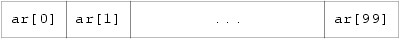
\includegraphics[type=pdf,read=.pdf,ext=.pdf,scale=0.9]{figure/5.1_arr}
     \caption*{Diagram showing an array consisting of elements labelled 'ar[0]',           'ar[1]', etc., up to 'ar[99]'.}
     \caption{\label{fig:arr}100 element array}
   \end{figure*}



  Each of the hundred members is a separate variable whose type is
   \double. Without exception, all arrays in C are numbered from
   \texttt{0} up to one less than the bound given in the declaration.
   This is a prime cause of surprise to beginners--watch out for it. For
   simple examples of the use of arrays, look back at earlier chapters where
   several problems are solved with their help.


  One important point about array declarations is that they don't permit
   the use of varying subscripts. The numbers given must be constant
   expressions which can be evaluated at compile time, not run time. For
   example, this function incorrectly tries to use its argument in the size
   of an array declaration:


  \begin{Verbatim}
    f(int x) {
      char var_sized_array[x];        /* FORBIDDEN */
    }
  \end{Verbatim}

  It's forbidden because the value of x is unknown when the program is
   compiled; it's a run-time, not a compile-time, value.


  To tell the truth, it would be easy to support arrays whose
   \textit{first} dimension is variable, but neither Old C nor the Standard
   permits it, although we do know of one Very Old C compiler that used to
   do it.


  \subsection{Multidimensional arrays}
   

   Multidimensional arrays can be declared like this:


\begin{Verbatim}
int three_dee[5][4][2];
int t_d[2][3];
\end{Verbatim}

   The use of the brackets gives a clue to what is going on. If you refer
   to the precedence table
   given in Section~\ref{subsec:precGrp} (Table~\ref{tab:precAssoc}),
   you'll see that \texttt{[]} associates left to
    right and that, as a result, the first declaration gives us
    a five-element array called three\_dee. The members of that array are
    each a four element array whose members are an array of two ints. We
    have declared arrays of arrays, as Figure~\ref{fig:arr2} shows for two
    dimensions.


    \begin{figure*}\centering
      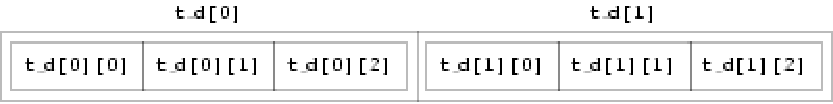
\includegraphics[type=pdf,read=.pdf,ext=.pdf,scale=0.9]{figure/5.2_arr2}
      \caption*{Diagram showing a two dimensional array, with the 'outer' array            having two elements labelled 't\_d[0]' and 't\_d[1]', each with            three elements within it, labelled 't\_d[0][0]', etc.}
     \caption{\label{fig:arr2}Two-dimensional array, showing layout}
   \end{figure*}




   In the diagram, you will notice that \texttt{t\_d[0]} is one
    element, immediately followed by \texttt{t\_d[1]} (there is no
    break).  It so happens that both of those elements are themselves arrays
    of three integers. Because of C's storage layout rules,
    \texttt{t\_d[1][0]} is immediately after \texttt{t\_d[0][2]}. It
    would be possible (but very poor practice) to access
    \texttt{t\_d[1][0]} by making use of the lack of array-bound checking
    in C, and to use the expression \texttt{t\_d[0][3]}. That is not
    recommended--apart from anything else, if the declaration of
    \texttt{t\_d} ever changes, then the results will be likely to
    surprise you.


   That's all very well, but does it really matter in practice? Not much
    it's true; but it is interesting to note that in terms of actual machine
    storage layout the rightmost subscript `varies fastest'. This has
    an impact when arrays are accessed via pointers. Otherwise, they can be
    used just as would be expected; expressions like these are quite in
    order:


   \begin{Verbatim}
three_dee[1][3][1] = 0;
three_dee[4][3][1] += 2;
\end{Verbatim}

   The second of those is interesting for two reasons. First, it accesses
    the very last member of the entire array--although the subscripts
    were declared to be \texttt{[5][4][2]}, the highest usable subscript
    is always one less than the one used in the declaration. Second, it
    shows where the combined assignment operators are a real blessing. For
    the experienced C programmer it is much easier to tell that only one
    array member is being accessed, and that it is being incremented by two.
    Other languages would have to express it like this:


   \begin{Verbatim}
three_dee[4][3][1] = three_dee[4][3][1] + 2;
\end{Verbatim}

   It takes a conscious effort to check that the same array member is
    being referenced on both sides of the assignment. It makes thing easier
    for the compiler too: there is only one array indexing calculation to
    do, and this is likely to result in shorter, faster code. (Of course
    a clever compiler would notice that the left- and right-hand sides look
    alike and would be able to generate equally efficient code--but not
    all compilers are clever and there are lots of special cases where even
    clever compilers are unable to make use of the information.)


   It may be of interest to know that although C offers support for
    multidimensional arrays, they aren't particularly common to see in
    practice. One-dimensional arrays are present in most programs, if for no
    other reason than that's what strings are. Two dimensional arrays are
    seen occasionally, and arrays of higher order than that are most
    uncommon. One of the reasons is that the array is a rather inflexible
    data structure, and the ease of building and manipulating other types of
    data structures in C means that they tend to replace arrays in the more
    advanced programs. We will see more of this when we look at
    pointers.


  

 
        \section{Pointers}
        

  

  Using pointers is a bit like riding a bicycle. Just when you think that
   you'll never understand them--suddenly you do! Once learned the trick
   is hard to forget. There's no real magic to pointers, and a lot of
   readers will already be familiar with their use. The only peculiarity of
   C is how heavily it relies on the use of pointers, compared with other
   languages, and the relatively permissive view of what you can do with
   them.


  \subsection{Declaring pointers}
   

   Of course, just like other variables, you have to declare pointers
    before you can use them. Pointer declarations look much like other
    declarations: but don't be misled. When pointers are declared, the
    keyword at the beginning (c int, char and so on) declares the type of
    variable that the pointer will point to. The pointer itself is not of
    that type, it is of type pointer to that type. A given pointer only
    points to one particular type, not to all possible types. Here's the
    declaration of an array and a pointer:


   \begin{Verbatim}
int ar[5], *ip;
\end{Verbatim}

   We now have an array and a pointer (see Figure~\ref{fig:arrPtr}):


   \begin{figure*}[htb]\centering
     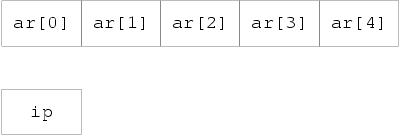
\includegraphics[type=pdf,read=.pdf,ext=.pdf,scale=0.9]{figure/5.3_arrPtr}
     \caption*{Diagram showing an array with four elements
       (labelled 'ar[0]' to 'ar[4]') and a pointer called 'ip'
       which does not currently have any connection to the array.}
     \caption{\label{fig:arrPtr}An array and a pointer}
   \end{figure*}



   The \texttt{*} in front of \texttt{ip} in the declaration
    shows that it is a pointer, not an ordinary variable. It is of type
    \texttt{pointer to int}, and can only be used to refer to variables
    of type int. It's still uninitialized, so to do anything useful with it,
    it has to be made to point to something. You can't just stick some
    integer value into it, because integer values have the type
    \kint, not \texttt{pointer to int}, which is what we
    want.  (In any case, what would it mean if this fragment were valid:


   \begin{Verbatim}
ip = 6;
\end{Verbatim}

   What would \texttt{ip} be pointing to? In fact it could be
    construed to have a number of meanings, but the simple fact is that, in
    C, that sort of thing is just wrong.)


   Here is the right way to initialize a pointer:


   \begin{Verbatim}
int ar[5], *ip;
ip = &ar[3];
\end{Verbatim}

   In that example, the pointer is made to point to the member of the
    array \texttt{ar} whose index is \texttt{3}, i.e. the fourth
    member. This is important. You can assign values to pointers just like
    ordinary variables; the difference is simply in what the value means.
    The values of the variables that we have now
    are shown in Figure~\ref{fig:arrInitPtr} (\texttt{??} means uninitialized).


    \begin{figure*}\centering
      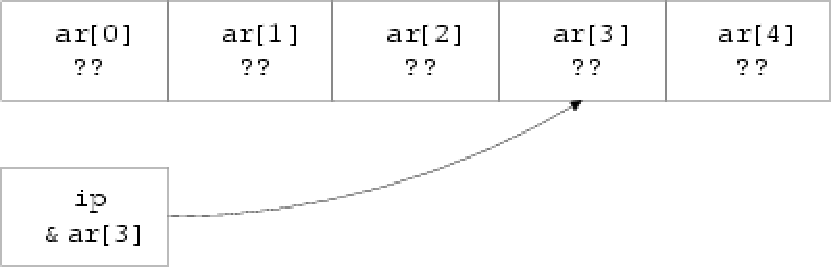
\includegraphics[type=pdf,read=.pdf,ext=.pdf,scale=0.9]
      {figure/5.4_arrInitPtr}
      \caption*{Diagram showing an array with four elements
        (labelled 'ar[0]' to 'ar[4]') each of which has an undefined value,
        and a pointer called 'ip' which contains the address of 'ar[3]'.}
      \caption{\label{fig:arrInitPtr}Array and initialized pointer}
    \end{figure*}



   You can see that the variable \texttt{ip} has the value of the
    expression \texttt{\&ar[3]}. The arrow indicates that, when used
    as a pointer, \texttt{ip} points to the variable
    \texttt{ar[3]}.


   What is this new unary \texttt{\&}? It is usually described as
    the `address-of' operator, since on many systems the pointer will
    hold the store address of the thing that it points to. If you understand
    what addresses are, then you will probably have more trouble than those
    who don't: thinking about pointers as if they were addresses generally
    leads to grief. What seems a perfectly reasonable address manipulation
    on processor X can almost always be shown to be impossible on
    manufacturer Y's washing machine controller which uses 17-bit addressing
    when it's on the spin cycle, and reverses the order of odd and even bits
    when it's out of bleach. (Admittedly, it's unlikely that \textit{anyone}
    could get C to work an an architecture like that. But you should see
    some of the ones it \textit{does} work on; they aren't much better.)


   We will continue to use the term `address of' though, because to
    invent a different one would be even worse.


   Applying the \texttt{\&} operator to an operand returns
    a pointer to the operand:


   \begin{Verbatim}
int i;
float f;
      /* '&i' would be of type pointer to int */
      /* '&f' would be of type pointer to float */
\end{Verbatim}

   In each case the pointer would point to the object named in the
    expression.


   A pointer is only useful if there's some way of getting at the thing
    that it points to; C uses the unary \texttt{*} operator for this
    job.  If \texttt{p} is of type `pointer to something', then *p
    refers to the thing that is being pointed to. For example, to access the
    variable \texttt{x} via the pointer \texttt{p}, this would
    work:


    \VerbatimInput{example/example5-1.c}
    \begin{center}\textit{Example 5.1}\end{center}


   You might be interested to note that, since \texttt{\&} takes
    the address of an object, returning a pointer to it, and since
    \texttt{*} means `the thing pointed to by the pointer', the
    \texttt{\&} and \texttt{*} in the combination
    \texttt{*\&} effectively cancel each other out. (But be careful.
    Some things, constants for example, don't have addresses and the
    \texttt{\&} operator cannot be applied to them;
    \texttt{\&1.5} is not a pointer to anything, it's an error.) It's
    also interesting to see that C is one of the few languages that allows
    an expression on the left-hand side of an assignment operator. Look back
    at the example: the expression \texttt{*p} occurs twice in that
    position, and then the amazing \texttt{(*p)++;} statement. That last
    one is a great puzzle to most beginners--even if you've managed to
    wrap your mind around the concept that \texttt{*p = 0} writes zero
    into the thing pointed to by \texttt{p}, and that \texttt{*p +=
    1} adds one to where \texttt{p} points, it still seems a bit
    much to apply the \pp{} operator to \texttt{*p}.


   The precedence of \texttt{(*p)++} deserves some thought. It will
    be given more later, but for the moment let's work out what happens. The
    brackets ensure that the \texttt * applies to \texttt p,
    so what we have is `post-increment the thing pointed to by \texttt p'.
    Looking at Table~\ref{tab:precAssoc},
    it turns out that \pp{} and \texttt * have equal precedence,
    but they
    associate right to left; in other words, without the brackets, the
    implied operation would have been \texttt{*(p++)},
    whatever that would mean.
    Later on you'll be more used to it--for the moment, we'll be careful
    with brackets to show the way that those expressions work.


   So, provided that a pointer holds the address of something, the
    notation \texttt{*pointer} is equivalent to giving the name of the
    something directly. What benefit do we get from all this? Well, straight
    away it gets round the call-by-value restriction of functions. Imagine
    a function that has to return, say, two integers representing a month
    and a day within that month. The function has some (unspecified) way of
    determining these values; the hard thing to do is to return two separate
    values. Here's a skeleton of the way that it can be done:


    \VerbatimInput{example/example5-2.c}
    \begin{center}\textit{Example 5.2}\end{center}


   Notice carefully the advance declaration of \texttt{date} showing
    that it takes two arguments of type `pointer to \kint{}'.
    It returns \void, because the values are passed back via the
    pointers, not the usual return value. The \texttt{main} function
    passes pointers as arguments to date, which first uses the internal
    variables \texttt{day\_ret} and \texttt{month\_ret} for its
    calculations, then takes those values and assigns them to the places
    pointed to by its arguments.


    When \texttt{date} is called,
    the situation looks like Figure~\ref{fig:callDate}.


   \begin{figure*}[htb]\centering
     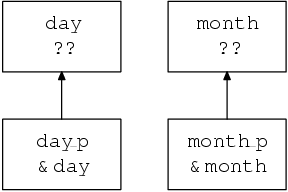
\includegraphics[type=pdf,read=.pdf,ext=.pdf,scale=0.5]
     {figure/5.5_callDate}
     \caption*{Diagram showing the variables 'day' and 'month'
       which have undefined values,
       and the pointers 'day\_p' and 'month\_p' which contain their addresses.}
     \caption{\label{fig:callDate}Just as \texttt\{date\} is called}
   \end{figure*}



   The arguments have been passed to \texttt{date}, but in
    \texttt{main}, day and month are uninitialized. When date reaches
    the return statement,
    the situation is as shown in Figure~\ref{fig:callDateRet}
    (assuming that the values for day and month are 12 and
    5 respectively).


    \begin{figure*}[htb]\centering
      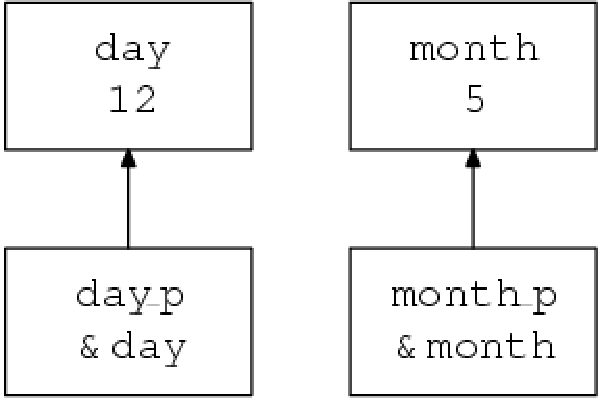
\includegraphics[type=pdf,read=.pdf,ext=.pdf,scale=0.5]
      {figure/5.6_callDateRet}
      \caption*{Diagram showing the same variables as Figure~\ref{fig:callDate},
        except that the 'day' and 'month'
        now have the values '12' and '5' respectively.}
      \caption{\label{fig:callDateRet}
        Just as \texttt\{date\} is about to return}
    \end{figure*}



   One of the great benefits introduced by the new Standard is that it
    allows the types of the arguments to date to be declared in advance.
    A great favourite (and disastrous) mistake in C is to forget that
    a function expects pointers as its arguments, and to pass something else
    instead. Imagine what would have happened if the call of date above had
    read


   \begin{Verbatim}
date(day, month);
\end{Verbatim}

   and no previous declaration of date had been visible. The compiler
    would not have known that date expects pointers as arguments, so it
    would pass the \kint{} values of \texttt{day} and
    \texttt{month} as the arguments. On a large number of computers,
    pointers and integers can be passed in the same way, so the function
    would execute, then pass back its return values by putting them into
    wherever \texttt{day} and \texttt{month} would point if their
    contents were pointers. This is very unlikely to give any sensible
    results, and in general causes unexpected corruption of data elsewhere
    in the computer's store. It can be extremely hard to track down!


   Fortunately, by declaring \texttt{date} in advance, the compiler
    has enough information to warn that a mistake has almost certainly been
    made.


   Perhaps surprisingly, it isn't all that common to see pointers used to
    give this call-by-reference functionality. In the majority of cases,
    call-by-value and a single return value are adequate. What is
    \textit{much} more common is to use pointers to `walk' along
    arrays.


  

  \subsection{Arrays and pointers}\label{subsec:arrPtr}
   

   Array elements are just like other variables: they have addresses.


   \begin{Verbatim}
int ar[20], *ip;

ip = &ar[5];
*ip = 0;        /* equivalent to ar[5] = 0; */
\end{Verbatim}

   The address of \texttt{ar[5]} is put into \texttt{ip}, then
    the place pointed to has zero assigned to it. By itself, this isn't
    particularly exciting. What \textit{is} interesting is the way that
    pointer arithmetic works. Although it's simple, it's one of the
    cornerstones of C.


   Adding an integral value to a pointer results in another pointer of
    the same type. Adding \textit{n} gives a pointer which points n elements
    further along an array than the original pointer did. (Since \textit{n}
    can be negative, subtraction is obviously possible too.) In the example
    above, a statement of the form


   \begin{Verbatim}
*(ip+1) = 0;
\end{Verbatim}

   would set \texttt{ar[6]} to zero, and so on. Again, this is not
    obviously any improvement on `ordinary' ways of accessing an
    array, but the following is.


   \begin{Verbatim}
int ar[20], *ip;

for (ip = &ar[0]; ip < &ar[20]; ip++)
      *ip = 0;
\end{Verbatim}

   That example is a classic fragment of C. A pointer is set to
    point to the start of an array, then, while it still points inside the
    array, array elements are accessed one by one, the pointer incrementing
    between each one. The Standard endorses existing practice by
    guaranteeing that it's permissible to use the \textit{address} of
    \texttt{ar[20]} even though no such element exists. This allows you
    to use it for checks in loops like the one above. The guarantee only
    extends to one element beyond the end of an array and no further.


   Why is the example better than indexing? Well, most arrays are
    accessed sequentially. Very few programming examples actually make use
    of the `random access' feature of arrays. If you do just want
    sequential access, using a pointer can give a worthwhile improvement in
    speed. In terms of the underlying address arithmetic, on most
    architectures it takes one multiplication and one addition to access
    a one-dimensional array through a subscript. Pointers require no
    arithmetic at all--they nearly always hold the store address of the
    object that they refer to. In the example above, the only arithmetic
    that has to be done is in the \for{} loop, where one
    comparison and one addition are done each time round the loop. The
    equivalent, using indexes, would be this:


   \begin{Verbatim}
int ar[20], i;
for (i = 0; i < 20; i++)
      ar[i] = 0;
\end{Verbatim}

   The same amount of arithmetic occurs in the loop statement, but an
    extra address calculation has to be performed for every array
    access.


   Efficiency is not normally an important issue, but here it can be.
    Loops often get traversed a substantial number of times, and every
    microsecond saved in a big loop can matter. It isn't always easy for
    even a smart compiler to recognize that this is the sort of code that
    could be `pointerized' behind the scenes, and to convert from
    indexing (what the programmer wrote) to actually use a pointer in the
    generated code.


   If you have found things easy so far, read on. If not, it's a good
    idea to skip to Section~\ref{subsec:qualTypes}. What follows, while
    interesting, isn't essential. It has been known to frighten even
    experienced C programmers.


   To be honest, C doesn't really `understand' array indexing,
    except in declarations. As far as the compiler is concerned, an
    expression like \texttt{x[n]} is translated into \texttt{*(x+n)}
    and use made of the fact that an array name is converted into a pointer
    to the array's first element whenever the name occurs in an expression.
    That's why, amongst other things, array elements count from zero: if
    \texttt{x} is an array name, then in an expression, \texttt{x}
    is equivalent to \texttt{\&x[0]}, i.e. a pointer to the first
    element of the array. So, since \texttt{*(\&x[0])} uses the
    pointer to get to \texttt{x[0]}, \texttt{*(\&x[0] + 5)} is
    the same as \texttt{*(x + 5)} which is the same as
    \texttt{x[5]}. A curiosity springs out of all this. If
    \texttt{x[5]} is translated into \texttt{*(x + 5)}, and the
    expression \texttt{x + 5} gives the same result as \texttt{5
    + x} (it does), then \texttt{5[x]} should give the identical
    result to \texttt{x[5]}! If you don't believe that, here is
    a program that compiles and runs successfully:


    \VerbatimInput{example/example5-3.c}
    \begin{center}\textit{Example 5.3}\end{center}


   \subsubsection{Summary}
    \begin{itemize}
     \item Arrays always index from zero--end of story.

     \item There are no multidimensional arrays; you use arrays of arrays
      instead.

     \item Pointers point to things; pointers to different types are
      themselves different types. They have nothing in common with each
      other or any other types in C; there are no automatic conversions
      between pointers and other types.

     \item Pointers can be used to simulate `call by reference' to
      functions, but it takes a little work to do it.

     \item Incrementing or adding something to a pointer can be used to step
      along arrays.

     \item To facilitate array access by incrementing pointers, the Standard
      guarantees that in an n element array, although element
      n does not exist, use of its address is not an
      error--the valid range of addresses for an array declared as
      \texttt{int ar[N]} is \texttt{\&ar[0]} through to
      \texttt{\&ar[N]}. You must not try to access this last
      pseudo-element.
    \end{itemize}
   

  

  \subsection{Qualified types}\label{subsec:qualTypes}
   

   If you are confident that you have got a good grasp of the basic
    declaration and use of pointers we can continue. If not, it's important
    to go back over the previous material and make sure that there is
    nothing in it that you still find obscure; although what comes next
    looks more complicated than it really is, there's no need to make it
    worse by starting unprepared.


   The Standard introduces two things called \textbf{type qualifiers},
    neither of which were in Old C. They can be applied to any declared type
    to modify its behaviour--hence the term `qualifier'--and
    although one of them can be ignored for the moment (the one named
    \volatile{}), the other, \const, cannot.


   If a declaration is prefixed with the keyword \const, then
    the thing that is declared is announced to the world as being constant.
    You must not attempt to modify (change the value of) \const{}
    objects, or you get undefined behaviour. Unless you have used some very
    dirty tricks, the compiler will know that the thing you are trying to
    modify is constant, so it can warn you.


   There are two benefits in being able to declare things to be
    \const.


   \begin{enumerate}
    \item It documents the fact that the thing is unmodifiable and the
     compiler helps to check. This is especially reassuring in the case
     of functions which take pointers as arguments. If the declaration
     of a function shows that the arguments are pointers to constant
     objects, then you know that the function is not allowed to change
     them through the pointers.

    \item If the compiler knows that things are constant, it can often do
     increased amounts of optimization or generate better code.
   \end{enumerate}

   Of course, constants are not much use unless you can assign an initial
    value to them. We won't go into the rules about initialization here
    (they are in Chapter~\ref{chap:structTypes}),
    but for the moment just note that
    any declaration can also assign the value of a constant expression to
    the thing being declared. Here are some example declarations involving
    const:


   \begin{Verbatim}
const int x = 1;        /* x is constant */
const float f = 3.5;    /* f is constant */
const char y[10];       /* y is an array of 10 const ints */
                        /* don't think about initializing it yet! */
\end{Verbatim}

   What is more interesting is that pointers can have this qualifier
    applied in two ways: either to the thing that it points to (pointer to
    const), or to the pointer itself (constant pointer). Here are examples
    of \textit{that}:


   \begin{Verbatim}
int i;                  /* i is an ordinary int */
const int ci = 1;       /* ci is a constant int */
int *pi;                /* pi is a pointer to an int */
const int *pci;         /* pci is a pointer to a constant int */
      /* and now the more complicated stuff */

/* cpi is a constant pointer to an int */
int *const cpi = &i;

/* cpci is a constant pointer to an constant int */
const int *const cpci = &ci;
\end{Verbatim}

   The first declaration (of \texttt{i}) is unsurprising. Next, the
    declaration of \texttt{ci} shows that it is a constant integer, and
    therefore may not be modified. If we didn't initialize it, it would be
    pretty well useless.


   It isn't hard to understand what a pointer to an integer and a pointer
    to a constant integer do--but note that they are different types of
    pointer now and can't be freely intermixed. You can change the values of
    both \texttt{pi} and \texttt{pci} (so that they point to other
    things); you can change the value of the thing that \texttt{pi}
    points to (it's not a constant integer), but you are only allowed to
    inspect the value of the thing that \texttt{pci} points to because
    that is a constant.


   The last two declarations are the most complicated. If the pointers
    themselves are constant, then you are not allowed to make them point
    somewhere else--so they need to be initialized, just like
    \texttt{ci}. Independent of the \const{} or other status
    of the pointer itself, naturally the thing that it points to can also be
    \const{} or non-\const, with the appropriate
    constraints on what you can do with it.


   A final piece of clarification: what constitutes a qualified type? In
    the example, \texttt{ci} was clearly of a qualified type, but pci
    was not, since the pointer was not qualified, only the thing that it
    points to. The only things that had qualified type in that list were:
    \texttt{ci}, \texttt{cpi}, and \texttt{cpci}.


   Although the declarations do take some mental gymnastics to
    understand, it just takes a little time to get used to seeing them,
    after which you will find that they seem quite natural. The
    complications come later when we have to explain whether or not you are
    allowed to (say) compare an ordinary pointer with a constant pointer,
    and if so, what does it mean? Most of those rules are `obvious'
    but they do have to be stated.


   Type qualifiers are given a further airing in Chapter~\ref{chap:special}.


  

  \subsection{Pointer arithmetic}
   

   Although a more rigorous description of pointer arithmetic is given
    later, we'll start with an approximate version that will do for the
    moment.


   Not only can you add an integral value to a pointer, but you can also
    compare or subtract two pointers of the same type. They must both point
    into the same array, or the result is undefined. The difference between
    two pointers is defined to be the number of array elements separating
    them; the type of this difference is implementation defined and will be
    one of \short, \kint, or \klong. This
    next example shows how the difference can be calculated and used, but
    before you read it, you need to know an important point.


   \textit{In an expression the name of an array is converted to a pointer to
    the first element of the array}. The only places where that is not
    true are when an array name is used in conjunction with
    \sizeof, when a string is used to initialize an array or
    when the array name is the subject of the address-of operator (unary
    \texttt{\&}). We haven't seen any of those cases yet, they will
    be discussed later. Here's the example.


    \VerbatimInput{example/example5-4.c}
    \begin{center}\textit{Example 5.4}\end{center}


   The pointer \texttt{fp2} is stepped along the array, and the
    difference between its current and original values is printed. To make
    sure that \texttt{printf} isn't handed the wrong type of argument,
    the difference between the two pointers is forced to be of type
    \kint{} by using the cast \texttt{(int)}. That allows for
    machines where the difference between two pointers is specified to be
    long.


   Unfortunately, if the difference does happen to be \klong{}
    and the array is enormous, the last example may give the wrong answers.
    This is a safe version, using a cast to force a long value to be
    passed:


    \VerbatimInput{example/example5-5.c}
    \begin{center}\textit{Example 5.5}\end{center}


  

  \subsection{void, null and dubious pointers}
   

   C is careful to keep track of the type of each pointer and will not in
    general allow you to use pointers of different types in the same
    expression. A pointer to char is a different type of pointer from
    a pointer to \kint{} (say) and you cannot assign one to the
    other, compare them, substitute one for the other as an argument to
    a function .... in fact they may even be stored differently in memory
    and even be of different lengths.


   \textit{Pointers of different types are not the same. There are no
    implicit conversions from one to the other (unlike the arithmetic
    types)}.


   There are a few occasions when you \textit{do} want to be able to
    sidestep some of those restrictions, so what can you do?


   The solution is to use the special type, introduced for this purpose,
    of `pointer to \void{}'. This is one of the Standard's
    invented features: before, it was tacitly assumed that `pointer to
    \kchar' was adequate for the task. This has been
    a reasonably successful assumption, but was a rather untidy thing to do;
    the new solution is both safer and less misleading. There isn't any
    other use for a pointer of that type--\texttt{void *} can't
    actually point to anything--so it improves readability. A pointer of
    type \texttt{void *} can have the value of any other pointer
    assigned to and can, conversely, be assigned to any other pointer. This
    must be used with great care, because you can end up in some heinous
    situations. We'll see it being used safely later with the malloc library
    function.


   You may also on occasion want a pointer that is guaranteed not to
    point to any object--the so-called \textbf{null pointer}. It's
    common practice in C to write routines that return pointers. If, for
    some reason, they can't return a valid pointer (perhaps in case of an
    error), then they will indicate failure by returning a null pointer
    instead. An example could be a table lookup routine, which returns
    a pointer to the object searched for if it is in the table, or a null
    pointer if it is not.


   How do you write a null pointer? There are two ways of doing it and
    both of them are equivalent: either an integral constant with the value
    of \texttt{0} or that value converted to type \texttt{void *} by
    using a cast. Both versions are called the \textbf{null pointer
    constant}. If you assign a null pointer constant to any other
    pointer, or compare it for equality with any other pointer, then it is
    first converted the type of that other pointer (neatly solving any
    problems about type compatibility) and will not appear to have a value
    that is equal to a pointer to any object in the program.


   The only values that can be assigned to pointers apart from 0 are the
    values of other pointers of the same type. However, one of the things
    that makes C a useful replacement for assembly language is that it
    allows you to do the sort of things that most other languages prevent.
    Try this:


   \begin{Verbatim}
int *ip;
ip = (int *)6;
*ip = 0xFF;
\end{Verbatim}

   What does that do? The pointer has been initialized to the value of
    6 (notice the cast to turn an integer 6 into a pointer). This is
    a highly machine-specific operation, and the bit pattern that ends up in
    the pointer is quite possibly nothing like the machine representation of
    6.  After the initialization, hexadecimal \texttt{FF} is written into
    wherever the pointer is pointing. The int at location 6 has had
    \texttt{0xFF} written into it--subject to whatever
    `location 6' means on this particular machine.


   It may or may not make sense to do that sort of thing; C gives you the
    power to express it, it's up to you to get it right. As always, it's
    possible to do things like this by accident, too, and to be
    \textit{very} surprised by the results.


  
        \section{Character handling}
        

  

  C is widely used for character and string handling applications. This
   is odd, in some ways, because the language doesn't really have any
   built-in string handling features. If you're used to languages that know
   about string handling, you will almost certainly find C tedious to begin
   with.


  The standard library contains lots of functions to help with string
   processing but the fact remains that it still feels like hard work. To
   compare two strings you have to call a function instead of using an
   equality operator. There is a bright side to this, though. It means that
   the language isn't burdened by having to support string processing
   directly, which helps to keep it small and less cluttered. What's more,
   once you get your string handling programs working in C, they do tend to
   run very quickly.


  Character handling in C is done by declaring arrays (or allocating them
   dynamically) and moving characters in and out of them `by hand'.
   Here is an example of a program which reads text a line at a time from
   its standard input. If the line consists of the string of characters
   \texttt{stop}, it stops; otherwise it prints the length of the line.
   It uses a technique which is invariably used in C programs; it reads the
   characters into an array and indicates the end of them with an extra
   character whose value is explicitly 0 (zero). It uses the library
   \texttt{strcmp} function to compare two strings.


   \VerbatimInput{example/example5-6.c}
   \begin{center}\textit{Example 5.6}\end{center}


  Once more, the example illustrates some interesting methods used widely
   in C programs. By far the most important is the way that strings are
   represented and manipulated.


  Here is a possible implementation of \texttt{strcmp}, which
   compares two strings for equality and returns zero if they are the same.
   The library function actually does a bit more than that, but the added
   complication can be ignored for the moment. Notice the use of
   \const{} in the argument declarations. This shows that the
   function will not modify the contents of the strings, but just inspects
   them. The definitions of the standard library functions make extensive
   use of this technique.


  \VerbatimInput{example/example5-7.c}\begin{center}\textit{Example 5.7}\end{center}


  \subsection{Strings}
   

   Every C programmer `knows' what a string is. It is an array of
    \kchar{} variables, with the last character in the string
    followed by a null. `But I thought a string was something in double
    quote marks', you cry. You are right, too. In C, a sequence like
    this


   \begin{Verbatim}
"a string"
\end{Verbatim}

   is really a character array. It's the only example in C where you can
    declare something at the point of its use.


   \textit{Be warned}: in Old C, strings were stored just like any other
    character array, and were modifiable. Now, the Standard states that
    although they are are arrays of \kchar, (not \texttt{const
    char}), attempting to modify them results in undefined
    behaviour.


   Whenever a string in quotes is seen, it has two effects: it provides
    a declaration and a substitute for a name. It makes a hidden declaration
    of a char array, whose contents are initialized to the character values
    in the string, followed by a character whose integer value is zero. The
    array has no name. So, apart from the name being present, we have
    a situation like this:


   \begin{Verbatim}
char secret[9];
secret[0] = 'a';
secret[1] = ' ';
secret[2] = 's';
secret[3] = 't';
secret[4] = 'r';
secret[5] = 'i';
secret[6] = 'n';
secret[7] = 'g';
secret[8] = 0;
\end{Verbatim}

   an array of characters, terminated by zero, with character values in
    it. But when it's declared using the string notation, it hasn't got
    a name. How can we use it?


   Whenever C sees a quoted string, the presence of the string itself
    serves as the name of the hidden array--not only is the string an
    implicit sort of declaration, it is as if an array name had been given.
    Now, we all remember that the name of an array is equivalent to giving
    the address of its first element, so what is the type of this?


   \begin{Verbatim}
"a string"
\end{Verbatim}

   It's a pointer of course: a pointer to the first element of the hidden
    unnamed array, which is of type \kchar, so the pointer is of
    type `pointer to \kchar'. The situation is shown in
    Figure~\ref{fig:string}.


    \begin{figure*}[htb]\centering
      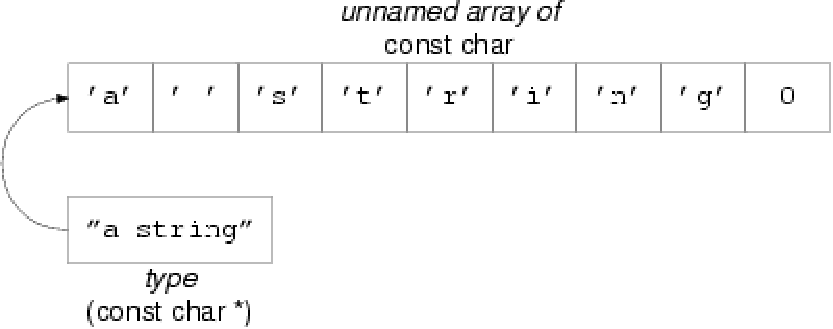
\includegraphics[type=pdf,read=.pdf,ext=.pdf,scale=0.9]
      {figure/5.7_string}
      \caption*{Diagram showing an unnamed array of 'const char' values,
        where the            last item has the value '0',
        and showing that a 'const char *'            value
        that points to the first of them can be used as a string.}
      \caption{\label{fig:string}Effect of using a string}
    \end{figure*}



   For proof of that, look at the following program:


   \verbfilenobox{example/example5-8.c}
   \begin{center}\textit{Example 5.8}\end{center}


   The first loop sets a pointer to the start of the array, then walks
    along until it finds the zero at the end. The second one `knows'
    about the length of the string and is less useful as a result. Notice
    how the first one is independent of the length--that is a most
    important point to remember. It's the way that strings are handled in
    C almost without exception; it's certainly the format that all of the
    library string manipulation functions expect. The zero at the end allows
    string processing routines to find out that they have reached the end of
    the string--look back now to the example function
    \texttt{str\_eq}.  The function takes two character pointers as
    arguments (so a string would be acceptable as one or both arguments). It
    compares them for equality by checking that the strings are
    character-for-character the same. If they are the same at any point,
    then it checks to make sure it hasn't reached the end of them both with
    \texttt{if(*s1 == 0)}: if it has, then it returns 0 to show that
    they were equal. The test could just as easily have been on
    \texttt{*s2}, it wouldn't have made any difference.  Otherwise
    a difference has been detected, so it returns 1 to indicate failure.


   In the example, \texttt{strcmp} is called with two arguments which
    look quite different. One is a character array, the other is a string.
    In fact they're the same thing--a character array terminated by zero
    (the program is careful to put a zero in the first `empty' element
    of \texttt{in\_line}), and a string in quotes--which is
    a character array terminated by a zero. Their use as arguments to strcmp
    results in character pointers being passed, for the reasons explained to
    the point of tedium above.


  

  \subsection{Pointers and increment operators}
   

   We said that we'd eventually revisit expressions like


   \begin{Verbatim}
     (*p)++;
   \end{Verbatim}

   and now it's time. Pointers are used so often to walk down arrays that
    it just seems natural to use the \pp{} and \mm{}
    operators on them. Here we write zeros into an array:


    \verbfilenobox{example/example5-9.c}
    \begin{center}\textit{Example 5.9}\end{center}


   The pointer \texttt{ip} is set to the start of the array. While it
    remains inside the array, the place that it points to has zero written
    into it, then the increment takes effect and the pointer is stepped one
    element along the array. The postfix form of \pp{} is
    particularly useful here.


   This is very common stuff indeed. In most programs you'll find
    pointers and increment operators used together like that, not just once
    or twice, but on almost every line (or so it seems while you find them
    difficult). What is happening, and what combinations can we get? Well,
    the \texttt{*} means indirection, and \pp{} or
    \mm{} mean increment or decrement, respectively;
    either pre- or post-increment.
    The combinations can be pre- or post-increment
    of either the pointer or the thing it points to,
    depending on where the brackets are put.
    Table~\ref{tab:pointerNot} gives a list.


    \begin{table}[htb]
      \centering
      \begin{tabular}{ll}
        \toprule
        \texttt{++(*p)} & pre-increment thing pointed to    \\
        \texttt{(*p)++} & post-increment thing pointed to    \\
        \texttt{*(p++)} & access via pointer, post-increment pointer    \\
        \texttt{*(++p)} & access via pointer which has already been incremented \\
        \bottomrule
      \end{tabular}
      \caption{\label{tab:pointerNot}Pointer notation}
    \end{table}


   Read it carefully; make sure that you understand the combinations.


   The expressions in the list above can usually be understood after
    a bit of head-scratching. Now, given that the precedence of
    \texttt{*}, \pp{} and \mm{} is the same in all
    three cases and that they associate right to left, can you work out what
    happens if the brackets are removed?
    Nasty, isn't it?
    Table~\ref{tab:pointerNot2} shows that there's only one case
    where the brackets have to be there.


    \begin{table}[htb]
      \centering
      \begin{tabular}{ll}
        \toprule
        With parentheses & Without, if possible    \\
        \midrule
        \texttt{++(*p)} & \texttt{++*p}    \\
        \texttt{(*p)++} & \texttt{(*p)++}    \\
        \texttt{*(p++)} & \texttt{*p++}    \\
        \texttt{*(++p)} & \texttt{*++p}    \\
        \bottomrule
      \end{tabular}
      \caption{\label{tab:pointerNot2}More pointer notation}
    \end{table}


   The usual reaction to that horrible sight is to decide that you don't
    care that the parentheses can be removed; you will \textit{always} use
    them in your code. That's all very well but the problem is that most
    C programmers have learnt the important precedence rules (or at least
    learnt the table above) and \textit{they} very rarely put the
    parentheses in. Like them, we don't--so if you want to be able to
    read the rest of the examples, you had better learn to read those
    expressions with or without parentheses. It'll be worth the effort in
    the end.


  

  \subsection{Untyped pointers}
   

   In certain cases it's essential to be able to convert pointers from
    one type to another. This is always done with the aid of casts, in
    expressions like the one below:


   \begin{Verbatim}
(type *) expression
\end{Verbatim}

   The expression is converted into `pointer to
    type', regardless of the expression's previous type. This
    is only supposed to be done if you're sure that you know what you're
    trying to do. It is not a good idea to do much of it until you have got
    plenty of experience. Furthermore, do \textit{not} assume that the cast
    simply suppresses diagnostics of the `mismatched pointer' sort
    from your compiler. On several architectures it is necessary to
    calculate new values when pointer types are changed.


   There are also some occasions when you will want to use
    a `generic' pointer. The most common example is the
    \texttt{malloc} library function, which is used to allocate storage
    for objects that haven't been declared. It is used by telling it how
    much storage is wanted--enough for a \float, or an array
    of \kint, or whatever. It passes back a pointer to enough
    storage, which it allocates in its own mysterious way from a pool of
    free storage (the way that it does this is its own business). That
    pointer is then cast into the right type--for example if
    a \float{} needs 4 bytes of free store, this is the flavour of
    what you would write:


   \begin{Verbatim}
float *fp;

fp = (float *)malloc(4);
\end{Verbatim}

   \texttt{Malloc} finds 4 bytes of store, then the address of that
    piece of storage is cast into pointer-to-float and assigned to the
    pointer.


   What type should \texttt{malloc} be declared to have? The type
    must be able to represent every known value of every type of pointer;
    there is no guarantee that any of the basic types in C can hold such
    a value.


   The solution is to use the \texttt{void *} type that we've already
    talked about. Here is the last example with a declaration of
    \texttt{malloc}:


   \begin{Verbatim}
void *malloc();
float *fp;

fp = (float *)malloc(4);
\end{Verbatim}

   The rules for assignment of pointers show that there is no need to use
    a cast on the return value from \texttt{malloc}, but it is often
    done in practice.


   Obviously there needs to be a way to find out what value the argument
    to \texttt{malloc} should be: it will be different on different
    machines, so you can't just use a constant like 4. That is what the
    \sizeof{} operator is for.


  

 
        \section{Sizeof and storage allocation}
        

  

  The \sizeof{} operator returns the size in bytes of its
   operand. Whether the result of \sizeof{} is \texttt{unsigned
   int} or \texttt{unsigned long} is implementation
   defined--which is why the declaration of malloc above ducked the
   issue by omitting any parameter information; normally you would use the
   \texttt{stdlib.h} header file to declare \texttt{malloc}
   correctly. Here is the last example done portably:


  \begin{Verbatim}
#include <stdlib.h>     /* declares malloc() */
float *fp;

fp = (float *)malloc(sizeof(float));
\end{Verbatim}

  The operand of \sizeof{} only has to be parenthesized if it's
   a type name, as it was in the example. If you are using the name of
   a data object instead, then the parentheses can be omitted, but they
   rarely are.


  \begin{Verbatim}
#include <stdlib.h>

int *ip, ar[100];
ip = (int *)malloc(sizeof ar);
\end{Verbatim}

  In the last example, the array \texttt{ar} is an array of \texttt{100
   ints}; after the call to \texttt{malloc} (assuming that it was
   successful), \texttt{ip} will point to a region of store that can
   also be treated as an array of \texttt{100 ints}.


  The fundamental unit of storage in C is the \kchar, and by
   definition


  \begin{Verbatim}
sizeof(char)
\end{Verbatim}

  is equal to 1, so you could allocate space for an array of ten
   \texttt{char}s with


  \begin{Verbatim}
malloc(10)
\end{Verbatim}

  while to allocate room for an array of ten \kint{}s, you would
   have to use


  \begin{Verbatim}
malloc(sizeof(int[10]))
\end{Verbatim}

  If \texttt{malloc} can't find enough free space to satisfy
   a request it returns a null pointer to indicate failure. For historical
   reasons, the \texttt{stdio.h} header file contains a defined constant
   called NULL which is traditionally used to check the return value from
   \texttt{malloc} and some other library functions. An explicit
   \texttt{0} or \texttt{(void *)0} could equally well be used.


  As a first illustration of the use of \texttt{malloc}, here's
   a program which reads up to \texttt{MAXSTRING} strings from its input
   and sort them into alphabetical order using the library
   \texttt{strcmp} routine. The strings are terminated by
   a `\texttt{\textbackslash n}' character. The sort is done by keeping an array
   of pointers to the strings and simply exchanging the pointers until the
   order is correct. This saves having to copy the strings themselves, which
   improves the efficency somewhat.


  The example is done first using fixed size arrays, then another version
   uses malloc and allocates space for the strings at run time.
   Unfortunately, the array of pointers is still fixed in size: a better
   solution would use a linked list or similar data structure to store the
   pointers and would have no fixed arrays at all. At the moment, we haven't
   seen how to do that.


  The overall structure is this:


  \begin{Verbatim}
while(number of strings read < MAXSTRING
      && input still remains){

              read next string;
}
sort array of pointers;
print array of pointers;
exit;
\end{Verbatim}

  A number of functions are used to implement this program:


  \begin{description}
   \item[\texttt{char *next\_string(char *destination)}] 
    Read a line of characters terminated by `\texttt{$\backslash$n}' from
     the program's input. The first \texttt{MAXLEN-1} characters are
     written into the array pointed to by destination.

    If the first character read is \texttt{EOF}, return a null pointer,
     otherwise return the address of the start of the string (destination).
     On return, destination always points to a null-terminated string.

   

   \item[\texttt{void sort\_arr(const char *p\_array[])}] 
    \texttt{P\_array[]} is an array of pointers to characters. The
     array can be arbitrarily long; its end is indicated by the first element
     containing a null pointer.

    \texttt{Sort\_arr} sorts the pointers so that the pointers point to
     strings which are in alphabetical order when the array is traversed in
     index order.

   

   \item[\texttt{\small void print\_arr(const char *p\_array[])}]
     is like \texttt{sort\_arr}, but prints the strings in index order.
  \end{description}

  It will help to understand the examples if you remember that in an
   expression, an array's name is converted to the address of its first
   element. Similarly, for a two-dimensional array (such as
   \texttt{strings} below), then the expression
   \texttt{strings[1][2]} has type char, but \texttt{strings[1]} has
   type `array of \kchar' which is therefore converted to
   the address of the first element: it is equivalent to
   \texttt{\&strings[1][0]}.


   \VerbatimInput{example/example5-10.c}
   \begin{center}\textit{Example 5.10}\end{center}


  It is no accident that \texttt{next\_string} returns a pointer. We
   can now dispense with the strings array by getting
   \texttt{next\_string} to allocate its own storage.


   \VerbatimInput{example/example5-11.c}
   \begin{center}\textit{Example 5.11}\end{center}


  Finally, for the extremely brave, here is the whole thing with even
   \texttt{p\_array} allocated using \texttt{malloc}. Further, most
   of the array indexing is rewritten to use pointer notation. If you are
   feeling queasy, skip this example. It is hard. One word of explanation:
   \texttt{char **p} means a pointer to a pointer to a character. Many
   C programmers find this hard to deal with.


   \VerbatimInput{example/example5-12.c}
   \begin{center}\textit{Example 5.12}\end{center}


  To further illustrate the use of \texttt{malloc}, another example
   program follows which can cope with arbitrarily long strings. It simply
   reads strings from its standard input, looking for a newline character to
   mark the end of the string, then prints the string on its standard
   output.  It stops when it detects end-of-file. The characters are put
   into an array, the end of the string being indicated (as always) by
   a zero. The newline is not stored, but used to detect when a full line of
   input should be printed on the output. The program doesn't know how long
   the string will be, so it starts by allocating ten characters--enough
   for a short string.


  If the string is more than ten characters long, \texttt{malloc} is
   called to allocate room for the current string plus ten more characters.
   The current characters are copied into the new space, the old storage
   previously allocated is released and the program continues using the new
   storage.


  To release storage allocated by \texttt{malloc}, the library
   function \texttt{free} is used. If you don't release storage when it
   isn't needed any more, it just hangs around taking up space. Using
   \texttt{free} allows it to be `given away', or at least re-used
   later.


  The program reports errors by using \texttt{fprintf}, a close
   cousin of \texttt{printf}. The only difference between them is that
   fprintf takes an additional first argument which indicates where its
   output should go. There are two constants of the right type for this
   purpose defined in \texttt{stdio.h}. Using \texttt{stdout}
   indicates that the program's standard output is to be used;
   \texttt{stderr} refers to the program's standard error stream. On
   some systems both may be the same, but other systems do make the
   distinction.


   \VerbatimInput{example/example5-13.c}
   \begin{center}\textit{Example 5.13}\end{center}


  That may not be a particularly realistic example of how to handle
   arbitrarily long strings--for one thing, the maximum storage demand
   is \textit{twice} the amount needed for the longest string--but it
   does actually work. It also costs rather a lot in terms of copying
   around. Both problems could be reduced by using the library
   \texttt{realloc} function instead.


  A more sophisticated method might use a linked list, implemented with
   the use of \textbf{structures}, as described in the next chapter. That
   would have its drawbacks too though, because then the standard library
   routines wouldn't work for a different method of storing strings.


  \subsection{What sizeof can't do}
   

   One common mistake made by beginners is shown below:


   \VerbatimInput{example/example5-14.c}
   \begin{center}\textit{Example 5.14}\end{center}


   The numbers printed will \textit{not} be the same. The first will,
    correctly, identify the size of \texttt{arr} as \texttt{6}; five
    characters followed by a null. The second one will always, on every
    system, print \texttt{1}. That's because the type of
    \texttt{*cp} is \texttt{const char}, which can only have a size
    of \texttt{1}, whereas the type of \texttt{arr} is different:
    array of \texttt{const char}. The confusion arises because this is
    the one place that the use of an array is not converted into a pointer
    first. It is never possible, using \sizeof, to find out how
    long an array a pointer points to; you \textit{must} have a genuine
    array name instead.


  

  \subsection{The type of sizeof}
   

   Now comes the question of just what this does:


   \begin{Verbatim}
sizeof ( sizeof (anything legal) )
\end{Verbatim}

   That is to say, what type does the result of \sizeof{} have?
    The answer is that it is implementation defined, and will be either
    \texttt{unsigned long} or \texttt{unsigned int}, depending on
    your implementation. There are two safe things to do: either always cast
    the return value to unsigned long, as the examples have done, or to use
    the defined type \texttt{size\_t} provided in the
    \texttt{<stddef.h>} header file. For example:


   \VerbatimInput{example/example5-15.c}\begin{center}\textit{Example 5.15}\end{center}


  

 
        \section{Pointers to functions}
        

  

  A useful technique is the ability to have pointers to functions. Their
   declaration is easy: write the declaration as it would be for the
   function, say


  \begin{Verbatim}
int func(int a, float b);
\end{Verbatim}

  and simply put brackets around the name and a \texttt{*} in front
   of it: that declares the pointer. Because of precedence, if you don't
   parenthesize the name, you declare a function returning a pointer:


  \begin{Verbatim}
/* function returning pointer to int */
int *func(int a, float b);

/* pointer to function returning int */
int (*func)(int a, float b);
\end{Verbatim}

  Once you've got the pointer, you can assign the address of the right
   sort of function just by using its name: like an array, a function name
   is turned into an address when it's used in an expression. You can call
   the function using one of two forms:


  \begin{Verbatim}
(*func)(1,2);
/* or */
func(1,2);
\end{Verbatim}

  The second form has been newly blessed by the Standard. Here's a simple
   example.


   \VerbatimInput{example/example5-16.c}
   \begin{center}\textit{Example 5.16}\end{center}


  If you like writing finite state machines, you might like to know that
   you can have an array of pointers to functions, with declaration and use
   like this:


   \VerbatimInput{example/example5-17.c}
   \begin{center}\textit{Example 5.17}\end{center}


  But we'll draw a veil over it at this point!


 
        \section{Expressions involving pointers}
        

  

  Because of the introduction of qualified types and of the notion of
   incomplete types, together with the use of \texttt{void *}, there are
   now some complicated rules about how you can mix pointers and what
   arithmetic with pointers really permits you to do. Most people will
   survive quite well without ever learning this explicitly, because a lot
   of it is `obvious', but we will include it here in case you do want
   to know. For the final word in accuracy, obviously you will want to see
   what the Standard says. What follows is our interpretation in (hopefully)
   plainer English.


  You don't yet know the Standard means when it talks about
   \textbf{objects} or \textbf{incomplete types}. So far we have tended
   to use the term loosely, but properly speaking an object is a piece of
   data storage whose contents is to be interpreted as a value. A function
   is not an object. An incomplete type is one whose name and type are
   mostly known, but whose size hasn't yet been determined. You can get
   these in two ways:


  \begin{enumerate}
   \item By declaring an array but omitting information about its size:
    \texttt{int x[];}. In that case, there must be additional
    information given later in a definition for the array. The type remains
    incomplete until the later definition.

   \item By declaring a \textbf{structure} or \textbf{union} but not
    defining its contents.  The contents must be defined in a later
    declaration. The type remains incomplete until the later declaration.
  \end{enumerate}

  There will be some more discussion of incomplete types in later
   chapters.


  Now for what you are allowed to do with pointers. Note that wherever we
   talk about qualified types they can be qualified with \const,
   \volatile, or both; the examples are illustrated with const
   only.


  \subsection{Conversions}
   

   Pointers to \void{} can be freely converted backwards and
    forwards with pointers to any object or incomplete type. Converting
    a pointer to an object or an incomplete type to \texttt{void *} and
    then back gives a value which is equal to the original one:


   \begin{Verbatim}
int i;
int *ip;
void *vp;

ip = &i;
vp = ip;
ip = vp;
if (ip != &i)
  printf("Compiler error\n");
\end{Verbatim}

   An unqualified pointer type may be converted to a qualified pointer
    type, but the reverse is not true. The two values will be equal:


   
   \begin{Verbatim}
int i;
int *ip, *const cpi;

ip = &i;
cpi = ip;       /* permitted */
if(cpi != ip)
      printf("Compiler error\n");
ip = cpi;       /* not permitted */
\end{Verbatim}

   A null pointer constant (see earlier) will not be equal to a pointer
    to any object or function.


  

  \subsection{Arithmetic}
   

   Expressions can add (or subtract, which is equivalent to adding
    negative values) integral values to the value of a pointer to any object
    type. The result has the type of the pointer and if n is
    added, then the result points n array elements away from the
    pointer. The most common use is repeatedly to add \texttt{1} to
    a pointer to step it from the start to the end of an array, but addition
    or subtraction of values other than one is possible.


   If the pointer resulting from the addition points in front of the
    array or past the non-existent element just after the last element of
    the array, then you have had overflow or underflow and the result is
    undefined.


   The last-plus-one element of an array has always been assumed to be
    a valid address for a pointer and the Standard confirms this. You
    mustn't actually access that element, but the address is guaranteed to
    exist rather than being an overflow condition.


   We've been careful to use the term `expression' rather than
    saying that you actually add something to the pointer itself. You can do
    that, but only if the pointer is not qualified with \const{}
    (of course). The increment and decrement operators are equivalent to
    adding or subtracting 1.


   Two pointers to \textbf{compatible types} whether or not qualified
    may be subtracted. The result has the type \texttt{ptrdiff\_t}, which
    is defined in the header file \texttt{<stddef.h>}. Both
    pointers must point into the same array, or one past the end of the
    array, otherwise the behaviour is undefined. The value of the result is
    the number of array elements that separate the two pointers. E.g.:


   \begin{Verbatim}
int x[100];
int *pi, *cpi = &x[99]; /* cpi points to the last element of x */

pi = x;
if ((cpi - pi) != 99)
  printf("Error\n");

pi = cpi;
pi++;                   /* increment past end of x */
if ((pi - cpi) != 1)
  printf("Error\n");
\end{Verbatim}

  

  \subsection{Relational expressions}
   

   These allow us to compare pointers with each other. You can only
    compare


   \begin{itemize}
    \item Pointers to compatible object types with each other
    \item Pointers to compatible incomplete types with each other
   \end{itemize}

   It does not matter if the types that are pointed to are qualified or
    unqualified.


   If two pointers compare equal to each other then they point to the
    same thing, whether it is an object or the non-existent element off the
    end of an array (see arithmetic, above). If two pointers point to the
    same thing, then they compare equal to each other. The relational
    operators >, <= and so on all give the result that you would
    expect if the pointers point into the same array: if one pointer
    compares less than another, then it points nearer to the front of the
    array.


   A null pointer constant can be assigned to a pointer; that pointer
    will then compare equal to the null pointer constant (which is pretty
    obvious). A null pointer constant or a null pointer will not compare
    equal to a pointer that points to anything which actually exists.


  

  \subsection{Assignment}
   

   You can use pointers with the assignment operators if the following
    conditions are met:


   \begin{itemize}
    \item The left-hand operand is a pointer and the right-hand operand is a
     null pointer constant.
    \item One operand is a pointer to an object or incomplete type; the other
     is a pointer to \void{} (whether qualified or not).
    \item Both of the operands are pointers to compatible types (whether
     qualified or not).
   \end{itemize}

   In the last two cases, the type pointed to by the left-hand side must
    have at least the same qualifiers as the type pointed to by the
    right-hand side (possibly more).


   So, you can assign a pointer to int to a pointer to \texttt{const
    int} (more qualifiers on the left than the right) but you cannot
    assign a pointer to \texttt{const int} to a pointer to
    \kint. If you think about it, it makes sense.


   The \texttt{+=} and \texttt{-=} operators can involve pointers
    as long as the left-hand side is a pointer to an object and the
    right-hand side is an integral expression. The arithmetic rules above
    describe what happens.


  

  \subsection{Conditional operator}
   

   The description of the behaviour of this operator when it is used with
     pointers has already been given in Chapter~\ref{chap:cntrlFlow}.


  

 
        \section{Summary}
        


  You have been introduced to arrays, pointers and the storage allocater.
   The last of the topics will prove to be more useful in the next chapter,
   but the other two are are central to the language.


  You \textit{cannot} use C properly without understanding the use of
   pointers. Arrays are simple and unsurprising, except for the fact that
   when it's used in an expression, an array name usually converts into
   a pointer to its first element; that often takes time to sink in.


  The C approach to support for strings often causes raised eyebrows. The
   null-terminated array of character model is both powerful and flexible.
   The fact that string manipulation is not built in to the language at
   first glance seems to rule C out of serious contention for
   character-oriented work, yet that is exactly where the language scores
   well compared with the alternatives, at least when speed is important.
   All the same, it's hard work for the programmer.


  Pointer arithmetic is easy and extremely convenient. It's harder for
   ex-assembler programmers to learn, because of the tendency to try to
   translate it into what they `know' the machine is doing. However,
   much harder for people with very low-level experience is the idea of the
   non-equivalence of pointers of different types. Try hard to throw away
   the idea that pointers contain addresses (in the hardware sense) and it
   will repay the effort.


  The facility to obtain arbitrary pieces of storage using
   \texttt{malloc} and the associated stuff is extremely important. You
   might wish to defer it for a while, but don't leave it for too long. An
   obvious feature of C programs written by inexperienced users is their
   dependence on fixed size arrays. \texttt{Malloc} gives you
   considerably more flexibility and is worth the effort to learn about.


  The examples of the use of \sizeof{} should help to eliminate
   a few common misconceptions about what it does. You may not use it all
   that often, but when you do need it, there's no substitute.


 
        \section{Exercises}
        

  \textbf{Exercise 5.1.} What is the valid range of indices for an array of ten
   objects?


  \textbf{Exercise 5.2.} What happens if you take the address of the 11th member
   of that array?


  \textbf{Exercise 5.3.} When is it valid to compare the values of two
   pointers?


  \textbf{Exercise 5.4.} What is the use of a pointer to
   \void{}?


  \textbf{Exercise 5.5.} Write functions which:

\begin{enumerate}
    \item Compare two strings for equality. If they are equal, zero is returned,
     otherwise the difference in value between the first two non-matching
     characters.

    \item Find the first occurrence of a specific character in a given string.
     Return a pointer to the occurrence in the string, or zero if it is not
     found.

    \item Take two strings as arguments. If the first exists in the second as a
     substring, return a pointer to the first occurrence, otherwise zero.
   \end{enumerate}

  \textbf{Exercise 5.6.} Explain the examples using malloc to somebody
   else.


 \chapter{Structured Data Types}\label{chap:structTypes}


        \section{History}
        

  

  The development of the early computer languages went either one way or the
   other. COBOL concentrated on the structure of data but not on arithmetic or
   algorithms, FORTRAN and Algol leant the other way. Scientific users wanted
   to do numeric work on relatively unstructured data (although arrays were
   soon found to be indispensable) and commercial users needed only basic
   arithmetic but knew that the key issue was the structure of the data.


  The ideas that have influenced C are a mixture of the two schools; it has
   the structured control of flow expected in a language of its age, and has
   also made a start on data structures. So far we have concentrated on the
   algorithmic aspects of the language and haven't thought hard about data
   storage. Whilst it's true that arrays fall into the general category of data
   structuring, they are so simple, and so commonly in use, that they don't
   deserve a chapter to themselves. Until now we have been looking at a kind of
   block-structured FORTRAN.


  The trend in the late 1980s and early '90s seems to be towards integrating
   both the data and the algorithms; it's then called Object-Oriented
   programming. There is no specific support for that in C. C++ is a language
   based on C that does offer support for Object-Oriented techniques, but it is
   out of our scope to discuss it further.


  For a large class of problems in computing, it is the data and not the
   algorithms that are the most interesting. If the initial design gets its
   data structures right, the rest of the effort in putting a program together
   is often quite small. However, you need help from the language. If there is
   no support for structured data types other than arrays, writing programs
   becomes both less convenient and also more prone to errors. It is the job of
   a good language to do more than just allow you to do something; it must
   actively \textit{help} as well.


  C offers arrays, structures and unions as its contribution to data
   structuring. They have proved to be entirely adequate for most users' needs
   over the years and remain essentially unchanged by the Standard.


 
        \section{Structures}
        

  

  Arrays allow for a named collection of identical objects. This is suitable
   for a number of tasks, but isn't really very flexible. Most real data
   objects are complicated things with an inherent structure that does not fit
   well on to array style storage. Let's use a concrete example.


  Imagine that the job is something to do with a typesetting package. In
    this system, the individual characters have not only their character values
    but also some additional attributes like font and point size. The font
    doesn't affect the character as such, but only the way that it is
    displayed: this is the normal font, \textit{this is in italics} and this is
    \textbf{in bold font}. Point size is similar. It describes the size of
    the characters when they are printed. For example, the point size of this
    text increases  {\large{now. It goes back again}} now.  If
    our characters have three independent attributes, how can they be
    represented in a single object?


  With C it's easy. First work out how to represent the individual
   attributes in the basic types. Let's assume that we can still store the
   character itself in a char, that the font can be encoded into
   a \short{} (1 for regular, 2 italic, 3 bold etc.) and that the
   point size will also fit a short. These are all quite reasonable
   assumptions.  Most systems only support a few tens of fonts even if they are
   very sophisticated, and point sizes are normally in the range 6 to the small
   hundreds. Below 6 is almost invisible, above 50 is bigger than the biggest
   newspaper banner headlines. So we have a char and two shorts that are to be
   treated as a single entity. Here's how to declare it in C.


  \begin{Verbatim}
struct wp_char {
  char wp_cval;
  short wp_font;
  short wp_psize;
};
\end{Verbatim}

  That effectively declares a new type of object which can be used in your
   program. The whole thing is introduced by the \struct{} keyword,
   which is followed by an optional identifier known as the \texttt{tag},
   \texttt{wp\_char} in this case. The tag only serves the purpose of giving
   a name to this type of structure and allows us to refer to the type later
   on.  After a declaration like the one just seen, the tag can be used like
   this:


  \begin{Verbatim}
struct wp_char x, y;
\end{Verbatim}

  That defines two variables called \texttt{x} and \texttt{y} just
   as it would have done if the definition had been


  \begin{Verbatim}
int x, y;
\end{Verbatim}

  but of course in the first example the variables are of type \texttt{struct
   wp\_char}, and in the second their type is \kint. The tag is
   a name for the new type that we have introduced.


  It's worth remembering that structure tags can safely be used as ordinary
   identifiers as well. They only mean something special when they are preceded
   by the keyword \struct. It is quite common to see a structured
   object being defined with the same name as its structure tag.


  \begin{Verbatim}
struct wp_char wp_char;
\end{Verbatim}

  That defines a variable called \texttt{wp\_char} of type \texttt{struct
   wp\_char}. This is described by saying that structure tags have their
   own `name space' and cannot collide with other names. We'll
   investigate tags some more in the discussion of `incomplete
   types'.


  Variables can also be defined immediately following a structure
   declaration.


  \begin{Verbatim}
struct wp_char {
  char wp_cval;
  short wp_font;
  short wp_psize;
} v1;

struct wp_char v2;
\end{Verbatim}

  We now have two variables, \texttt{v1} and \texttt{v2}. If all the
   necessary objects are defined at the end of the structure declaration, the
   way that \texttt{v1} was, then the tag becomes unneccessary (except if
   it is needed later for use with \sizeof{} and in casts) and is
   often not present.


  The two variables are structured objects, each containing three separate
   \textbf{members} called \texttt{wp\_cval}, \texttt{wp\_font} and
   \texttt{wp\_psize}. To access the individual members of the structures,
   the `dot' operator is used:


  \begin{Verbatim}
v1.wp_cval = 'x';
v1.wp_font = 1;
v1.wp_psize = 10;

v2 = v1;
\end{Verbatim}

  The individual members of \texttt{v1} are initialized to suitable
   values, then the whole of \texttt{v1} is copied into \texttt{v2} in
   an assignment.


  In fact the only operation permitted on whole structures is assignment:
   they can be assigned to each other, passed as arguments to functions and
   returned by functions. However, it is not a very efficient operation to copy
   structures and most programs avoid structure copying by manipulating
   pointers to structures instead. It is generally quicker to copy pointers
   around than structures. A surprising omission from the language is the
   facility to compare structures for equality, but there is a good reason for
   this which will be mentioned shortly.


  Here is an example using an array of structures like the one before.
   A function is used to read characters from the program's standard input and
   return an appropriately initialized structure. When a newline has been read
   or the array is full, the structures are sorted into order depending on the
   character value, and then printed out.


   \VerbatimInput{example/example6-1.c}
   \begin{center}\textit{Example 6.1}\end{center}


  Once it is possible to declare structures it seems pretty natural to
   declare arrays of them, use them as members of other structures and so on.
   In fact the only restriction is that a structure cannot contain an example
   of itself as a member--in which case its size would be an interesting
   concept for philosophers to debate, but hardly useful to a C programmer.


  \subsection{Pointers and structures}
   

   If what the last paragraph says is true--that it is more common to
    use pointers to structures than to use the structures directly--we need
    to know how to do it. Declaring pointers is easy of course:


   \begin{Verbatim}
struct wp_char *wp_p;
\end{Verbatim}

   gives us one straight away. But how do we access the members of the
    structure? One way might be to look through the pointer to get the whole
    structure, then select the member:


   \begin{Verbatim}
/* get the structure, then select a member */
(*wp_p).wp_cval
\end{Verbatim}

   that would certainly work (the parentheses are there because . has
    a higher precedence than \texttt{*}). It's not an easy notation to work
    with though, so C introduces a new operator to clean things up; it is
    usually known as the `pointing-to' operator. Here it is being
    used:


   \begin{Verbatim}
/* the wp_cval in the structure wp_p points to */
wp_p->wp_cval = 'x';
\end{Verbatim}

   and although it might not look a lot easier than its alternative, it pays
    off when the structure contains pointers, as in a linked list. The
    pointing-to syntax is much easier if you want to follow two or three stages
    down the links of a linked list. If you haven't come across linked lists
    before, you're going to learn a lot more than just the use of structures
    before this chapter finishes!


   If the thing on the left of the \texttt{.} or \texttt{->}
    operator is qualified (with \const{} or \volatile{})
    then the result is also has those qualifiers associated with it. Here it
    is, illustrated with pointers; when the pointer points to a qualified type
    the result that you get is also qualified:


   \begin{Verbatim}
#include <stdio.h>
#include <stdlib.h>

struct somestruct{
  int i;
};

main() {
  struct somestruct *ssp, s_item;
  const struct somestruct *cssp;

  s_item.i = 1;   /* fine */
  ssp = &s_item;
  ssp->i += 2;    /* fine */
  cssp = &s_item;
  cssp->i = 0;    /* not permitted - cssp points to const objects */

  exit(EXIT_SUCCESS);
}
\end{Verbatim}

   Not all compiler writers seem to have noticed that requirement--the
    compiler that we used to test the last example failed to warn that the
    final assignment violated a constraint.


   Here is the Example 6.1 rewritten using pointers, and with
    the input function infun changed to accept a pointer to a structure rather
    than returning one. This is much more likely to be what would be seen in
    practice.


   (It is fair to say that, for a really efficient implementation, even the
    copying of structures would probably be dropped, especially if they were
    large. Instead, an array of pointers would be used, and the pointers
    exchanged until the sorted data could be found by traversing the pointer
    array in index order. That would complicate things too much for a simple
    example.)


   \VerbatimInput{example/example6-2.c}\begin{center}\textit{Example 6.2}\end{center}


   The next issue is to consider what a structure looks like in terms of
    storage layout. It's best not to worry about this too much, but it is
    sometimes useful if you have to use C to access record-structured data
    written by other programs. The \texttt{wp\_char} structure will be
    allocated storage as shown in Figure~\ref{fig:struct}.


    \begin{figure*}[htb]+\centering
      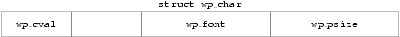
\includegraphics[type=pdf,read=.pdf,ext=.pdf,scale=0.95]
      {figure/6.1_struct}
      \caption*{Diagram showing the layout of the values in 'struct wp\_char',
        with boxes containing 'wp\_cval',
        an empty space of padding, 'wp\_font' and 'wp\_psize'.}
      \caption{\label{fig:struct}Storage Layout of a Structure}
   \end{figure*}



   The diagram assumes a number of things: that a \kchar{} takes
    1 byte of storage; that a \short{} needs 2 bytes; and that
    \short{}s must be aligned on even byte addresses in this
    architecture. As a result the structure contains an unnamed 1-byte member
    inserted by the compiler for architectural reasons. Such addressing
    restrictions are quite common and can often result in structures containing
    `holes'.


   The Standard makes some guarantees about the layout of structures and
    unions:


   \begin{itemize}
    \item Members of a structure are allocated within the structure in the
     order of their appearance in the declaration and have ascending
     addresses.

    \item There must not be any padding in front of the first member.

    \item The address of a structure is the same as the address of its first
     member, provided that the appropriate cast is used. Given the
     previous declaration of \texttt{struct wp\_char}, if item is of type
     \texttt{struct wp\_char}, then
     \texttt{(char *)item == \&item.wp\_cval}.

    \item Bit fields (see Section~\ref{sec:bitfields}) don't actually have
     addresses, but are conceptually packed into \textbf{units} which obey
     the rules above.
   \end{itemize}

  

  \subsection{Linked lists and other structures}
   

   The combination of structures and pointers opens up a lot of interesting
    possibilities. This is not a textbook on complex linked data structures,
    but it will go on to describe two very common examples of the breed: linked
    lists and trees. Both have a feature in common: they consist of structures
    containing pointers to other structures, all the structures typically being
    of the same type. Figure~\ref{fig:linkedList} shows a picture of a linked
    list.


    \begin{figure*}[htb]\centering
      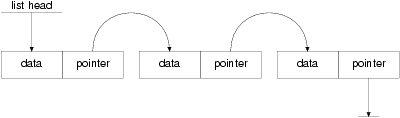
\includegraphics[type=pdf,read=.pdf,ext=.pdf,scale=0.8]
      {figure/6.2_linkedList}
      \caption*{Diagram showing a linked list of three items,
        with a pointer  labelled 'list head' pointing to the first item,
        and each item containing a 'data' value and a 'pointer' value
        which points to the next item (the last pointer is null).}
      \caption{\label{fig:linkedList}List linked by pointers}
   \end{figure*}



   The sort of declaration needed for that is this:


   \begin{Verbatim}
struct list_ele {
  int data;       /* or whatever you like here */
  struct list_ele *ele_p;
};
\end{Verbatim}

   Now, at first glance, it seems to contain itself--which is
    forbidden--but in fact it only contains a \textit{pointer} to itself.
    How come the pointer declaration is allowed? Well, by the time the compiler
    reaches the pointer declaration it already knows that there is such a thing
    as a \texttt{struct list\_ele} so the declaration is permitted. In fact,
    it is possible to make an incomplete declaration of a structure by
    saying


   \begin{Verbatim}
struct list_ele;
\end{Verbatim}

   at some point before the full declaration. A declaration like that
    declares an \textbf{incomplete type}. This will allow the declaration of
    pointers before the full declaration is seen. It is also important in the
    case of cross-referencing structures where each must contain a pointer to
    the other, as shown in the following example.


    \VerbatimInput{example/example6-3.c}
    \begin{center}\textit{Example 6.3}\end{center}


   This illustrates the need for incomplete types. It also illustrates an
    important thing about the names of structure members: they inhabit
    a name-space per structure, so element names can be the same in different
    structures without causing any problems.


   Incomplete types may only be used where the size of the structure isn't
    needed yet. A full declaration must have been given by the time that the
    size is used. The later full declaration mustn't be in an inner block
    because then it becomes a new declaration of a different structure.


    \VerbatimInput{example/example6-4.c}
    \begin{center}\textit{Example 6.4}\end{center}


   There's one thing to watch out for: you get a incomplete type of
    a structure \textit{simply by mentioning its name!} That means that this
    works:


   \begin{Verbatim}
struct abc { struct xyz *p;};
      /* the incomplete type 'struct xyz' now declared */
struct xyz { struct abc *p;};
      /* the incomplete type is now completed */
\end{Verbatim}

   There's a horrible danger in the last example, though, as this shows:


   \begin{Verbatim}
struct xyz {float x;} var1;

main() {
  struct abc{ struct xyz *p;} var2;

  /* AAAGH - struct xyz REDECLARED */
  struct xyz{ struct abc *p;} var3;
}
\end{Verbatim}

   The result is that \texttt{var2.p} can hold the address of
    \texttt{var1}, but emphatically not the address of \texttt{var3}
    which is of a different type! It can be fixed (assuming that it's not what
    you wanted) like this:


   \begin{Verbatim}
struct xyz{float x;} var1;

main(){
      struct xyz;     /* new incomplete type 'struct xyz' */
      struct abc{ struct xyz *p;} var2;
      struct xyz{ struct abc *p;} var3;
}
\end{Verbatim}

   The type of a structure or union is completed when the closing \texttt{\}} of its
    declaration is seen; it must contain at least one member or the behaviour
    is undefined.


   The other principal way to get incomplete types is to declare arrays
    without specifying their size--their type is incomplete until a later
    declaration provides the missing information:


   \begin{Verbatim}
int ar[];       /* incomplete type */
int ar[5];      /* completes the type */
\end{Verbatim}

   If you try that out, it will only work if the declarations are outside
    any blocks (external declarations), but that's for other reasons.


   Back to the linked list. There were three elements linked into the list,
    which could have been built like this:


    \VerbatimInput{example/example6-5.c}
    \begin{center}\textit{Example 6.5}\end{center}


   and the contents of the list can be printed in two ways. The array can be
    traversed in order of index, or the pointers can be used as in the
    following example.


    \VerbatimInput{example/example6-6.c}
    \begin{center}\textit{Example 6.6}\end{center}


   It's the way that the pointers are followed which makes the example
    interesting. Notice how the pointer in each element is used to refer to the
    next one, until the pointer whose value is \texttt{0} is found. That
    value causes the \while{} loop to stop. Of course the pointers
    can be arranged in any order at all, which is what makes the list such
    a flexible structure. Here is a function which could be included as part of
    the last program to sort the linked list into numeric order of its data
    fields. It rearranges the pointers so that the list, when traversed in
    pointer sequence, is found to be in order. It is important to note that the
    data itself is not copied. The function must return a pointer to the head
    of the list, because that is not necessarily at \texttt{ar[0]} any
    more.


    \VerbatimInput{example/example6-7.c}
    \begin{center}\textit{Example 6.7}\end{center}


   Expressions such as \texttt{thisp->pointer->pointer} are
    commonplace in list processing. It's worth making sure that you understand
    it; the notation emphasizes the way that links are followed.


  

  \subsection{Trees}
   

   Another very popular data structure is the tree. It's actually a linked
    list with branches; a common type is the \textbf{binary tree} which has
    elements (\texttt{nodes}) looking like this:


   \begin{Verbatim}
struct tree_node {
  int data;
  struct tree_node *left_p, *right_p;
};
\end{Verbatim}

   For historical and essentially irrelevant reasons, trees in computer
    science work upside down. They have their \textbf{root} node at the top
    and their \textbf{branches} spread out downwards.
    In Figure~\ref{fig:tree},
    the `data' members of the nodes are replaced by values
    which will be used in the discussion that follows.


    \begin{figure*}[htb]\centering
      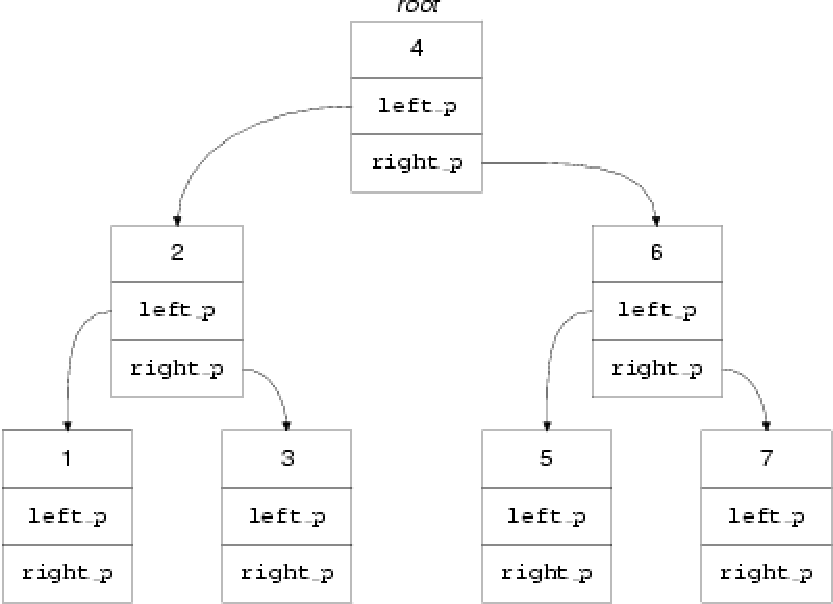
\includegraphics[type=pdf,read=.pdf,ext=.pdf,scale=0.8]
      {figure/6.3_tree}
      \caption*{A tree structure, made up of 7 items,
        each of which is labelled with a different number.
        Each item has two pointer values, labelled 'left\_p' and 'right\_p',
        which point to child items.
        One item is labelled 'root'
        and isn't a child of any of the other  items.}
      \caption{\label{fig:tree}A tree}
    \end{figure*}



   Trees may not seem very exciting if your main interest lies in routine
    character handling and processing, but they are extremely important to the
    designers of databases, compilers and other complex tools.


   The advantage of a tree is that, if it is properly arranged, the layout
    of the data can support binary searching very simply. It is always possible
    to add new nodes to a tree at the appropriate place and a tree is basically
    a flexible and useful data structure.


   Look at Figure~\ref{fig:tree}. The tree is carefully constructed so
    that it can be searched to find whether a given value can be found in the
    data portions of the nodes. Let's say we want to find if a value
    x is already present in the tree. The algorithm is this:


   \begin{Verbatim}
Start at the root of the tree:
if the tree is empty (no nodes)
        then return `failure'.
else if the data in the current node is equal
        to the value being searched for
        then return `success'.
else if the data in the current node is greater than the
        value being searched for
        then search the tree indicated by the left pointer
else search the tree indicated by the right pointer.
\end{Verbatim}

   Here it is in C:


   \VerbatimInput{example/example6-8.c}
   \begin{center}\textit{Example 6.8}\end{center}


   So that works fine. It is also interesting to note that, given a value,
    it can always be inserted at the appropriate point in the tree. The same
    search algorithm is used, but, instead of giving up when it finds that the
    value is not already in the tree, a new node is allocated by
    \texttt{malloc}, and is hung on the tree at the very place where the
    first null pointer was found. This is a mite more complicated to do because
    of the problem of handling the root pointer itself, and so a pointer to
    a pointer is used. Read the example carefully; it is not likely that you
    ever find anything more complicated than this in practice. If you can
    understand it, there is not much that should worry you about the vast
    majority of C language programs.


    \VerbatimInput{example/example6-9.c}
    \begin{center}\textit{Example 6.9}\end{center}


   Finally, the algorithm that allows you to walk along the tree visiting
    all the nodes in order is beautiful. It is the cleanest example of
    recursion that you are likely to see. Look at it and work out what it
    does.


    \VerbatimInput{example/example6-10.c}
    \begin{center}\textit{Example 6.10}\end{center}


  

 
        \section{Unions}
        

  

  Unions don't take long to explain. They are the same as structures, except
   that, where you would have written \struct{} before, now you write
   \union. Everything works the same way, but with one big
   exception. In a structure, the members are allocated separate consecutive
   chunks of storage. In a union, every member is allocated the same piece of
   storage. What would you use them for? Well, sometimes you want a structure
   to contain different values of different types at different times but to
   conserve space as much as possible. Using a union, it's up to you to keep
   track of whatever type you put into it and make sure that you retrieve the
   right type at the right time. Here's an example:


   \VerbatimInput{example/example6-11.c}
   \begin{center}\textit{Example 6.11}\end{center}


  If the example had, say, put a \float{} into the union and then
   extracted it as an int, a strange value would have resulted. The two types
   are almost certainly not only stored differently, but of different lengths.
   The \kint{} retrieved would probably be the low-order bits of the
   machine representation of a \float, and might easily be made up
   of part of the mantissa of the \float{} plus a piece of the
   exponent. The Standard says that if you do this, the behaviour is
   implementation defined (not undefined). The behaviour is defined by the
   Standard in one case: if some of the members of a union are structures with
   a `common initial sequence' (the first members of each structure have
   compatible type and in the case of \textbf{bitfields} are the same
   length), and the union currently contains one of them, then the common
   initial part of each can be used interchangeably. Oh good.


  The C compiler does no more than work out what the biggest member in
   a union can be and allocates enough storage (appropriately aligned if
   neccessary). In particular, no checking is done to make sure that the right
   sort of use is made of the members. That is your task, and you'll soon find
   out if you get it wrong. The members of a union all start at the same
   address--there is guaranteed to be no padding in front of any of
   them.


  The most common way of remembering what is in a union is to embed it in
   a structure, with another member of the structure used to indicate the type
   of thing currently in the union. Here is how it might be used:


   \VerbatimInput{example/example6-12.c}
   \begin{center}\textit{Example 6.12}\end{center}


  That also demonstrates how the dot notation is used to access structures
   or unions inside other structures or unions. Some current C compilers allow
   you to miss bits out of the names of embedded objects provided that they are
   not ambiguous. In the example, such an unambiguous name would be
   \texttt{var\_type.un\_int} and the compiler would work out what you meant.
   None the less this is not permitted by the Standard.


  It is because of unions that structures cannot be compared for equality.
   The possibility that a structure might contain a union makes it hard to
   compare such structures; the compiler can't tell what the union currently
   contains and so wouldn't know how to compare the structures. This sounds
   a bit hard to swallow and isn't 100\% true--most structures don't contain
   unions--but there is also a philosophical issue at stake about just what
   is meant by `equality' when applied to structures. Anyhow, the union
   business gives the Standard a good excuse to avoid the issue by not
   supporting structure comparison.


 
        \section{Bitfields}\label{sec:bitfields}
        

  

  While we're on the subject of structures, we might as well look at
   bitfields. They can only be declared inside a structure or a union, and
   allow you to specify some very small objects of a given number of bits in
   length.  Their usefulness is limited and they aren't seen in many programs,
   but we'll deal with them anyway. This example should help to make things
   clear:


   \VerbatimInput{example/example6-13.c}
   \begin{center}\textit{Example 6.13}\end{center}


  Each field is accessed and manipulated as if it were an ordinary member of
   a structure. The keywords \signed{} and \unsigned{} mean
   what you would expect, except that it is interesting to note that a 1-bit
   signed field on a two's complement machine can only take the values
   \texttt{0} or \texttt{-1}. The declarations are permitted to include
   the \const{} and \volatile{} qualifiers.


  The main use of bitfields is either to allow tight packing of data or to
   be able to specify the fields within some externally produced data files.
   C gives no guarantee of the ordering of fields within machine words, so if
   you do use them for the latter reason, you program will not only be
   non-portable, it will be compiler-dependent too. The Standard says that
   fields are packed into `storage units', which are typically machine
   words. The packing order, and whether or not a bitfield may cross a storage
   unit boundary, are implementation defined. To force alignment to a storage
   unit boundary, a zero width field is used before the one that you want to
   have aligned.


  Be careful using them. It can require a surprising amount of run-time code
   to manipulate these things and you can end up using more space than they
   save.


  Bit fields do not have addresses--you can't have pointers to them or
   arrays of them.


 
        \section{Enums}
        

  

  These fall into the category of `half baked'. They aren't proper
   enumerated types, as in Pascal, and only really serve to help you reduce the
   number of \texttt{\#define} statements in your program. They look like
   this:


  \begin{Verbatim}
enum e_tag{
  a, b, c, d=20, e, f, g=20, h
} var;
\end{Verbatim}

  Just as with structures and unions, the \texttt{e\_tag} is the tag, and
   \texttt{var} is the definition of a variable.


  The names declared inside the enumeration are constants with
   \kint{} type. Their values are these:


  \begin{Verbatim}
a == 0
b == 1
c == 2
d == 20
e == 21
f == 22
g == 20
h == 21
\end{Verbatim}

  so you can see that, in the absence of anything to the contrary, the
   values assigned start at zero and increase. A specific value can be given if
   you want, when the increase will continue one at a time afterwards; the
   specific value must be an \textbf{integral constant} (see later) that is
   representable in an int. It is possible for more than one of the names to
   have the same value.


  The only use for these things is to give a better-scoped version of
   this:


  \begin{Verbatim}
#define a 0
#define b 1
/* and so on */
\end{Verbatim}

  It's better scoped because the declaration of enumerations follows the
   standard scope rules for C, whereas \texttt{\#define} statements have
   file scope.


  Not that you are likely to care, but the Standard states that enumeration
   types are of a type that is compatible with an implementation-defined one of
   the integral types. So what? For interest's sake here is an
   illustration:


  \begin{Verbatim}
enum ee{a,b,c} e_var, *ep;
\end{Verbatim}

  The names \texttt{a}, \texttt{b}, and \texttt{c} all behave as
   if they were \kint{} constants when you use them;
   \texttt{e\_var} has type \texttt{enum ee} and \texttt{ep} is
   a pointer to enum \texttt{ee}. The compatibility requirement means that
   (amongst other implications) there will be an integral type whose address
   can be assigned to \texttt{ep} without violating the type-compatibility
   requirements for pointers.


 
        \section{Qualifiers and derived types}
        

  

  Arrays, structures and unions are `derived from' (contain) other
   types; none of them may be derived from incomplete types. This means that
   a structure or union cannot contain an example of itself, because its own
   type is incomplete until the declaration is complete. Since a pointer to an
   incomplete type is not itself an incomplete type, it \textit{can} be used in
   the derivation of arrays, structures and unions.


  If any of the types that these things are derived from are qualified with
   \const{} or \volatile, they do \textit{not} inherit
   that qualification. This means that if a structure contains
   a \const{} object, the structure itself is not qualified with
   const and any non-const members can still be modified. This is what you
   would expect. However, the Standard does says that if any derived type
   contains a type that is qualified with \const{} (or recursively
   any inner type does) then it is not modifiable--so a structure that
   contains a const cannot be on the left-hand side of an assignment
   operator.


 
        \section{Initialization}
        

  

  Now that we have seen all of the data types supported by C, we can look at
   the subject of initialization. C allows ordinary variables, structures,
   unions and arrays to be given initial values in their definitions. Old C had
   some strange rules about this, reflecting an unwillingness by compiler
   writers to work too hard. The Standard has rationalized this, and now it is
   possible to initialize things as and when you want.


  There are basically two sorts of initialization: at compile time, and at
   run time. Which one you get depends on the \textbf{storage duration} of
   the thing being initialized.


  Objects with \textbf{static duration} are declared either outside
   functions, or inside them with the keyword \extern{} or
   \static{} as part of the declaration. These can \textit{only} be
   initialized at compile time.


  Any other object has \textbf{automatic duration}, and can only be
   initialized at run time. The two categories are mutually exclusive.


   Although they are related,
   storage duration and \textbf{linkage} (see Chapter~\ref{chap:funcs})
   are different and should not be confused.


  Compile-time initialization can only be done using \textbf{constant
   expressions}; run-time initialization can be done using \textit{any}
   expression at all. The Old C restriction, that only simple variables (not
   arrays, structures or unions) could be initialized at run time, has been
   lifted.


  \subsection{Constant expressions}
   

   There are a number of places where constant expressions must be used. The
    definition of what constitutes a constant expression is relatively
    simple.


   A \textbf{constant expression} is evaluated by the compiler, not at
    run-time. It may be used anywhere that a constant may be used. Unless it is
    part of the operand of \sizeof, it may not contain any
    assignment, increment or decrement operations, function calls or comma
    operators; that may seem odd, but it's because \sizeof{} only
    needs to evaluate the type of an expression, not its value.


   If real numbers are evaluated at compile-time, then the Standard insists
    that they are evaluated with at least as much precision and range as will
    be used at run-time.


   A more restricted form, called the \textbf{integral constant
    expression} exists. This has integral type and only involves operands
    that are integer constants, enumeration constants, character constants,
    \sizeof{} expressions and real constants that are the immediate
    operands of casts. Any cast operators are only allowed to convert
    arithmetic types to integral types. As with the previous note on
    \sizeof{} expressions, since they don't have to be evaluated,
    just their type determined, no restrictions apply to their contents.


   The \textbf{arithmetic constant expression} is like the integral
    constant expression, but allows real constants to be used and restricts the
    use of casts to converting one arithmetic type to another.


   The \textbf{address constant} is a pointer to an object that has static
    storage duration or a pointer to a function. You can get these by using the
    \texttt{\&} operator or through the usual conversions of array and
    function names into pointers when they are used in expressions. The
    operators \texttt{[]}, \texttt{.}, \texttt{->},
    \texttt{\&} (address of) and \texttt{*} (pointer dereference) as
    well as casts of pointers can all be used in the expression as long as they
    don't involve accessing the value of any object.


  

  \subsection{More initialization}
   

   The various types of constants are permitted in various places; integral
    constant expressions are particularly important because they are the only
    type of expression that may be used to specify the size of arrays and the
    values in \case{} statement prefixes. The types of constants that
    are permitted in initializer expressions are less restricted; you are
    allowed to use: arithmetic constant expressions; null pointer or address
    constants; an address constant for an object plus or minus an integral
    constant expression. Of course it depends on the type of thing being
    initialized whether or not a particular type of constant expression is
    appropriate.


   Here is an example using several initialized variables:


   \VerbatimInput{example/example6-14.c}\begin{center}\textit{Example 6.14}\end{center}


   Initializing ordinary variables is easy: put \texttt{= expression}
    after the variable name in a declaration, and the variable is initialized
    to the value of the expression. As with all objects, whether you can use
    any expression, or just a constant expression, depends on its storage
    duration.


   Initializing arrays is easy for one-dimensional arrays. Just put a list
    of the values you want, separated by commas, inside curly brackets. The
    example shows how to do it. If you don't give a size for the array, then
    the number of initializers will determine the size. If you do give a size,
    then there must be at most that many initializers in the list. Too many is
    an error, too few will just initialize the first elements of the array.


   You could build up a string like this:


   \begin{Verbatim}
char str[] = {'h', 'e', 'l', 'l', 'o', 0};
\end{Verbatim}

   but because it is so often necessary to do that, it is also permitted to
    use a quoted string literal to initialize an array of chars:


   \begin{Verbatim}
char str[] = "hello";
\end{Verbatim}

   In that case, the null at the end of the string will also be included if
    there is room, or if no size was specified. Here are examples:


   \begin{Verbatim}
/* no room for the null */
char str[5] = "hello";

/* room for the null */
char str[6] = "hello";
\end{Verbatim}

   The example program used string literals for a different purpose:
    \textit{there} they were being used to initialize an array of character
    pointers; a very different prospect.


   For structures that have automatic duration, an expression of the right
    type can be used to initialize them, or else a bracketed list of constant
    expressions must be used:


    \VerbatimInput{example/example6-15.c}
    \begin{center}\textit{Example 6.15}\end{center}


   Only the first member of a union can be initialized.


   If a structure or union contains unnamed members, whether unnamed
    bitfields or padding for alignment, they are ignored in the initialization
    process; they don't have to be counted when you provide the initializers
    for the real members of the structure.


   For objects that contain sub-objects within them, there are two ways of
    writing the initializer. It can be written out with an initializer for each
    member:


    \VerbatimInput{example/example6-16.c}
    \begin{center}\textit{Example 6.16}\end{center}


   which will assign \texttt{1} to \texttt{x[0].a}, \texttt{2}
    to \texttt{x[0].e.c}, \texttt{a} to \texttt{x[0].e.d} and
    \texttt{3} to \texttt{x[1].a} and so on.


   It is \textit{much} safer to use internal braces to show what you mean,
    or one missed value will cause havoc.


    \VerbatimInput{example/example6-17.c}
    \begin{center}\textit{Example 6.17}\end{center}


   \textit{Always} fully bracket initializers--that is much the safest
    thing to do.


   It is the same for arrays as for structures:


   \VerbatimInput{example/example6-18.c}
   \begin{center}\textit{Example 6.18}\end{center}


   that gives full initialization to the first three rows of \texttt{y}.
    The fourth row, \texttt{y[3]}, is uninitialized.


   Unless they have an explicit initializer, all objects with static
    duration are given implicit initializers--the effect is as if the
    constant \texttt{0} had been assigned to their components. This is in
    fact widely used--it is an assumption made by most C programs that
    external objects and internal static objects start with the value zero.


   Initialization of objects with automatic duration is only guaranteed if
    their compound statement is entered `at the top'. Jumping into the
    middle of one may result in the initialization not happening--this is
    often undesirable and should be avoided. It is explicitly noted by the
    Standard with regard to \switch{} statements, where providing
    initializers in declarations \textit{cannot} be of any use; this is because
    a declaration is not linguistically a `statement' and only statements
    may be labelled. As a result it is not possible for initializers in
    \switch{} statements ever to be executed, because the entry to
    the block containing them \textit{must} be below the declarations!


   A declaration inside a function (block scope) can, using various
   techniques
   outlined in Chapter~\ref{chap:funcs} and Chapter~\ref{chap:special},
    be made to refer to an object that has either \textbf{external} or
    \textbf{internal linkage}. If you've managed to do that, and it's not
    likely to happen by accident, then you can't initialize the object as part
    of that declaration. Here is one way of trying it:


   \begin{Verbatim}
int x;                   /* external linkage */
main() {
 extern int x = 5;       /* forbidden */
}
\end{Verbatim}

   Our test compiler didn't notice that one, either.


  

 
        \section{Summary}
        


  You now understand structures and unions. Bitfields and enumeration types
   really are not very important and you could manage quite well without
   them.


  It is hard to emphasize how important is the use of structures, pointers
   and malloc in serious programs. If you aren't familiar with the use of
   structured data in the form of lists, trees and so on, get a good book now.
   Better still, try to enrol on a good course. Except in very specialized
   applications, it is usually the ability to structure data well, not the
   ability to write complicated algorithms, that makes it possible to construct
   clean, small and maintainable programs. Experienced software designers often
   say that once the right structure of the data has been determined, the rest
   is `simple'.


  Undoubtedly, one of the reasons for the popularity of C among experienced
   software specialists is the freedom that it gives in the structuring of
   data, without sacrificing speed.


  Initialization should not be overlooked. Although simple in concept, it is
   surprising how inconvenient many other languages make this. The ludicrous
   extreme is to insist on the use of assignment statements; C has a practical
   and convenient approach. If the concept of `fully bracketed
   initializers' seems a bit unpleasant, don't worry. It is rare that you
   have to do it in practice; all that you need is to know how to do simple
   initialization and to know a book that describes the more complex
   initialization. To get the full low-down read the Standard, which is
   uncharacteristically penetrable when it discusses the matter; verging at
   times on lucidity.


 
        \section{Exercises}
        


  \textbf{Exercise 6.1.} What is the declaration of an untagged structure
   containing two \texttt{ints} called \texttt{a} and
   \texttt{b}?


  \textbf{Exercise 6.2.} Why is such a declaration of limited use?


  \textbf{Exercise 6.3.} What would the structure look like with a tag of
   \texttt{int\_struc} and two variables called \texttt{x} and
   \texttt{y} of the structure type being defined?


  \textbf{Exercise 6.4.} How would you declare a third variable later, with the
   the same type as \texttt{x} and \texttt{y} but called
   \texttt{z}?


  \textbf{Exercise 6.5.} Assuming that \texttt{p} is the right type of
   pointer, how would you make it point to \texttt{z} and then set
   \texttt{z.a} to zero, using the pointer?


  \textbf{Exercise 6.6.} What are the two ways of declaring a structure with
   incomplete type?


  \textbf{Exercise 6.7.} What is unusual about a string \texttt{"like this"}
   when it's used to initialize a character array?


  \textbf{Exercise 6.8.} What if it initializes a
   \texttt{char *}?


  \textbf{Exercise 6.9.} Find out what a doubly linked list is. Reimplement the
   linked list example using one. Is it any easier to insert and delete
   elements in a doubly linked list?


   \chapter{The Preprocessor}\label{chap:preproc}


   \section{Effect of the Standard}


   There's a neither-fish-nor-fowl feel to the preprocessor. It leads an
   uncomfortable existence bolted on to the side of C without the benefit of
   either integrating properly with the rest of the language or, given one's
   natural reaction of revulsion at its ugly nature, being something that
   you could choose to do without. Back in the pre-history of C it actually
   was optional and people did write C without it; it's more or less an
   accident that it's come to be seen as being part of the bag and baggage
   of the C programming environment. It was used to make up for a couple of
   modest deficiencies in the language--the definition of constants and
   the inclusion of standard definitions--and slipped in through the
   back door as a result.


   There has never been a widely accepted formal standard for a lot of
   what the preprocessor does and differing versions of it have been
   implemented in different systems. As a result, programs using anything
   other than the very basic features have proved to be a problem:
   it's hard to port them.


   The primary job of the Standard was to define the behaviour of the
   preprocessor in line with common practice; this has been done and will
   not surprise anyone who was familiar with Old C. The Standard has gone
   further, amid an element of controversy, and specifies a number of
   additional features that were pioneered in some of the preprocessor's
   more popular dialects. The controversy results from the fact that
   although these features may be useful, there has never been much
   agreement on how to implement them. On the grounds that programs using
   these techniques were clearly non-portable already, the Standard has not
   worried too much about backwards compatibility in these areas. The fact
   that there is now a standard for these advanced features should improve
   the overall portability of C programs in the future.


   At the simplest level the preprocessor is easy to use and can help
   a lot to make programs easy to read and maintain. Using the advanced
   features is best left to experts. In our experience, only the very
   simplest use of \texttt{\#define} and the conditional compilation
   \texttt{\#if} family are suitable for beginners. If this is your first
   encounter with C, read the chapter once to see what you can pick up and
   use the exercises to test your basic understanding. Otherwise, we would
   suggest that at least six months experience is the minimum prerequisite
   for a full attack. Because of that, we don't try too hard to give an easy
   introduction in this chapter, but concentrate on getting down to
   detail.


 
        \section{How the preprocessor works}
        

  

  Although the preprocessor (Figure~\ref{fig:preProc}) is probably going
   to be implemented as an integral part of an Standard C compiler, it can
   equally well be though of as a separate program which transforms C source
   code containing preprocessor directives into source code with the
   directives removed.


   \begin{figure*}[htb]\centering
     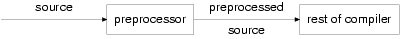
\includegraphics[type=pdf,read=.pdf,ext=.pdf,scale=0.8]
     {figure/7.1_preProc}
     \caption*{Diagram showing source code
       passing through a preprocessor to become 'preprocessed source',
       which is then fed into the rest of the compiler.}
     \caption{\label{fig:preProc}The preprocessor}
   \end{figure*}



  It's important to remember that the preprocessor is not working to the
   same rules as the rest of C. It works on a line-by-line basis, so the end
   of a line means something special to it. The rest of C thinks that
   end-of-line is little different from a space or tab character.


  The preprocessor doesn't know about the scope rules of C. Preprocessor
   directives like \texttt{\#define} take effect as soon as they are seen
   and remain in effect until the end of the file that contains them; the
   program's block structure is irrelevant. This is one of the reasons why
   it's a good idea to make sparing use of these directives. The less you
   have in your program that doesn't obey the `normal' scope rules,
   the less likely you are to make mistakes. This is mainly what gives rise
   to our comments about the poor level of integration between the
   preprocessor and the rest of C.


  The Standard gives some complicated rules for the syntax of the
   preprocessor, especially with respect to \textbf{tokens}. To understand
   the operation of the preprocessor you need to know a little about them.
   The text that is being processed is not considered to be a uniform stream
   of characters, but is separated into tokens then processed piecemeal.


  For a full definition of the process, it is best to refer to the
   Standard, but an informal description follows. Each of the terms used to
   head the list below is used later in descriptions of the rules.


  \begin{enumerate}
   \item \begin{center}\textit{header-name}\end{center}

    \begin{itemize}
     \item `\texttt{<}' \begin{center}\textit{almost any character}\end{center}

      `\texttt{>}'
    \end{itemize}
   
   \item \begin{center}\textit{preprocessing-token}\end{center}

    \begin{itemize}
     \item a \begin{center}\textit{header-name}\end{center}

 as above but only when the subject of
      \texttt{\#include},
     \item or an \begin{center}\textit{identifier}\end{center}

 which is any C identifier or
      keyword,
     \item or a \begin{center}\textit{constant}\end{center}

 which is any integral or floating
      constant,
     \item or a \begin{center}\textit{string-literal}\end{center}

 which is a normal C string,
     \item or an \begin{center}\textit{operator}\end{center}

 which is one of the C operators,
     \item or one of \begin{center}\textit{[ ] ( ) \{ \} * , : = ; ... \#}\end{center}

 (punctuators)
     \item or any non-white-space character not covered by the list above.
    \end{itemize}
   
  \end{enumerate}

  The `\begin{center}\textit{almost any character}\end{center}

' above means any character
   except `\texttt{>}' or newline.


 
   \section{Directives}
        

  

  Directives are always introduced by a line that starts with
   a \texttt{\#} character, optionally preceded by white space characters
   (although it isn't common practice to indent the \texttt{\#}).
   Table~\ref{tab:prepDir} below is a list of the directives defined in the
   Standard.


   \begin{table}[htb]
     \centering
     \begin{tabular}{ll}
       \toprule
       Directive          & Meaning   \\
       \midrule
       \texttt{\#include} & include a source file   \\
       \texttt{\#define}  & define a macro   \\
       \texttt{\#undef}   & undefine a macro   \\
       \texttt{\#if}      & conditional compilation   \\
       \texttt{\#ifdef}   & conditional compilation   \\
       \texttt{\#ifndef}  & conditional compilation   \\
       \texttt{\#elif}    & conditional compilation   \\
       \texttt{\#else}    & conditional compilation   \\
       \texttt{\#endif}   & conditional compilation   \\
       \texttt{\#line}    & control error reporting   \\
       \texttt{\#error}   & force an error message   \\
       \texttt{\#pragma}  & used for implementation-dependent control   \\
       \texttt{\#}        & null directive; no effect   \\
       \bottomrule
     \end{tabular}
     \caption{\label{tab:prepDir}Preprocessor directives}
   \end{table}


  The meanings and use of these features are described in the following
   sections. Make a note that the \texttt{\#} and the following keyword,
   if any, are individual items. They may be separated by white space.


  \subsection{The null directive}
   

   This is simple: a plain \texttt{\#} on a line by itself does
    nothing!


  

  \subsection{\# define}
   

   There are two ways of defining \textbf{macros}, one of which looks
    like a function and one which does not. Here is an example of each:


   \begin{Verbatim}
#define FMAC(a,b) a here, then b

#define NONFMAC some text here
\end{Verbatim}

   Both definitions define a macro and some \textbf{replacement text},
    which will be used to replace later occurrences of the macro name in the
    rest of the program. After those definitions, they can be used as
    follows, with the effect of the macro replacement shown in comments:


   \begin{Verbatim}
NONFMAC
/* some text here */

FMAC(first text, some more)
/* first text here, then some more */
\end{Verbatim}

   For the non-function macro, its name is simply replaced by its
    replacement text. The function macro is also replaced by its replacement
    text; wherever the replacement text contains an identifier which is the
    name of one of the macro's `formal parameters', the actual text
    given as the argument is used in place of the identifier in the
    replacement text. The scope of the names of the formal parameters is
    limited to the body of the \texttt{\#define} directive.


   For both forms of macro, leading or trailing white space around the
    replacement text is discarded.


   A curious ambiguity arises with macros: how do you define
    a non-function macro whose replacement text happens to start with the
    opening parenthesis character (? The answer is simple. If the definition
    of the macro has a space in front of the (, then it isn't the definition
    of a function macro, but a simple replacement macro instead. When you
    \textit{use} function-like macros, there's no equivalent
    restriction.


   The Standard allows either type of macro to be redefined at any time,
    using another \texttt{\# define}, provided that there isn't any
    attempt to change the type of the macro and that the tokens making up
    both the original definition and the redefinition are identical in
    number, ordering, spelling and use of white space. In this context all
    white space is considered equal, so this would be correct:


   \begin{Verbatim}
# define XXX abc/*comment*/def hij
# define XXX abc def hij
\end{Verbatim}

   because comment is a form of white space. The token sequence for both
    cases (\begin{center}\textit{w-s}\end{center}

 stands for a white-space token) is:


   \begin{Verbatim}
# w-s define w-s XXX w-s abc w-s def w-s hij w-s
\end{Verbatim}

   \subsubsection{Macro substitution}
    

    Where will occurrences of the macro name cause the replacement text
     to be substituted in its place? Practically anywhere in a program that
     the identifier is recognized as a separate token, except as the
     identifier following the \texttt{\#} of a preprocessor directive.
     You can't do this:


    \begin{Verbatim}
#define define XXX

#define YYY ZZZ
\end{Verbatim}

    and expect the second \texttt{\#define} to be replaced by
     \texttt{\#XXX}, causing an error.


    When the identifier associated with a non-function macro is seen, it
     is replaced by the macro replacement tokens, then \textbf{rescanned}
     (see later) for further replacements to make.


    Function macros can be used like real functions; white space around
     the macro name, the argument list and so on, may include the newline
     character:


    \begin{Verbatim}
#define FMAC(a, b) printf("%s %s\n", a, b)

FMAC ("hello",
      "sailor"
      );
/* results in */
printf("%s %s\n", "hello", "sailor")
\end{Verbatim}

    The `arguments' of a function macro can be almost any arbitrary
     token sequence. Commas are used to separate the arguments from each
     other but can be hidden by enclosing them within parentheses,
     \texttt{(} and \texttt{)}. Matched pairs of \texttt{(} and
     \texttt{)} inside the argument list balance each other out, so
     a \texttt{)} only ends the invocation of the macro if the
     corresponding ( is the one that started the macro invocation.


    \begin{Verbatim}
#define CALL(a, b) a b

CALL(printf, ("%d %d %s\n",1, 24, "urgh"));
/* results in */
printf ("%d %d %s\n",1, 24, "urgh");
\end{Verbatim}

    Note very carefully that the parentheses around the second argument
     to CALL were preserved in the replacement: they were not stripped from
     the text.


    If you want to use macros like \texttt{printt}, taking a variable
     number of arguments, the Standard is no help to you. They are not
     supported.


    If any argument contains no preprocessor tokens then the behaviour is
     undefined. The same is true if the sequence of preprocessor tokens that
     forms the argument would otherwise have been another preprocessor
     directive:


    \begin{Verbatim}
#define CALL(a, b) a b

/* undefined behaviour in each case.... */
CALL(,hello)
CALL(xyz,
#define abc def)
\end{Verbatim}

    In our opinion, the second of the erroneous uses of \texttt{CALL}
     \textit{should} result in defined behaviour--anyone capable of
     writing that would clearly benefit from the attentions of a champion
     weightlifter wielding a heavy leather bullwhip.


    When a function macro is being processed, the steps are as
     follows:


    \begin{enumerate}
     \item All of its arguments are identified.

     \item Except in the cases listed in item 3 below, if any of the tokens in
      an argument are themselves candidates for macro replacement, the
      replacement is done until no further replacement is possible. If
      this introduces commas into the argument list, there is no danger
      of the macro suddenly seeming to have a different number of
      arguments; the arguments are \textit{only} determined in the step
      above.

     \item In the macro replacement text, identifiers naming one of the macro
      formal arguments are replaced by the (by now expanded) token
      sequence supplied as the actual argument. The replacement is
      suppressed only if the identifier is preceded by one
      of \texttt{\#} or \texttt{\#\#}, or followed
      by \texttt{\#\#}.
    \end{enumerate}

   

   \subsubsection{Stringizing}
    

    There is special treatment for places in the macro replacement text
     where one of the macro formal parameters is found preceded by
     \texttt{\#}. The token list for the actual argument has any leading
     or trailing white space discarded, then the \texttt{\#} and the
     token list are turned into a single string literal. Spaces between the
     tokens are treated as space characters in the string. To prevent
     `unexpected' results, any \texttt{"}
     or \texttt{$\backslash$} characters within the new string literal are
     preceded by \texttt{$\backslash$}.


    This example demonstrates the feature:


    \begin{Verbatim}
#define MESSAGE(x) printf("Message: %s\n", #x)

MESSAGE (Text with "quotes");
/*
* Result is
* printf("Message: %s\n", "Text with \"quotes\"");
*/
\end{Verbatim}

   

   \subsubsection{Token pasting}
    

    A \texttt{\#\#} operator may occur anywhere in the replacement text
     for a macro except at the beginning or end. If a parameter name of
     a function macro occurs in the replacement text preceded or followed by
     one of these operators, the actual token sequence for the corresponding
     macro argument is used to replace it. Then, for both function and
     non-function macros, the tokens surrounding the \texttt{\#\#}
     operator are joined together. If they don't form a valid token, the
     behaviour is undefined. Then rescanning occurs.


    As an example of token pasting, here is a multi-stage operation,
     involving rescanning (which is described next).


    \begin{Verbatim}
#define REPLACE some replacement text
#define JOIN(a, b) a ## b

JOIN(REP, LACE)
becomes, after token pasting,
REPLACE
becomes, after rescanning
some replacement text
\end{Verbatim}

   

   \subsubsection{Rescanning}
    

    Once the processing described above has occurred, the replacement
     text plus the following tokens of the source file is rescanned, looking
     for more macro names to replace. The one exception is that, within
     a macro's replacement text, the name of the macro itself is not
     expanded. Because macro replacement can be nested, it is possible for
     several macros to be in the process of being replaced at any one point:
     none of their names is a candidate for further replacement in the
     `inner' levels of this process. This allows redefinition of
     existing functions as macros:


    \begin{Verbatim}
#define exit(x) exit((x)+1)
\end{Verbatim}

    These macro names which were not replaced now become tokens which are
     immune from future replacement, even if later processing might have
     meant that they had become available for replacement. This prevents the
     danger of infinite recursion occurring in the preprocessor. The
     suppression of replacement is only if the macro name results directly
     from \textit{replacement} text, not the other source text of the
     program. Here is what we mean:


    \begin{Verbatim}
#define m(x) m((x)+1)
/* so */
m(abc);
/* expands to */
m((abc)+1);
/*
* even though the m((abc)+1) above looks like a macro,
* the rules say it is not to be re-replaced
*/

m(m(abc));
/*
* the outer m( starts a macro invocation,
* but the inner one is replaced first (as above)
* with m((abc)+1), which becomes the argument to the outer call,
* giving us effectively
*/
m(m((abc+1));
/*
* which expands to
*/
m((m((abc+1))+1);
\end{Verbatim}

    If that doesn't make your brain hurt, then go and read what the
     Standard says about it, which will.


   

   \subsubsection{Notes}
    

    There is a subtle problem when using arguments to function
     macros.


    \begin{Verbatim}
/* warning - subtle problem in this example */
#define SQR(x)  ( x * x )
/*
* Wherever the formal parameters occur in
* the replacement text, they are replaced
* by the actual parameters to the macro.
*/
printf("sqr of %d is %d\n", 2, SQR(2));
\end{Verbatim}

    The formal parameter of \texttt{SQR} is \texttt{x}; the
     actual argument is \texttt{2}. The replacement text results in


    \begin{Verbatim}
printf("sqr of %d is %d\n", 2, ( 2 * 2 ));
\end{Verbatim}

    The use of the parentheses should be noticed. The following example
     is likely to give trouble:


    \begin{Verbatim}
/* bad example */
#define DOUBLE(y) y+y

printf("twice %d is %d\n", 2, DOUBLE(2));
printf("six times %d is %d\n", 2, 3*DOUBLE(2));
\end{Verbatim}

    The problem is that the last expression in the second printf is
     replaced by


    \begin{Verbatim}
3*2+2
\end{Verbatim}

    which results in \texttt{8}, not \texttt{12}! The rule is
     that when using macros to build expressions, careful parenthesizing is
     necessary. Here's another example:


    \begin{Verbatim}
SQR(3+4)

/* expands to */

( 3+4 * 3+4 )
/* oh dear, still wrong! */
\end{Verbatim}

    so, when formal parameters occur in the replacement text, you should
     look carefully at them too. Correct versions of \texttt{SQR} and
     \double{} are these:


    \begin{Verbatim}
#define SQR(x) ((x)*(x))
#define DOUBLE(x) ((x)+(x))
\end{Verbatim}

    Macros have a last little trick to surprise you with, as this
     shows.


    \VerbatimInput{example/example7-1.c}\begin{center}\textit{Example 7.1}\end{center}


    Why is this going to cause problems? Because the replacement text of
     the macro refers to \texttt{*ip++} twice, so \texttt{ip} gets
     incremented twice. Macros should never be used with expressions that
     involve side effects, unless you check very carefully that they are
     safe.


    Despite these warnings, they provide a very useful feature, and one
     which will be used a lot from now on.


   

  

  \subsection{\# undef}
   

   The name of any \texttt{\#define}d identifier can be forcibly
    forgotten by saying


   \begin{Verbatim}
#undef  NAME
\end{Verbatim}

   It isn't an error to \texttt{\#undef} a name which isn't currently
    defined.


   This occasionally comes in handy. Chapter~\ref{chap:libs} points out
    that some library functions may actually be macros, not functions, but
    by undefing their names you are guaranteed access to a real
    function.


  

  \subsection{\# include}
   

   This comes in two flavours:


   \begin{Verbatim}
#include <filename>
#include "filename"
\end{Verbatim}

   both of which cause a new file to be read at the point where they
    occur. It's as if the single line containing the directive is replaced
    by the contents of the specified file. If that file contains erroneous
    statements, you can reasonably expect that the errors will be reported
    with a correct file name and line number. It's the compiler writer's job
    to get that right. The Standard specifies that at least eight nested
    levels of \texttt{\# include} must be supported.


   The effect of using brackets \texttt{<>} or quotes
    \texttt{" "} around the filename is to change the places
    searched to find the specified file. The brackets cause a search of
    a number of implementation defined places, the quotes cause a search of
    somewhere associated with the original source file. Your implementation
    notes must tell you the specific details of what is meant by
    `place'. If the form using quotes can't find the file, it tries
    again as if you had used brackets.


   In general, brackets are used when you specify standard library header
    files, quotes are used for private header files--often specific to
    one program only.


   Although the Standard doesn't define what constitutes a valid file
    name, it does specify that there must be an implementation-defined
    unique way of translating file names of the form \texttt{xxx.x}
    (where \texttt{x} represents a `letter'), into source file
    names.  Distinctions of upper and lower case may be ignored and the
    implementation may choose only to use six significant characters before
    the `\texttt{.}' character.


   You can also write this:


   \begin{Verbatim}
# define NAME <stdio.h>
# include NAME
\end{Verbatim}

   to get the same effect as


   \begin{Verbatim}
# include <stdio.h>
\end{Verbatim}

   but it's a rather roundabout way of doing it, and unfortunately it's
    subject to implementation defined rules about how the text
    between \texttt{<} and \texttt{>} is
    treated.


   It's simpler if the replacement text for \texttt{NAME} comes out
    to be a string, for example


   \begin{Verbatim}
#define NAME "stdio.h"

#include NAME
\end{Verbatim}

   There is no problem with implementation defined behaviour here, but
    the paths searched are different, as explained above.


   For the first case, what happens is that the token sequence which
    replaces NAME is (by the rules already given)


   \begin{Verbatim}
<
stdio
.
h
>
\end{Verbatim}

   and for the second case


   \begin{Verbatim}
"stdio.h"
\end{Verbatim}

   The second case is easy, since it's just a \begin{center}\textit{string-literal}\end{center}

    which is a legal token for a \texttt{\# include} directive. It is
    implementation defined how the first case is treated, and whether or not
    the sequence of tokens forms a legal \begin{center}\textit{header-name}\end{center}

.


   Finally, the last character of a file which is being
    \texttt{include}d must be a plain newline. Failure to include a file
    successfully is treated as an error.


  

  \subsection{Predefined names}
   

   The following names are predefined within the preprocessor:


   \begin{description}
    \item[\texttt{\_\_LINE\_\_}] The current source file line number, a decimal integer constant.

    \item[\texttt{\_\_FILE\_\_}] The `name' of the current source code file, a string
     literal.

    \item[\texttt{\_\_DATE\_\_}] 
     The current date, a string literal. The form is

     \begin{Verbatim}
Apr 21 1990
\end{Verbatim}

     where the month name is as defined in the library function
      \texttt{asctime} and the first digit of the date is a space if
      the date is less than 10.

    

    \item[\texttt{\_\_TIME\_\_}] The time of the translation; again a string literal in the form
     produced by asctime, which has the form \texttt{"hh:mm:ss"}.

    \item[\texttt{\_\_STDC\_\_}] 
     The integer constant 1. This is used to test if the compiler is
      Standard-conforming, the intention being that it will have different
      values for different releases of the Standard.

     A common way of using these predefined names is the following:


     \VerbatimInput{example/example7-2.c}\begin{center}\textit{Example 7.2}\end{center}


    
   \end{description}

   If the argument to \texttt{TEST} gives a false result, the message
    is printed, including the filename and line number in the message.


   There's only one minor caveat: the use of the \kif{}
    statement can cause confusion in a case like this:


   \begin{Verbatim}
if(expression)
      TEST(expr2);
else
      statement_n;
\end{Verbatim}

   The else will get associated with the hidden if generated by expanding
    the \texttt{TEST} macro. This is most unlikely to happen in
    practice, but will be a thorough pain to track down if it ever does
    sneak up on you. It's good style to make the bodies of every control of
    flow statement compound anyway; then the problem goes away.


   None of the names \texttt{\_\_LINE\_\_}, \texttt{\_\_FILE\_\_},
    \texttt{\_\_DATE\_\_}, \texttt{\_\_TIME\_\_}, \texttt{\_\_STDC\_\_} or
    defined may be used in \texttt{\#define} or \texttt{\#undef}
    directives.


   The Standard specifies that any other reserved names will either start
    with an underscore followed by an upper case letter or another
    underscore, so you know that you are free to use any other names for
    your own purposes (but watch out for additional names reserved in
    Library header files that you may have included).


  

  \subsection{\#line}
   

   This is used to set the value of the built in names
    \texttt{\_\_LINE\_\_} and \texttt{\_\_FILE\_\_}. Why do this? Because
    a lot of tools nowadays actually generate C as their output. This
    directive allows them to control the current line number. It is of very
    limited interest to the `ordinary' C programmer.


   Its form is


   \begin{Verbatim}
# line number optional-string-literal newline
\end{Verbatim}

   The number sets the value of \texttt{\_\_LINE\_\_}, the string
    literal, if present, sets the value of \texttt{\_\_FILE\_\_}.


   In fact, the sequence of tokens following \texttt{\#line} will be
    macro expanded. After expansion, they are expected to provide a valid
    directive of the right form.


  

  \subsection{Conditional compilation}
   

   A number of the directives control conditional compilation, which
    allows certain portions of a program to be selectively compiled or
    ignored depending upon specified conditions. The directives concerned
    are: \texttt{\#if}, \texttt{\#ifdef}, \texttt{\#ifndef},
    \texttt{\#elif}, \texttt{\#else}, \texttt{\#endif} together
    with the preprocessor unary operator defined.


   The way that they are used is like this:


   \begin{Verbatim}
#ifdef  NAME
/* compile these lines if NAME is defined */
#endif
#ifndef NAME
/* compile these lines if NAME is not defined */
#else
/* compile these lines if NAME is defined */
#endif
\end{Verbatim}

   So, \texttt{\#ifdef} and \texttt{\#endif} can be used to test
    the definition or otherwise of a given macro name. Of course the
    \texttt{\#else} can be used with \texttt{\#ifdef} (and
    \texttt{\#if} or \texttt{\#elif}) too. There is no ambiguity about
    what a given \texttt{\#else} binds to, because the use of
    \texttt{\#endif} to delimit the scope of these directives eliminates
    any possible ambiguity. The Standard specifies that at least eight
    levels of nesting of conditional directives must be supported, but in
    practice there is not likely to be any real limit.


   These directives are most commonly used to select small fragments of
    C that are machine specific (when it is not possible to make the whole
    program completely machine independent), or sometimes to select
    different algorithms depending on the need to make trade-offs.


   The \texttt{\#if} and \texttt{\#elif} constructs take a single
    integral constant expression as their arguments. Preprocessor integral
    constant expressions are the same as other integral constant expressions
    except that they must not contain cast operators. The token sequence
    that makes up the constant expression undergoes macro replacement,
    except that names prefixed by defined are not expanded. In this context,
    the expression \texttt{defined NAME} or \texttt{defined ( NAME
    )} evaluates to \texttt{1} if \texttt{NAME} is currently
    defined, \texttt{0} if it is not. Any other identifiers in the
    expression \textit{including those that are C keywords} are replaced
    with the value \texttt{0}. Then the expression is evaluated. The
    replacement even of keywords means that \sizeof{} can't be
    used in these expressions to get the result that you would normally
    expect.


   As with the other conditional statements in C, a resulting value of
    zero is used to represent `false', anything else is
    `true'.


   The preprocessor always must use arithmetic with at least the ranges
    defined in the \texttt{<limits.h>} file and treats int
    expressions as long int and unsigned int as unsigned long int. Character
    constants do not necessarily have the same values as they do at
    execution time, so for highly portable programs, it's best to avoid
    using them in preprocessor expressions. Overall, the rules mean that it
    is possible to get arithmetic results from the preprocessor which are
    different from the results at run time; although presumably only if the
    translation and execution are done on different machines. Here's an
    example.


   \VerbatimInput{example/example7-3.c}\begin{center}\textit{Example 7.3}\end{center}


   It is conceivable that the preprocessor might perform arithmetic with
    a greater range than that used in the target environment. In that case,
    the preprocessor expression \texttt{ULONG\_MAX+1} might not
    `overflow' to give the result of \texttt{0}, whereas in the
    execution environment, it \textit{must}.


   The following skeleton example illustrates the use of such constants
    and also the `conditional else', \texttt{\#elif}.


   \begin{Verbatim}
#define NAME    100

#if     ((NAME > 50) && (defined __STDC__))
/* do something */
#elif   NAME > 25
/* do something else*/
#elif   NAME > 10
/* do something else */
#else
/* last possibility */
#endif
\end{Verbatim}

   A word of warning. These conditional compilation directives do not
    obey the same scope rules as the rest of C. They should be used
    sparingly, unless your program is rapidly to become unreadable. It is
    impossible to read C when it is laced with these things every few lines.
    The urge to maim the author of a piece of code becomes very strong when
    you suddenly come across


   \begin{Verbatim}
#else
      }
#endif
\end{Verbatim}

   with no \texttt{\#if} or whatever immediately visible above. They
    should be treated like chilli sauce; essential at times, but more than
    a tiny sprinkle is too much.


  

  \subsection{\#pragma}
   

   This was the Standard Committee's way of `opening the back
    door'. It allows implementation-defined things to take place. If the
    implementation was not expecting what you wrote (i.e. doesn't recognize
    it), it is ignored. Here is a possible example:


   \begin{Verbatim}
#pragma byte_align
\end{Verbatim}

   which could be used to tell the implementation that all structure
    members should be aligned on byte addresses - some processor
    architectures are able to cope with word-sized structure members aligned
    on byte addresses, but with a penalty in access speed being
    incurred.


   It could, of course, mean anything else that the implementation
    chooses it to mean.


   If your implementation doesn't have any special meaning for this, then
    it will have no effect. It will \textit{not} count as an error.


   It will be interesting to see the sort of things that this gets used
    for.


  

  \subsection{\#error}
   

   This directive is followed by one or more tokens at the end of the
    line. A diagnostic message is produced by the compiler, which includes
    those tokens, but no further detail is given in the Standard. It might
    be used like this to abort a compilation on unsuitable hardware:


   \begin{Verbatim}
#include <limits.h>
#if CHAR_MIN > -128
#error character range smaller than required
#endif
\end{Verbatim}

   which would be expected to produce some sort of meaningful compilation
    error and message.


  

 
        \section{Summary}
        


  To be honest, although many of the facilities provided by the
   preprocessor undoubtedly provide extra power and flexibility, it
   really is rather overcomplicated.


  There are only a very few aspects that are really important.


  The ability to define macros and function macros is very important,
   being widely used in almost every C program except the most trivial.


  The conditional compilation has two important uses; one is the
   ability to compile with or without debugging statements included in
   a program, the other is to be able to select machine or application
   dependent statements.


  Obviously, file inclusion is fundamentally important.


  Having said the above, most of the rest of the features described in
   this chapter can be forgotten with very little loss of functionality.
   Perhaps each programming team should have just one preprocessor
   specialist who has the job of designing project-dependent macros using
   the arcane features such as stringizing and token pasting. Most users
   of C would benefit much more by putting that learning effort into other
   parts of the language, or, when they fully understand C, techniques of
   software quality control. The world would be a better place.


 
        \section{Exercises}
        


  These exercises are intended to test only a basic understanding of
   the preprocessor, suitable for a beginner. Many users will never
   need a more detailed understanding.


  \textbf{Exercise 7.1.} How would you arrange that the identifier
   \texttt{MAXLEN} is replaced by the value \texttt{100} throughout
   a program?


  \textbf{Exercise 7.2.} What is likely to cause problems in a definition of
   the form \texttt{\#define VALUE 100+MAXLEN}?


  \textbf{Exercise 7.3.} Write a macro called \texttt{REM} which takes
   two integer arguments and `returns' the remainder when the first
   is divided by the second.


  \textbf{Exercise 7.4.} Repeat the last example, but use casts so that any
   arithmetic type of argument may be used, assuming that there are no
   overflow problems.


  \textbf{Exercise 7.5.} What do the \texttt{<>} brackets around
   a filename in a \texttt{\#include} directive signify?


  \textbf{Exercise 7.6.} What would \texttt{""} mean in place of
   the \texttt{<>}?


  \textbf{Exercise 7.7.} How would you use the preprocessor to select
   implementation-specific fragments of a program?


  \textbf{Exercise 7.8.} What sort of arithmetic does the preprocessor
   use?


 \chapter{Specialized Areas of C}\label{chap:special}


        \section{Government Health Warning}
        

  

  The previous chapters have introduced the fundamentals of the language
   and have covered nearly all of the language that the Standard defines.
   There are a number of murky and convoluted backwaters left unexplored on
   grounds of sympathy and compassion for the sufferer, and some without any
   better home. This chapter gathers them together--it's the toxic waste
   dump for the nasty bits of C.


  Pull on your rubber gloves, read the following sections and make notes
   where you think the material is important to you; re-read them from time
   to time as well. What seemed uninteresting and painful the first time
   round may change as your experience grows, or your natural immunity
   improves.


  What we cover here is \textit{not} an exhumation of all the pathogenic
   elements--we leave that for another book--but it does serve to
   round up most of the commonly encountered difficult or extraordinary
   material.


 
        \section{Declarations, Definitions and Accessibility}
        

  

  Chapter~\ref{chap:funcs} introduced the concepts of \textbf{scope} and
   \textbf{linkage}, showing how they can be combined to control the
   accessibility of things throughout a program. We deliberately gave
   a vague description of exactly what constitutes a \textbf{definition}
   on the grounds that it would give you more pain than gain at that stage.
   Eventually it has to be spelled out in detail, which we do in this
   chapter. Just to make things interesting, we need to throw in
   \textbf{storage class} too.


  You'll probably find the interactions between these various elements to
   be both complex and confusing: that's because they are! We try to
   eliminate some of the confusion and give some useful rules of thumb in
   Section 8.2.6 (reference does not exist) below--but to understand them, you still
   need to read the stuff in between at least once.


  For a full understanding, you need a good grasp of three distinct but
   related concepts. The Standard calls them:


  \begin{itemize}
   \item duration
   \item scope
   \item linkage
  \end{itemize}

  and describes what they mean in a fairly readable way (for a standard).
   Scope and linkage have already been described in Chapter~\ref{chap:funcs},
   although we do present a review of them below.


  \subsection{Storage class specifiers}
   

   There are five keywords under the category of \textbf{storage class
    specifiers}, although one of them, \typedef, is there
    more out of convenience than utility; it has its own section later since
    it doesn't really belong here. The ones remaining are \auto,
    \extern, \register, and \static.


   Storage class specifiers help you to specify the type of storage used
    for data objects. Only one storage class specifier is permitted in
    a declaration--this makes sense, as there is only one way of storing
    things--and if you omit the storage class specifier in
    a declaration, a default is chosen. The default depends on whether the
    declaration is made outside a function (external declarations) or inside
    a function (internal declarations). For external declarations the
    default storage class specifier will be \extern{} and for
    \texttt{internal} declarations it will be \auto. The
    only exception to this rule is the declaration of functions, whose
    \textit{default} storage class specifier is always
    \extern.


   The positioning of a declaration, the storage class specifiers used
    (or their defaults) and, in some cases, preceding declarations of the
    same name, can all affect the linkage of a name, although fortunately
    not its scope or duration. We will investigate the easier items
    first.


   \subsubsection{Duration}
    

    The \textbf{duration} of an object describes whether its storage is
     allocated once only, at program start-up, or is more transient in its
     nature, being allocated and freed as necessary.


    There are only two types of duration of objects: \textbf{static
     duration} and \textbf{automatic duration}. Static duration means
     that the object has its storage allocated permanently, automatic means
     that the storage is allocated and freed as necessary. It's easy to tell
     which is which: you only get automatic duration if


    \begin{itemize}
     \item the declaration is inside a function
     \item \textit{and} the declaration does not contain the
      \static{} or \extern{} keywords
     \item \textit{and} the declaration is not the declaration of a function
    \end{itemize}

    (if you work through the rules, you'll find that the formal
     parameters of a function always meet all three requirements--they
     are always `automatic').


    Although the presence of \static{} in a declaration
     unambiguously ensures that it has static duration, it's interesting to
     see that it is by no means the only way. This is a notorious source of
     confusion, but we just have to accept it.


    Data objects declared inside functions are given the default storage
     class specifier of \auto{} unless some other storage class
     specifier is used. In the vast majority of cases, you don't want these
     objects to be accessible from outside the function, so you want them to
     have \textit{no linkage}. Either the default, \auto, or the
     explicit \register{} storage class specifier results in an
     object with no linkage and \textbf{automatic duration}. Neither
     \auto{} nor \register{} can be applied to
     a declaration that occurs outside a function.


    The \register{} storage class is quite interesting,
     although it is tending to fall into disuse nowadays. It suggests to the
     compiler that it would be a good idea to store the object in one or
     more hardware registers in the interests of speed. The compiler does
     not have to take any notice of this, but to make things easy for it,
     \register{} variables do not have an address (the
     \texttt{\&} address-of operator is forbidden) because some
     computers don't support the idea of addressable registers. Declaring
     too many \register{} objects may slow the program down,
     rather than speed it up, because the compiler may either have to save
     more registers on entrance to a function, often a slow process, or
     there won't be enough registers remaining to be used for intermediate
     calculations. Determining when to use registers will be
     a machine-specific choice and should only be taken when detailed
     measurements show that a particular function needs to be speeded up.
     Then you will have to experiment. In our opinion, you should never
     declare register variables during program development. Get the program
     working first, then measure it, then, maybe, judicious use of registers
     will give a useful increase in performance. But that work will have to
     be repeated for every type of processor you move the program to; even
     within one family of processors the characteristics are often
     different.


    A final note on \register{} variables: this is the only
     storage class specifier that may be used in a function prototype or
     function definition. In a function prototype, the storage class
     specifier is simply ignored, in a function definition it is a hint that
     the actual parameter should be stored in a register if possible. This
     example shows how it might be used:


     \VerbatimInput{example/example8-1.c}
     \begin{center}\textit{Example 8.1}\end{center}


    So, the duration of an object depends on the storage class specifier
     used, whether it's a data object or function, and the position (block
     or file scope) of the declaration concerned. The linkage is also
     dependent on the storage class specifier, what kind of object it is and
     the scope of the declaration.
     Table~\ref{tab:extDecl} and Table~\ref{tab:interDecl}
     show the resulting storage duration and apparent linkage
     for the various combinations of storage class specifiers and location
     of the declaration. The actual linkage of objects with static duration
     is a bit more complicated, so use these tables only as a guide to the
     simple cases and take a look at what we say later about
     definitions.

     \begin{table}[htb]
       \centering
       \begin{tabular}{p{.17\textwidth}p{.16\textwidth}ll}
         \toprule
         Storage Class Specifier & Function or Data Object & Linkage & Duration \\
         \midrule
         \static{} & either      & internal          & static     \\
         \extern{} & either      & probably external & static     \\
         none            & function    & probably external & static     \\
         none            & data object & external          & static     \\
         \bottomrule
       \end{tabular}
       \caption{\label{tab:extDecl}External declarations (outside a function}
     \end{table}


    The table above omits the \register{} and \auto{}
     storage class specifiers because they are not permitted in file-scope
     (external) declarations.

     \begin{table}[htb]
       \centering
       \begin{tabular}{p{.17\textwidth}p{.16\textwidth}ll}
         \toprule
         Storage Class Specifier & Function or Data Object & Linkage & Duration \\
         \midrule
         \register{} & data object only & none              & automatic \\
         \auto       & data object only & none              & automatic \\
         \static{}   & data object only & none              & static    \\
         \extern{}   & either           & probably external & static    \\
         none        & data object      & none              & automatic \\
         none        & function         & probably external & static    \\
         \bottomrule
       \end{tabular}
       \caption{\label{tab:interDecl}Internal declarations}
     \end{table}


    Internal \static{} variables retain their values between
     calls of the function that contains them, which is useful in certain
     circumstances (see Chapter~\ref{chap:funcs}).


   

  

  \subsection{Scope}
   

   Now we must look again at the \textbf{scope} of the names of
    objects, which defines when and where a given name has a particular
    meaning. The different types of scope are the following:


   \begin{itemize}
    \item function scope
    \item file scope
    \item block scope
    \item function prototype scope
   \end{itemize}

   The easiest is \textbf{function scope}. This only applies to labels,
    whose names are visible throughout the function where they are declared,
    irrespective of the block structure. No two labels in the same function
    may have the same name, but because the name only has function scope,
    the same name can be used for labels in every function. Labels are
    \textit{not} objects--they have no storage associated with them and
    the concepts of linkage and duration have no meaning for them.


   Any name declared outside a function has \textbf{file scope}, which
    means that the name is usable at any point from the declaration on to
    the end of the source code file containing the declaration. Of course it
    is possible for these names to be temporarily hidden by declarations
    within compound statements. As we know, function definitions
    \textit{must} be outside other functions, so the name introduced by any
    function definition will always have file scope.


   A name declared inside a compound statement, or as a formal parameter
    to a function, has \textbf{block scope} and is usable up to the end of
    the associated \texttt{\}} which closes the compound statement. Any
    declaration of a name within a compound statement hides any outer
    declaration of the same name until the end of the compound
    statement.


   A special and rather trivial example of scope is \textbf{function
    prototype scope} where a declaration of a name extends only to the
    end of the function prototype. That means simply that this is wrong
    (same name used twice):


\begin{Verbatim}
void func(int i, int i);
\end{Verbatim}

   and this is all right:


\begin{Verbatim}
void func(int i, int j);
\end{Verbatim}

   The names declared inside the parentheses disappear outside them.


   The scope of a name is completely independent of any storage class
    specifier that may be used in its declaration.


  

  \subsection{Linkage}
   

   We will briefly review the subject of \textbf{linkage} here, too.
    \textbf{Linkage} is used to determine what makes the same name
    declared in different scopes refer to the same thing. An object only
    ever has one name, but in many cases we would like to be able to refer
    to the same object from different scopes. A typical example is the wish
    to be able to call \texttt{printf} from several different places in
    a program, even if those places are not all in the same source file.


   The Standard warns that declarations which refer to the same thing
    must all have compatible type, or the behaviour of the program will be
    undefined. A full description of compatible type is given later; for the
    moment you can take it to mean that, except for the use of the storage
    class specifier, the declarations must be identical. It's the
    responsibility of the programmer to get this right, though there will
    probably be tools available to help you check this out.


   The three different types of linkage are:


   \begin{itemize}
    \item external linkage
    \item internal linkage
    \item no linkage
   \end{itemize}

   In an entire program, built up perhaps from a number of source files
    and libraries, if a name has \textbf{external linkage}, then every
    instance of a that name refers to the same object throughout the
    program.


   For something which has \textbf{internal linkage}, it is only within
    a given source code file that instances of the same name will refer to
    the same thing.


   Finally, names with \textbf{no linkage} refer to separate
    things.


  

  \subsection{Linkage and definitions}
   

   Every data object or function that is actually used in a program
    (except as the operand of a \sizeof{} operator) \textit{must have
    one and only one} corresponding \textbf{definition}. This is
    actually very important, although we haven't really come across it yet
    because most of our examples have used only data objects with automatic
    duration, whose declarations are axiomatically definitions, or functions
    which we have defined by providing their bodies.


   This `exactly one' rule means that for objects with external
    linkage there must be exactly one definition in the whole program; for
    things with internal linkage (confined to one source code file) there
    must be exactly one definition in the file where it is declared; for
    things with no linkage, whose declaration is always a definition, there
    is exactly one definition as well.


   Now we try to draw everything together. The real questions are


   \begin{enumerate}
    \item How do I get the sort of linkage that I want?
    \item What actually constitutes a definition?
   \end{enumerate}

   We need to look into linkage first, then definitions.


   How do you get the appropriate linkage for a particular name? The
    rules are a little complicated.


   \begin{enumerate}
    \item A declaration outside a function (file scope) which contains the
     \static{} storage class specifier results in \textbf{internal linkage}
     for that name. (The Standard requires that function declarations which
     contain \static{} \textit{must} be at file scope, outside any
     block)

    \item If a declaration contains the \extern{} storage class
     specifier, or is the declaration of a function with no storage class
     specifier (or both), then:

     \begin{itemize}
      \item If there is already a visible declaration of that identifier
       with file scope, the resulting linkage is the same as that of
       the visible declaration;

      \item otherwise the result is \textbf{external linkage}.
     \end{itemize}
    

    \item If a file scope declaration is neither the declaration of a
     function nor contains an explicit storage class specifier, then the
     result is \textbf{external linkage}.

    \item Any other form of declaration results in \textbf{no linkage}.

    \item In any one source code file, if a given identifer has both internal
     and external linkage then the result is undefined.
   \end{enumerate}

   These rules were used to derive the `linkage' columns of
     Table~\ref{tab:extDecl} and Table~\ref{tab:interDecl}, without the full
    application of rule 2--hence the use of the `probably
    external' term. Rule 2 allows you to determine the precise linkage in
    those cases.


   What makes a declaration into a definition?


   \begin{itemize}
    \item Declarations that result in no linkage are also definitions.

    \item Declarations that include an initializer are always definitions;
     this includes the `initialization' of functions by providing their
     body. Declarations with block scope may only have initializers if
     they also have no linkage.

    \item Otherwise, the declaration of a name with file scope and with
     either no storage class specifier or with the \static{}
     storage class specifier is a \textbf{tentative definition}. If
     a source code file contains one or more tentative definitions for
     an object, then if that file contains no actual definitions, a
     default definition is provided for that object as if it had an
     initializer of \texttt{0}. (Structures and arrays have
     all their elements initialized to \texttt{0}). Functions
     do not have tentative definitions.
   \end{itemize}

   A consequence of the foregoing is that unless you also provide an
    initializer, declarations that explicitly include the extern storage
    class specifier do \textit{not} result in a definition.


  

  \subsection{Realistic use of linkage and definitions}
   

   The rules that determine the linkage and definition associated with
    declarations look quite complicated. The combinations used in practice
    are nothing like as bad; so let's investigate the usual cases.


   The three types of accessibility that you will want of data objects or
    functions are:


   \begin{itemize}
    \item throughout the entire program,

    \item restricted to one source file,

    \item restricted to one function (or perhaps a single compound
     statement).
   \end{itemize}

   For the three cases above, you will want external linkage, internal
    linkage, and no linkage respectively. The recommended practice for the
    first two cases is to declare all of the names in each of the relevant
    source files \textit{before} you define any functions. The recommended
    layout of a source file would be as shown in Figure~\ref{fig:srcFile}.


    \begin{figure*}\centering
      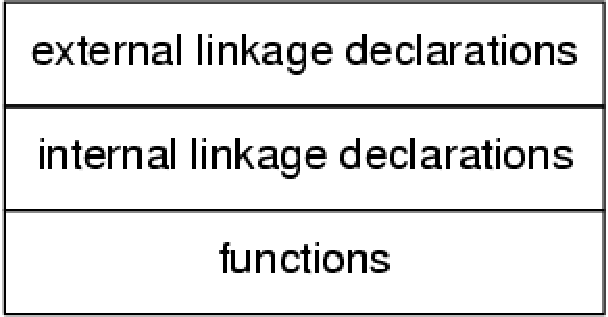
\includegraphics[type=pdf,read=.pdf,ext=.pdf,scale=1.0]
      {figure/8.1_srcFile}
      \caption*{Diagram showing the typical layout of a C source file,
        starting with external linkage declarations,
        which are followed by internal linkage declarations,
        and then functions at the end.}
      \caption{\label{fig:srcFile}Layout of a source file}
    \end{figure*}



   The external linkage declarations would be prefixed with extern, the
    internal linkage declarations with \static. Here's an
    example.


    \VerbatimInput{example/example8-2.c}
    \begin{center}\textit{Example 8.2}\end{center}


   We suggest that your re-read the preceding sections to see how the
    rules have been applied in Example 8.2.


  

 
        \section{Typedef}
        

  

  Although typedef is thought of as being a storage class, it isn't
   really. It allows you to introduce synonyms for types which could have
   been declared some other way. The new name becomes equivalent to the type
   that you wanted, as this example shows.


\begin{Verbatim}
typedef int aaa, bbb, ccc;
typedef int ar[15], arr[9][6];
typedef char c, *cp, carr[100];

/* now declare some objects */

/* all ints */
aaa     int1;
bbb     int2;
ccc     int3;

ar      yyy;    /* array of 15 ints */
arr     xxx;    /* 9*6 array of int */

c       ch;     /* a char */
cp      pnt;    /* pointer to char */
carr    chry;   /* array of 100 char */
\end{Verbatim}

  The general rule with the use of typedef is to write out a declaration
   as if you were declaring variables of the types that you want. Where
   a declaration would have introduced names with particular types,
   prefixing the whole thing with typedef means that, instead of getting
   variables declared, you declare new type names instead. Those new type
   names can then be used as the prefix to the declaration of variables of
   the new type.


  The use of \typedef{} isn't a particularly common sight in
   most programs; it's typically found only in header files and is rarely
   the province of day-to-day coding.


  It is sometimes found in applications requiring very high portability:
   there, new types will be defined for the basic variables of the program
   and appropriate \typedef{}s used to tailor the program to the
   target machine. This can lead to code which C programmers from other
   environments will find difficult to interpret if it's used to excess. The
   flavour of it is shown below:


\begin{Verbatim}
/* file 'mytype.h' */
typedef short   SMALLINT        /* range *******30000 */
typedef int     BIGINT          /* range ******* 2E9 */

/* program */
#include "mytype.h"

SMALLINT        i;
BIGINT          loop_count;
\end{Verbatim}

  On some machines, the range of an int would not be adequate for
   a \texttt{BIGINT} which would have to be re- \typedef{}'d
   to be \klong.


  To re-use a name already declared as a \typedef, its
   declaration must include at least one type specifier, which removes any
   ambiguity:


\begin{Verbatim}
typedef int new_thing;
func(new_thing x){
        float new_thing;
        new_thing = x;
}
\end{Verbatim}

  As a word of warning, \typedef{} can only be used to declare
   the type of return value from a function, not the overall type of the
   function. The overall type includes information about the function's
   parameters as well as the type of its return value.


\begin{Verbatim}
/*
 * Using typedef, declare 'func' to have type
 * 'function taking two int arguments, returning int'
 */
typedef int func(int, int);

/* ERROR */
func func_name{ /*....*/ }

/* Correct. Returns pointer to a type 'func' */
func *func_name(){ /*....*/ }

/*
 * Correct if functions could return functions,
 * but C can't.
 */
func func_name(){ /*....*/ }
\end{Verbatim}

  If a \typedef{} of a particular identifier is in scope, that
   identifer may not be used as the formal parameter of a function. This is
   because something like the following declaration causes a problem:


\begin{Verbatim}
typedef int i1_t, i2_t, i3_t, i4_t;

int f(i1_t, i2_t, i3_t, i4_t)/*THIS IS POINT 'X'*/
\end{Verbatim}

  A compiler reading the function declaration reaches point `X' and
   still doesn't know whether it is looking at a function declaration,
   essentially similar to


\begin{Verbatim}
int f(int, int, int, int) /* prototype */
\end{Verbatim}

  or


\begin{Verbatim}
int f(a, b, c, d) /* not a prototype */
\end{Verbatim}

  --the problem is only resolvable (in the worst case) by looking at
   what follows point `X'; if it is a semicolon, then that was
   a declaration, if it is a \texttt{\{} then that was a definition. The
   rule forbidding typedef names to be formal parameters means that
   a compiler can always tell whether it is processing a declaration or
   a definition by looking at the first identifier following the function
   name.


  The use of typedef is also valuable when you want to declare things
   whose declaration syntax is painfully impenetrable, like `array of ten
   pointers to array of five integers', which tends to cause panic even
   amongst the hardy. Hiding it in a typedef means you only have to read it
   once and can also help to break it up into manageable pieces:


\begin{Verbatim}
typedef int (*a10ptoa5i[10])[5];
/* or */
typedef int a5i[5];
typedef a5i *atenptoa5i[10];
\end{Verbatim}

  Try it out!


 
        \section{Const and volatile}
        

  

  These are new in Standard C, although the idea of \const{}
   has been borrowed from C++. Let us get one thing straight: the concepts
   of \const{} and \volatile{} are \textit{completely
   independent}. A common misconception is to imagine that somehow
   \const{} is the opposite of \volatile{} and vice
   versa. They are unrelated and you should remember the fact.


  Since \const{} declarations are the simpler, we'll look at
   them first, but only after we have seen where both of these type
   qualifiers may be used. The complete list of relevant keywords is


\begin{Verbatim}
char      long      float     volatile
short     signed    double    void
int       unsigned  const
\end{Verbatim}

  In that list, \const{} and \volatile{} are type
   qualifiers, the rest are \textbf{type specifiers}. Various combinations
   of type specifiers are permitted:


\begin{Verbatim}
char, signed char, unsigned char
int, signed int, unsigned int
short int, signed short int, unsigned short int
long int, signed long int, unsigned long int
float
double
long double
\end{Verbatim}

  A few points should be noted. All declarations to do with an
   \kint{} will be \signed{} anyway, so signed is
   redundant in that context. If \textit{any} other type specifier or
   qualifier is present, then the int part may be dropped, as that is the
   default.


  The keywords \const{} and \volatile{} can be
   applied to any declaration, including those of structures, unions,
   enumerated types or \typedef{} names. Applying them to
   a declaration is called \textbf{qualifying} the declaration--that's
   why const and volatile are called type qualifiers, rather than type
   specifiers. Here are a few representative examples:


\begin{Verbatim}
volatile i;
volatile int j;
const long q;
const volatile unsigned long int rt_clk;
struct {
  const long int li;
  signed char sc;
} volatile vs;
\end{Verbatim}

  Don't be put off; some of them are deliberately complicated: what they
   mean will be explained later. Remember that they could also be further
   complicated by introducing storage class specifications as well! In fact,
   the truly spectacular


\begin{Verbatim}
extern const volatile unsigned long int rt_clk;
\end{Verbatim}

  is a strong possibility in some real-time operating system kernels.


  \subsection{Const}
   

   Let's look at what is meant when \const{} is used. It's
    really quite simple: \const{} means that something is not
    modifiable, so a data object that is declared with \const{} as
    a part of its type specification must not be assigned to in any way
    during the run of a program. It is very likely that the definition of
    the object will contain an initializer (otherwise, since you can't
    assign to it, how would it ever get a value?), but this is not always
    the case. For example, if you were accessing a hardware port at a fixed
    memory address and promised only to read from it, then it would be
    declared to be \const{} but not initialized.


   Taking the address of a data object of a type which isn't
    \const{} and putting it into a pointer to the
    \const-qualified version of the same type is both safe and
    explicitly permitted; you will be able to use the pointer to inspect the
    object, but not modify it. Putting the address of a const type into
    a pointer to the unqualified type is much more dangerous and
    consequently prohibited (although you can get around this by using
    a cast). Here is an example:


    \VerbatimInput{example/example8-3.c}
    \begin{center}\textit{Example 8.3}\end{center}


   As the example shows, it is possible to take the address of a constant
    object, generate a pointer to a non-constant, then use the new pointer.
    This is an \textit{error} in your program and results in undefined
    behaviour.
    %% **** this is not what the program shows:
    %% as cpi is in fact a copy of ncpi which is copied back to ncpi,
    %% the ncpi is a pointer not to a constant.
    %% Thus the behavior is indeed defined. 


   The main intention of introducing const objects was to allow them to
    be put into read-only store, and to permit compilers to do extra
    consistency checking in a program. Unless you defeat the intent by doing
    naughty things with pointers, a compiler is able to check that
    \const{} objects are not modified explicitly by the user.


   An interesting extra feature pops up now. What does this mean?


\begin{Verbatim}
char c;
char *const cp = &c;
\end{Verbatim}

   It's simple really; \texttt{cp} is a pointer to
    a \kchar, which is exactly what it would be if the
    \const{} weren't there. The \const{} means that
    \texttt{cp} is not to be modified, although whatever it points to
    can be--the pointer is constant, not the thing that it points to.
    The other way round is


\begin{Verbatim}
const char *cp;
\end{Verbatim}

   which means that now cp is an ordinary, modifiable pointer, but the
    thing that it points to must not be modified. So, depending on what you
    choose to do, both the pointer and the thing it points to may be
    modifiable or not; just choose the appropriate declaration.


  

  \subsection{Volatile}
   

   After const, we treat \volatile. The reason for having
    this type qualifier is mainly to do with the problems that are
    encountered in real-time or embedded systems programming using C.
    Imagine that you are writing code that controls a hardware device by
    placing appropriate values in hardware registers at known absolute
    addresses.


   Let's imagine that the device has two registers, each 16 bits long, at
    ascending memory addresses; the first one is the control and status
    register (csr) and the second is a data port. The traditional way of
    accessing such a device is like this:


    \VerbatimInput{example/example8-4.c}
    \begin{center}\textit{Example 8.4}\end{center}


   The technique of using a structure declaration to describe the device
    register layout and names is very common practice. Notice that there
    aren't actually any objects of that type defined, so the declaration
    simply indicates the structure without using up any store.


   To access the device registers, an appropriately cast constant is used
    as if it were pointing to such a structure, but of course it points to
    memory addresses instead.


   However, a major problem with previous C compilers would be in the
    while loop which tests the status register and waits for the
    \texttt{ERROR} or \texttt{READY} bit to come on. Any
    self-respecting optimizing compiler would notice that the loop tests the
    same memory address over and over again. It would almost certainly
    arrange to reference memory once only, and copy the value into
    a hardware register, thus speeding up the loop. This is, of course,
    exactly what we don't want; this is one of the few places where we must
    look at the place where the pointer points, every time around the
    loop.


   Because of this problem, most C compilers have been unable to make
    that sort of optimization in the past. To remove the problem (and other
    similar ones to do with when to write to where a pointer points), the
    keyword \volatile{} was introduced. It tells the compiler that
    the object is subject to sudden change for reasons which cannot be
    predicted from a study of the program itself, and forces every reference
    to such an object to be a genuine reference.


   Here is how you would rewrite the example, making use of
    \const{} and \volatile{} to get what you want.


    \VerbatimInput{example/example8-5.c}
    \begin{center}\textit{Example 8.5}\end{center}


   The rules about mixing \volatile{} and regular types
    resemble those for \const. A pointer to
    a \volatile{} object can be assigned the address of a regular
    object with safety, but it is dangerous (and needs a cast) to take the
    address of a \volatile{} object and put it into a pointer to
    a regular object. Using such a derived pointer results in undefined
    behaviour.


   If an array, union or structure is declared with \const{} or
    \volatile{} attributes, then all of the members take on that
    attribute too. This makes sense when you think about it--how could
    a member of a \const{} structure be modifiable?


   That means that an alternative rewrite of the last example would be
    possible. Instead of declaring the device registers to be
    \volatile{} in the structure, the pointer could have been
    declared to point to a \volatile{} structure instead, like
    this:


\begin{Verbatim}
struct devregs{
      unsigned short  csr;    /* control & status */
      unsigned short  data;   /* data port */
};
volatile struct devregs *const dvp=DEVADDR+devno;
\end{Verbatim}

   Since \texttt{dvp} points to a \volatile{} object, it
    not permitted to optimize references through the pointer. Our feeling is
    that, although this would work, it is bad style. The
    \volatile{} declaration belongs in the structure: it is the
    device registers which are \volatile{} and that is where the
    information should be kept; it reinforces the fact for a human
    reader.


   So, for any object likely to be subject to modification either by
    hardware or asynchronous interrupt service routines, the volatile type
    qualifier is important.


   Now, just when you thought that you understood all that, here comes
    the final twist. A declaration like this:


\begin{Verbatim}
volatile struct devregs{
  /* stuff */
} v_decl;
\end{Verbatim}

   declares the type \texttt{struct devregs} and also
    a \volatile-qualified object of that type, called
    \texttt{v\_decl}. A later declaration like this


\begin{Verbatim}
struct devregs nv_decl;
\end{Verbatim}

   declares \texttt{nv\_decl} which is \textit{not} qualified with
    \volatile{}! The qualification is \textit{not} part of the
    type of \texttt{struct devregs} but applies only to the declaration
    of \texttt{v\_decl}. Look at it this way round, which perhaps makes
    the situation more clear (the two declarations are the same in their
    effect):


\begin{Verbatim}
struct devregs{
  /* stuff */
} volatile v_decl;
\end{Verbatim}

    If you do want to get a shorthand way of attaching a qualifier to
    another type, you can use \typedef{} to do it:


\begin{Verbatim}
struct x {
  int a;
};
typedef const struct x csx;

csx const_sx;
struct x non_const_sx = {1};

const_sx = non_const_sx;        /* error - attempt to modify a const */
\end{Verbatim}

   \subsubsection{Indivisible Operations}
    

    Those of you who are familiar with techniques that involve hardware
     interrupts and other `real time' aspects of programming will
     recognise the need for \volatile{} types. Related to this
     area is the need to ensure that accesses to data objects are
     `atomic', or uninterruptable. To discuss this is any depth would
     take us beyond the scope of this book, but we can at least outline some
     of the issues.


    Be careful not to assume that any operations written in C are
     uninterruptable. For example,


\begin{Verbatim}
extern const volatile unsigned long real_time_clock;
\end{Verbatim}

    could be a counter which is updated by a clock interrupt routine. It
     is essential to make it \volatile{} because of the
     asynchronous updates to it, and it is marked \const{} because
     it should not be changed by anything other than the interrupt routine.
     If the program accesses it like this:


\begin{Verbatim}
unsigned long int time_of_day;

time_of_day = real_time_clock;
\end{Verbatim}

    there may be a problem. What if, to copy one \klong{} into
     another, it takes several machine instructions to copy the two words
     making up \texttt{real\_time\_clock} and \texttt{time\_of\_day}? It
     is possible that an interrupt will occur in the middle of the
     assignment and that in the worst case, when the low-order word of
     \texttt{real\_time\_clock} is \texttt{0xffff} and the high-order
     word is \texttt{0x0000}, the low-order word of
     \texttt{time\_of\_day} will receive \texttt{0xffff}. The
     interrupt arrives and increments the low-order word of
     \texttt{real\_time\_clock} to \texttt{0x0} and then the
     high-order word to \texttt{0x1}, then returns. The rest of the
     assignment then completes, with \texttt{time\_of\_day} ending up
     containing \texttt{0x0001ffff} and \texttt{real\_time\_clock}
     containing the correct value, \texttt{0x00010000}.


    This whole class of problem is what is known as a critical region,
     and is well understood by those who regularly work in asynchronous
     environments. It should be understood that Standard C takes no special
     precautions to avoid these problems, and that the usual techniques
     should be employed.


    The header \texttt{`signal.h'} declares a type called
     \texttt{sig\_atomic\_t} which is guaranteed to be modifiable safely
     in the presence of asynchronous events. This means only that it can be
     modified by assigning a value to it; incrementing or decrementing it,
     or anything else which produces a new value depending on its previous
     value, is not safe.


   

  

 
        \section{Sequence points}
        

  

  Associated with, but distinct from, the problems of real-time
   programming are \textbf{sequence points}. These are the Standard's
   attempt to define when certain sorts of optimization may and may not be
   permitted to be in effect. For example, look at this program:


  \VerbatimInput{example/example8-6.c}\begin{center}\textit{Example 8.6}\end{center}


  The compiler might want to optimize the loop so that \texttt{i\_var}
   can be stored in a machine register for speed. However, the function
   needs to have access to the correct value of \texttt{i\_var} so that
   it can print the right value. This means that the register must be stored
   back into \texttt{i\_var} at each function call (at least).  When and
   where these conditions must occur are described by the Standard. At each
   sequence point, the side effects of all previous expressions will be
   completed. This is why you cannot rely on expressions such as:


  \begin{Verbatim}
a[i] = i++;
\end{Verbatim}

  because there is no sequence point specified for the assignment,
   increment or index operators, you don't know when the effect of the
   increment on \texttt{i} occurs.


  The sequence points laid down in the Standard are the following:


  \begin{itemize}
   \item The point of calling a function, after evaluating its arguments.

   \item The end of the first operand of the \texttt{\&\&}
    operator.

   \item The end of the first operand of the \texttt{||} operator.

   \item The end of the first operand of the \texttt{?:} conditional
    operator.

   \item The end of the each operand of the comma operator.

   \item Completing the evaluation of a full expression. They are the
    following:

    \begin{itemize}
     \item Evaluating the initializer of an \auto{} object.

     \item The expression in an `ordinary' statement--an expression
      followed by semicolon.

     \item The controlling expressions in \kdo, \while,
      \kif, \switch{} or \for{}
      statements.

     \item The other two expressions in a for statement.

     \item The expression in a \return{} statement.
    \end{itemize}
   
  \end{itemize}

 
        \section{Summary}
        


  This is a chapter describing specialized areas of the language.


  Undoubtedly, the issues of scope, linkage and duration are important.
   If you find the whole topic too much to digest, just learn the simple
   rules. The problem is that the Standard tries to be complete and
   unambiguous, so it has to lay down lots of rules. It's much easier if
   you just stick to the easy way of doing things and don't try to get
   too clever. Use Example 8.2 as a model if in doubt.


  The use of \typedef{} depends on your level of experience.
   Its most common use is to help avoid some of the more unpleasant aspects
   of complicated type declarations.


  The use of \const{} will be widespread in many programs.
   The idea of a pointer to something which is not modifiable is well and
   truly emphasized in the library function prototypes.


  Only specialized applications will use \volatile. If you
   work in the field of real-time programming, or embedded systems, this
   will matter to you. Otherwise it probably won't. The same goes for
   sequence points. How well the early compilers will support these last
   two features will be a very interesting question.


 \chapter{Libraries}\label{chap:libs}


        \section{Introduction}
        

  

  There is no doubt that the Standard Committee's decision to
   define a set of library routines will prove to be a huge
   benefit to users of C.  Previously there were \textit{no} standard,
   accepted, definitions of library routines to provide support
   for the language.  As a result, portability suffered
   seriously.


  The library routines do not have to be present; they will
   only be present in a \textbf{hosted environment}--typically the case
   for applications programmers.  Writers of embedded systems
   and the writers of the hosted environment libraries will not
   have the libraries present.  They are using `raw' C, in a
   \textbf{freestanding environment}, and this chapter will not be of
   much interest to them.


  The descriptions (except for this introduction) are not
   meant to be read as a whole chapter, but as individual
   pieces.  The material included here is meant more for
   information and convenient reference than as a full tutorial
   introduction.  It would take a full book by itself to do
   real justice to the libraries.


  \subsection{Headers and standard types}
   

   A number of types and macros are used widely by the library
    functions.  Where necessary, they are defined in the
    appropriate \texttt{\#include} file for that function.  The header
    will also declare appropriate types and prototypes for the
    library functions.  Some important points should be noted
    here:


   \begin{itemize}
    \item All external identifiers and macro names declared in any
     of the library headers are reserved.  They must not be
     used, or redefined, for any other purpose.  In some cases
     they may be `magic'--their names may be known to the
     compiler and cause it to use special methods to implement
     them.

    \item All identifiers that begin with an underscore are
     reserved.

    \item Headers may be included in any order, and more than once,
     but must be included outside of any external declaration
     or definition and before any use of the functions or
     macros defined inside them.

    \item Giving a `bad value' to a function--say a null pointer,
     or a value outside the range of values expected by the
     function--results in undefined behaviour unless
     otherwise stated.
   \end{itemize}

   The Standard isn't quite as restrictive about identifiers as
    the list above is, but it's a brave move to make use of the
    loopholes.  Play safe instead.


   The Standard headers are:


   \begin{Verbatim}
<assert.h>   <locale.h>   <stddef.h>
<ctype.h>    <math.h>     <stdio.h>
<errno.h>    <setjmp.h>   <stdlib.h>
<float.h>    <signal.h>   <string.h>
<limits.h>   <stdarg.h>   <time.h>
\end{Verbatim}

   A last general point is that many of  the  library  routines
    may be implemented as macros, provided that there will be no
    problems to do with side-effects (as Chapter~\ref{chap:preproc} describes).
    The  Standard  guarantees  that,  if  a function \textit{is} normally
    implemented as a macro, there will also be a  true  function
    provided  to  do  the  same  job.  To use the real function,
    either undefine the macro name with \texttt{\#undef}, or  enclose  its
    name  in parentheses, which ensures that it won't be treated
    as a macro:


   \begin{Verbatim}
some function("Might be a macro\n");
(some function)("Can't be a macro\n");
\end{Verbatim}

  

  \subsection{Character set and cultural dependencies}
   

   The Committee has introduced features that attempt to cater
    for the use of C in environments which are not based on the
    character set of US ASCII and where there are cultural
    dependencies such as the use of comma or full stop to
    indicate the decimal point.  Facilities have been provided
    (see Section~\ref{sec:loc}) for setting a program's idea of its
    \textbf{locale}, which is used to control the behaviour of the
    library functions.


   Providing full support for different native languages and
    customs is a difficult and poorly understood task; the
    facilities provided by the C library are only a first step
    on the road to a full solution.


   In several places the `C locale' is referred to.  This is
    the only locale defined by the Standard and effectively
    provides support for the way that Old C worked.  Other
    locale settings may provide different behaviour in
    implementation-defined ways.


  

  \subsection{The <stddef.h> Header}
   

   There are a small number of types and macros, found in
    \texttt{<stddef.h>}, which are widely used in other headers.
    They are described in the following paragraphs.


   Subtracting one pointer from another gives a result whose
    type differs between different implementations.  To allow
    safe use of the difference, the type is defined in
    \texttt{<stddef.h>} to be \texttt{ptrdiff\_t}.  Similarly, you
    can use \texttt{size\_t} to store the result of \sizeof.


   For reasons which still escape us, there is an `implementation
    defined null pointer constant' defined in \texttt{<stddef.h>}
    called \texttt{NULL}.  Since the language explicitly
    defines the integer constant \texttt{0} to be the value which can be
    assigned to, and compared with, a null pointer, this would
    seem to be unnecessary.  However, it is \textit{very} common practice
    among experienced C programmers to write this sort of thing:


   \begin{Verbatim}
#include <stdio.h>
#include <stddef.h>
FILE *fp;

if((fp = fopen("somefile", "r")) != NULL){
        /* and so on */
\end{Verbatim}

   There is also a macro called \texttt{offsetof} which can be  used  to
    find  the  offset,  in  bytes,  of  a structure member.  The
    offset is the distance between the member and the  start  of
    the structure.  It would be used like this:


   \VerbatimInput{example/example9-1.c}\begin{center}\textit{Example 9.1}\end{center}


   The expression \texttt{s\_tr.c} must be capable of  evaluation  as  an
   address  constant  (see  Chapter~\ref{chap:structTypes}).
   If  the member whose
    offset you want is a bitfield,  then  you're  out  of  luck;
    offsetof has undefined behaviour in that case.


   Note carefully the way that a \texttt{size\_t} has to be cast  to  the
    longest  possible  unsigned  type to ensure that not only is the argument
    to \texttt{printf} of the type that it expects (\texttt{\%lu}is
    the  format string for \texttt{unsigned long}), but also no precision
    is lost.  This is all because the  type  of  \texttt{size\_t}  is  not
    known to the programmer.


   The last item declared in \texttt{<stddef.h>} is
    \texttt{wchar\_t}, an integral type large enough to hold a wide
    character from any supported extended character sets.


  

  \subsection{The <errno.h> Header}
   

   This header defines errno along with the macros \texttt{EDOM} and
    \texttt{ERANGE}, which expand to nonzero integral constant
    expressions; their form is additionally guaranteed to be
    acceptable to \texttt{\#if} directives.  The latter two are used by
    the mathematical functions to report which kind of errors
    they encountered and are more fully described later.


   \texttt{errno} is provided to tell you when library functions have
    detected an error.  It is not necessarily, as it used to be,
    an external variable, but is now a modifiable lvalue that
    has type \kint.  It is set to zero at program start-up, but
    from then on never reset unless explicitly assigned to; in
    particular, the library routines never reset it.  If an
    error occurs in a library routine, errno is set to a
    particular value to indicate what went wrong, and the
    routine returns a value (often -1) to indicate that it
    failed.  The usual use is like this:


   \begin{Verbatim}
#include <stdio.h>
#include <stddef.h>
#include <errno.h>

errno = 0;
if(some_library_function(arguments) < 0){
        /* error processing code... */
        /* may use value of errno directly */
\end{Verbatim}

   The implementation of \texttt{errno} is not known to the  programmer,
    so  don't  try to do anything other than reset it or inspect
    its value.  It isn't guaranteed  to  have  an  address,  for
    example.


   What's more, you should only check \texttt{errno} if the particular
    library function in use documents its effect on \texttt{errno}.


   Other library functions are free  to  set  it  to  arbitrary
    values  after  a  call  unless  their description explicitly
    states what they do with it.


  

 
        \section{Diagnostics}
        

  

  While you are debugging programs, it is often useful to
   check that the value of an expression is the one that you
   expected. The \texttt{assert} function provides such a diagnostic
   aid.


  In order to use \texttt{assert} you must first include the header
   file \texttt{<assert.h>}.  The function is defined as


  \begin{Verbatim}
#include <assert.h>

void assert(int expression)
\end{Verbatim}

  If the expression  evaluates  to  zero  (i.e.   false)  then
   \texttt{assert}  will  write  a message about the failing expression,
   including the name of the source file, the line at which the
   assertion  was  made and the expression itself.  After this,
   the \texttt{abort} function is called, which will halt the program.


  \begin{Verbatim}
assert(1 == 2);

/* Might result in */

Assertion failed: 1 == 2, file silly.c, line 15
\end{Verbatim}

  \texttt{Assert} is actually  defined  as  a  macro,  not  as  a  real
   function.  In  order to disable assertions when a program is
   found to  work  satisfactorily,  defining  the  name  \texttt{NDEBUG}
   \textit{before} including \texttt{<assert.h>} will disable
   assertions totally.
   You should beware of side effects that  the  expression  may
   have:  when  assertions  are  turned  off  with  \texttt{NDEBUG}, the
   expression is \textit{not} evaluated. Thus the following example will
   behave  unexpectedly  when  debugging is turned off with the
   \texttt{\#define NDEBUG}.


  \VerbatimInput{example/example9-2.c}\begin{center}\textit{Example 9.2}\end{center}


  Note that assert returns no value.


 
        \section{Character handling}
        

  

  There are a variety of functions provided for testing and
   mapping characters.  The testing functions, which are
   described first, allow you to test if a character is of a
   particular type, such as alphabetic, upper or lower case,
   numeric, a control character, a punctuation mark, printable
   or not and so on.  The character testing functions return an
   integer, either zero if the character supplied is not of the
   category specified, or non-zero if it was.  The functions
   all take an integer argument, which should either be an int,
   the value of which should be representable as \texttt{unsigned char},
   or the integer constant \texttt{EOF}, as returned from functions such
   as \texttt{getchar()}.  The behaviour is undefined if it is not.


  These functions depend on the program's locale setting.


  A \textbf{printing character} is a member of an implementation
   defined character set.  Each printing character occupies one
   printing position.  A \textbf{control character} is a member of an
   implementation defined character set, each of which is not a
   printing character.  If the 7-bit ASCII character set is used, the printing
   characters are those that lie between space \texttt{(0x20)} and tilde
   \texttt{(0x7e)}, the control characters are
   those between \texttt{NUL (0x0)} and \texttt{US (0x1f)},
   and the character \texttt{DEL (0x7f)}.


  The following is a summary of all the character testing
   functions.  The header \texttt{<ctype.h>} must be included before
   any of them is used.


  \begin{description}
  \item[\texttt{isalnum(int c)}] True if \texttt{c} is alphabetic or a digit;
    specifically
    \begin{Verbatim}
      (isalpha(c)||isdigit(c)).
    \end{Verbatim}
    %\texttt.

   \item[\texttt{isalpha(int c)}] 
    True if \texttt{(isupper(c)||islower(c))}.

    Also true for an implementation-defined set of characters
    which do not return true results from any of iscntrl,
    isdigit, ispunct or isspace.  In the C locale, this extra
    set of characters is empty.

   

   \item[\texttt{iscntrl(int c)}] True if \texttt{c} is a control character.

   \item[\texttt{isdigit(int c)}] True if \texttt{c} is a decimal digit.

   \item[\texttt{isgraph(int c)}] True if \texttt{c} is any printing character except space.

   \item[\texttt{islower(int c)}] True if \texttt{c} is a lower case alphabetic letter.
    Also true for an implementation defined set of characters
    which do not return true results from any of \texttt{iscntrl},
    \texttt{isdigit}, \texttt{ispunct} or \texttt{isspace}.
    In the C locale, this extra set of characters is empty.

   \item[\texttt{isprint(int c)}] True if \texttt{c} is a printing character (including space).

   \item[\texttt{ispunct(int c)}] True if \texttt{c} is any printing character that is neither a
    space nor a character which would return true from
    \texttt{isalnum}.

   \item[\texttt{isspace(int c)}] True if \texttt{c} is either a white space character (one of
    \texttt{' ' '$\backslash$f'  '$\backslash$n'  '$\backslash$r'  '$\backslash$t'  '$\backslash$v'}) or, in other than the
    C locale, characters which would not return true from
    \texttt{isalnum}

   \item[\texttt{isupper(int c)}] 
    True if \texttt{c} is an upper case alphabetic character.


    Also true for an implementation-defined set of characters
     which do not return true results from any of \texttt{iscntrl},
     \texttt{isdigit}, \texttt{ispunct} or \texttt{isspace}.
     In the C locale, this extra set of characters is empty.

   

   \item[\texttt{isxdigit(int c)}] True if \texttt{c} is a valid hexadecimal digit.
  \end{description}

  Two additional functions map characters from one set into
   another. The function \texttt{tolower} will, if given a upper case
   character as its argument, return the lower case equivalent.
   For example,


  \begin{Verbatim}
tolower('A') == 'a'
\end{Verbatim}

  If \texttt{tolower} is given any character other than an  upper  case
   letter, it will return that character.


  The converse function \texttt{toupper}  maps  lower  case  alphabetic
   letters onto their upper case equivalent.


  For each, the conversion is only performed  if  there  \textit{is}  a
   corresponding  character  in  the  alternate  case.  In some
   locales, not all  upper  case  characters  have  lower  case
   equivalents, and vice versa.


 
        \section{Localization}\label{sec:loc}
        

  

  This is where the program's idea of its current locale can
   be controlled.  The header file \texttt{<locale.h>} declares the
   setlocale and localeconv functions and a number of macros:


  \begin{Verbatim}
LC_ALL
LC_COLLATE
LC_CTYPE
LC_MONETARY
LC_NUMERIC
LC_TIME
\end{Verbatim}

  all of which expand to integral constant expressions and are used as
   values of the \texttt{category} argument to \texttt{setlocale}
   (other names may also be defined: they will all start with \texttt{LC\_X}
   where \texttt{X} is an upper case letter), and the type


  \begin{Verbatim}
struct lconv
\end{Verbatim}

  which is used for storing information about  the  formatting
   of numeric values.  For members of type \kchar,
   \texttt{CHAR\_MAX} is used to indicate that the value is not available in
   the current locale.


  \texttt{lconv} contains at least the following members:


  \begin{description}
   \item[\texttt{char *decimal\_point}] The character used for the  decimal  point  in  formatted
    non-monetary values.  \texttt{"."} in the C locale.

   \item[\texttt{char *thousands\_sep}] The character used for separating groups of digits to the
    left  of  the  decimal  point  in  formatted non-monetary
    values. \texttt{""} in the C locale.

   \item[\texttt{char *grouping}] Defines  the  number  of  digits  in  each   group   when
    formatting   non-monetary   values.    The  elements  are
    interpreted as follows: A  value  of  \texttt{CHAR\_MAX}  indicates
    that  no further grouping is to be performed; \texttt{0} indicates
    that the previous element  should  be  repeated  for  the
    remaining  digits;  if  any  other character is used, its
    integer  value  represents  the  number  of  digits  that
    comprise  the  current  group  (the next character in the
    sequence is interpreted before grouping).  \texttt{""}  in  the  C
    locale.  As an example, \texttt{"$\backslash$3"} specifies that digits should
    be grouped in threes; the terminating null in the  string
    signifies that the \texttt{$\backslash$3} repeats.

   \item[\texttt{char *int\_curr\_symbol}] The  first  three  characters  are  used  to   hold   the
    alphabetic  international currency symbol for the current
    locale, the fourth character  is  used  to  separate  the
    international currency symbol from the monetary quantity.
    \texttt{""} in the C locale.

   \item[\texttt{char *currency\_symbol}] The currency symbol for the current locale. \texttt{""} in  the  C
    locale.

   \item[\texttt{char *mon\_decimal\_point}] The character used as the decimal point  when  formatting
    monetary values.  \texttt{""} in the C locale.

   \item[\texttt{char *mon\_thousands\_sep}] The digit group separator for formatted monetary  values.
    \texttt{""} in the C locale.

   \item[\texttt{char *mon\_grouping}] Defines  the  number  of  digits  in  each   group   when
    formatting monetary values.  Its elements are interpreted
    as those for grouping.  \texttt{""} in the C locale.

   \item[\texttt{char *positive\_sign}] The string used to signify a non-negative monetary value.
    \texttt{""} in the C locale.

   \item[\texttt{char *negative\_sign}] The string used to signify a negative monetary value.  \texttt{""}
    in the C locale.

   \item[\texttt{char int\_frac\_digits}] The number of digits to be displayed  after  the  decimal
    point  in  an  internationally  formatted monetary value.
    \texttt{CHAR\_MAX} in the C locale.

   \item[\texttt{char frac\_digits}] The number of digits to be displayed  after  the  decimal
    point  in a non-internationally formatted monetary value.
    \texttt{CHAR\_MAX} in the C locale.

   \item[\texttt{char p\_cs\_precedes}] A value of \texttt{1} indicates that the
    \texttt{currency\_symbol} should precede the value when formatting a
    non-negative monetary quantity; a value of \texttt{0} indicates that it
    should follow.  \texttt{CHAR\_MAX} in the C locale.

   \item[\texttt{char p\_sep\_by\_space}] A value of  1  indicates  that  the  currency  symbol  is
    separated  by  a  space  from the value when formatting a
    non-negative monetary quantity;  0  indicates  no  space.
    \texttt{CHAR\_MAX} in the C locale.

  \item[\texttt{char n\_cs\_precedes}]
    As \texttt{p\_cs\_precedes} for negative monetary  values.
    \texttt{CHAR\_MAX} in the C locale.

  \item[\texttt{\small char n\_sep\_by\_space}]
    As \texttt{\small p\_sep\_by\_space} for negative monetary values.
    \texttt{CHAR\_MAX} in the C locale.

   \item[\texttt{char p\_sign\_posn}] 
    Indicates the position of the \texttt{positive\_sign}  for  a
     non\-/negative   formatted  monetary  value  according  to  the
     following:


    \begin{itemize}
     \item parentheses surround quantity and \texttt{currency\_symbol}
     \item the string precedes the quantity and \texttt{currency\_symbol}
     \item the string follows the quantity and \texttt{currency\_symbol}
     \item the string precedes the \texttt{currency\_symbol}
     \item the string follows the \texttt{currency\_symbol}
    \end{itemize}

    \texttt{CHAR\_MAX} in the C locale.

   

   \item[\texttt{char  n\_sign\_posn}] As \texttt{p\_sign\_posn} for negative monetary
    values.  \texttt{CHAR\_MAX} in the C locale.
  \end{description}

  \subsection{The setlocale function}
   

   \begin{Verbatim}
#include <locale.h>

char *setlocale(int category, const char *locale);
\end{Verbatim}

   This function allows the program's idea of its locale to  be
    set.   All  or  parts  of the locale can be set by providing
    values for \texttt{category} as follows:


   \begin{description}
   \item[\texttt{LC\_ALL}]
     Set entire locale.
   \item[\texttt{LC\_COLLATE}]
     Modify behaviour of \texttt{strcoll} and \texttt{strxfrm}.
   \item[\texttt{LC\_CTYPE}]
     Modify behaviour of character-handling functions.
   \item[\texttt{LC\_MONETARY}]
     Modify  monetary  formatting  information returned by localeconv.
   \item[\texttt{LC\_NUMERIC}]
     Modify decimal-point character for formatted I/O
     and string conversion routines.
    \item[\texttt{LC\_TIME}] 
     Modify behaviour of \texttt{strftime}.

     The values for locale can be:

     \begin{tabular}{lp{0.5\textwidth}}
        \toprule
       \texttt{"C"} & Select the minimal environment for C translation      \\
       \texttt{""} & Select the implementation-defined `native environment' \\
       implementation defined & Select other environments      \\
       \bottomrule
     \end{tabular}


      \end{description}

   When the program starts, it has an environment as if


   \begin{Verbatim}
setlocale(LC_ALL, "C");
\end{Verbatim}

   has been executed.


   The current string associated with a given category  can  be
    queried  by  passing a null pointer as the value for \texttt{locale};
    if the selection can be  performed,  the  string  associated
    with  the specified \texttt{category} for the new locale is returned.
    This string is such that if it is used in a subsequent  call to
    \texttt{setlocale}, along with its associated category, that part
    of the program's locale will be restored.  If the  selection
    cannot  be  performed,  a  null  pointer is returned and the
    locale is not changed.


  

  \subsection{The localeconv function}
   

   \begin{Verbatim}
#include <locale.h>

struct lconv *localeconv(void);
\end{Verbatim}

   The function returns a pointer to a structure of type \texttt{struct
   lconv},  set  according  to  the current locale, which may be
   overwritten by subsequent calls to \texttt{localeconv} or
   \texttt{setlocale}.  The structure must not be modified in any other
   way.


   For example, if in the current locale monetary values should
   be represented as


   \begin{tabular}{ll}
     \toprule
     \texttt{IR\pounds1,234.56}   & positive format    \\
     \texttt{(IR\pounds1,234.56)} & negative format    \\
     \texttt{IRP 1,234.56}        & international format    \\
     \bottomrule
   \end{tabular}


   then the monetary members of \texttt{lconv} would have the
    values:


   \begin{tabular}{ll}
     \toprule
     \texttt{int\_curr\_symbol}   & \texttt{"IRP "}    \\
     \texttt{currency\_symbol}    & \texttt{"IR\pounds"}    \\
     \texttt{mon\_decimal\_point} & \texttt{"."}    \\
     \texttt{mon\_thousands\_sep} & \texttt{","}    \\
     \texttt{mon\_grouping}       & \texttt{"$\backslash$3"}    \\
     \texttt{postive\_sign}       & \texttt{""}    \\
     \texttt{negative\_sign}      & \texttt{""}    \\
     \texttt{int\_frac\_digits}   & \texttt{2}    \\
     \texttt{frac\_digits}        & \texttt{2}    \\
     \texttt{p\_cs\_precedes}     & \texttt{1}    \\
     \texttt{p\_sep\_by\_space}   & \texttt{0}    \\
     \texttt{n\_cs\_precedes}     & \texttt{1}    \\
     \texttt{n\_sep\_by\_space}   & \texttt{0}    \\
     \texttt{p\_sign\_posn}       & \texttt{CHAR\_MAX}    \\
     \texttt{n\_sign\_posn}       & \texttt{0}    \\
     \bottomrule
   \end{tabular}


  

 
        \section{Limits}
        

  

  Two header files \texttt{<float.h>} and
   \texttt{<limits.h>} define several implementation specific
   limits.


  \subsection{Limits.h}
   

   Table~\ref{tab:limits_h} gives the names declared, the allowable values,
    and a comment on what they mean.  For example, the
    description of \texttt{SHRT\_MIN} shows that in a given implementation
    the value must be less than or equal to -32767: this means
    that for maximum portability a program cannot rely on short
    variables being able to hold values more negative than
    -32767.  Implementations may choose to support values which
    are more negative but must provide support for at least
    -32767.


    
    \begin{table}[htb]
      \centering
      \begin{tabular}{llp{0.5\textwidth}}
        \toprule
        Name & Allowable value & Comment    \\
        \midrule
        \texttt{CHAR\_BIT} & ($\geq$8) & bits in a \kchar    \\
        \texttt{CHAR\_MAX} & see note & max value of a \kchar    \\
        \texttt{CHAR\_MIN} & see note & min value of a \kchar    \\
        \texttt{INT\_MAX} & ($\geq$+32767) & max value of an \kint{}    \\
        \texttt{INT\_MIN} & ($\leq$-32767) & min value of an \kint{}    \\
        \texttt{LONG\_MAX} & ($\geq$+2147483647) & max value of a \klong{} \\
        \texttt{LONG\_MIN} & ($\leq$-2147483647) & min value of a \klong{} \\
        \texttt{MB\_LEN\_MAX} & ($\geq$1) & max number of bytes in a multibyte character  \\
        \texttt{SCHAR\_MAX} & ($\geq$+127) & max value of a \texttt{signed char} \\
        \texttt{SCHAR\_MIN} & ($\leq$-127) & min value of a \texttt{signed char} \\
        \texttt{SHRT\_MAX} & ($\geq$+32767) & max value of a \short{}  \\
        \texttt{SHRT\_MIN} & ($\leq$-32767) & min value of a \short{}  \\
        \texttt{UCHAR MAX} & ($\geq$255U) & max value of an \texttt{unsigned char}
        \\
        \texttt{UINT\_MAX} & ($\geq$65535U) & max value of an \texttt{unsigned int}
        \\
        \texttt{ULONG\_MAX} & ($\geq$4294967295U) & max value of an \texttt{unsigned long}   \\
        \texttt{USHRT\_MAX} & ($\geq$65535U) & max value of an \texttt{unsigned short}
        \\
        \multicolumn{3}{p{0.9\textwidth}}{
        Note: if the implementation treats \texttt{chars} as signed,
        then the values of \texttt{CHAR\_MAX} and \texttt{CHAR\_MIN} are
        the same as the equivalent \texttt{SCHAR} versions.  If not, then
        the value of \texttt{CHAR\_MIN} is zero and the value of
        \texttt{CHAR\_MAX} is equal to the value of
        \texttt{UCHAR\_MAX}.}\\
        \bottomrule
      \end{tabular}
      \caption{\label{tab:limits_h}\texttt{<limits.h>}}
    \end{table}




  
  \subsection{Float.h}
   

   For floating point numbers, the file \texttt{<float.h>}
    contains a similar set of minimum values.  (It is assumed that where no
    minimum value is specified, there is either no minimum, or
    the value depends on another value.)


    \begin{longtable}{lp{0.15\textwidth}p{0.5\textwidth}}
      \toprule
     Name & Allowable value & Comment    \\
    \midrule
     \texttt{FLT\_RADIX}   & ($\geq$2)  & the radix of exponent representation \\
     \texttt{DBL\_DIG}     & ($\geq$10) & the number of digits of precision
                                        in a \double{} \\
     \texttt{DBL\_EPSILON} & ($\leq$1E-9) & minimum positive number such that 1.0 + x $\neq$ 1.0    \\
     \texttt{DBL\_MANT\_DIG} & (--) & the number of base \texttt{FLT\_RADIX} digits in the mantissa part of a \double{}   \\
     \texttt{DBL\_MAX} & ($\geq$1E+37) & max value of a \double{}   \\
     \texttt{DBL\_MAX\_10\_EXP} & ($\geq$+37) & max value of exponent (base 10) of a \double{}    \\
     \texttt{DBL\_MAX\_EXP} & (--) & max value of exponent (base \texttt{FLT\_RADIX})) of a \double{}    \\
     \texttt{DBL\_MIN} & ($\leq$1E-37) & min value of a \double{}   \\
     \texttt{DBL\_MIN\_10\_EXP} & ($\leq$37) & minimum value of exponent (base 10) of a \double{}   \\
     \texttt{DBL\_MIN\_EXP} & (--) & min value of exponent part of a \double{} (base  \texttt{FLT\_RADIX})    \\
     \texttt{FLT\_DIG} & ($\geq$6) & the number of digits of precision in a \float{}  \\
     \texttt{FLT\_EPSILON} & ($\leq$1E-5) & minimum positive number such that 1.0 + x $\neq$ 1.0 \\
     \texttt{FLT\_MANT\_DIG} & (--) & the number of base \texttt{FLT\_RADIX} digits in the mantissa of a \float{} \\
     \texttt{FLT\_MAX} & ($\geq$1E+37) & max value of a \float{}  \\
     \texttt{FLT\_MAX\_10\_EXP} & ($\geq$+37) & max value (base 10) of exponent part of a \float{}    \\
     \texttt{FLT\_MAX\_EXP} & (--) & max value (base \texttt{FLT\_RADIX}) of exponent part of a \float{} \\
     \texttt{FLT\_MIN} & ($\leq$1E-37) & min value of a \float{} \\
     \texttt{FLT\_MIN\_10\_EXP} & ($\leq$-37) & min value (base 10) of exponent part of a \float{}   \\
     \texttt{FLT\_MIN\_EXP} & (--) & min value (base \texttt{FLT\_RADIX}) of exponent part of a \float{}  \\
     \texttt{FLT\_ROUNDS} & (0) & affects rounding of floating point addition:

      \begin{description}
       \item[-1] indeterminate
       \item[0] towards zero
       \item[1] to nearest
       \item[2] towards +infinity
       \item[3] towards -infinity
      \end{description}
      any other value is implementation defined.    \\

     \texttt{LDBL\_DIG} & ($\geq$10) & the number of digits of precision in a \texttt{long double}    \\
     \texttt{LDBL\_EPSILON} & ($\leq$1E-9) & minimum positive number such that 1.0 + x $\neq$= 1.0    \\
     \texttt{LDBL\_MANT\_DIG} & (--) & the number of base \texttt{FLT\_RADIX} digits in the mantissa part of a \texttt{long double} \\
     \texttt{LDBL\_MAX} & ($\geq$1E+37) & max value of a \texttt{long double} \\
     \texttt{LDBL\_MAX\_10\_EXP} & ($\geq$+37) &  max value of exponent (base 10) of a \texttt{long double} \\
     \texttt{LDBL\_MAX\_EXP} & (--) & max value of exponent (base \texttt{FLT\_RADIX}) of a \texttt{long double} \\
     \texttt{LDBL\_MIN} & ($\leq$1E-37) & minimum value of a \texttt{long double} \\
     \texttt{LDBL\_MIN\_10\_EXP} & ($\leq$-37) & min value of exponent part (base 10) of a \texttt{long double} \\
     \texttt{LDBL\_MIN\_EXP} & (--) & min value of exponent part of a \texttt{long double} (base \texttt{FLT\_RADIX})    \\
    \bottomrule
  \caption{\label{tab:float_h}\texttt{<float.h>}}
\end{longtable}



  

 
        \section{Mathematical functions}
        

  

  If you are writing mathematical programs, involving floating
   point calculations and so on, then you will undoubtedly
   require access to the mathematics library.  This set of
   functions all take \double{} arguments, and return a double
   result.  The functions and associated macros are defined in
   the include file \texttt{<math.h>}.


  The macro \texttt{HUGE\_VAL} is defined, which expands to a positive
   double expression, which is not necessarily representable as
   a \float.


  For all the functions, a \textbf{domain error} occurs if an input
   argument is outside the domain over which the function is
   defined. An example might be attempting to take the square
   root of a negative number. If this occurs, \texttt{errno} is set to
   the constant \texttt{EDOM}, and the function returns an
   implementation defined value.


  If the result of the function cannot be represented as a double value then
   a \textbf{range error} occurs.  If the magnitude of the result is too
   large, the functions return \texttt{$\pm$HUGE\_VAL} (the sign will be
   correct) and \texttt{errno} is set to \texttt{ERANGE}.  If the
   result is too small, \texttt{0.0} is returned and the value of
   \texttt{errno} is implementation defined.


  The following list briefly describes each of the functions
   available:


  
  \begin{description}
   \item[\texttt{double acos(double x);}] Principal value of the arc cosine of x in the range
    0-$\pi$ radians.

    Errors: \texttt{EDOM} if x is not in the range
    -1-1.

   \item[\texttt{double asin(double x);}] Principal value of the arc sine of x in the range
    -$\pi$/2-+$\pi$/2 radians.

    Errors: \texttt{EDOM} if x is not in the range
    \texttt{-1-1}.

   \item[\texttt{double atan(double x);}] Principal value of the arc tangent of x in the range
    -$\pi$/2-+$\pi$/2 radians.

   \item[\texttt{double atan2(double y, double x);}] Principal value of the arc tangent of y/x in the range
    -$\pi$-+$\pi$ radians, using the signs of both arguments to
    determine the quadrant of the return value.

    Errors: \texttt{EDOM} may occur if both x and y
    are zero.

   \item[\texttt{double cos(double x);}] Cosine of x (x measured in radians).

   \item[\texttt{double sin(double x);}] Sine of x (x measured in radians).

   \item[\texttt{double tan(double x);}] Tangent of x (x measured in radians).  When a
    range error occurs, the sign of the resulting \texttt{HUGE\_VAL} is not
    guaranteed to be correct.

   \item[\texttt{double cosh(double x);}] Hyperbolic cosine of x.

    Errors: \texttt{ERANGE} occurs if the magnitude of x is
    too large.

   \item[\texttt{double sinh(double x);}] Hyperbolic sine of x.

    Errors: \texttt{ERANGE} occurs if the magnitude of x is too large.

   \item[\texttt{double tanh(double x);}] Hyperbolic tangent of \texttt{x}.

   \item[\texttt{double exp(double x);}] Exponential function of x.
    Errors: \texttt{ERANGE} occurs if the magnitude of x is
    too large.

   \item[\texttt{double frexp(double value, int *exp);}] Break a floating point number into a normalized fraction
    and an integral power of two. This integer is stored in
    the object pointed to by exp.

   \item[\texttt{double ldexp(double x, int exp);}] Multiply x by 2 to the power exp

    Errors: \texttt{ERANGE} may occur.

   \item[\texttt{double log(double x);}] Natural logarithm of x.

    Errors: \texttt{EDOM} occurs if x is negative.
    \texttt{ERANGE} may occur if x is zero.

   \item[\texttt{double log10(double x);}] Base-ten logarithm of x.

    Errors: \texttt{EDOM} occurs if x is negative.
    \texttt{ERANGE} may occur if x is zero.

   \item[\texttt{double modf(double value, double *iptr);}] Break the argument value into integral and fractional
    parts, each of which has the same sign as the argument.
    It stores the integrbal part as a \double{} in the object
    pointed to by iptr, and returns the fractional part.

   \item[\texttt{double pow(double x, double y);}] Compute x to the power y.

    Errors: \texttt{EDOM} occurs if x < 0 and
    y not integral, or if the result cannot be represented if
    x is 0, and y $\leq$ 0.
    \texttt{ERANGE} may also occur.

   \item[\texttt{double sqrt(double x);}] Compute the square root of x.

    Errors: \texttt{EDOM} occurs if x is negative.

   \item[\texttt{double ceil(double x);}] Smallest integer not less than x.

   \item[\texttt{double fabs(double x);}] Absolute value of x.

   \item[\texttt{double floor(double x);}] Largest integer not greater than x.

   \item[\texttt{double fmod(double x, double y);}] Floating point remainder of x/y.

    Errors: If y is zero, it is implementation defined
    whether \texttt{fmod} returns zero or a domain error occurs.
  \end{description}

 
        \section{Non-local jumps}
        

  

  Provision is made for you to perform what is, in effect,
   a \goto{} from one function to another.  It isn't possible to do
   this by means of a \goto{} and a label, since labels have only
   function scope.  However, the macro \texttt{setjmp} and function
   \texttt{longjmp} provide an alternative, known as a \textbf{non-local
   goto}, or a \textbf{non-local jump}.


  The file \texttt{<setjmp.h>} declares something called
   a \texttt{jmp\_buf}, which is used by the cooperating macro and function
   to store the information necessary to make the jump.  The declarations are
   as follows:


  \begin{Verbatim}
#include <setjmp.h>

int setjmp(jmp_buf env);
void longjmp(jmp_buf env, int val);
\end{Verbatim}

  The \texttt{setjmp} macro is  used  to  initialise  the
   \texttt{jmp\_buf}  and returns zero on its initial call.  The bizarre
   thing is that it returns \textit{again}, later, with a  non-zero  value,
   when  the corresponding  \texttt{longjmp}  call is made!  The non-zero
   value is whatever value was supplied to the call of \texttt{longjmp}.
   This is best explained by way of an example:


  \VerbatimInput{example/example9-3.c}\begin{center}\textit{Example 9.3}\end{center}


  The \texttt{val} argument to \texttt{longjmp} is the value seen in
   the  second and subsequent `returns' from \texttt{setjmp}.  It
   should normally be something other than 0; if  you  attempt  to  return
   0  via \texttt{longjmp},  it will be changed to 1.  It is therefore
   possible to tell whether the \texttt{setjmp} was called directly,  or
   whether it was reached by calling \texttt{longjmp}.


  If there has been no call to \texttt{setjmp} before calling
   \texttt{longjmp}, the effect of \texttt{longjmp} is undefined,
   almost certainly causing the  program  to  crash.   The
   \texttt{longjmp}  function  is  never expected to return, in the normal
   sense, to the instructions immediately following the call.  All accessible
   objects  on `return'  from  \texttt{setjmp}  have  the  values
   that they had when \texttt{longjmp} was called, except for objects of
   automatic  storage class  that  do  not  have  volatile type; if they have
   been changed between the \texttt{setjmp} and \texttt{longjmp} calls,
   their  values are indeterminate.


  The \texttt{longjmp} function executes correctly in the  contexts  of
   interrupts,  signals  and any of their associated functions.  If
   \texttt{longjmp} is invoked from a function called as a result  of
   a   signal  arriving  while  handling  another  signal,  the behaviour is
   undefined.


  It's a serious error to \texttt{longjmp} to a function  which  is  no
   longer  active  (i.e.  it  has  already  returned or another
   \texttt{longjump} call has transferred to a \texttt{setjmp}
   occurring  earlier in a set of nested calls).


  The Standard insists that, apart from appearing as the  only expression
   in  an  expression statement, \texttt{setjmp} may only be used as the
   entire controlling expression in an \kif, \switch,
   \kdo, \while,  or  \for{}  statement.
   A slight extension to that rule is  that  as  long  as  it  is  the  whole
   controlling expression  (as above) the \texttt{setjmp} call may be the
   subject of the \texttt{!}   operator,  or  may  be  directly  compared
   with  an integral  constant expression using one of the relational or
   equality operators.  No  more  complex  expressions  may  be employed.
   Examples are:


  \begin{Verbatim}
setjmp(place);                    /* expression statement */
if(setjmp(place)) ...             /* whole controlling expression */
if(!setjmp(place)) ...            /* whole controlling expression */
if(setjmp(place) < 4) ...         /* whole controlling expression */
if(setjmp(place)<;4 && 1!=2) ...  /* forbidden */
\end{Verbatim}

 
        \section{Signal handling}
        

  

  Two functions allow for asynchronous event handling to be provided.
   A \textbf{signal} is a condition that may be reported during program
   execution, and can be ignored, handled specially, or, as is the default,
   used to terminate the program.  One function sends signals, another is used
   to determine how a signal will be processed. Many of the signals may be
   generated by the underlying hardware or operating system as well as by means
   of the signal-sending function \texttt{raise}.


  The signals are defined in the include file
   \texttt{<signal.h>}.


  \begin{description}
   \item[\texttt{SIGABRT}] Abnormal termination, such as instigated by the \texttt{abort} function. (Abort)

   \item[\texttt{SIGFPE}] Erroneous arithmetic operation, such as divide by 0 or
    overflow. (Floating point exception)

   \item[\texttt{SIGILL}] An `invalid object program' has been detected. This
    usually means that there is an illegal instruction in the
    program.  (Illegal instruction)

   \item[\texttt{SIGINT}] Interactive attention signal; on interactive systems this
    is usually generated by typing some `break-in' key at the
    terminal. (Interrupt)

   \item[\texttt{SIGSEGV}] Invalid storage access; most frequently caused by
    attempting to store some value in an object pointed to by
    a bad pointer.  (Segment violation)

   \item[\texttt{SIGTERM}] Termination request made to the program. (Terminate)
  \end{description}

  Some implementations may have additional signals available, over and above
   this standard set. They will be given names that start \texttt{SIG}, and
   will have unique values, apart from the set above.


  The function \texttt{signal} allows you to specify the action taken on
   receipt of a signal.  Associated with each signal condition above, there is
   a pointer to a function provided to handle this signal. The signal function
   changes this pointer, and returns the original value.  Thus the function is
   defined as


  \begin{Verbatim}
#include <signal.h>
void (*signal (int sig, void (*func)(int)))(int);
\end{Verbatim}

  That is to say, \texttt{signal} is a function that returns a  pointer
   to another function. This second function takes a single int argument and
   returns \void.  The second argument to \texttt{signal} is
   similarly a pointer to a function returning \void{} which takes an
   \kint{} argument.


  Two special values may be used as  the  \texttt{func}  argument  (the
   signal-handling  function),  \texttt{SIG\_DFL},  the initial, default,
   signal handler; and \texttt{SIG\_IGN},  which  is  used  to  ignore
   a signal.  The implementation sets the state of all signals to one or other
   of these values at the start of the program.


  If the call to \texttt{signal} succeeds, the previous value  of
   \texttt{func} for the specified signal is returned.  Otherwise,
   \texttt{SIG\_ERR} is returned and \texttt{errno} is set.


  When a signal event happens which is not being  ignored,  if the
   associated  func  is a pointer to a function, first the equivalent of
   \texttt{signal(sig, SIG\_DFL)} is executed. This  resets the  signal
   handler  to  the  default  action,  which is to terminate the program.  If
   the signal was \texttt{SIGILL}  then  this resetting  is  implementation
   defined.  Implementations may choose to `block' further instances of
   the signal instead of doing the resetting.


  Next, a call is made to the  signal-handling  function.   If that
   function   returns   normally,   then   under   most circumstances the
   program will resume at the point where the event  occurred.  However, if the
   value of \texttt{sig} was \texttt{SIGFPE} (a floating point
   exception),  or  any  implementation  defined computational  exception,
   then  the behaviour is undefined.  The most usual thing to do in the handler
   for \texttt{SIGFPE}  is  to call one of the functions
   \texttt{abort}, \texttt{exit}, or \texttt{longjmp}.


  The following program fragment shows the use  of  signal  to perform
   a tidy exit to a program on receipt of the interrupt or `interactive
   attention' signal.


  \VerbatimInput{example/example9-4.c}\begin{center}\textit{Example 9.4}\end{center}


  It is possible for a program to send signals  to  itself  by means of the
   \texttt{raise} function. This is defined as follows


  \begin{Verbatim}
include <signal.h>
int raise (int sig);
\end{Verbatim}

  The signal sig is sent to the program.


  \texttt{Raise} returns zero if successful, non-zero  otherwise.   The
   \texttt{abort}  library  function  is  essentially  implementable  as
   follows:


  \begin{Verbatim}
#include <signal.h>

void
abort(void) {
  raise(SIGABRT);
}
\end{Verbatim}

  If a signal occurs for any reason other than  calling  abort or  raise,
   the signal-handling function may only call signal or assign a value  to
   a  volatile  static  object  of  type \texttt{sig\_atomic\_t}.    The type
   \texttt{sig\_atomic\_t}  is  declared  in \texttt{<signal.h>}.
   It is the only type of object that  can safely be  modified  as  an  atomic
   entity, even in the presence of asynchronous interrupts.  This is a very
   onerous restriction imposed by the Standard, which, for example, invalidates
   the \texttt{leave} function in the example program  above;  although
   the function  would work correctly in some environments, it does not follow
   the strict rules of the Standard.


 
        \section{Variable numbers of arguments}\label{sec:varargs}
        

  

  It is often desirable to implement a function where the number of
   arguments is not known, or is not constant, when the function is written.
   Such a function is \texttt{printf}, described in Section~\ref{sec:formIO}.
   The following example shows the declaration of such a function.


  \VerbatimInput{example/example9-5.c}\begin{center}\textit{Example 9.5}\end{center}


  In order to access the arguments within the called function, the functions
   declared in the \texttt{<stdarg.h>} header file must be included.
   This introduces a new type, called a \texttt{va\_list}, and three
   functions that operate on objects of this type, called
   \texttt{va\_start}, \texttt{va\_arg}, and \texttt{va\_end}.


  Before any attempt can be made to access a variable argument list,
   \texttt{va\_start} must be called.  It is defined as


  \begin{Verbatim}
#include <stdarg.h>
void vastart(valist ap, parmN);
\end{Verbatim}

  The \texttt{va\_start} macro initializes \texttt{ap} for subsequent
   use by  the functions   \texttt{va\_arg}  and  \texttt{va\_end}.   The
   second  argument  to \texttt{va\_start}, parmN  is  the
   identifier  naming  the  rightmost parameter  in  the  variable  parameter
   list in the function definition (the one just before the , ... ).  The
   identifier parmN must not be declared with \register{}
   storage class or as a function or array type.


  Once initialized, the arguments  supplied  can  be  accessed sequentially
   by means of the va arg macro. This is peculiar because the type returned is
   determined by  an  argument  to the  macro.  Note  that this is impossible
   to implement as a true function, only as a macro. It is defined as


  \begin{Verbatim}
#include <stdarg.h>
type va arg(va list ap, type);
\end{Verbatim}

  Each call to this macro will extract the next argument  from the  argument
   list  as  a value of the specified type.  The \texttt{va\_list} argument
   must be the one  initialized  by  \texttt{va\_start}.  If  the  next
   argument  is  not  of the specified type, the behaviour is undefined.  Take
   care here  to  avoid  problems which  could  be  caused  by arithmetic
   conversions.  Use of \kchar{} or short as the second argument to
   \texttt{va\_arg} is invariably an error: these types always promote up to
   one of \texttt{signed int} or \texttt{unsigned int}, and
   \float{} converts to \double.  Note that it is
   implementation  defined whether objects declared to have the types
   \kchar, \texttt{unsigned char}, \texttt{unsigned short}
   and  unsigned bitfields  will promote to \texttt{unsigned int}, rather
   complicating the  use  of  \texttt{va\_arg}.   This  may  be  an  area
   where  some unexpected subtleties arise; only time will tell.


  The behaviour is also undefined if  \texttt{va\_arg}  is  called  when
   there were no further arguments.


  The type argument must be a type name which can be converted
   into  a pointer to such an object simply by appending a \texttt{*} to it
   (this is so the macro can work).  Simple  types  such  as \kchar
   are  fine (because \texttt{char *} is a pointer to a character) but
   array of char won't work (\texttt{char []}  does  not  turn  into
   `pointer  to array of char' by appending a \texttt{*}).
   Fortunately, arrays can easily be processed by remembering that an  array
   name  used  as  an  actual  argument  to  a function call is converted into
   a pointer.  The correct type for an  argument of type `array
   of char' would be \texttt{char *}.


  When all the  arguments  have  been  processed,  the  \texttt{va\_end}
   function  should  be  called.  This will prevent the \texttt{va\_list}
   supplied from being used any  further.   If  va end  is  not used, the
   behaviour is undefined.


  The entire argument list  can  be  re-traversed  by  calling
   \texttt{va\_start}  again,  after calling \texttt{va\_end}.  The
   \texttt{va\_end} function is declared as


  \begin{Verbatim}
#include <stdarg.h>
void va_end(va list ap);
\end{Verbatim}

  The following example shows the use of \texttt{va\_start},
   \texttt{va\_arg}, and \texttt{va\_end}  to  implement a function that
   returns the biggest of its integer arguments.


  \VerbatimInput{example/example9-6.c}\begin{center}\textit{Example 9.6}\end{center}


 
        \section{Input and output}
        

  

  \subsection{Introduction}
   

   One of the reasons that has prevented many programming languages from
    becoming widely used for `real programming' is their poor support for
    I/O, a subject which has never seemed to excite language designers.
    C has avoided this problem, oddly enough, by having no I/O at all!
    The C language approach has always been to do I/O using library functions,
    which ensures that system designers can provide tailored I/O instead of
    being forced to change the language itself.


   As C has evolved, a library package known as the `Standard I/O
    Library' or stdio, has evolved with it and has proved to be both
    flexible and portable.  This package has now become part of the
    Standard.


   The old stdio package relied heavily on the UNIX model of file access, in
    particular the assumption that there is no distinction between unstructured
    binary files and files containing readable text.  Many operating systems do
    maintain a distinction between the two, and to ensure that C programs can
    be written portably to run on both types of file model, the stdio package
    has been modified.  There are changes in this area which affect many
    existing programs, although strenuous efforts were taken to limit the
    amount of damage.


   Old C programs should still be able work unmodified in a
    UNIX environment.


  

  \subsection{The I/O model}
   

   The I/O model does not distinguish between the types of physical devices
    supporting the I/O.  Each source or sink of data (file) is treated in the
    same way, and is viewed as a \textbf{stream} of bytes.  Since the
    smallest object that can be represented in C is the character, access to
    a file is permitted at any character boundary. Any number of characters can
    be read or written from a movable point, known as the \textbf{file position
    indicator}.  The characters will be read, or written, in sequence from
    this point, and the position indicator moved accordingly.  The position
    indicator is initially set to the beginning of a file when it is opened,
    but can also be moved by means of positioning requests.  (Where random
    access is not possible, the file position indicator is ignored.) Opening
    a file in append mode has an implementation defined effect on the stream's
    file position indicator.


   The overall effect is to provide sequential reads or writes unless the
    stream was opened in append mode, or the file position indicator is
    explicitly moved.


   There are two types of file, \textbf{text files} and \textbf{binary
    files}, which, within a program, are manipulated as \textbf{text
    streams} and \textbf{binary} streams once they have been opened for
    I/O.  The stdio package does not permit operations on the contents of files
    `directly', but only by viewing them as streams.


   \subsubsection{Text streams}
    

    The Standard specifies what is meant by the term \textbf{text stream},
     which essentially considers a file to contain lines of text.  A line is
     a sequence of zero or more characters terminated by a newline character.
     It is quite possible that the actual representation of lines in the
     external environment is different from this and there may be
     transformations of the data stream on the way in and out of the program;
     a common requirement is to translate the `\texttt{$\backslash$n}'
     line-terminator into the sequence `\texttt{$\backslash$r$\backslash$n}' on output, and
     do the reverse on input.  Other translations may also be necessary.


    Data read in from a text stream is guaranteed to compare equal to the
     data that was earlier written out to the file if the data consists only of
     complete lines of printable characters and the control characters
     horizontal-tab and newline, no newline character is immediately preceded
     by space characters and the last character is a newline.


    It is guaranteed that, if the last character written to a text file is
     a newline, it will read back as the same.


    It is implementation defined whether the last line written to a text
     file must terminate with a newline character; this is because on some
     implementations text files and binary files are the same.


    Some implementations may strip the leading space from lines consisting
     only of a space followed by a newline, or strip trailing spaces at the end
     of a line!


    An implementation must support text files with lines containing at least
     254 characters, including the terminating newline.


    Opening a text stream in update mode may result in a binary stream in
     some implementations.


    Writing on a text stream may cause some implementations to truncate the
     file at that point--any data beyond the last byte of the current write
     being discarded.


   

   \subsubsection{Binary streams}
    

    A binary stream is a sequence of characters that can be used to record
     a program's internal data, such as the contents of structures or arrays in
     binary form.  Data read in from a binary stream will always compare equal
     to data written out earlier to the same stream, under the same
     implementation.  In some circumstances, an implementation-defined number
     of \texttt{NUL} characters may be appended to a binary stream.


    The contents of binary files are exceedingly machine specific, and not,
     in general, portable.


   

   \subsubsection{Other streams}
    

    Other stream types may exist, but are implementation defined.


   

  

  \subsection{The stdio.h header file}
   

   To provide support for streams of the various kinds, a number of
    functions and macros exist.  The \texttt{<stdio.h>} header file
    contains the various declarations necessary for the functions, together
    with the following macro and type declarations:


   \begin{description}
    \item[\texttt{FILE}] The type of an object used to contain stream control
     information.  Users of stdio never need to know the
     contents of these objects, but simply manipulate pointers
     to them.  It is not safe to copy these objects within the
     program; sometimes their addresses may be `magic'.

    \item[\texttt{fpos\_t}] A type of object that can be used to record unique values
     of a stream's file position indicator.

    \item[\texttt{\_IOFBF \_IOLBF \_IONBF}] Values used to control the buffering of a stream in
     conjunction with the \texttt{setvbuf} function.

    \item[\texttt{BUFSIZ}] The size of the buffer used by the \texttt{setbuf} function.  An
     integral constant expression whose value is at least 256.

    \item[\texttt{EOF}] A negative integral constant expression, indicating the
     end-of-file condition on a stream i.e. that there is no
     more input.

    \item[\texttt{FILENAME\_MAX}] The maximum length which a filename can have, if there is
     a limit, or otherwise the recommended size of an array
     intended to hold a file name.

    \item[\texttt{FOPEN\_MAX}] The minimum number of files that the implementation
     guarantees may be held open concurrently; at least eight
     are guaranteed.  Note that three predefined streams exist
     and may need to be closed if a program needs to open more
     than five files explicitly.

    \item[\texttt{L\_tmpnam}] The maximum length of the string generated by \texttt{tmpnam}; an
     integral constant expression.

    \item[\texttt{SEEK\_CUR SEEK\_END SEEK\_SET}] Integral constant expressions used to control the actions
     of \texttt{fseek}.

    \item[\texttt{TMP\_MAX}] The minimum number of unique filenames generated by
     \texttt{tmpnam}; an integral constant expression with a value of
     at least 25.

    \item[\texttt{stdin stdout stderr}] Predefined objects of type (\texttt{FILE *}) referring to the
     standard input, output and error streams respectively.
     These streams are automatically open when a program
     starts execution.
   \end{description}

  

  \subsection{Opening, closing and buffering of streams}
   

   \subsubsection{Opening}
    

    A stream is connected to a file by means of the \texttt{fopen},
     \texttt{freopen} or \texttt{tmpfile} functions.  These functions
     will, if successful, return a pointer to a \texttt{FILE} object.


    Three streams are available without any special action; they are
     normally all connected to the physical device associated with the
     executing program: usually your terminal.  They are referred to by the
     names \texttt{stdin}, the \textbf{standard input},
     \texttt{stdout}, the \textbf{standard output}, and
     \texttt{stderr}, the \textbf{standard error} streams.  Normal
     keyboard input is from \texttt{stdin}, normal terminal output is to
     \texttt{stdout}, and error messages are directed to
     \texttt{stderr}.  The separation of error messages from normal output
     messages allows the stdout stream to be connected to something other than
     the terminal device, and still to have error messages appear on the screen
     in front of you, rather than to be redirected to this file.  These files
     are only fully buffered if they do not refer to interactive devices.


    As mentioned earlier, the file position indicator may or may not be
     movable, depending on the underlying device. It is not possible, for
     example, to move the file position indicator on stdin if that is connected
     to a terminal, as it usually is.


    All non-temporary files must have a \textbf{filename}, which is
     a string.  The rules for what constitutes valid filenames are
     implementation defined. Whether a file can be simultaneously open multiple
     times is also implementation defined.  Opening a new file may involve
     creating the file.  Creating an existing file causes its previous contents
     to be discarded.


   

   \subsubsection{Closing}
    

    Files are closed by explicitly calling \texttt{fclose},
     \texttt{exit} or by returning from \texttt{main}.  Any buffered
     data is flushed.  If a program stops for some other reason, the status of
     files which it had open is undefined.


   

   \subsubsection{Buffering}
    

    There are three types of buffering:


    \begin{description}
     \item[Unbuffered] Minimum internal storage is used by stdio in an attempt
      to send or receive data as soon as possible.

     \item[Line buffered] Characters are processed on a line-by-line basis.  This
      is commonly used in interactive environments, and
      internal buffers are flushed only when full or when a
      newline is processed.

     \item[Fully buffered] Internal buffers are only flushed when full.
    \end{description}

    The buffering associated with a stream can always be flushed by using
     \texttt{fflush} explicitly.  Support for the various types of
     buffering is implementation defined, and can be controlled within these
     limits using \texttt{setbuf} and \texttt{setvbuf}.


   

  

  \subsection{Direct file manipulation}
   

   A number of functions exist to operate on files directly.


   \begin{Verbatim}
#include <stdio.h>

int remove(const char *filename);
int rename(const char *old, const char *new);
char *tmpnam(char *s);
FILE *tmpfile(void);
\end{Verbatim}

   \begin{description}
    \item[\texttt{remove}] Causes a file to be removed. Subsequent attempts to  open
     the file will fail, unless it is first created again.  If
     the file is already open,  the  operation  of  \texttt{remove}  is
     implementation  defined.  The  return  value  is zero for
     success, any other value for failure.

    \item[\texttt{rename}] 
     Changes the name of the file identified by  \texttt{old}  to
      \texttt{new}.
      Subsequent  attempts to open the original name will fail,
      unless another file is created with  the  old  name.   As
      with \texttt{remove}, \texttt{rename} returns zero for a
      successful operation, any other value indicating a failure.


     If a file with the  new  name  exists  prior  to  calling
      \texttt{rename}, the behaviour is implementation defined.


     If \texttt{rename} fails for any  reason,  the  original  file  is
      unaffected.

    

    \item[\texttt{tmpnam}] 
     Generates a string that may be used as a filename and  is
      guaranteed  to  be  different from any existing filename.
      It may be called repeatedly, each time generating  a  new
      name.  The  constant  \texttt{TMP\_MAX} is used to specify how many
      times \texttt{tmpnam} may be called before it can no longer find a
      unique  name.  \texttt{TMP\_MAX} will be at least 25.  If
      \texttt{tmpnam} is
      called more than this number of times, its  behaviour  is
      undefined by the Standard, but many implementations offer
      no practical limit.


     If the argument s is set to \texttt{NULL},  then
      \texttt{tmpnam}  uses  an
      internal  buffer to build the name, and returns a pointer
      to that. Subsequent calls may  alter  the  same  internal
      buffer.  The argument may instead point to an array of at
      least \texttt{L\_tmpnam} characters, in which case the name will be
      filled  into  the  supplied  buffer.  Such a filename may
      then be created, and used as a temporary file. Since  the
      name  is  generated by the function, it is unlikely to be
      very useful in any other context. Temporary files of this
      nature  are  not  removed,  except by direct calls to the
      remove  function.  They  are  most  often  used  to  pass
      temporary data between two separate programs.

    

    \item[\texttt{tmpfile}] Creates a temporary binary file, opened for  update,  and
     returns  a  pointer to the stream of that file.  The file
     will be removed when the stream is closed.   If  no  file
     could be opened, \texttt{tmpfile} returns a null pointer.
   \end{description}

  

  \subsection{Opening named files}
   

   Named files are opened by a call to the \texttt{fopen} function,
    whose declaration is this:


   \begin{Verbatim}
#include <stdio.h>
FILE *fopen(const char *pathname, const char *mode);
\end{Verbatim}

   The \texttt{pathname} argument is the name of the file to open,  such
    as  that  returned  from  \texttt{tmpnam},  or  some program-specific
    filename.


   Files can be opened in a variety of \textbf{modes}, such as
    \textbf{read} mode for reading data, \textbf{write} mode for writing
    data, and so on.


   Note that if you only want to write data to  a  file, \texttt{fopen}
    will  \textbf{create}  the  file  if  it  does  not already exist, or
    truncate it to zero length (losing its previous contents) if it did
    exist.


    The Standard list of modes is shown in Table~\ref{tab:fileOpeningModes},
    although
    implementations  may  permit  extra modes by appending extra characters at
    the end of the modes.


    \begin{table}[htb]
      \centering
      \begin{tabular}{llllll}
        \toprule
        Mode           & Type of file & Read & Write & Create & Truncate \\
        \midrule
        \texttt{"r"}   & text   & yes & no  & no  & no  \\
        \texttt{"rb"}  & binary & yes & no  & no  & no  \\
        \texttt{"r+"}  & text   & yes & yes & no  & no  \\
        \texttt{"r+b"} & binary & yes & yes & no  & no  \\
        \texttt{"rb+"} & binary & yes & yes & no  & no  \\
        \texttt{"w"}   & text   & no  & yes & yes & yes \\
        \texttt{"wb"}  & binary & no  & yes & yes & yes \\
        \texttt{"w+"}  & text   & yes & yes & yes & yes \\
        \texttt{"w+b"} & binary & yes & yes & yes & yes \\
        \texttt{"wb+"} & binary & yes & yes & yes & yes \\
        \texttt{"a"}   & text   & no  & yes & yes & no  \\
        \texttt{"ab"}  & binary & no  & yes & yes & no  \\
        \texttt{"a+"}  & text   & yes & yes & yes & no  \\
        \texttt{"a+b"} & binary & no  & yes & yes & no  \\
        \texttt{"ab+"} & binary & no  & yes & yes & no  \\
        \bottomrule
      \end{tabular}
      \caption{\label{tab:fileOpeningModes}File opening modes}
    \end{table}


   Beware that some implementations of binary files may pad the last record
    with \texttt{NULL} characters, so opening them with modes
    \texttt{ab}, \texttt{ab+} or \texttt{a+b} could position the
    file  pointer  beyond  the last data written.


   If a file is opened in append mode, \textit{all} writes will occur at the
    end of the file, regardless of attempts to move the file position indicator
    with \texttt{fseek}.  The initial position fo  the file position
    indicator will be implementation defined.


   Attempts to open a file in read mode, indicated by an '\texttt{r}' as
    the  first  character  in  the mode string, will fail if the file does not
    already exist or can't be read.


   Files  opened  for  update  (`\texttt{+}'  as  the  second  or
    third character  of mode) may be both read and written, but a read may not
    immediately follow a write,  or  a  write  follow  a read,  without  an
    intervening  call  to  one  (or more) of \texttt{fflush},
    \texttt{fseek}, \texttt{fsetpos} or \texttt{rewind}.   The
    only  exception  is that a write may immediately follow a read if
    \texttt{EOF} was read.


   It may also be possible in some implementations to omit  the
    \texttt{b}  in  the  binary  modes, using the same modes for text and
    binary files.


   Streams opened by fopen are fully buffered only if they  are not
    connected  to  an interactive device; this ensures that prompts and
    responses are handled properly.


   If \texttt{fopen} fails to open a file, it returns  a  null  pointer;
    otherwise,  it  returns  a pointer to the object controlling the stream.
    The \texttt{stdin}, \texttt{stdout} and \texttt{stderr}
    objects  are  not necessarily modifiable and it may not be possible to use
    the value returned from \texttt{fopen} for assignment  to  one  of
    them.  For this reason, \texttt{freopen} is provided.


  

  \subsection{Freopen}
   

   The \texttt{freopen} function is used to take an existing stream
    pointer and associate it with another named file:


   \begin{Verbatim}
#include <stdio.h>
FILE *freopen(const char *pathname,
              const char *mode, FILE *stream);
\end{Verbatim}

   The \texttt{mode} argument is the same as for \texttt{fopen}.
    The  \texttt{stream}  is closed first, and any errors from the close
    are ignored.  On error, \texttt{NULL} is returned, otherwise the new
    value for \texttt{stream} is returned.


  

  \subsection{Closing files}
   

   An open file is closed using \texttt{fclose}.


   \begin{Verbatim}
#include <stdio.h>

int fclose(FILE *stream);
\end{Verbatim}

   Any unwritten data buffered for \texttt{stream} is  flushed  out  and
    any  unread  data  is  thrown  away.   If  a buffer had been
    automatically allocated for the stream, it  is  freed.   The
    file is then closed.


   Zero is returned on success, \texttt{EOF} if any error occurs.


  

  \subsection{Setbuf, setvbuf}
   

   These two functions are used to change the buffering strategy for an open
    stream:


   \begin{Verbatim}
#include <stdio.h>

int setvbuf(FILE *stream, char *buf,
              int type, size_t size);
void setbuf(FILE *stream, char *buf);
\end{Verbatim}

   They must be used \textit{before} the file is  either  read  from  or
    written  to.   The \texttt{type} argument defines how the
    \texttt{stream} will be buffered (see Table~\ref{tab:bufType}).


    \begin{table}[htb]
      \centering
      \begin{tabular}{lp{0.8\textwidth}}
        \toprule
        Value & Effect    \\
        \midrule
        \texttt{\_IONBF} & Do not buffer I/O    \\
        \texttt{\_IOFBF} & Fully buffer I/O    \\
        \texttt{\_IOLBF} & Line buffer: flush  buffer  when  full,
                           when  newline  is written
                           or when a read is requested.    \\
        \bottomrule
      \end{tabular}
      \caption{\label{tab:bufType}Type of buffering}
    \end{table}


   The \texttt{buf} argument can be a null pointer,  in  which  case  an
    array  is automatically allocated to hold the buffered data.  Otherwise,
    the user can provide a buffer, but should  ensure that its lifetime is at
    least as long as that of the \texttt{stream}: a common mistake  is  to
    use  automatic  storage  allocated inside a compound statement; in correct
    usage it is usual to obtain the storage from \texttt{malloc} instead.
    The  size  of  the buffer is specified by the \texttt{size}
    argument.


   A call of \texttt{setbuf} is exactly the same as a  call  of
    \texttt{setvbuf} with   \texttt{IOFBF}  for the \texttt{type}
    argument, and \texttt{BUFSIZ} for the \texttt{size} argument.  If
    \texttt{buf} is a null pointer,  the  value  \texttt{\_IONBF}  is
    used for \texttt{type} instead.


   No value is returned by  \texttt{setbuf},  \texttt{setvbuf}
    returns  zero  on success, non-zero if invalid values are provided for
    \texttt{type} or \texttt{size}, or the request cannot be complied
    with.


  

  \subsection{Fflush}
   

   \begin{Verbatim}
#include <stdio.h>

int fflush(FILE *stream);
\end{Verbatim}

   If \texttt{stream} refers to a file opened for output or update,  any
    unwritten data is `written' out.  Exactly what that means is
    a function of the host environment, and C cannot  guarantee, for  example,
    that data immediately reaches the surface of a disk which might be
    supporting the file.  If the  stream  is associated  with  a  file  opened
    for  input or update, any preceding \texttt{ungetc} operation is
    forgotten.


   The most recent operation on the stream must  have  been  an output
    operation; if not, the behaviour is undefined.


   A call of \texttt{fflush} with an  argument  of  zero  flushes  every
    output  or  update  stream.   Care  is  taken to avoid those streams that
    have not had an output as their last operation, thus avoiding the undefined
    behaviour mentioned above.


   \texttt{EOF} is returned if an error occurs, otherwise zero.


  

 
        \section{Formatted I/O}\label{sec:formIO}
        

  

  There are a number of related functions used for formatted I/O, each one
   determining the format of the I/O from a \textbf{format string}.  For
   output, the format string consists of plain text, which is output unchanged,
   and embedded \textbf{format specifications} which call for some special
   processing of one of the remaining arguments to the function.  On input, the
   plain text must match what is seen in the input stream; the format
   specifications again specify what the meaning of remaining arguments is.


  Each format specification is introduced by a \texttt{\%} character,
   followed by the rest of the specification.


  \subsection{Output: the printf family}
   

   For those functions performing output, the format
    specification takes the following form, with optional parts
    enclosed in brackets:


   \begin{Verbatim}
%<flags><field width><precision><length>conversion
\end{Verbatim}

   The meaning of flags, field width,
    precision,  length,  and conversion  are
    given  below,  although  tersely.  For more detail, it is worth looking at
    what the Standard says.


   \begin{description}
    \item[flags] 
     Zero or more of the following:

      \texttt{-}
      Left justify the conversion within its field.


      \texttt{+}
      A signed conversion will always start with a  plus  or
       minus sign.


      space
      If the first character of a signed conversion is not a
       sign, insert a space.  Overridden by \texttt{+} if present.


      \texttt{\#}
      Forces an alternative form of output.  The first digit
       of  an octal conversion will always be a \texttt{0}; inserts
       \texttt{0X} in front of a non-zero hexadecimal conversion;  forces
       a decimal point in all floating point conversions even
       if one is not  necessary;  does  not  remove  trailing
       zeros from \texttt{g} and \texttt{G} conversions.


      \texttt{0}
      Pad \texttt{d}, \texttt{i}, \texttt{o}, \texttt{u},
       \texttt{x}, \texttt{X}, \texttt{e}, \texttt{E},
       \texttt{f}, \texttt{F} and \texttt{G} conversions  on
       the  left with zeros up to the field width.  Overidden
       by the \texttt{-} flag.  If a precision is specified for the
       \texttt{d}, \texttt{i}, \texttt{o}, \texttt{u},
       \texttt{x} or \texttt{X} conversions, the flag is ignored.  The
       behaviour is undefined for other conversions.

    
   

   \item[field width] A decimal integer specifying  the  minimum  output  field width.   This
    will  be  exceeded  if  necessary.   If an asterisk is used here, the next
    argument is converted  to an  integer and used for the value of the field
    width; if the value is negative it is treated as a \texttt{-} flag
    followed by  a  positive  field  width.  Output that would be less than the
    field width is padded with spaces (zeros if  the field width
    integer  starts  with  a zero) to fit.  The padding is on the left unless
    the left-adjustment flag is specified.

   \item[precision] This starts with a period `\texttt{.}'.  It specifies the
    minimum number of digits for \texttt{d}, \texttt{i},
    \texttt{o}, \texttt{u}, \texttt{x}, or \texttt{X}
    conversions; the number of digits after the decimal  point  for
    \texttt{e}, \texttt{E}, \texttt{f} conversions;  the  maximum
    number  of digits for \texttt{g} and \texttt{G} conversions; the
    number of characters to be printed  from a  string  for  \texttt{s}
    conversion.  The  amount  of  padding overrides the \texttt{field
    width}.  If an asterisk is used  here, the next argument is converted
    to an integer and used for the value of the field width. If the value  is
    negative, it  is treated as if it were missing.  If only the period is
    present, the precision is taken to be zero.

   \item[length] \texttt{h} preceding a specifier to print an integral type  causes
    it  to  be treated as if it were a \short.  (Note that the
    various sorts of short are always promoted to one of  the flavours of int
    when passed as an argument.) \texttt{l} works like \texttt{h} but
    applies to a \klong{} integral argument.  \texttt{L} is used
    to indicate  that  a  \texttt{long double} argument is to be printed,
    and only applies to the floating-point specifiers.  These are  cause
    undefined behaviour if they are used with the `wrong' type of
    conversion.

   \item[conversion] See Table~\ref{tab:conv}.
   \end{description}

   \begin{table}[htb]
     \centering
     \begin{tabular}{lp{0.65\textwidth}p{0.15\textwidth}}
       \toprule
        Specifier & Effect & Default precision    \\
        \midrule
        \texttt{d} & signed decimal & 1    \\
        \texttt{i} & signed decimal & 1    \\
        \texttt{u} & unsigned decimal & 1    \\
        \texttt{o} & unsigned octal & 1    \\
        \texttt{x} & unsigned hexadecimal (\texttt{0}-\texttt{f}) & 1    \\
        \texttt{X} & unsigned hexadecimal (\texttt{0}-\texttt{F}) & 1    \\
                  & Precision specifies minimum number of digits, expanded
                    with leading zeros if necessary.  Printing a value
                    of zero with zero precision outputs no characters. &     \\
        \texttt{f} & Print a \double{} with precision
                     digits (rounded) after the decimal point.  To suppress
                     the decimal point use a precision of explicitly zero.
                     Otherwise, at least one digit
                     appears in front of the point. & 6    \\

        \texttt{e},
        \texttt{E} & Print a \double{} in exponential format,
                     rounded, with one digit before the decimal point,
                     precision after it.  A
                     precision of zero suppresses the decimal point.
                     There will be at least two digits in the exponent,
                     which is printed as
                     \texttt{1.23e15} in \texttt{e} format, or \texttt{1.23E15}
                     in \texttt{E} format. & 6    \\

        \texttt{g,G} & Use style \texttt{f}, or \texttt{e} (\texttt{E} with
                       \texttt{G}) depending on the exponent.  If the exponent is less
                       than -4 or $\geq$ precision, \texttt{f} is not
                       used.  Trailing zeros are suppressed, a decimal point is only
                       printed if there is a following digit. & un\-specified  \\

        \texttt{c} & The \kint{} argument is converted
                     to an unsigned char and the
                     resultant character printed. &     \\

        \texttt{s} & Print a string up to precision digits long. If
                     precision is not specified, or is greater than the
                     length of the string, the string must be \texttt{NUL}
                     terminated. & infinite    \\

        \texttt{p} & Display the value of a (\texttt{void *}) pointer in a
                     system-dependent way. &     \\

        \texttt{n} & The argument must be a pointer to an integer.  The number of
                     characters output so far by this call will be written into
                     the integer. &     \\

        \texttt{\%} & A \texttt{\%} & --        \\
        \bottomrule
      \end{tabular}
  \caption{\label{tab:conv}Conversions}
\end{table}



   The functions that use these formats are described in
    Table~\ref{tab:formatOut}.  All need the inclusion of
    \texttt{<stdio.h>}.  Their declarations are as shown.


   \begin{Verbatim}
#include <stdio.h>

int fprintf(FILE *stream, const char *format, ...);
int printf(const char *format, ...);
int sprintf(char *s, const char *format, ...);

#include <stdarg.h>     /* as well as stdio.h */
int vfprintf(FILE *stream, const char *format, va list arg);
int vprintf(const char *format, va list arg);
int vsprintf(char *s, const char *format, va list arg);
\end{Verbatim}


\begin{table}[htb]
  \centering
  \begin{tabular}{lp{0.8\textwidth}}%
    \toprule
    Name & Purpose    \\
    \midrule

    \texttt{fprintf} & General formatted output  as  described.
                       Output  is written to the file indicated
                       by \texttt{stream}.    \\

    \texttt{printf} & Identical  to  \texttt{fprintf}  with   a   first
                      argument equal to \texttt{stdout}.
    \\
    
    \texttt{sprintf} & Identical to  \texttt{fprintf}  except  that  the
                       output  is  not  written  to a file, but
                       written into the character array pointed
                       to by \texttt{s}.
    \\

    \texttt{vfprintf} & Formatted output  as  for  \texttt{fprintf},  but
                        with the variable argument list replaced
                        by arg which must have been  initialized
                        by  \texttt{va\_start}.
                        \texttt{va\_end}  is not called by this function.
    \\

    \texttt{vprintf} & Identical  to  \texttt{vfprintf}  with  a   first
                       argument equal to \texttt{stdout}.
    \\

    \texttt{vsprintf} & Formatted output  as  for  \texttt{sprintf},  but
                        with the variable argument list replaced
                        by \texttt{arg} which must have been  initialized
                        by  \texttt{va\_start}.
                        \texttt{va\_end}  is not called by this function.
    \\
    \bottomrule
  \end{tabular}
  \caption{\label{tab:formatOut}Functions performing formatted output}
\end{table}



   All of the above functions return the number  of  characters
    output,  or a negative value on error.  The trailing null is
    \textit{not} counted by \texttt{sprintf} and \texttt{vsprintf}.


   Implementations must permit at least 509 characters  to  be
    produced by any single conversion.


  

  \subsection{Input: the scanf family}
   

   A number of functions exist analogous to the \texttt{printf} family,
    but for the purposes of input instead.  The most immediate difference
    between the two families is that the \texttt{scanf} group needs to be
    passed \textit{pointers} to their arguments, so that the values read can be
    assigned to the proper destinations.  Forgetting to pass a pointer is
    a very common error, and one which the compiler cannot detect--the
    variable argument list prevents it.


   The format string is used to control interpretation of a stream of input
    data, which generally contains values to be assigned to the objects pointed
    to by the remaining arguments to \texttt{scanf}.  The contents of the
    format string may contain:


   \begin{description}
    \item[white space] This causes the input stream to be read up to the next
     non-white-space character.

    \item[ordinary character] Anything except white-space or \texttt{\%} characters.  The next
     character in the input stream \textit{must} match this character.

    \item[conversion specification] This is a \texttt{\%} character, followed by an optional
     \texttt{*} character (which suppresses the conversion), followed by
     an optional nonzero decimal integer specifying the maximum field width,
     an optional \texttt{h}, \texttt{l} or \texttt{L} to control
     the length of the conversion and finally a non-optional conversion
     specifier.  Note that use of \texttt{h}, \texttt{l}, or
     \texttt{L} will affect the type of pointer which must be used.
   \end{description}

   Except for the specifiers \texttt{c}, \texttt{n} and
    \texttt{[}, a field of input is a sequence of non-space characters
    starting at the first non-space character in the input.  It terminates at
    the first conflicting character or when the input field width is
    reached.


   The result is put into wherever the corresponding argument points, unless
    the assignment is suppressed using the \texttt{*} mentioned already.
    The following conversion specifiers may be used:


   \begin{description}
    \item[\texttt{d i o u x}] Convert a signed integer, a signed integer in a form
     acceptable to \texttt{strtol}, an octal integer, an unsigned
     integer and a hexadecimal integer respectively.

    \item[\texttt{e f g}] Convert a \float{} (\textit{not} a double).

    \item[\texttt{s}] Read a string, and add a null at the end.  The string is
     terminated by whitespace on input (which is not read as
     part of the string).

   \item[\texttt{[}] Read a string.
     A list of characters, called the \textbf{scan set}
     follows the \texttt{[}. A \texttt{]} delimits the list. Characters
     are read until (but not including) the first character which is
     \textit{not} in the scan set.  If the first character in the list
     is a circumflex \texttt{\^}, then the scan set includes any
     character not in the list.  If the initial sequence is
     \texttt{[\^]} or \texttt{[]}, the \texttt{]} is not a
     delimiter, but part of the list and another \texttt{]} will be needed
     to end the list.  If there is a minus sign (\texttt{-}) in the list,
     it must be either the first or the last character; otherwise the meaning
     is implementation defined.

    \item[\texttt{c}] Read a single character; white space is significant here.
     To read the first non-white space character, use \texttt{\%1s}.  A
     field width indicates that an array of characters is to
     be read.

    \item[\texttt{p}] Read a (\texttt{void *}) pointer previously written out using
     the \texttt{\%p} of one of the \texttt{printfs}.

    \item[\texttt{\%}] A \texttt{\%} is expected in the input, no assignment is made.

    \item[\texttt{n}] Return as an integer the number of characters read by
     this call so far.
   \end{description}

   The size specifiers have the effect shown in Table~\ref{tab:sizeSpec}.


   \begin{table}[htb]
     \centering
     \begin{tabular}{lll}
       \toprule
       Specifier  & Modifies           & Converts    \\
       \midrule
       \texttt{l} & \texttt{d i o u x} & long int    \\
       \texttt{h} & \texttt{d i o u x} & short int    \\
       \texttt{l} & \texttt{e f}       & double    \\
       \texttt{L} & \texttt{e f}       & long double    \\
       \bottomrule
     \end{tabular}
     \caption{\label{tab:sizeSpec}Size specifiers}
   \end{table}


   The functions are described below, with the following declarations:


   \begin{Verbatim}
#include <stdio.h>

int fscanf(FILE *stream, const char *format, ...);
int sscanf(const char *s, const char *format, ...);
int scanf(const char *format, ...);
\end{Verbatim}

   \texttt{Fscanf} takes its input from the designated stream,
    \texttt{scanf}  is identical  to  \texttt{fscanf}  with  a  first
    argument of \texttt{stdin}, and \texttt{sscanf} takes its input
    from the designated character array.


   If an input failure occurs before  any  conversion,  EOF  is returned.
    Otherwise,  the number of successful conversions is  returned:  this  may
    be  zero  if  no  conversions  are performed.


   An input failure is caused by reading \texttt{EOF}  or  reaching  the
    end  of  the  input  string  (as appropriate).  A conversion failure is
    caused by a failure to match the  proper  pattern for a particular
    conversion.


  

 
        \section{Character I/O}
        

  

  A number of functions provide for character oriented I/O.
   Their declarations are:


  \begin{Verbatim}
#include <stdio.h>
/* character input */
int fgetc(FILE *stream);
int getc(FILE *stream);
int getchar(void);
int ungetc(int c, FILE *stream);

/* character output */
int fputc(int c, FILE *stream);
int putc(int c, FILE *stream);
int putchar(int c);

/* string input */
char *fgets(char *s, int n, FILE *stream);
char *gets(char *s);

/* string output */
int fputs(const char *s, FILE *stream);
int puts(const char *s);
\end{Verbatim}

  Their descriptions are as follows.


  \subsection{Character input}
   

   These read an \texttt{unsigned char} from the input stream where
    specified, or otherwise \texttt{stdin}.  In each case, the next
    character is obtained from the input stream.  It is treated as an
    \texttt{unsigned char} and converted to an \kint, which is
    the return value.  On End of File, the constant \texttt{EOF} is
    returned, and the end-of-file indicator is set for the associated stream.
    On error, EOF is returned, and the error indicator is set for the
    associated stream.  Successive calls will obtain characters sequentially.
    The functions, if implemented as macros, may evaluate their
    \texttt{stream} argument more than once, so do not use side effects
    here.


   There is also the supporting \texttt{ungetc} routine, which is used
    to push back a character on to a stream, causing it to become the next
    character to be read.  This is not an output operation and can never cause
    the external contents of a file to be changed.  A \texttt{fflush},
    \texttt{fseek}, or \texttt{rewind} operation on the stream between
    the pushback and the read will cause the pushback to be forgotten.  Only
    one character of pushback is guaranteed, and attempts to pushback
    \texttt{EOF} are ignored.  In every case, pushing back a number of
    characters then reading or discarding them leaves the file position
    indicator unchanged.  The file position indicator is decremented by every
    successful call to \texttt{ungetc} for a binary stream, but unspecified
    for a text stream, or a binary stream which is positioned at the beginning
    of the file.


  

  \subsection{Character output}
   

   These are identical in description to the input functions already
    described, except performing output.  They return the character written, or
    \texttt{EOF} on error.  There is no equivalent to End of File for an
    output file.


  

  \subsection{String output}
   

   These write strings to the output file; \texttt{stream} where
    specified, otherwise \texttt{stdout}.  The terminating null is not
    written.  Non-zero is returned on error, zero otherwise.  \textit{Beware}:
    \texttt{puts} appends a newline to the string output;
    \texttt{fputs} does not!


  

  \subsection{String input}
   

   \texttt{Fgets} reads a string into the array pointed to by
    \texttt{s} from the stream \texttt{stream}.  It stops on either
    \texttt{EOF} or the first newline (which it reads), and appends a null
    character.  At most n-1 characters are read (leaving room for
    the null).


   Gets works similarly for the stream stdin, but discards the newline!


   Both return s if successful, or a null pointer otherwise.  In each case,
    if EOF is encountered before any characters have been read, the array is
    unchanged and a null pointer is returned.  A read error in the middle of
    a string leaves the array contents undefined and a null pointer is
    returned.


  

 
        \section{Unformatted I/O}
        

  

  This is simple: only two functions provide this facility, one for reading
   and one for writing:


  \begin{Verbatim}
#include <stdio.h>

size_t fread(void *ptr, size_t size, size_t nelem, FILE *stream);
size_t fwrite(const void *ptr, size_t size, size_t nelem, FILE *stream);
\end{Verbatim}

  In each case, the appropriate read or write is performed  on the  data
   pointed to by \texttt{ptr}.  Up to \texttt{nelem} elements, of size
   \texttt{size}, are transferred.  Failure to transfer the full  number is
   an  error only when writing; End of File can prevent the full number on
   input.   The  number  of  elements  actually transferred is returned.  To
   distinguish between End of File on input, or an error, use \texttt{feof}
   or \texttt{ferror}.


  If \texttt{size} or \texttt{nelem} is  zero,  \texttt{fread}
   does  nothing  except  to return zero.


  An example may help.


  \VerbatimInput{example/example9-7.c}\begin{center}\textit{Example 9.7}\end{center}


 
        \section{Random access functions}
        

  

  The file I/O routines all work in the same way; unless the user takes
   explicit steps to change the file position indicator, files will be read and
   written sequentially.  A read followed by a write followed by a read (if the
   file was opened in a mode to permit that) will cause the second read to
   start immediately following the end of the data just written.  (Remember
   that \texttt{stdio} insists on the user inserting a buffer-flushing
   operation between each element of a read-write-read cycle.) To control this,
   the Random Access functions allow control over the implied read/write
   position in the file.  The file position indicator is moved without the need
   for a read or a write, and indicates the byte to be the subject of the next
   operation on the file.


  Three types of function exist which allow the file position indicator to
   be examined or changed.  Their declarations and descriptions follow.


  \begin{Verbatim}
#include <stdio.h>

/* return file position indicator */
long ftell(FILE *stream);
int fgetpos(FILE *stream, fpos_t *pos);

/* set file position indicator to zero */
void rewind(FILE *stream);

/* set file position indicator */
int fseek(FILE *stream, long offset, int ptrname);
int fsetpos(FILE *stream, const fpos_t *pos);
\end{Verbatim}

  \texttt{Ftell} returns the current value (measured in characters)  of
   the  file  position  indicator  if \texttt{stream} refers to a binary
   file.  For a text file, a `magic' number is returned,  which may only
   be used on a subsequent call to \texttt{fseek} to reposition to the
   current file position indicator.  On failure, \texttt{-1L}  is returned
   and \texttt{errno} is set.


  \texttt{Rewind} sets the current file position indicator to the start
   of the file indicated by \texttt{stream}.  The file's error indicator is
   reset by a call of \texttt{rewind}.  No value is returned.


  \texttt{Fseek} allows the file position indicator for  stream  to  be
   set  to  an  arbitrary value (for binary files), or for text files, only to
   a position obtained from ftell, as follows:


  \begin{itemize}
   \item In the general case, the file position indicator is set
    to  offset  bytes (characters) from a point in the file
    determined by the value  of  \texttt{ptrname}.   \texttt{Offset}
    may  be negative.  The values of \texttt{ptrname} may be
    \texttt{SEEK\_SET}, which sets the file position indicator relative
    to the beginning of the file, \texttt{SEEK\_CUR}, which sets the file
    position indicator relative to its current  value,  and
    \texttt{SEEK\_END},   which  sets  the  file  position  indicator
    relative to the end of the file.   The  latter  is  not
    necessarily  guaranteed  to  work  properly  on  binary
    streams.

   \item For text files, \texttt{offset} must either be zero or  a  value
    returned  from  a  previous  call to \texttt{ftell} for the same
    stream, and the value of \texttt{ptrname} must be
    \texttt{SEEK\_SET}.

   \item \texttt{Fseek} clears the end of file indicator  for  the  given
    stream  and  erases the memory of any \texttt{ungetc}.  It works
    for both input and output.

   \item Zero is returned for success, non-zero for a  forbidden
    request.
  \end{itemize}

  Note that for \texttt{ftell} and \texttt{fseek} it must be
   possible to  encode the  value of the file position indicator into
   a \klong.  This may not work for very long files, so the Standard
   introduces \texttt{fgetpos}  and \texttt{fsetpos} which have been
   specified in a way that removes the problem.


  \texttt{Fgetpos} stores  the  current  file  position  indicator  for
   stream in the object pointed to by pos.  The value stored is `magic'
   and only used to return to  the  specified  position for the same stream
   using fsetpos.


  \texttt{Fsetpos} works as described above, also clearing the stream's
   end-of-file indicator  and  forgetting  the  effects of any ungetc
   operations.


  For  both  functions,  on  success,  zero  is  returned;  on failure,
   non-zero is returned and errno is set.


  \subsection{Error handling}
   

   The standard I/O functions maintain two indicators with each open stream
    to show the end-of-file and error status of the stream.  These can be
    interrogated and set by the following functions:


   \begin{Verbatim}
#include <stdio.h>

void clearerr(FILE *stream);

int feof(FILE *stream);

int ferror(FILE *stream);

void perror(const char *s);
\end{Verbatim}

   \texttt{Clearerr} clears the error and EOF indicators for the
    stream.


   \texttt{Feof} returns non-zero if the \texttt{stream}'s EOF
    indicator is  set, zero otherwise.


   \texttt{Ferror} returns non-zero if the stream's error indicator is
    set, zero otherwise.


   \texttt{Perror} prints a single-line error message on the program's
    standard  output, prefixed by the string pointed to by \texttt{s},
    with a colon and a space appended.  The error message is determined by
    the value of errno and is intended to give some explanation of the
    condition causing the error.  For example, this program produces the
    error message shown:


   \VerbatimInput{example/example9-8.c}\begin{center}\textit{Example 9.8}\end{center}


   Well, we didn't say that the message had to be very meaningful!


  

 
        \section{General Utilities}
        

  

  These all involve the use of the header \texttt{<stdlib.h>},
   which declares a number of types and macros and several functions of general
   use.  The types and macros are as follows:


  \begin{description}
   \item[\texttt{size\_t}] Described at the start of this chapter.

   \item[\texttt{div\_t}] This is the type of the structure returned by \texttt{div}.

   \item[\texttt{ldiv\_t}] This is the type of the structure returned by \texttt{ldiv}.

   \item[\texttt{NULL}] Again, described at the start of this chapter.

   \item[\texttt{EXIT\_FAILURE}] These may be used as arguments to \texttt{exit}.

   \item[\texttt{MB\_CUR\_MAX}] The maximum number of bytes in a multibyte character from
    the extended character set specified by the current locale.

   \item[\texttt{RAND\_MAX}] This is the maximum value returned by the \texttt{rand}
    function.
  \end{description}

  \subsection{String conversion functions}
   

   Three functions take a string as an argument and convert it to a number
    of the type shown below:


   \begin{Verbatim}
#include <stdlib.h>

double atof(const char *nptr);
long atol(const char *nptr);
int atoi(const char *nptr);
\end{Verbatim}

   For each of the functions, the number is converted  and  the result
    returned.   None  of  them  guarantees  to set \texttt{errno} (although
    they may do  in  some  implementations),  and  the results  of
    a  conversion  which  overflows  or  cannot  be represented is
    undefined.


   More sophisticated functions are:


   \begin{Verbatim}
#include <stdlib.h>

double strtod(const char *nptr, char **endptr);
long strtol(const char *nptr, char **endptr, int base);
unsigned long strtoul(const char *nptr,char **endptr, int base);
\end{Verbatim}

   All three functions work in a similar  way.   Leading  white space  is
    skipped,  then  a \texttt{subject sequence}, resembling an appropriate
    constant, is found, followed by  a  sequence  of unrecognized  characters.
    The trailing null at the end of a string is always unrecognized.  The
    subject sequence can  be empty.  The subject sequences are determined as
    follows:


   \begin{description}
    \item[\texttt{strtod}] Optional \texttt{+} or \texttt{-}, followed by a digit sequence
     containing an  optional  decimal  point  character,  followed  by an
     optional  exponent.    No   floating   suffix   will   be recognized.   If
     there is no decimal point present, it is assumed to follow the digit
     sequence.

    \item[\texttt{strtol}] Optional \texttt{+} or \texttt{-},  followed  by  a  digit
     sequence.   The digits  are  taken from the decimal digits or an upper or
     lower case  letter  in  the  range  \texttt{a}-\texttt{z}
     of  the  English alphabet;   the   letters  are  given  the  values
     10-35 respectively.  The base argument determines which  values are
     permitted, and may be zero, or otherwise 2-36.  Only `digits'
     with  a  value  less  than  that  of  \texttt{base}  are recognized.
     A base of 16 permits the characters \texttt{0x} or
     \texttt{0X} to follow the optional sign.  A \texttt{base} of
     zero permits  the input  of characters in the form of a C integer
     constant.  No integer suffix will be recognized.

    \item[\texttt{strtoul}] Identical to \texttt{strtol} but with no sign permitted.
   \end{description}

   If \texttt{endptr} is non-null, the address of the first unrecognized
    character is stored in the object that it points to.  If the subject
    sequence is empty or has the wrong form, this is the value of
    \texttt{nptr}.


   If a conversion can be performed, the functions convert  the number  and
    return its value, taking into account a leading sign where  permitted.
    Otherwise  they  return  zero.   On overflow or error the action is as
    follows:


   \begin{description}
    \item[\texttt{strtod}] On overflow, returns $\pm$\texttt{HUGE\_VAL} according to the
     sign  of the  result; on underflow, returns zero.  In either case,
     \texttt{errno} is set to \texttt{ERANGE}.

    \item[\texttt{strtol}] On overflow, \texttt{LONG\_MAX} or \texttt{LONG\_MIN} is
     returned  according to the sign of the result, \texttt{errno} is set
     to \texttt{ERANGE}.

    \item[\texttt{strtoul}] On overflow, \texttt{ULONG\_MAX}  is  returned,  \texttt{errno}
     is  set  to \texttt{ERANGE}.
   \end{description}

   If the locale is not the "C"  locale,  there  may  be  other subject
    sequences    recognised    depending    on    the implementation.


  

  \subsection{Random number generation}
   

   Provision for pseudo-random number generation is made by the
    following functions.


   \begin{Verbatim}
#include <stdlib.h>

int rand(void);
void srand(unsigned int seed);
\end{Verbatim}

   \texttt{Rand} returns a  pseudo-random  number  in  the  range
    \texttt{0}  to \texttt{RAND\_MAX}, which has a value of at least
    \texttt{32767}.


   \texttt{Srand} allows a given starting point in the  sequence  to  be
    chosen  according  to  the  value  of \texttt{seed}.  If
    \texttt{srand} is not called before \texttt{rand}, the value of the
    \texttt{seed} is taken to be  \texttt{1}.  The  same  sequence  of
    values will always be returned from \texttt{rand} for a given value of
    seed.


   The Standard describes an algorithm which  may  be  used  to implement
    \texttt{rand} and \texttt{srand}.  In practice, most
    implementations will probably use this algorithm.


  

  \subsection{Memory allocation}
   

   These functions are used to allocate and free storage.  The storage so
    obtained is only guaranteed to be large enough to store an object of the
    specified type and aligned appropriately so as not to cause addressing
    exceptions.  No further assumptions can be made.


   \begin{Verbatim}
#include <stdlib.h>

void *malloc(size_t size);
void *calloc(size_t nmemb, size_t size);
void *realloc(void *ptr, size_t size);

void *free(void *ptr);
\end{Verbatim}

   All of the memory allocation functions return a  pointer  to allocated
    storage  of size \texttt{size} bytes.  If there is no free storage,
    they  return  a  null  pointer.   The  differences between  them  are that
    calloc takes an argument \texttt{nmemb} which specifies the number of
    elements in an array, each of  whose members  is  \texttt{size}  bytes,
    and so allocates a larger piece of store (in general) than
    \texttt{malloc}.  Also, the  store  allocated by  \texttt{malloc}
    is not initialized, whereas \texttt{calloc} sets all bits in the
    storage  to  zero.   This  is  not  necessarily  the equivalent
    representation  of  floating-point  zero, or the null pointer.


   \texttt{Realloc} is used to change the size of the thing  pointed  to
    by  \texttt{ptr},  which  may require some copying to be done and the
    old storage freed.  The contents of the object pointed to by ptr  is
    unchanged  up to the smaller of the old and the new sizes.  If
    \texttt{ptr} is null, the behaviour is identical to \texttt{malloc}
    with the appropriate size.


   \texttt{Free} is used to free space previously obtained with  one  of
    the  allocation  routines.  It is permissible to give \texttt{free}
    a null pointer as the argument, in which case nothing is done.


   If an  attempt  is  made  to  free  store  which  was  never allocated,
    or  has  already  been  freed,  the behaviour is undefined.  In many
    environments this causes  an  addressing exception  which  aborts  the
    program,  but  this  is not a reliable indicator.


  

  \subsection{Communication with the environment}
   

   A miscellany of functions is found here.


   \begin{Verbatim}
#include <stdlib.h>

void abort(void);
int atexit(void (*func)(void));
void exit(int status);
char *getenv(const char *name);
int system(const char *string);
\end{Verbatim}

   \begin{description}
    \item[\texttt{abort}] Causes abnormal program termination to occur, by  raising
     the   \texttt{SIGABRT}   signal.   Abnormal  termination  is  only
     prevented if the signal is being caught, and  the  signal
     handler  does not return.  Otherwise, output files may be
     flushed and temporary files may be removed  according  to
     implementation    definition,    and   an   `unsuccessful
     termination' status returned  to  the  host  environment.
     This function cannot return.

    \item[\texttt{atexit}] The argument  \texttt{func}  becomes  a  function  to  be  called,
     without arguments, when the program terminates.  Up to at
     least 32 such functions may be registered, and are called
     on   program   termination  in  reverse  order  of  their
     registration.  Zero is returned for success, non-zero for
     failure.

    \item[\texttt{exit}] Normal program termination occurs when  this  is  called.
     First,  all  of the functions registered using \texttt{atexit} are
     called, but beware--by now, \texttt{main} is considered  to  have
     returned  and  \textit{no} objects with automatic storage duration
     may safely be used.  Then, all the  open  output  streams
     are flushed, then closed, and all temporary files created
     by \texttt{tmpfile} are removed.   Finally,  the  program  returns
     control   to   the   host   environment,   returning   an
     implementation-defined form of successful or unsuccessful
     termination status depending on whether the argument to \texttt{exit}
     was \texttt{EXITSUCCESS} or \texttt{EXIT FAILURE} respectively.
     For compatibility  with  Old C, zero can be used in place of
     EXITSUCCESS,  but  other  values  have
     implementation-defined effects.  Exit \textit{cannot} return.

    \item[\texttt{getenv}] 
     The implementation-defined \textbf{environment list}  is  searched
      to  find  an item which corresponds to the string pointed
      to by name.  A pointer to  the  item  is  returned--it
      points  to  an  array  which  must not be modified by the
      program, but may be overwritten by a subsequent  call  to
      getenv.  A null pointer is returned if no item matches.


     The purpose and implementation of  the  environment  list
      depends on the host environment.

    

    \item[\texttt{system}] An implementation-defined command processor is passed the
     string  string.   A  null  pointer will cause a return of
     zero if no command processor exists, non-zero  otherwise.
     A  non-null  pointer  causes the command to be processed.
     The effect of the command  and  the  value  returned  are
     implementation defined.
   \end{description}

  

  \subsection{Searching and sorting}
   

   Two functions exist in this category: one for searching an already sorted
    list, the other for sorting an unsorted list.  They are completely general,
    handling arrays of arbitrary size with elements of arbitrary size.


   To enable them to compare two elements, the user provides a comparison
    function, which is called with pointers to two of the elements as its
    arguments.  It returns a value less than, equal to or greater than zero
    depending on whether the first pointer points to an element considered to
    be less than, equal to or greater than the object pointed to by the second
    pointer, respectively.


   \begin{Verbatim}
#include <stdlib.h>

void *bsearch(const void *key, const void *base,
        size_t nmemb, size_t size,
        int (*compar)(const void *, const void *));

void *qsort(const void *base, size_t nmemb,
        size_t size,
        int (*compar)(const void *, const void *));
\end{Verbatim}

   For both functions, \texttt{nmemb} is the number of elements  in  the
    array,  \texttt{size}  is  the  size in bytes of an array element and
    \texttt{compar} is the function to be called to compare  them.
    \texttt{Base} is a pointer to the base of the array.


   \texttt{Qsort} will sort the array into ascending order.


   \texttt{Bsearch} assumes that the array is already sorted and returns
    a pointer to any element it finds that compares equal to the object pointed
    to by \texttt{key}.  A null pointer is returned if  no match is
    found.


  

  \subsection{Integer arithmetic functions}
   

   These provide ways of finding the absolute value of an integral argument
    and the quotient and remainder of a division, for both \kint{} and
    \klong{} types.


   \begin{Verbatim}
#include <stdlib.h>

int abs(int j);
long labs(long j);

div_t div(int numerator, int denominator);
ldiv_t ldiv(long numerator, long denominator);
\end{Verbatim}

   \begin{description}
    \item[\texttt{abs}] These return the  absolute  value  of  their  argument--choose the
     appropriate one for your needs.  The behaviour is undefined if the value
     cannot be  represented--this can  happen  in  two's  complement
     systems where the most negative number has no positive equivalent.

    \item[\texttt{div}] These divide the \texttt{numerator} by the \texttt{denominator}
     and  return a  structure  of  the  indicated  type.  In each case the
     structure  will  contain  a  member  called \texttt{quot}   which
     contains  the  quotient of the division truncated towards zero, and
     a member called  rem  which  will  contain  the remainder.   The  type  of
     each member is \kint{} for \texttt{div} and \klong{}
     for  \texttt{ldiv}.   Provided  that  the  result  could  be
     represented, \texttt{quot*denominator+rem == numerator}.
   \end{description}

  

  \subsection{Functions using multibyte characters}
   

   The \texttt{LC\_CTYPE} category of the current locale affects the
    behaviour of these functions. For an encoding that is state-dependent, each
    function is put in its initial state by a call in which its character
    pointer argument, \texttt{s}, is a null pointer. The internal state of
    the function is altered as necessary by subsequent calls when s is not
    a null pointer.  If \texttt{s} is a null pointer, the functions return
    a non-zero value if encodings are state-dependent, otherwise zero. If the
    \texttt{LC\_CTYPE} category is changed, the shift state of the functions
    will become indeterminate.


   The functions are:


   \begin{Verbatim}
#include <stdlib.h>

int mblen(const char *s, size_t n);
int mbtowc(wchar_t *pwc, const char *s, size_t n);
int wctomb(char *s, wchar_t wchar);
size_t mbstowcs(wchar_t *pwcs, const char *s, size_t n);
size_t wcstombs(char *s, const wchar_t *pwcs, size_t n);
\end{Verbatim}

   \begin{description}
    \item[\texttt{mblen}] Returns the number of bytes that  are  contained  in  the multibyte
     character pointed to by \texttt{s}, or -1 if the first
     \texttt{n} bytes do not form a  valid  multibyte  character.   If
     s points to the null character, zero is returned.

    \item[\texttt{mbtowc}] Converts the multibyte character pointed to by s  to  the corresponding
     code of type \texttt{wchar\_t} and stores the result in the object
     pointed to by \texttt{pwc}, unless  \texttt{pwc}  is  a  null
     pointer.    Returns  the  number  of  bytes  successfully converted, or
     -1 if the first \texttt{n} bytes do not form a valid
     multibye character.  No more than \texttt{n} bytes pointed to by
     \texttt{s} are examined.  The value returned will not be more than
     \texttt{n} or \texttt{MB\_CUR\_MAX}.

    \item[\texttt{wctomb}] Converts the code whose value is in
     \texttt{wchar} to  a  sequence of   bytes   representing   the
     corresponding  multibyte character, and stores the result in the array
     pointed  to by  s, if s is not a null pointer.  Returns the number of
     bytes that are contained in the multibyte character, or -1 if the
     value in wchar does not correspond to a valid multibyte  character.  At
     most, MB\_CUR\_MAX  bytes  are processed.

    \item[\texttt{mbstowcs}] 
     Converts the sequence of multibyte characters,  beginning in the
      initial shift state, in the array pointed to by \texttt{s}, into
      a sequence of corresponding  codes  which  are  then stored  in  the
      array pointed to by \texttt{pwcs}. Not more than n values will be
      placed in pwcs.  Returns -1 if an  invalid multibyte
      character is encountered, otherwise returns the number  of  array
      elements   modified,   excluding   the terminating null-code.


     If the two objects overlap, the behaviour is undefined.

    

    \item[\texttt{wcstombs}] 
     Converts the sequence of codes pointed to by  \texttt{pwcs}  to
      a sequence   of  multibyte  characters,  beginning  in  the initial shift
      state, which are then stored in  the  array pointed to by \texttt{s}.
      Conversion stops when either a null-code is encountered  or
      \texttt{n}  bytes  have  been  written  to  \texttt{s}.  Returns
      -1  if  a  code  is  encountered  which does not correspond
      to a valid multibyte character, otherwise  the number  of bytes written,
      excluding the terminating null-code.


     If the two objects overlap, the behaviour is undefined.

    
   \end{description}

  

 
        \section{String handling}
        

  

  Numerous functions exist to handle strings.  In C, a string is an array of
   characters terminated by a null.  In all cases, the functions expect
   a pointer to the first character in the string.  The header
   \texttt{<string.h>} declares these functions.


  \subsection{Copying}
   

   The functions for this purpose are:


   \begin{Verbatim}
#include <string.h>

void *memcpy(void *s1, const void *s2, size_t n);
void *memmove (void *s1, const void *s2, size_t n);
char *strcpy(char *s1, const char *s2);
char *strncpy(char *s1, const char *s2, size_t n);
char *strcat(char *s1, const char *s2);
char *strncat(char *s1, const char *s2, size_t n);
\end{Verbatim}

   \begin{description}
   \item[\texttt{memcpy}]
     This copies \texttt{n} bytes from the place pointed to  by
     \texttt{s2}  to the  place pointed to by \texttt{s1}.
     If the objects overlap, the result is undefined.
     The value of \texttt{s1} is returned.

   \item[\texttt{memmove}]
     Identical to  \texttt{memcpy},  but  works  even  for  overlapping
     objects.  It may be marginally slower, though.

   \item[\texttt{strcpy}]
   \item[\texttt{strncpy}]
     Both of these copy the string pointed to by \texttt{s2}  into  the
     string  pointed  to  by \texttt{s1}, including the  trailing null.
     \texttt{Strncpy} will copy at most  \texttt{n}  characters,  and
     pad  with trailing  nulls  if  \texttt{s2} is shorter than
     \texttt{n} characters.  If the strings overlap, the behaviour  is
     undefined.   They return \texttt{s1}.
% **** this is not really correct: strcpy vs strncpy 
   \item[\texttt{strcat}]
   \item[\texttt{strncat}]
     Both append the string in \texttt{s2} to \texttt{s1},
     overwriting the  null at  the  end  of \texttt{s1}.
     A final null is always written.
     At most \texttt{n} characters are copied from
     \texttt{s2}  by  \texttt{strncat},  which means  that for safety
     the destination string should have room for its original length (not
     counting the null) plus \texttt{n + 1} characters.
     They return \texttt{s1}.
% **** this is not really correct: strcat vs strncat 
   \end{description}

  

  \subsection{String and byte comparison}
   

   These comparison functions are used to compare arrays of bytes.  This
    obviously includes the traditional C strings, which are an array of
    \kchar{} (bytes) with a terminating null.  All of these functions
    work by comparing a byte at a time, and stopping either when two bytes
    differ (in which case they return the sign of the difference between the
    two bytes), or the arrays are considered to be equal: no differences were
    found, and the length of the arrays was equal to the specified amount, or
    the null was found at the end of a string comparison.


   For all except \texttt{strxfrm}, the value returned is less than,
    equal to or greater than zero depending on whether the first object was
    considered to be less than, equal to or greater than the second.


   \begin{Verbatim}
#include <string.h>

int memcmp(const void *s1, const void *s2, size_t n);
int strcmp(const char *s1, const char *s2);
int strncmp(const char *s1, const char *s2, size_t n);
size_t strxfrm(char *to, const char *from, size_t n); 
int strcoll(const char *s1, const char *s2);
\end{Verbatim}
% ER: last parameter added to strxfrm

   \begin{description}
   \item[\texttt{memcmp}]
     Compares the first \texttt{n} characters in the objects pointed to
     by  \texttt{s1} and \texttt{s2}.  It is very dodgy to compare
     structures in this way, because unions or `holes' caused  by
     alignment padding can contain junk.

   \item[\texttt{strcmp}]
     Compares the two  strings.   This  is  one  of  the  most commonly used
     of the string-handling functions.

   \item[\texttt{strncmp}]
     As for \texttt{strcmp}, but compares at most \texttt{n}
     characters.

    \item[\texttt{strxfrm}] 
     The string in from is  converted  (by  some  magic),  and placed
      wherever  to  points.  At most \texttt{maxsize} characters (including
      the  trailing  null)  are  written  into  the destination.
      The   magic guarantees  that  two  such transformed strings
      will give the  same comparison with each other
      for the  user's  current  locale when using strcmp,
      as when \texttt{strcoll} is applied to  the  original two strings.


     In all cases, the length of  the  resulting  string  (not counting its
      terminating null) is returned.  If the value is equal to or greater than
      maxsize, the contents of  *to is  undefined.
      If  \texttt{maxsize} is zero, \texttt{s1} may be a null pointer.


     If the two objects overlap, the behaviour is undefined.

   \item[\texttt{strcoll}]
     This function compares the two strings according  to  the
     collating sequence specified by the current locale.
   \end{description}

  

  \subsection{Character and string searching functions}
   

   \begin{Verbatim}
#include <string.h>

void *memchr(const void *s, int c, size_t n);
char *strchr(const char *s, int c);
size_t strcspn(const char *s1, const char *s2);
char *strpbrk(const char *s1, const char *s2);
char *strrchr(const char *s, int c);
size_t strspn(const char *s1, const char *s2);
char *strstr(const char *s1, const char *s2);
char *strtok(const char *s1, const char *s2);
\end{Verbatim}

   \begin{description}
    \item[\texttt{memchr}] Returns a pointer to the first occurrence in the  initial
     \texttt{n} characters of \texttt{*s} of the \texttt{(unsigned
     char)c}.  Returns null if there is no such occurrence.

    \item[\texttt{strchr}] Returns a pointer to the first occurrence of  \texttt{(char)c}  in
     \texttt{*s},  including  the  null in the search.  Returns null if
     there is no such occurrence.

    \item[\texttt{strcspn}] Returns the length of the initial part of the  string  \texttt{s1}
     which  contains  no  characters from \texttt{s2}.  The terminating
     null is not considered to be part of \texttt{s2}.

    \item[\texttt{strpbrk}] Returns a pointer to the first character in \texttt{s1}  which  is
     any of the characters in \texttt{s2}, or null if there is none.

    \item[\texttt{strrchr}] Returns a pointer to the last occurrence in \texttt{s1} of
     \texttt{(char)c} counting  the  null  as  part  of \texttt{s1}, or
     null if there is none.

    \item[\texttt{strspn}] Returns the length of the initial part of  \texttt{s1}  consisting
     entirely of characters from \texttt{s1}.

    \item[\texttt{strstr}] Returns a pointer to the first occurrence in  \texttt{s1}  of  the
     string \texttt{s2}, or null if there is none.

    \item[\texttt{strtok}] Breaks the string in \texttt{s1} into `tokens', each
     delimited  by one  of  the  characters from \texttt{s2} and returns
     a pointer to the first token, or null if there  is  none.   Subsequent
     calls  with  \texttt{(char *)0} as the value of \texttt{s1}
     return the next token in sequence, with the extra fun that \texttt{s2}
     (and hence the  delimiters)  may  differ on each subsequent call.  A null
     pointer is returned if no tokens remain.
   \end{description}

  

  \subsection{Miscellaneous functions}
   

   \begin{Verbatim}
#include <string.h>

void *memset(void *s, int c, size_t n);
char *strerror(int errnum);
size_t strlen(const char *s);
\end{Verbatim}

   \begin{description}
   \item[\texttt{memset}]
     Sets the \texttt{n}  bytes  pointed  to  by  \texttt{s}  to
     the  value  of \texttt{(unsigned char)c}.  Returns
     \texttt{s}.

   \item[\texttt{strlen}]
     Returns the length of  the  string  \texttt{s}  not  counting  the
     terminating null.  This is a very widely used function.

   \item[\texttt{strerror}]
     Returns a pointer to a string describing the error number
     \texttt{errnum}.   This  string may be changed by subsequent calls to
     \texttt{strerror}.  Useful for finding out what the  values  in
     \texttt{errno} mean.
   \end{description}

  

 
        \section{Date and time}
        

  

  These functions deal with either `elapsed' or `calendar' time.
   They share the \texttt{<time.h>} header, which declares the
   functions as necessary and also the following:


  \begin{description}
   \item[\texttt{CLOCKS\_PER\_SEC}] This is the number of `ticks' per second returned by the
    \texttt{clock} function.

   \item[\texttt{clock\_t}] These are arithmetic types used to represent different forms of
    time.

   \item[\texttt{struct tm}] 
    This structure is used to hold the values representing a calendar time.
     It contains the following members, with the meanings as shown.


    \begin{Verbatim}
int tm_sec      /* seconds after minute [0-61] (61 allows for 2 leap-seconds)*/
int tm_min      /* minutes after hour [0-59] */
int tm_hour     /* hours after midnight [0-23] */
int tm_mday     /* day of the month [1-31] */
int tm_mon      /* month of year [0-11] */
int tm_year     /* current year-1900 */
int tm_wday     /* days since Sunday [0-6] */
int tm_yday     /* days since January 1st [0-365] */
int tm_isdst    /* daylight savings indicator */
\end{Verbatim}

    The \texttt{tm\_isdst} member is positive if daylight savings  time
     is in   effect,  zero  if  not  and  negative  if  that information is not
     available.


    The time manipulation functions are the following:


    \begin{Verbatim}
#include <time.h>

clock_t clock(void);
double difftime(time_t time1, time_t time2);
time_t mktime(struct tm *timeptr);
time_t time(time_t *timer);
char *asctime(const struct tm *timeptr);
char *ctime(const time_t *timer);
struct tm *gmtime(const time_t *timer);
struct tm *localtime(const time_t *timer);
size_t strftime(char *s, size_t maxsize,
  const char *format,
  const struct tm *timeptr);
\end{Verbatim}

   
  \end{description}

  The  functions  \texttt{asctime},  \texttt{ctime},
   \texttt{gmtime},   \texttt{localtime},   and \texttt{strftime}
   all  share  static data structures, either of type \texttt{struct tm} or
   \texttt{char []}, and calls to one of them may overwrite the data
   stored by a previous call to one of the others.  If this is likely to cause
   problems, their  users  should  take care to copy any values needed.


  \begin{description}
   \item[\texttt{clock}] Returns the best available approximation to the time used by  the
    current  invocation  of the program, in `ticks'.
    \texttt{(clock\_t)-1} is returned if no  value  is  available.   To find
    the  actual  time used by a run of a program, it is necessary to find the
    difference between the value at the start  of  the run and the time of
    interest--there is an implementation-defined constant factor which
    biases  the value  returned  from  clock.   To  determine the time in
    seconds,  the  value  returned  should  be   divided   by
    \texttt{CLOCKS\_PER\_SEC}.

   \item[\texttt{difftime}] This  returns  the  difference  in  seconds  between  two calendar
    times.

   \item[\texttt{mktime}] 
    This returns  the  calendar  time  corresponding  to  the values   in
     a  structure  pointed  to  by  \texttt{timeptr},  or
     \texttt{(time\_t)-1} if the value cannot be represented.


    The \texttt{tm\_wday} and \texttt{tm\_yday}  members  of  the
     structure  are ignored,  the  other  members are not restricted to their
     usual values.  On successful conversion, the  members  of the  structure
     are  all set to appropriate values within their normal ranges.  This
     function is useful to find out what  value  of  a \texttt{time\_t}
     corresponds to a known date and time.

   

   \item[\texttt{time}] Returns the best approximation to  the  current  calendar time  in an
    unspecified encoding.  \texttt{(time\_t)-1} is returned if the time is
    not available.

   \item[\texttt{asctime}] 
    Converts the time in the structure pointed to by  \texttt{timeptr}
     into a string of the form


    \begin{Verbatim}
Sun Sep 16 01:03:52 1973\n\0
\end{Verbatim}

    the example being taken from the Standard.  The  Standard defines  the
     algorithm  used, but the important point to notice is that all the fields
     within that string  are  of constant  width  and  relevant  to  most
     English-speaking communities.  The string is stored in a static  structure
     which  may  be overwritten by a subsequent call to one of the other
     time-manipulation functions (see above).

   

   \item[\texttt{ctime}] Equivalent to \texttt{asctime(localtime(timer))}.  See
    \texttt{asctime} for the return value.

   \item[\texttt{gmtime}] Returns a pointer to a \texttt{struct tm}  set  to  represent  the
    calendar time pointed to by \texttt{timer}.  The time is expressed in
    terms of Coordinated Universal  Time  (UTC)  (formerly Greenwich  Mean
    Time).  A null pointer is returned if UTC is not available.

   \item[\texttt{localtime}] Converts the time pointed to by \texttt{timer} into local time and
    puts the results into a \texttt{struct tm}, returning a pointer to that
    structure.

   \item[\texttt{strftime}] 
    Fills the character array pointed to by \texttt{s}  with  at  most
     \texttt{maxsize}  characters.  The \texttt{format} string is used
     to format the time represented in the structure pointed to
     \texttt{timeptr}.  Characters   in   the   format   string
     (including  the terminating null) are copied unchanged  into  the  array,
     unless  one of the following format directives is found--then the
     value  specified  below  is  copied  into  the destination, \textit{as
     appropriate to the locale}.


   \begin{tabular}{ll}
     \toprule
     \texttt{\%a} & abbreviated weekday name     \\
     \texttt{\%A} & full weekday name     \\
     \texttt{\%b} & abbreviated month name     \\
     \texttt{\%B} & full month name     \\
     \texttt{\%c} & date and time representation     \\
     \texttt{\%d} & decimal day of month number 01-31     \\
     \texttt{\%H} & hour 00-23 (24 hour format)     \\
     \texttt{\%I} & hour 01-12 (12 hour format)     \\
     \texttt{\%j} & day of year 001-366     \\
     \texttt{\%m} & month 01-12     \\
     \texttt{\%M} & minute 00-59     \\
     \texttt{\%p} & local equivalent of `AM' or `PM'     \\
     \texttt{\%S} & second 00-61     \\
     \texttt{\%U} & week number in year 00-53
                    (Sunday  is  first  day  of week)     \\
     \texttt{\%w} & weekday, 0-6 (Sunday is 0)     \\
     \texttt{\%W} & week number in year 00-53
                    (Monday  is  first  day  of week)     \\
     \texttt{\%x} & local date representation     \\
     \texttt{\%X} & local time representation     \\
     \texttt{\%y} & year without century prefix 00-99     \\
     \texttt{\%Y} & year with century prefix     \\
     \texttt{\%Z} & timezone name, or no characters if no timezone exists  \\
     \texttt{\%\%} & a \texttt{\%} character     \\
     \bottomrule
   \end{tabular}


    The  total  number  of  characters  copied  into  \texttt{*s}   is
     returned,  excluding the null.  If there was not room (as determined by
     \texttt{maxsize}) for the  trailing  null,  zero  is returned.

   
  \end{description}

 
        \section{Summary}
        


  It will almost certainly be the standardization of the run-time library
   that has the most effect on the portability of C programs.  Prospective
   users of C really should read through this chapter carefully and
   familiarize themselves with its contents.  The lack of a widely implemented,
   portable library was historically the biggest single barrier to
   portability.


  If you are writing programs for embedded systems, bad luck!  The library
   is not defined for stand-alone applications, but in practice we can expect
   suppliers to produce a stand-alone library package too.  It will probably
   come without the file handling, but there is no reason why, say, the
   string-handling functions should not work just as well in hosted and
   unhosted environments.


 \chapter{Complete Programs in C}\label{chap:completeCprg}


        \section{Putting it all together}
        

  

  Having considered the language and the libraries defined by the
   Standard, all that now remains is to demonstrate what complete programs
   look like. This chapter contains some example programs which illustrate
   how to combine these elements to build programs.


  However, just before these examples are presented there is one more
   aspect of the C language to discuss.


 
        \section{Arguments to main}
        

  

  For those writing programs which will run in a hosted environment,
   arguments to main provide a useful opportunity to give parameters to
   programs. Typically, this facility is used to direct the way the program
   goes about its task. It's particularly common to provide file names to a
   program through its arguments.


  The declaration of main looks like this:


  \begin{Verbatim}
    int main(int argc, char *argv[]);
  \end{Verbatim}

  This indicates that \texttt{main} is a function returning an
   integer. In hosted environments such as DOS or UNIX, this value or
   \textbf{exit status} is passed back to the command line interpreter. Under
   UNIX, for example, the exit status is used to indicate that a program
   completed successfully (a zero value) or some error occurred (a non-zero
   value). The Standard has adopted this convention; \texttt{exit(0)} is
   used to return `success' to its host environment, any other value is
   used to indicate failure. If the host environment itself uses a different
   numbering convention, \texttt{exit} will do the necessary
   translation. Since the translation is implementation-defined, it is now
   considered better practice to use the values defined in
   \texttt{<stdlib.h>: EXIT\_SUCCESS} and
   \texttt{EXIT\_FAILURE}.


  There are at least two arguments to \texttt{main}:
   \texttt{argc} and \texttt{argv}.  The first of these is a count
   of the arguments supplied to the program and the second is an array of
   pointers to the strings which are those arguments--its type is
   (almost) `array of pointer to \kchar'. These arguments
   are passed to the program by the host system's command line interpreter
   or job control language.


  The declaration of the \texttt{argv} argument is often a novice
   programmer's first encounter with pointers to arrays of pointers and can
   prove intimidating. However, it is really quite simple to understand.
   Since \texttt{argv} is used to refer to an array of strings, its
   declaration will look like this:


  \begin{Verbatim}
    char *argv[]
  \end{Verbatim}

  Remember too that when it is passed to a function, the name of an array
   is converted to the address of its first element. This means that we can
   also declare \texttt{argv} as \texttt{char **argv;} the two
   declarations are equivalent in this context.


  Indeed, you will often see the declaration of \texttt{main}
   expressed in these terms. This declaration is exactly equivalent to that
   shown above:


  \begin{Verbatim}
    int main(int argc, char **argv);
  \end{Verbatim}

  When a program starts, the arguments to main will have been initialized
   to meet the following conditions:


  \begin{itemize}
   \item \texttt{argc} is greater than zero.

   \item \texttt{argv[argc]} is a null pointer.

   \item \texttt{argv[0]} through to \texttt{argv[argc-1]} are
    pointers to strings whose meaning will be determined by the
    program.

   \item \texttt{argv[0]} will be a string containing the program's name
    or a null string if that is not available. Remaining elements of
    \texttt{argv} represent the arguments supplied to the program. In
    cases where there is only support for single-case characters, the
    contents of these strings will be supplied to the program in
    lower-case.
  \end{itemize}

  To illustrate these points, here is a simple program which writes the
   arguments supplied to \texttt{main} on the program's standard
   output.


   \VerbatimInput{example/example10-1.c}
   \begin{center}\textit{Example 10.1}\end{center}


  If the program name is \texttt{show\_args} and it has arguments
   \texttt{abcde}, \texttt{text}, and \texttt{hello} when it is
   run, the state of the arguments and the value of \texttt{argv} can be
   illustrated like in Figure~\ref{fig:argPrg}.


   \begin{figure*}\centering
     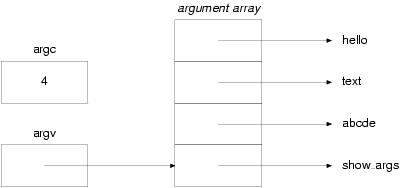
\includegraphics[type=pdf,read=.pdf,ext=.pdf,scale=0.9]
     {figure/10.1_argPrg}
     \caption*{Diagram showing the relationship between 'argc' and 'argv'                and the strings that elements of 'argv' point to}
     \caption{\label{fig:argPrg}Arguments to a program}
   \end{figure*}


  
  Each time that \texttt{argv} is incremented, it is stepped one item
   further along the array of arguments. Thus after the first iteration of
   the loop, \texttt{argv} will point to the pointer which in turn
   points to the \texttt{abcde} argument.  This is shown in
   Figure~\ref{fig:argPrgInc}.


   \begin{figure*}\centering
     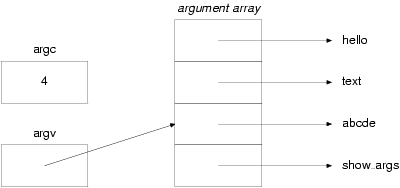
\includegraphics[type=pdf,read=.pdf,ext=.pdf,scale=0.9]
     {figure/10.2_argPrgInc}
     \caption*{Diagram showing the changes
       to the arrangement in Figure~\ref{fig:argPrg}
       after incrementing 'argv' so that it points to the next
       element in the array of pointers}
     \caption{\label{fig:argPrgInc}Arguments to a program after incrementing
       \texttt\{argv\}}
   \end{figure*}


  On the system where this program was tested, a program is run by typing
   its name and then the arguments, separated by spaces. This is what
   happened (the \texttt{\$} is a prompt):


  \begin{Verbatim}
$ show_args abcde text hello
show_args
abcde
text
hello
$
\end{Verbatim}

 
        \section{Interpreting program arguments}
        

  

  The loop used to examine the program arguments in the example above is
   a common C idiom which you will see in many other programs. An additional
   common idiom is to use `options' to control the behaviour of the
   program (these are also sometimes called switches or flags). Arguments which
   start with a `\texttt{-}' are taken to introduce one or more
   single-letter option indicators, which can be run together or provided
   separately:


  \begin{Verbatim}
progname -abxu file1 file2
progname -a -b -x -u file1 file2
\end{Verbatim}

  The idea is that each of the options selects a particular aspect from the
   program's repertoire of features. An extension to that idea is to allow
   options to take arguments; if the \texttt{-x} option is specified to
   take an argument, then this is how it might be used:


  \begin{Verbatim}
progname -x arg file1
\end{Verbatim}

  so that the \texttt{arg} argument is associated with the option. The
   \texttt{options} function below automates the processing of this style
   of use, with the additional (common but preferably considered obsolescent)
   support for the provision of option arguments immediately following the
   option letter, as in:


  \begin{Verbatim}
progname -xarg file1
\end{Verbatim}

  In either of the above cases, the options routine returns the character
   `\texttt{x}' and sets a global pointer, \texttt{OptArg}, to
   point to the value \texttt{arg}.


  To use this routine, a program must supply a list of valid option letters
   in the form of a string; when a letter in this string is followed by
   a `\texttt{:}' this indicates that the option letter is to be
   followed by an argument. When the program is run, it is then simply
   a question of repeatedly calling the \texttt{options} routine until no
   more option letters remain to be found.


  It seems to be a fact of life that functions which scan text strings
   looking for various combinations or patterns within them end up being hard
   to read; if it's any consolation they aren't all that easy to write either.
   The code that implements the options is definitely one of the breed,
   although by no means one of the worst:


  \VerbatimInput{example/example10-2.c}\begin{center}\textit{Example 10.2}\end{center}


 
        \section{A pattern matching program}
        

  

  This section presents a complete program which makes use of option letters
   as program arguments to control the way it performs its job.


  The program first processes any arguments that resemble options; the first
   argument which is not an option is remembered for use as a `search
   string'. Any remaining arguments are used to specify file names which are
   to be read as input to the program; if no file names are provided, the
   program reads from its standard input instead. If a match for the search
   string is found in a line of input text, that whole line is printed on the
   standard output.


  The \texttt{options} function is used to process all option letters
   supplied to the program. This program recognises five options:
   \texttt{-c}, \texttt{-i}, \texttt{-l}, \texttt{-n}, and
   \texttt{-v}. None of these options is required to be followed by an
   option argument. When the program is run with one or more of these options
   its behaviour is modified as follows:


  \begin{description}
   \item[\texttt{-c}] the program prints a count of the total number of matching lines it
    found in the input file(s). No lines of text are printed.

   \item[\texttt{-i}] when searching for a match, the case of letters in both the input lines
    and string is ignored.

   \item[\texttt{-l}] each line of text printed on the output is prefixed with the line number
    being examined in the current input file.

   \item[\texttt{-n}] each line of text printed on the output is prefixed with the name of the
    file that contained the line.

   \item[\texttt{-v}] the program prints only lines which do not match the string
    supplied.
  \end{description}

  When the program finishes, it returns an exit status to indicate one of
   the following situations:


  \begin{description}
   \item[\texttt{EXIT\_SUCCESS}] at least one match was found.
   \item[\texttt{EXIT\_FAILURE}] no match was found, or some error occurred.
  \end{description}

  The program makes extensive use of standard library functions to do all of
   the hard work. For example, all of the file handling is performed by calls
   to \texttt{stdio} functions. Notice too that the real heart of the
   program, the string matching, is simply handled by a call to the
   \texttt{strstr} library function.


  Here is the code for the whole program. Of course, to get this to work you
   would need to compile it together with the code for the options routine
   presented above.


  \VerbatimInput{example/example10-3.c}\begin{center}\textit{Example 10.3}\end{center}


 
        \section{A more ambitious example}
        

  

  Finally here is a set of programs designed to cooperate and manipulate
   a single data file in a coherent, robust fashion.


  The programs are intended to help keep track of a ladder of players who
   compete against each other at some game, squash or chess perhaps.


  Each player has a rank from one to n, where n is the number of players who
   play, one being the highest rank on the ladder. Players lower down the
   ladder may challenge players above them and, if the lower ranked player
   wins, he or she moves up taking the rank of the player who loses. The loser
   in such a situation, and any other players between challenger and loser, are
   then moved down one rank. If a challenger does not win, the rankings on the
   ladder remain unchanged.


  To provide some measure of equilibrium in the rankings, a player may
   challenge any higher ranked player, but only wins over players ranked three
   (or less) higher will allow the challenger to move up the rankings. This
   ensures that new players added to the bottom of the ladder are forced to
   play more than one game to reach the top of the ladder!


  There are three basic tasks which are required to record all the
   information needed to keep such a ladder going:


  \begin{itemize}
   \item Printing the ladder.
   \item Addition of new players.
   \item Recording of results.
  \end{itemize}

  The design to be used here provides a separate program to perform each of
   these tasks. Having made this decision it is clear that a number of
   operations needed by each program will be common to all three. For example,
   all three will need to read player records from the data file, at least two
   will need to write player records into the data file.


  This suggests that a good approach would be to design a `library' of
   functions which manipulate player records and the data file which may in
   turn be combined to make up the programs which maintain the ladder.


  Before this can be done it will be necessary to define the data structure
   which represents player records. The minimum information necessary to record
   for each player consists of player name and rank. However, to allow for more
   interesting statistics to be compiled about the ladder let us chose to also
   keep a record of games won, games lost and the time when the last game was
   played. Clearly this disparate set of information is best collected together
   in a structure.


  The player structure declaration together with the declarations of the
   player library functions are combined together in the \texttt{player.h}
   header file. The data file is maintained as lines of text, each line
   corresponding to a record; this requires input and output conversions to be
   performed but is a useful technique if the conversions don't cost too much
   in performance terms.


  \VerbatimInput{example/example10-4.c}\begin{center}\textit{Example 10.4}\end{center}


  Here is the code for the \texttt{player.c} file implementing the
   generic functions which manipulate player records and the data file. These
   functions can be combined with more specific routines to make up the three
   programs required to maintain the ladder.


  Notice that to manipulate the player records, each program is required to
   read the entire data file into a dynamically allocated array. Before this
   array is written back to the data file, it is assumed that the records it
   contains will have been sorted into rank order. If the records do not remain
   sorted, the \texttt{push\_down} function will produce some
   `interesting' results!


  \VerbatimInput{example/example10-5.c}\begin{center}\textit{Example 10.5}\end{center}


  This code, when tested, was compiled into an object file which was then
   linked (together with an object file containing the code for the
   \texttt{options} function) with one of the following three programs to
   for the ladder maintenance utilities.


  Here is the code for the simplest of those utilities,
   \texttt{showlddr} which is contained in the file
   \texttt{showlddr.c}.


  This program takes a single option, \texttt{-f}, which you will notice
   takes an option argument. The purpose of this argument is to allow you to
   print a ladder data file with a name other than the default file name,
   \texttt{ladder}.


  The player records in the data file should be stored pre-sorted but, just
   to be safe, \texttt{showlddr} sorts them before it prints them out.


  \VerbatimInput{example/example10-6.c}\begin{center}\textit{Example 10.6}\end{center}


  Of course the \texttt{showlddr} program works only if there is an
   existing data file containing player records in the correct format. The
   program newplyr creates such a file if one does not already exist and then
   adds a new player record, in the correct format to that file.


  Typically, new players are added at the bottom of the rankings but for the
   odd occasion where this really may not make sense, \texttt{newplyr} also
   allows a player to be inserted into the middle of the rankings.


  A player may only appear once on the ladder (unless a pseudonym is used!)
   and there can only be one player at any one rank. Thus the program checks
   for duplicate entries and if the new player is to be inserted into
   a middling rank, moves other players already on the ladder out of the
   way.


  As with the \texttt{showlddr} program, \texttt{newplyr} recognises
   a \texttt{-f} option as a request to add the new player to a file named
   by the option argument rather than the default file, ladder. In addition,
   newplyr requires two options, \texttt{-n} and \texttt{-r}, each with
   option arguments to specify both the new player's name and initial ranking
   respectively.


  \VerbatimInput{example/example10-7.c}\begin{center}\textit{Example 10.7}\end{center}


  The only remaining utility required is one for recording the results of
   games played. The \texttt{result} program performs this task.


  As with the previous two utilities, \texttt{result} will accept
   a \texttt{-f} option together with a file name to specify an alternative
   to the default player record file.


  Unlike the \texttt{newplyr} utility, \texttt{result} interactively
   prompts the user for the names of the winning and losing players. The
   program insists that the names supplied should be those of existing
   players.


  Given a valid pair of names, a check is then made to see if the loser is
   higher ranked than winner and whether or not the winner is ranked close
   enough for the victory to alter the rankings.


  If a change in the standings is in order, the victor takes the loser's
   rank and the loser (as well as any other player on an intervening rank) is
   demoted one rank.


  Here is the code for the \texttt{result} utility.


  \VerbatimInput{example/example10-8.c}\begin{center}\textit{Example 10.8}\end{center}

 
 
        \section{Afterword}
        

  

  The programs shown in this chapter should help to to get a feel for
   what middle-of-the-road C programs look like, using the language and
   libraries defined in the Standard.


  What do we mean by `middle-of-the-road'? Simply this: they have
   been designed, implemented, tested and documented in a way appropriate
   for small, self-contained programs that have no real need to show high
   levels of robustness and reliability. Many programs don't need to meet
   demanding criteria; to do more to them would be over-engineering.
   Clearly, it is entirely dependent on the eventual purpose for which the
   program is intended.


  There are situations which place very high demands on the software that
   is in use; programs to meet these requirements are very carefully
   engineered and have much higher amounts of effort put into reviewing,
   testing and the control of access to the source code than would be
   appropriate for simple illustrative example programs. C is also used in
   these application areas.  The source code of programs that meet such high
   requirements tends to look distinctively different; the language is the
   same, but the amount of error checking and correction is typically much
   higher. We have \textit{not} tried to illustrate that type of
   program.


  Whichever environment you work in, we hope that this book has helped
   you in your understanding of C. Good luck!


 \chapter*{Answers to Exercises}\addcontentsline{toc}{chapter}{Answers to Exercises}


        \section*{Chapter 1}\addcontentsline{toc}{section}{Chapter 1}
        

  

  \subsubsection*{Exercise 1.2}

   \begin{Verbatim}
#include <stdio.h>
#include <stdlib.h>

main(){
   int this_number, divisor, not_prime;
   int last_prime;

   this_number = 3;
   last_prime = 3;

   printf("1, 3 is a prime pair\n");

   while(this_number < 10000){
      divisor = this_number / 2;
      not_prime = 0;
      while(divisor > 1){
         if(this_number % divisor == 0){
            not_prime = 1;
            divisor = 0;
         }
         else
            divisor = divisor-1;
      }

      if(not_prime == 0){
         if(this_number == last_prime+2)
            printf("%d, %d is a prime pair\n",
               last_prime, this_number);
         last_prime = this_number;
      }
      this_number = this_number + 1;
   }
   exit(EXIT_SUCCESS);
}
\end{Verbatim}

  

  \subsubsection*{Exercise 1.3}

   \begin{Verbatim}
#include <stdio.h>
#include <stdlib.h>

main(){
   printf("Type in a string: ");
   printf("The value was: %d\n", getnum());
   exit(EXIT_SUCCESS);
}

getnum(){
   int c, value;;

   value = 0;
   c = getchar();
   while(c != '\n'){
      value = 10*value + c - '0';
      c = getchar();
   }
   return (value);
}
\end{Verbatim}

  

  \subsubsection*{Exercise 1.4}

   \begin{Verbatim}
#include <stdio.h>
#include <stdlib.h>

/* array size */
#define NUMBER  10

main(){
   int arr[NUMBER], count, lo, hi;

   count = 0;
   while(count < NUMBER){
      printf("Type in a string: ");
      arr[count] = getnum();
      count = count+1;
   }
   lo = 0;
   while(lo < NUMBER-1){
      hi = lo+1;
      while(hi < NUMBER){
         int tmp;
         if(arr[lo] > arr[hi]){
            tmp = arr[lo];
            arr[lo] = arr[hi];
            arr[hi] = tmp;
         }
         hi = hi + 1;
      }
      lo = lo + 1;
   }
   /* now print them */
   count = 0;
   while(count < NUMBER){
      printf("%d\n", arr[count]);
      count = count+1;
   }
   exit(EXIT_SUCCESS);
}

getnum(){
   int c, value;;

   value = 0;
   c = getchar();
   while(c != '\n'){
      value = 10*value + c - '0';
      c = getchar();
   }
   return (value);
}
\end{Verbatim}

  

  \subsubsection*{Exercise 1.5}

   \begin{Verbatim}
#include <stdio.h>
#include <stdlib.h>

/*
* To print an int in binary, hex, decimal,
* we build an array of characters and print it out
* in order.
* The values are found least significant digit first,
* and printed most significant digit first.
*/
#define NDIG    32      /* assume max no. of digits */

int getnum(void);

main(){
   int val, i, count;
   char chars[NDIG];

   i = getnum();

   /* print in binary */
   val = i;
   count = 0;
   do{
      chars[count] = val % 2;
      val = val / 2;
      count = count + 1;
   }while(val);
   count = count - 1; /* just incremented above */

   while(count >= 0){
      printf("%d", chars[count]);
      count = count - 1;
   }
   printf("\n");

   /* print in decimal */
   val = i;
   count = 0;
   do{
      chars[count] = val % 10;
      val = val / 10;
      count = count + 1;
   }while(val);
   count = count - 1; /* just incremented above */

   while(count >= 0){
      printf("%d", chars[count]);
      count = count - 1;
   }
   printf("\n");

   /* print in hex */
   val = i;
   count = 0;
   do{
      chars[count] = val % 16;
      val = val / 16;
      count = count + 1;
   }while(val);
   count = count - 1; /* just incremented above */

   while(count >= 0){
      if(chars[count] < 10)
         printf("%d", chars[count]);
      else{
         /* assume 'A' - 'F' consecutive */
         chars[count] = chars[count]-10+'A';
         printf("%c", chars[count]);
      }
      count = count - 1;
   }
   printf("\n");
   exit(EXIT_SUCCESS);
}

getnum(){
   int c, value;;

   value = 0;
   c = getchar();
   while(c != '\n'){
      value = 10*value + c - '0';
      c = getchar();
   }
   return (value);
}
\end{Verbatim}

  

 
        \section*{Chapter 2}\addcontentsline{toc}{section}{Chapter 2}
        

  

  \subsubsection*{Exercise 2.1}

   Trigraphs are used when the input device used, or the host system's
    native character set, do not support enough distinct characters for the
    full C language.


  

  \subsubsection*{Exercise 2.2}

   Trigraphs would not be used in a system that has enough distinct
    characters to allocate a separate one to each of the C language symbols.
    For maximum portability, one might see a trigraph representation of
    a C program being distributed, on the grounds that most systems which do
    not use ASCII will be able to read ASCII coded data and translate it into
    their native codeset.  A Standard C compiler could then compile such
    a program directly.


  

  \subsubsection*{Exercise 2.3}

   White space characters are not equivalent to each other inside strings
    and character constants. Newline is special to the preprocessor.


  

  \subsubsection*{Exercise 2.4}

   To continue a long line. Especially in systems that have an upper limit
    on physical line length.


  

  \subsubsection*{Exercise 2.5}

   They become joined.


  

  \subsubsection*{Exercise 2.6}

   Because the \texttt{*/} which apparently terminates the inner comment
    actually terminates the outer comment.


  

  \subsubsection*{Exercise 2.7}

   31 characters for internal variables, six for external variables. The six
    character names must not rely on distinction between upper and lower case,
    either.


  

  \subsubsection*{Exercise 2.8}

   A declaration introduces a name and a type for something. It does not
    necessarily reserve any storage.


  

  \subsubsection*{Exercise 2.9}

   A definition is a declaration that also reserves storage.


  

  \subsubsection*{Exercise 2.10}

   It is always the case that the largest range of values can be held in
    a long double, although it may not actually be any different from one of
    the smaller floating point types.


  

  \subsubsection*{Exercise 2.11}

   The same answer holds true for the type with the greatest precision: long
    double. C does not permit the language implementor to use the same number
    of bits for, say, double and long double, then to allocate more bits for
    precision in one type and more for range in the other.


  

  \subsubsection*{Exercise 2.12}

   There can never be problems assigning a shorter floating point type to
    a longer one.


  

  \subsubsection*{Exercise 2.13}

   Assigning a longer floating type to a shorter one can result in overflow
    and undefined behaviour.


  

  \subsubsection*{Exercise 2.14}

   Undefined behaviour is completely unpredictable. Anything may happen.
    Often, nothing seems to happen except that erroneous arithmetic values are
    produced.


  

  \subsubsection*{Exercise 2.15}

   \begin{enumerate}
    \item \texttt{Signed int} (by the integral promotions).

    \item This cannot be predicted without knowing about the implementation.
     If an \kint{} can hold all of the values of an \texttt{unsigned
     char} the result will be \kint, again by the integral
     promotions. Otherwise, it will have to be \texttt{unsigned int}.

    \item \texttt{Unsigned int}.
    \item \klong.
    \item \texttt{Unsigned long}.
    \item \klong.
    \item \float.
    \item \float.
    \item \texttt{Long double}.
   \end{enumerate}

  

  \subsubsection*{Exercise 2.16}

   \begin{enumerate}
    \item \texttt{i1 \% i2}
    \item \texttt{i1 \% (int)f1}

    \item If either operand is negative, the sign is implementation defined,
     otherwise it is positive. This means that, even if both operands are
     negative, you can't predict the sign.

    \item Two--unary negate, binary subtract.

    \item \texttt{i1 \&= 0xf;}
    \item \texttt{i1 |= 0xf;}
    \item \texttt{i1 \&= \~{}0xf;}
    \item \texttt{i1 = ((i2 >{}> 4) \& 0xf) | ((i2 \& 0xf) <{}< 4);}

    \item The result is unpredictable. You must never use the same variable more
     than once in an expression if the expression changes its value.
   \end{enumerate}

  

  \subsubsection*{Exercise 2.17}

   \begin{enumerate}

    \item 
     \begin{Verbatim}
(c = (( u * f) + 2.6L);
(int = ((float) + long double);
(int = (long double));
(int);
\end{Verbatim}

     Note: the integral promotion of \kchar{} to \kint{}
      might be to \texttt{unsigned int}, depending on the
      implementation.


    

    \item 
     \begin{Verbatim}
(u += (((--f) / u) % 3));
(unsigned += ((float / unsigned) % int));
(unsigned += (float % int));
(unsigned += float);
(unsigned);
\end{Verbatim}

    

    \item 
     \begin{Verbatim}
       (i   <{}<= (u * (- (++f))));
       (int <{}<= (unsigned * (- float)));
       (int <{}<= (unsigned * float));
       (int <{}<= float);
       (int);
     \end{Verbatim}

     The rules for the shift operators state the right-hand operand is
      always converted to \kint. However, this does not affect the
      result, whose type is always determined by the type of the left-hand
      operand. This is doubly so for the current example, since an assignment
      operator is being used.


    

    \item 
     \begin{Verbatim}
(u = (((i + 3) + 4) + 3.1));
\end{Verbatim}

     The rules state that the subexpressions involving \texttt{+} can be
      arbitrarily regrouped, as long as no type changes would be introduced.
      The types are:


     \begin{Verbatim}
(unsigned = (((int + int) + int) + double))
\end{Verbatim}

     so the leftmost two additions can be regrouped. Working from the
      left:


     \begin{Verbatim}
(unsigned = ((int + int) + double));
(unsigned = (int + double));
(unsigned = double);
(unsigned);
\end{Verbatim}

    

    \item 
     \begin{Verbatim}
(u = (((3.1 + i) + 3 ) + 4));
\end{Verbatim}

     See the comments above on regrouping.


     \begin{Verbatim}
(unsigned = (((double + int) + int) + int));
\end{Verbatim}

     The two rightmost additions can be regrouped.


     \begin{Verbatim}
(unsigned = ((double + int) + int));
(unsigned = (double + int));
(unsigned = double);
(unsigned);
\end{Verbatim}

    

    \item 
     \begin{Verbatim}
(c    = ((i   <{}< (- (--f))) & 0xf));
(char = ((int <{}< (- (--float))) & int ));
(char = ((int <{}< (- float)) & int ));
(char = ((int <{}< float) & int));
(char = (int & int));
(char);
\end{Verbatim}

    

   \end{enumerate}

  

 
        \section*{Chapter 3}\addcontentsline{toc}{section}{Chapter 3}
        

  

  \subsubsection*{Exercise 3.1}

   They all give an \kint{} result with a value of \texttt{1}
    for true and \texttt{0} for false.


  

  \subsubsection*{Exercise 3.2}

   They all give an \kint{} result with a value of \texttt{1}
    for true and \texttt{0} for false.


  

  \subsubsection*{Exercise 3.3}

   They guarantee an order of evaluation: left to right, and stop as soon as
    the overall result can be determined.


  

  \subsubsection*{Exercise 3.4}

   \kbreak{} can be used to turn a \switch{} statement
    into a set of exclusive choices of action.


  

  \subsubsection*{Exercise 3.5}

  \continue{} has no special meaning in a \switch{} statement,
  but only to an outer \kdo, \while{} or \for{} statement.


  

  \subsubsection*{Exercise 3.6}

   Inside a \while{} statement, the use of continue may cause the
    update of the loop control variable to be missed. It is, of course, the
    responsibility of the programmer to get this right.


  

  \subsubsection*{Exercise 3.7}

  Because the scope of a label doesn't extend outside the function that it
  lives in, you can't use goto to jump from one function to another. Using
  the \texttt{longjmp} library routine, described in Chapter~\ref{chap:libs},
  a form of function-to-function jump is supported, but not
  a completely general one.


  

 
        \section*{Chapter 4}\addcontentsline{toc}{section}{Chapter 4}
        

  

  \subsubsection*{Exercise 4.1}

   \begin{Verbatim}
#include <stdio.h>
#include <stdlib.h>

main(){
  int i, abs_val(int);;

  for(i = -10; i <= 10; i++)
    printf("abs of %d is %d\n", i, abs_val(i));
  exit(EXIT_SUCCESS);
}

int
abs_val(int x){

  if(x < 0)
    return(-x);
  return(x);
}
\end{Verbatim}

  

  \subsubsection*{Exercise 4.2}

   There are two files that form the answer to this exercise. This is the
    first.


   \begin{Verbatim}
#include <stdio.h>
#include <stdlib.h>

int curr_line(void), curr_col(void);
void output(char);

main(){
  printf("line %d\n", curr_line());
  printf("column %d\n", curr_col());

  output('a');
  printf("column %d\n", curr_col());

  output('\n');
  printf("line %d\n", curr_line());
  printf("column %d\n", curr_col());
  exit(EXIT_SUCCESS);
}
\end{Verbatim}

   The second file contains the functions and static variables.


   \begin{Verbatim}
#include <stdio.h>

int curr_line(void), curr_col(void);
void output(char);

static int lineno=1, colno=1;

int
curr_line(void){
  return(lineno);
}

int
curr_col(void){
  return(colno);
}

void
output(char a){
  putchar(a);
  colno++;
  if(a == '\n'){
    colno = 1;
    lineno++;
  }
}
\end{Verbatim}

  

  \subsubsection*{Exercise 4.3}

   The recursive function:


   \begin{Verbatim}
#include <stdio.h>
#include <stdlib.h>

void recur(void);

main(){
  recur();
  exit(EXIT_SUCCESS);
}

void
recur(void){
  static ntimes;

  ntimes++;
    if(ntimes < 100)
      recur();
  printf("%d\n", ntimes);
  ntimes--;
}
\end{Verbatim}

  

  \subsubsection*{Exercise 4.4}

   And finally, the largest of all of the answers.


   \begin{Verbatim}
#include <stdio.h>
#include <stdlib.h>

#define PI 3.141592
#define INCREMENT (PI/20)
#define DELTA .0001

double sine(double), cosine(double);
static unsigned int fact(unsigned int n);
static double pow(double x, unsigned int n);

main(){
  double arg = 0;

  for(arg = 0; arg <= PI; arg += INCREMENT){
    printf("value %f\tsine %f\tcosine %f\n", arg, sine(arg), cosine(arg));
  }
  exit(EXIT_SUCCESS);
}

static unsigned int
fact(unsigned int n){
  unsigned int answer;

  answer = 1;
  while(n > 1)
    answer *= n--;

  return(answer);
}

static double
pow(double x, unsigned int n){
  double answer;

  answer = 1;
  while(n){
    answer *= x;
    n--;
  }
  return(answer);
}

double
sine(double x){
  double difference, thisval, lastval;
  unsigned int term;
  int sign;

  sign = -1;
  term = 3;

  thisval = x;
  do{
    lastval = thisval;
    thisval = lastval + pow(x, term)/fact(term) * sign;
    term += 2;
    sign = -sign;
    difference = thisval - lastval;
    if(difference < 0)
      difference = -difference;
    }while(difference > DELTA && term < 16);

  return(thisval);
}

double
cosine(double x){
double difference, thisval, lastval;
  unsigned int term;
  int sign;

  sign = -1;
  term = 2;

  thisval = 1;
  do{
    lastval = thisval;
    thisval = lastval + pow(x, term)/fact(term)  * sign;
    term += 2;
    sign = -sign;
    difference = thisval - lastval;
    if(difference < 0)
      difference = -difference;
  }while(difference > DELTA && term < 16);

  return(thisval);
}
\end{Verbatim}

  

 
        \section*{Chapter 5}\addcontentsline{toc}{section}{Chapter 5}
        

  

  \subsubsection*{Exercise 5.1}

   \texttt{0-9}.


  

  \subsubsection*{Exercise 5.2}

   Nothing. It is guaranteed to be a valid address and can be used to check
    a pointer against the end of the array.


  

  \subsubsection*{Exercise 5.3}

   Only when they point into the same array, or to the same object.


  

  \subsubsection*{Exercise 5.4}

   It can safely be used to hold the value of a pointer to any sort of
    object.


  

  \subsubsection*{Exercise 5.5}

   \begin{enumerate}

    \item 
     \begin{Verbatim}
int
st_eq(const char *s1, const char * s2){

  while(*s1 && *s2 && (*s1 == *s2)){
    s1++; s2++;
  }

  return(*s1-*s2);
}
\end{Verbatim}

    

    \item 
     \begin{Verbatim}
const char *
find_c(char c, const char *cp){

  while(*cp && *cp != c)
     cp++;
  if(*cp)
    return(cp);

  return(0);
}
\end{Verbatim}

    

    \item 
     \begin{Verbatim}
const char *
sub_st(const char *target, const char *sample){

  /*
   * Try for a substring starting with
   * each character in sample.
  */
  while(*sample){
    const char *targ_p, *sample_p;

    targ_p = target;
    sample_p = sample;
    /* string compare */
    while(*targ_p && *sample_p && (*targ_p == *sample_p)){
        targ_p++; sample_p++;
    }
    /*
    * If at end of target, have substring!
    */
    if(*targ_p == 0)
      return(sample);
    /* otherwise try next place */
      sample++;
    }
  return(0);      /* no match */
}
\end{Verbatim}

    

   \end{enumerate}

  

  \subsubsection*{Exercise 5.6}

   No answer can be given.


  

 
        \section*{Chapter 6}\addcontentsline{toc}{section}{Chapter 6}
        

  

  \subsubsection*{Exercise 6.1}

   \begin{Verbatim}
struct {
  int a,b;
};
\end{Verbatim}

  

  \subsubsection*{Exercise 6.2}

   Without a tag or any variables defined, the structure declaration is of
    little use. It cannot be referred to later.


  

  \subsubsection*{Exercise 6.3}

   \begin{Verbatim}
struct int_struc{
  int a,b;
}x,y;
\end{Verbatim}

  

  \subsubsection*{Exercise 6.4}

   \begin{Verbatim}
struct int_struc z;
\end{Verbatim}

  

  \subsubsection*{Exercise 6.5}

   \begin{Verbatim}
p = &z;
p->a = 0;
\end{Verbatim}

  

  \subsubsection*{Exercise 6.6}

   Explicitly, for example


   \begin{Verbatim}
struct x;
\end{Verbatim}

   or implicitly,


   \begin{Verbatim}
struct x *p;
\end{Verbatim}

   when no outer declaration exists.


  

  \subsubsection*{Exercise 6.7}

   It is not treated as a pointer, but as a short-hand way of initializing
    the individual array elements.


  

  \subsubsection*{Exercise 6.8}

   Nothing unusual at all, the string is treated as a literal constant of
    type \texttt{const char *}.


  

  \subsubsection*{Exercise 6.9}

   Yes. It is easier!


  

 
        \section*{Chapter 7}\addcontentsline{toc}{section}{Chapter 7}
        

  

  \subsubsection*{Exercise 7.1}

   \begin{Verbatim}
#define MAXLEN 100
\end{Verbatim}

  

  \subsubsection*{Exercise 7.2}

   In expressions, there may be precedence problems. A safer definition
    would be \texttt{\#define VALUE (100+MAXLEN)}.


  

  \subsubsection*{Exercise 7.3}

   \begin{Verbatim}
#define REM(a,b) ((a)%(b))
\end{Verbatim}

  

  \subsubsection*{Exercise 7.4}

   \begin{Verbatim}
#define REM(a,b) ((long)(a)%(long)(b))
\end{Verbatim}

  

  \subsubsection*{Exercise 7.5}

   It generally signifies a library header file.


  

  \subsubsection*{Exercise 7.6}

   It generally signifies a private header file.


  

  \subsubsection*{Exercise 7.7}

   By using the conditional compilation directives. Examples are shown in
    the text.


  

  \subsubsection*{Exercise 7.8}

   It uses long int in place of int and unsigned long int, in place of
    unsigned int using the arithmetic environment provided by the translator,
    not the target. It must provide at least the ranges described in
    \texttt{<limits.h>}.


  

 

%%% Local Variables:
%%% mode: latex
%%% TeX-master: "thecbook"
%%% End:



\bibliographystyle{apalike}
\bibliography{bib}{}
\end{document}
